%%%%%%%%%%%%%%%%%%%%%%%%%%%%%%%%%%%%%%%%%%%%%%%%%%%%%%%%%%%%%%%%%%%%%%
% James Bueghly's Northwestern Ph.D. Thesis
% Department of Physics and Astronomy
% CMS Run II Higgs to Z+gamma Analysis
%%%%%%%%%%%%%%%%%%%%%%%%%%%%%%%%%%%%%%%%%%%%%%%%%%%%%%%%%%%%%%%%%%%%%%

%%%%%%%%%%%%%%%%%%%%%%%%%%%%%%%%%%%%%%%%%%%%%%%%%%%%%%%%%%%%%%%%%%%%%%
% template from Northwestern Department of Mathematics
% nuthesis-template.tex - Miguel A, Lerma - 4/23/2018
%                         mlerma@math.northwestern.edu
%%%%%%%%%%%%%%%%%%%%%%%%%%%%%%%%%%%%%%%%%%%%%%%%%%%%%%%%%%%%%%%%%%%%%%

% The nuthesis class is based on % amsbook.cls.
\documentclass[12pt]{template/nuthesis}	
\usepackage{xcolor}
\usepackage{graphicx}
\usepackage{subcaption}
\usepackage{multirow}
\usepackage{cmsstyle/heppennames2}
\usepackage{cmsstyle/hepparticles}
\usepackage{cmsstyle/ptdr-definitions}
\newcommand\numberthis{\addtocounter{equation}{1}\tag{\theequation}}
\newcommand{\tabincell}[2]{\begin{tabular}{@{}#1@{}}#2\end{tabular}}
\newcommand{\LumiT}{138}
\newcommand{\Lumia}{36.3}
\newcommand{\Lumib}{41.5} 
\newcommand{\Lumic}{59.8}
\newcommand{\mH}{125.38}
\newcommand{\signalstrength}{\ensuremath{2.4\pm0.9}}
\newcommand{\signalstrengthExpanded}{\ensuremath{2.4^{+0.8}_{-0.9}}\,\stat\,^{+0.3}_{-0.2}\,\syst}
\newcommand{\signalstrengthdijetthree}{\ensuremath{12.3^{+3.7}_{-3.5}}}
\newcommand{\br}{$0.21\pm0.08$}
\newcommand{\brExpanded}{\ensuremath{0.21^{+0.07}_{-0.08}\,\stat\,^{+0.03}_{-0.02}\,\syst}}
\newcommand{\explimit}{1.8}
\newcommand{\obslimit}{4.1}
\newcommand{\expsig}{1.2}
\newcommand{\obssig}{2.7}
\newcommand{\compatibility}{1.6}
\newcommand{\brRatio}{\ensuremath{1.5^{+0.7}_{-0.6}}}
\newcommand{\brRatioCompat}{1.5}
\newcommand{\channelcompatp}{0.02}
\newcommand{\channelcompatsigma}{2.3}

% shortcuts and values
\newcommand{\hzg}{$\PH \to \PZ \gamma$}
\newcommand{\hmumu}{$H \rightarrow \mu^{+}\mu^{-}$}
\newcommand{\hgg}{$H \rightarrow \gamma\gamma$}
\newcommand{\hzz}{$H \rightarrow ZZ$}
\newcommand{\pT}{$p_{T}$}

\author{James Bueghly}

\title{Search for Higgs Boson Decays to a Z Boson and a Photon}

%\degree{DOCTOR OF PHILOSOPHY}  % Default: DOCTOR OF PHILOSOPHY

\field{Physics and Astronomy}            % Default: Mathematics

\graduationmonth{March}         % The default is June or December
                                % depending on current date.

\graduationyear{2022}          % Default: current year.


				% Use \includeonly to select the 
%\includeonly{chap1,chap2,...}	% chapters to include if you are 
				% using the \include command below.
				% This way you can latex only a the 
				% part you are working on, which 
				% is faster than latexing the entire 
				% thesis. 


\begin{document}
%	
%	THE BODY OF YOUR THESIS STARTS HERE
%

%%%%%%%%%%%%%%%%%%%%%%
% Some initial stuff %
%%%%%%%%%%%%%%%%%%%%%%

\frontmatter		% Preliminary pages start here.

\maketitle		% Produces the title page.

\copyrightpage		% Creates the copyright page.


% Abstract.
\abstract

Since its discovery in 2012 at the Large Hadron Collider (LHC), efforts have been made to measure and characterize the properties of the Higgs boson. 
Among these efforts have been searches for rare decays of the Higgs predicted by the standard model (SM) of particle physics. 
One such decay is the process \hzg, which has an expected branching fraction of $\mathcal{B}(\PH\to\PZ\gamma) = (1.57 \pm 0.09) \times 10^{-3}$ in the SM, 
assuming a Higgs boson mass of $m_\PH = \mH\GeV$.
This decay mode has not yet been experimentally observed, and its observation and measurement remains an important goal of Higgs physics research at the LHC.
In addition, a measurement of this decay mode at a rate deviating from the SM prediction would provide indirect evidence of new physics beyond the SM (BSM). 

This thesis presents a search for \hzg, where $\mathrm{Z}\to\ell^+\ell^-$ with $\ell=\mathrm{e}$ or $\mu$. The search is performed using a sample of proton-proton ($\mathrm{pp}$) collision data at a center-of-mass energy of $13~\mathrm{TeV}$, recorded by the Compact Muon Solenoid (CMS) experiment at the LHC, corresponding to an integrated luminosity of $138~\mathrm{fb}^{-1}$. 
Events are assigned to mutually exclusive categories, which exploit differences in both event topology and kinematics of distinct Higgs production mechanisms to enhance signal sensitivity. 
To detect a potential signal, fits are performed to the distributions of ${\ell^+\ell^-\gamma}$ invariant mass in each of these categories simultaneously.
The signal strength $\mu$, defined as the product of the cross section and the branching fraction [$\sigma(\mathrm{pp}\to\mathrm{H})\mathcal{B}(\mathrm{H}\to\mathrm{Z}\gamma)$] relative to the SM expectation, is found to be $\mu= 2.4\,\pm0.9$ for $m_\PH = \mH\GeV$. This measurement corresponds to $\sigma(\mathrm{pp}\to\mathrm{H})\mathcal{B}(\mathrm{H}\to\mathrm{Z}\gamma)=0.21\pm0.08~\mathrm{pb}$. The statistical significance of the observed excess of events is $2.7$ standard deviations. The observed (expected) upper limit at $95$\% confidence level (CL) on $\mu$ is $4.1$\,($1.8$). 
The ratio of branching fractions $\mathcal{B}(\mathrm{H}\to\mathrm{Z}\gamma)/\mathcal{B}(\mathrm{H}\to\gamma\gamma)$ is measured to be $1.5^{+0.7}_{-0.6}$, which agrees with the SM prediction at the 
$1.5$ standard deviation level. 


\acknowledgements	% Acknowledgements (optional).

I would like to thank my adviser, Mayda Velasco, for giving me the opportunity to pursue a goal I dreamed up many years ago and for supporting me along the way. I'd also like to thank the many colleagues at Northwestern University, National Central University in Taiwan, CERN, and Fermilab who helped me grow both as a scientist and a person over the last six and a half years. 

Special thanks are due to those who significantly impacted the work contained in this thesis: My coanalyzer Ming-Yan Lee, whose discipline and tireless work ethic kept us all going through the many challenges we faced; postdoc Andrew Gilbert, whose expertise and guidance were critical; and the CMS leaders who guided and reviewed our work, including the Higgs conveners, Analysis Review Committee, and our colleague and language editor Jeff Richman. Without all of you, this thesis would not exist.

To my Northwestern colleagues: I will always be grateful for your friendship over these years. Those moments we shared away from the work kept me happy, sane, focused, and balanced. It is impossible to name all of them, but the squash games with Nate Odell, the lunches with Nate, Brian Pollack, Thoth Gunter, and Joseph Cordero Mercado, and the adventures at COFI in San Juan were just as meaningful to me as the work itself. 

Last, but not least, I want to thank my parents, sisters, and my partner Anna. You all have shown me so much love, encouragement, and patience throughout this process. For that, I feel extremely fortunate. This is for all of you. 



%\preface		% Preface (optional).
%
%This is the preface.


%% A few more optional pages (uncomment if needed)
%
%\listofabbreviations 
%
%This is the list of abbreviations (optional).
%
%\glossary
%
%This is the glossary (optional).
%
%\nomenclature
%
%This is the nomenclature (optional).
%
%% Note that the dedication text must be passed as an argument
%% of the \dedication command
%\dedication{This is the dedication (optional).}
%

\clearpage\phantomsection % needed for the hyperlinks to work correctly
\tableofcontents	% Table of Contents will be automatically
			% generated and placed here.

\clearpage\phantomsection % needed for the hyperlinks to work correctly
\listoftables		% List of Tables and List of Figures will be placed

\clearpage\phantomsection % needed for the hyperlinks to work correctly
\listoffigures		% here, if applicable (optional).



\mainmatter             % Actual text starts here.

%%%%%%%%%%%%%%%%%%%%%%%%%%%
% Actual text starts here %
%%%%%%%%%%%%%%%%%%%%%%%%%%%

% If there is an introduction it must be the first chapter

%\chapter{Introduction or Title of First Chapter}	% The first chapter.
%				% \chapter command is of the form
%				% \chapter[..]{..} or \chapter{..} where
%	... text ...		% {chapter heading} and [entry in table of
%				% contents].
%\section{First section of chapter 1}
%				% IMPORTANT: If your chapter heading consists
%				% of more than one lines, it will be auto-
%	... text ...		% matically broken into separate lines.
%				% However, if you don't like the way LaTeX
%				% breaks the chapter heading into lines, use
%\section{Another section}	% `\newheadline' command to break lines.
%				% Never use \\ in sectional (e.g., chapter,
%	... text ...		% section, subsection) headings.
%
%\chapter{Title of Second Chapter}	% Chapter 2.
%
%	... text ...
%
%\section{First section of chapter 2}
%
%	... text...
%
%\subsection{A subsection}
%
%	... more text ...
%
%\subsubsection{A subsubsection}
%
%	... more text ...


% Alternatively, you may write the chapters in separate
% files, say chap1.tex, chap2.tex, etc., and include them 
% with commands:

%\include{chap1}

%\include{chap2}

% The command \includeonly above allows to include a selected 
% set of chapters only.


\chapter{Introduction}

The standard model (SM) of particle physics is one of the most successful physics theories in history. It describes all of the fundamental particles we currently know in our universe, including the ways in which those particles interact with one another. Since its development in the second half of the twentieth century, the SM has been extensively tested through many measurements by numerous experiments. The Large Hadron Collider (LHC) was built with the goal of further testing the SM, while also searching for possible beyond the SM (BSM) physics at groundbreaking energy scales. One of the main goals of the LHC was to search for and observe the Higgs boson, a critical piece of the SM associated with the origin of particle mass.

Since the discovery of the Higgs boson~\cite{Aad_2012,Chatrchyan_2012,CMS:2013btf} at the LHC, an extensive program of measurements~\cite{PhysRevD.98.030001} has been undertaken to determine its properties and couplings to different types of particles and to assess whether these properties are consistent with those predicted by the SM. With the successful running of the LHC, large data samples of proton-proton ($\Pp\Pp$) collisions at $\sqrt s = 13\TeV$ have been accumulated, increasing the sensitivity to rare decays of the Higgs boson. 
Such decays also provide probes for possible contributions arising from BSM physics and include the process 
\hzg~\cite{Abba96, Chen12, Htollg-FB-Sun, Passarino, Campbell_2013hz, Degrassi:2019yix, Low:2011gn}.

Figure \ref{fig:fey} shows Feynman diagrams for the key SM contributions to the \hzg{} decay process. 
Experimentally, the final state resulting from $\PZ \to \ell^+ \ell^-$ ($\ell = \Pe$ or $\mu$) is the most accessible, since the leptons are highly distinctive, well-measured, and provide a means to trigger the recording of the events. 
\begin{figure*}[!b]
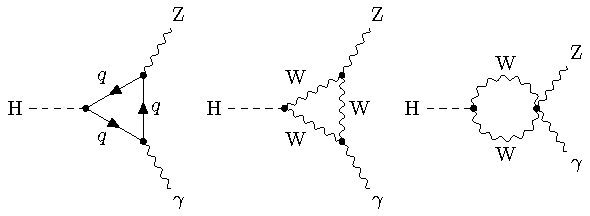
\includegraphics[width=0.9\textwidth]{fig/intro/Figure_001.pdf}
	\caption{Feynman diagrams for \hzg{} decay.} \label{fig:fey}
\end{figure*}
In the SM, the expected branching fraction for \hzg{} is $\mathcal{B}(\PH\to\PZ\gamma) = (1.57 \pm 0.09) \times 10^{-3}$, assuming a Higgs boson mass of $m_\PH = \mH\GeV$. This branching fraction is comparable to $\mathcal{B}(\PH\to\gamma\gamma)  = (2.27 \pm 0.04) \times 10^{-3}$~\cite{LHC-YR4,CMS:2021kom}. The value $m_\PH=\mH \pm 0.14\GeV$ is taken from the most recent Compact Muon Solenoid (CMS) Higgs boson mass measurement~\cite{CMS:2020xrn}, which uses the combination of $\PH\to\gamma\gamma$ and $\PH\to\PZ\PZ^*\to 4\ell$ results from the $2011$--$2012$ and $2016$ data samples.
The ratio $\mathcal{B}(\PH\to\PZ\gamma)/\mathcal{B}(\PH\rightarrow\gamma\gamma) = 0.69 \pm 0.04$ is 
potentially sensitive to BSM physics, such as supersymmetry (SUSY) and extended Higgs 
sectors~\cite{Djouadi:1996yq,Zg_theory_decaywidth,Zg_theory_extension,Chen:2013vi}.
The effects from these models can shift the \hzg{} and $\PH\to\PGg\PGg$ branching fractions 
by different amounts, making the ratio the most sensitive observable. 
The impact on the ratio varies by model, but can be up to 20\% for two Higgs doublet or minimal SUSY models.

The ATLAS (A Toroidal LHC ApparatuS) and CMS Collaborations have performed
searches for the decay $\PH\to\PZ\gamma\to\ell^+\ell^-\gamma$~\cite{atl-HZG,cms-HZG,Sirunyan:2018tbk,Aad:2020plj} at $\sqrt{s}=7$,
$8$, and $13\TeV$ in the $\Pe^+\Pe^-\gamma$ and $\mu^+\mu^-\gamma$ final states. 
The most stringent bound has been set by the ATLAS Collaboration using $\sqrt s = 13\TeV$ data corresponding to an integrated luminosity of $139\fbinv$. The observed (expected) upper limit at 95\% confidence level (\CL) on $\sigma(\Pp\Pp\to\PH)\mathcal{B}(\PH\to\PZ\gamma)$ relative to the SM is $3.6$ ($2.6$), assuming $m_\PH=125.09\GeV$.
The ATLAS experiment has reported evidence at the 3.2 standard deviation level for the decay $\PH\to\ell^+\ell^-\gamma$ with $m_{\ell^+\ell^-} < 30\GeV$ using both of the dilepton channels~\cite{atlas_llgrun2}.
The CMS Collaboration has also searched for the
$\PH\to\ell^+\ell^-\gamma$ process with $m_{\ell^+\ell^-} < 50\GeV$\, in the dimuon channel at $\sqrt{s}=8$~\cite{2016341} and
$13$~\cite{Sirunyan:2018tbk}$\TeV$.  

This thesis describes a search for the decay $\PH\to \PZ\gamma$, where $\PZ\to\ell^+\ell^-$ and $m_{\ell^+\ell^-} > 50$ \GeV. 
This phase space is chosen in order to target on-shell Z bosons, since the region $m_{\ell^+\ell^-} < 50$ \GeV contains a contribution from an additional process, $\PH \to \gamma^* \gamma \to \ell^+ \ell^- \gamma$~\cite{Htollg-FB-Sun}.
The data sample corresponds to an integrated luminosity of \LumiT\fbinv of $\Pp\Pp$ collisions at $\sqrt s = 13 \TeV$ accumulated between 2016 and 2018 by the CMS detector at the LHC. 
%The region at small dilepton invariant mass, $m_{\ell^+\ell^-} < 50$ \GeV, is excluded from the analysis. It contains a contribution from an additional process, $\PH \to \gamma^* \gamma \to \ell^+ \ell^- \gamma$~\cite{Htollg-FB-Sun}.
%The sensitivity of the analysis is enhanced by searching for Higgs boson production in a variety of mechanisms, including gluon-gluon fusion ($\Pg\Pg\PH$); vector boson fusion (VBF)
%; and the associated production of a Higgs boson with either weak vector bosons (V$\PH$, where V = $\PZ$ or $\PW$) or top quark pairs ($\ttbar\PH$). The dominant backgrounds arise from Drell--Yan production in association with an initial-state photon~($\PZ/\gamma^{*}$+$\gamma$) and Drell--Yan production in association with jets, where a jet or additional lepton is misidentified as a photon ($\PZ/\gamma^{*}$+jets). 
%After using a variety of discriminating variables to suppress background in the different production mechanisms, the signal is identified as a narrow resonant peak around $m_\PH$ in the distribution of the $\ell^+\ell^-\gamma$ invariant mass ($m_{\ell^{+}\ell^{-}\gamma}$).
%
%The data sample is divided into eight mutually exclusive categories according to (i) the presence of an additional lepton produced by $\PZ(\to\ell^+\ell^-)$ or $\PW(\to\ell\nu)$ decay, indicating the possible associated production of a Higgs boson with $\PW$ or $\PZ$ bosons, or $\ttbar\PH$ production with a leptonic top quark decay; (ii) the value of a multivariate analysis (MVA) discriminant characterizing the kinematic properties of a dijet system together with the $\ell^+\ell^-\gamma$ candidate, indicating possible VBF production; and (iii) the value of an MVA discriminant characterizing the kinematic properties of the $\ell^+\ell^-\gamma$ system. A simultaneous maximum likelihood fit is performed to the $m_{\ell^+\ell^-\gamma}$ distribution in each category. 
This thesis is organized as follows. The relevant theoretical physics background is provided in Chapter~\ref{sec:theory}, and the CMS detector and event reconstruction are described in Chapter~\ref{sec:experiment}. Chapter~\ref{sec:analysis_overview} provides an overview of the \hzg{} search strategy, and the data and simulated event samples are described in Chapter~\ref{sec:data}. Chapter~\ref{sec:selection} outlines the object and event selection, and Chapter~\ref{sec:categorization} discusses event categorization. The statistical procedure, including signal and background modeling, is presented in Chapter~\ref{sec:statistics}, with systematic uncertainties discussed in Chapter~\ref{sec:uncertainties}. The final results of the search are discussed in Chapter~\ref{sec:results}, followed by a conclusion in Chapter~\ref{sec:conclusion}.


\chapter{Theory}\label{sec:theory}

\section{The Standard Model}

The SM is currently our best theoretical framework for understanding the nature of fundamental particles. 
It is rooted in the idea that particles exist as excitations of quantum fields. These fields are constructed so as to obey 
fundamental symmetries of nature, and quantum field theory describes both the particles of our universe and their interactions. The SM is not only 
elegant and extensive, but provides a wide variety of measurable observables for the experimentalist to probe. So far, many 
measurements have been made of the known elementary particles and their interactions, and the predictions of the SM have held up in each case. In 
this respect, it is a wildly successful theory. In other respects, it is obviously incomplete. It does not account for the gravitational force, dark matter, or dark energy, among other phenomena. 
Thus, there is value in testing the SM even more carefully with experiments 
like those at the LHC, in hopes of refining our understanding and potentially discovering new physics. 

\section{The Elementary Particles} 

\begin{figure}[htb]
	\begin{center}
	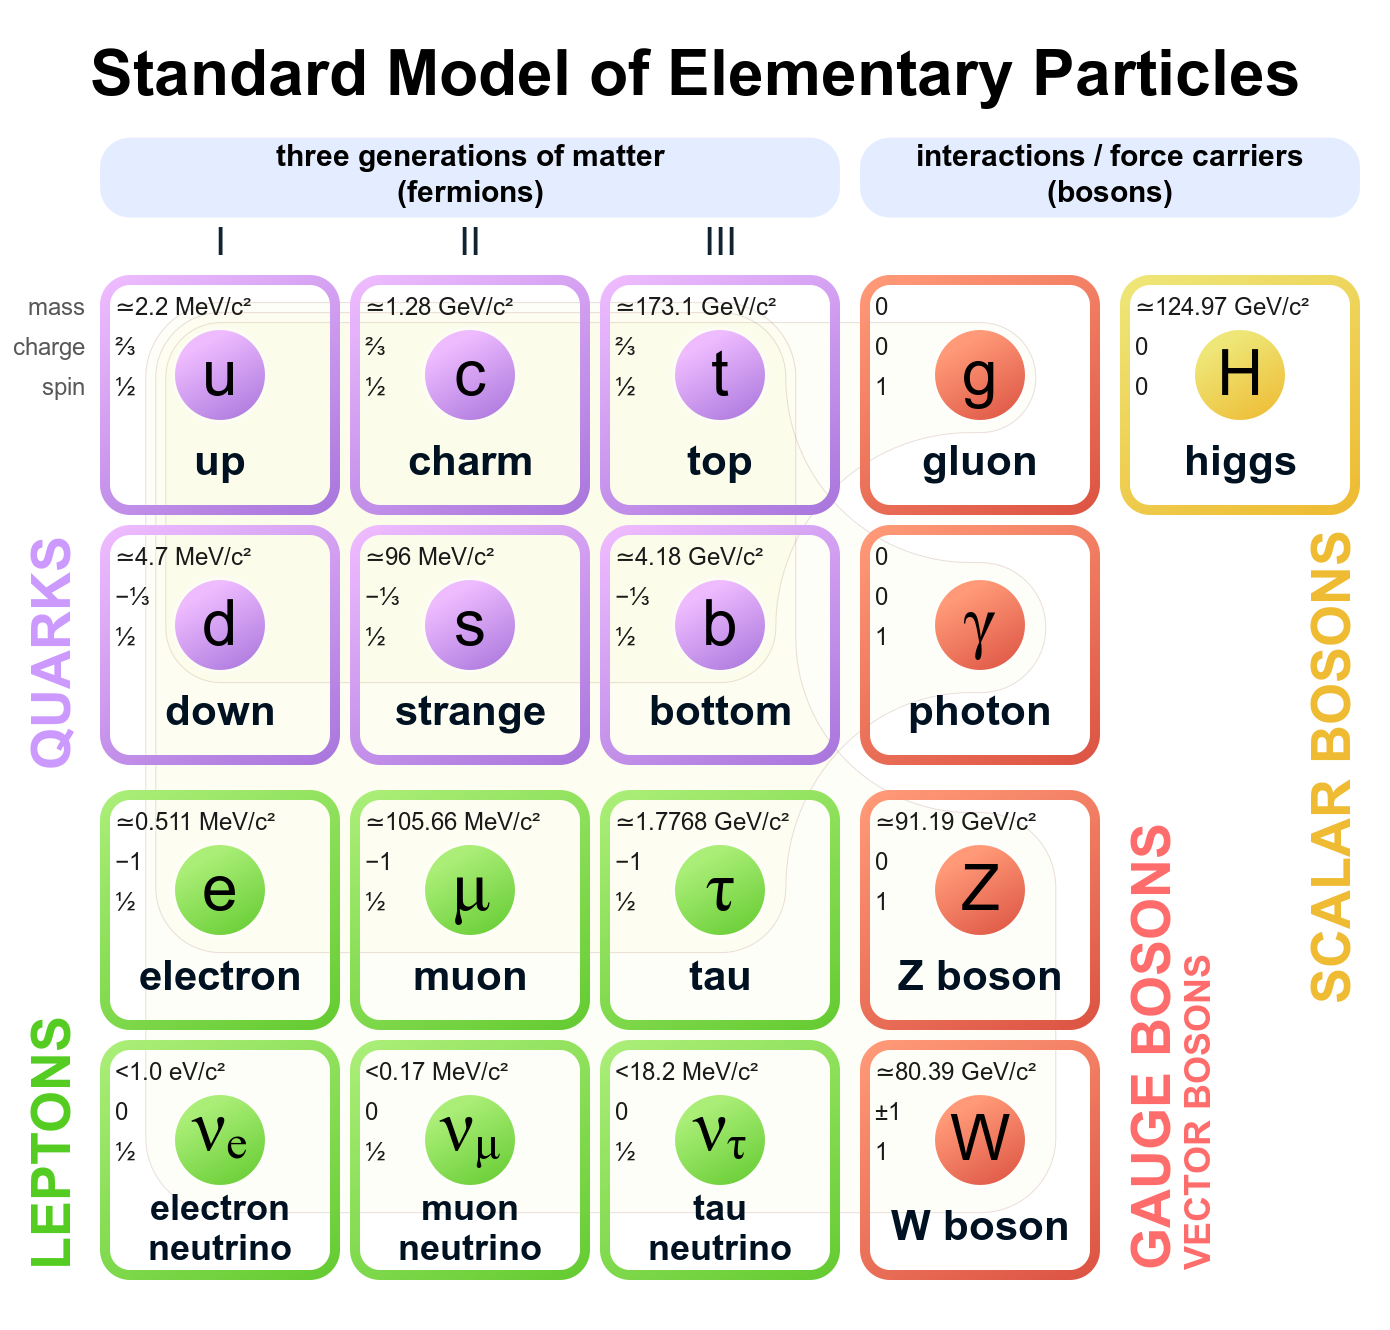
\includegraphics[width=0.65\textwidth]{fig/theory/Standard_Model_of_Elementary_Particles.png}
		\caption[Table of elementary particles in the SM. The leftmost three columns correspond to three generations of fermions, 
		the fourth column from the left shows the gauge bosons which mediate the elementary forces, and the rightmost column shows the Higgs boson. 
		For each particle, mass, charge, and spin are labeled, with mass values given as of 2019.]
		{Table~\cite{SMImage} of elementary particles in the SM. The leftmost three columns correspond to three generations of fermions, 
		the fourth column from the left shows the gauge bosons which mediate the fundamental forces, and the rightmost column shows the Higgs boson. 
		For each particle, mass, charge, and spin are labeled, with mass values given as of 2019.}
		\label{fig:SMParticles}
	\end{center}
\end{figure}

Figure \ref{fig:SMParticles} catalogs the elementary particles of the SM. These particles come in two broad types: fermions and bosons. Fermions are particles of half-integer spin that obey 
the Pauli exclusion principle. They are, therefore, responsible for the structure of matter. 
Each fermion has a corresponding antiparticle that has opposite electrical charge, but is otherwise identical. 
The fermions are subdivided into two types in three generations, the generations corresponding to mass.
Quarks are fermions that carry both fractional electric charge and color charge, so they participate in the electroweak and strong interactions. 
Leptons are fermions that carry integer electric charge and participate in the electroweak interaction.
In contrast to fermions, bosons have integer spin. The vector gauge bosons function as mediators of the fundamental forces of nature. 
The gluons mediate the strong force, the photon the electromagnetic force, and the W and Z bosons the weak force. 
Finally, the electrically neutral, scalar Higgs boson emerges due to electroweak symmetry breaking, described later in this section. The interaction of the Higgs 
with the other particles in the SM is responsible for particle masses. 
In the context of this thesis, which is a search for \hzg{}, the most relevant elementary particles are the Higgs boson, Z boson, leptons, and photon. 
Therefore, the remainder of this section will describe electroweak theory and the Higgs mechanism in more detail. Other aspects of the SM, such as quantum chromodynamics, 
are of importance in collider physics, but of less relevance for this specific search. Such topics are omitted in order to narrow the scope of the discussion.

\section{Electroweak Theory}
To motivate the Higgs mechanism and Higgs interactions, it is useful to first consider the electroweak interaction absent the Higgs. The electroweak piece of the 
SM Lagrangian can be written as 
\begin{align}
	& \mathcal{L}_{EW} = -\frac{1}{4}A_a^{\mu\nu}A^a_{\mu\nu} - \frac{1}{4}B^{\mu\nu}B_{\mu\nu} + i\sum_L \bar{L}\gamma^{\mu}D_{\mu,L}L + i\sum_R \bar{R}\gamma^{\mu}D_{\mu,R}R \label{eqn:LEWK}\\
	& A^a_{\mu\nu} = \partial_{\mu}A_{\nu}^{a} - \partial_{\nu}A_{\mu} + g\varepsilon_{abc}W^{b}_{\mu}W^{c}_{\nu} \\
	& B_{\mu\nu} = \partial_{\mu}B_{\nu} - \partial_{\nu}B_{\mu} \\
	& D_{\mu,L} = \partial_{\mu} + \frac{ig}{2}\tau\cdot A_{\mu} + \frac{ig'}{2}B_{\mu}Y \label{eqn:DL}\\
	& D_{\mu,R} = \partial_{\mu} + \frac{ig'}{2}B_{\mu}Y. \label{eqn:DR}
\end{align}
In the above equations, $A_{\mu\nu}^a$ represents an SU(2)$_L$ triplet of gauge fields and $B_{\mu\nu}$ represents a U(1) gauge field. The third and fourth terms in equation \ref{eqn:LEWK} 
describe the interactions of these gauge fields with the fermions, both quarks and leptons. Note that the interaction depends on the chirality of the fermions, where the left-handed 
fermions are denoted as $L$ and the right-handed as $R$. The right-handed fermions interact only with the U(1) field, while the left-handed fermions interact with the U(1) and SU(2)$_L$ fields. 
This is encoded by the derivative operators $D_{\mu,L}$ and $D_{\mu,R}$ defined in equations \ref{eqn:DL} and \ref{eqn:DR} in terms of the fields, Pauli matrices ($\tau$), hypercharge operator Y, and the couplings $g$ and $g'$. 

\section{Spontaneous Symmetry Breaking (Higgs Mechanism)}
One important property of the electroweak Lagrangian in equation \ref{eqn:LEWK} is that the bosons associated with the gauge fields are all massless. 
However, the direct observation of charged and neutral 
current interactions \cite{HASERT1973121,HASERT1973138} at CERN in 1973 implied that the W and Z boson must have relatively large masses in the range of 50--100\GeV. Indeed, the massive W and Z bosons were later discovered and measured \cite{UA1:1983crd,UA2:1983tsx} at the CERN Super Proton Synchroton in 1983. 
A solution to this shortcoming of the electroweak theory came in the form of the Higgs mechanism \cite{Englert:1964et,Higgs:1964ia,Higgs:1964pj},
which spontaneously breaks the SU(2)xU(1) gauge symmetry. One consequence of this is the addition of a real 
Higgs field accompanied by a massive Higgs boson. The W and Z boson masses arise naturally due to the electroweak symmetry breaking, 
while fermion masses are explained via additional Yukawa couplings to the Higgs boson. 
The discovery of the Higgs boson and subsequent measurements of its properties have provided experimental verification that the Higgs mechanism 
is a central piece of the Standard Model. 

To understand how the Higgs mechanism works, consider the introduction of a complex scalar field $\sf \Phi$, which 
transforms as a doublet under SU(2)$_L$.
\begin{equation}
    \label{eqn:higgsField}
    \Phi = 
    \begin{bmatrix}
        \phi^{+} \\ 
        \phi^{0}
    \end{bmatrix}
\end{equation}
Its contribution to the Lagrangian is given by:
\begin{equation}
    \mathcal{L_{H}} = (D^{\mu}_L\Phi)^{\dagger}(D_{\mu,L}\Phi) - V(\Phi)
    \label{LHiggs}
\end{equation}
where the Higgs potential takes the form
\begin{equation}
    V(\Phi) = \mu^{2}|\Phi^{\dagger}\Phi| + \lambda \Big(|\Phi^{\dagger}\Phi|\Big)^{2}.
    \label{VHiggs}
\end{equation}
Consider the case in which the parameters of the Higgs potential $\lambda$ and $\mu$ satisfy the conditions 
$\lambda > 0$ and $\mu^{2} < 0$. Then the shape of the potential is shown in Fig. \ref{fig:VHiggs} (right). There is no minimum of the 
potential at $\Phi = 0$. Rather, an infinite set of minima lie around a circle in the complex plane. Hence, it is said that $\Phi$ 
has a nonzero vacuum expectation value (VEV). The value of the VEV in terms of $\mu$ and $\lambda$ can be determined by explicitly
minimizing the potential:
\begin{align*}
    \frac{\partial}{\partial(\Phi^{\dagger}\Phi)}V(\Phi) &= 0 \\
    \mu^{2} + 2\lambda\Big(|\Phi^{\dagger}\Phi|\Big) &= 0 \\
    \mu^{2} + 2\lambda\Big[(\phi^{+})^{2} + (\phi^{0})^{2}\Big] &= 0 \numberthis
    \label{VHiggsMinimization}
\end{align*}
This can be minimized in many ways depending on individual values of $\phi^{+}$ and $\phi^{0}$ in the vacuum. By convention,
and without loss of generality, we choose the case in which $\phi^{+} = 0$. In this case we obtain the equation
\begin{equation}
    \phi^{0} = \sqrt{\frac{-\mu^{2}}{2\lambda}} = \frac{1}{\sqrt{2}}v
\end{equation}
where we have defined $v \equiv \sqrt{-\mu^{2}/\lambda}$.

\begin{figure}
	\begin{center}
	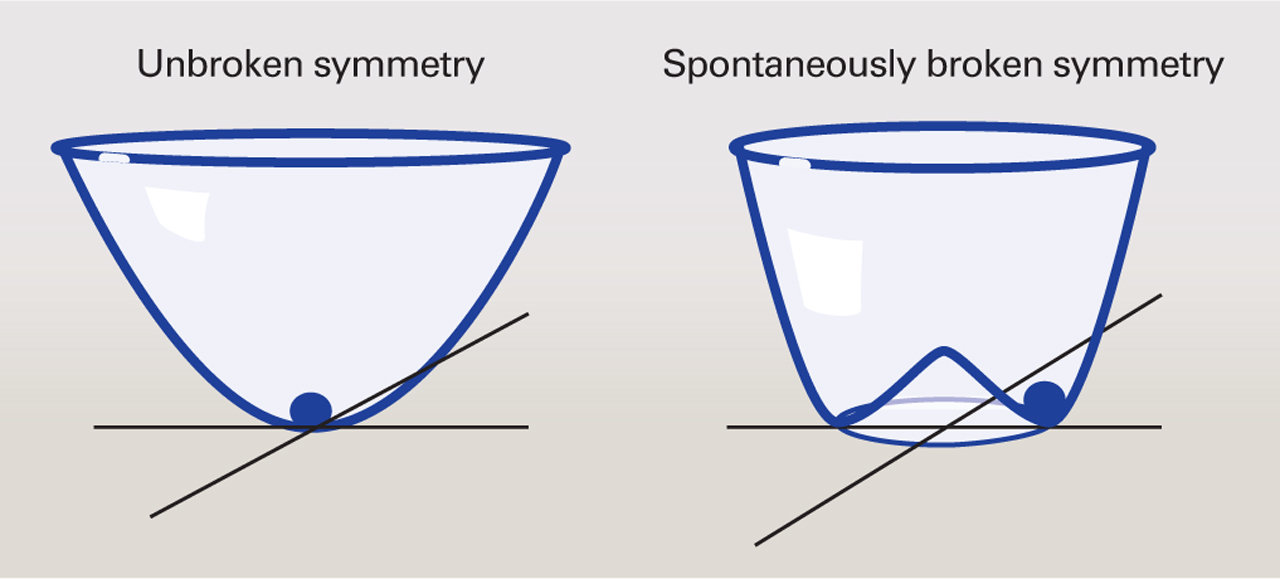
\includegraphics[width=0.75\textwidth]{fig/theory/spont_sym_breaking.jpg}
		\caption
		[Comparison of the shapes of complex scalar potentials without symmetry breaking (left) and with spontaneous symmetry breaking (right). 
		The transverse axes represent the real-imaginary $\Phi$ plane, 
		and the vertical axis represents the magnitude of the potential $V(\Phi)$. The diagram at right corresponds to the shape of the Higgs potential in the SM.]
		{Comparison of the shapes of complex scalar potentials without symmetry breaking (left) and with spontaneous symmetry breaking (right)~\cite{VHiggsImage}. 
		The transverse axes represent the real-imaginary $\Phi$ plane, 
		and the vertical axis represents the magnitude of the potential $V(\Phi)$. The diagram at right corresponds to the shape of the Higgs potential in the SM.}
		\label{fig:VHiggs}
	\end{center}
\end{figure}

The existence of the Higgs VEV has profound implications. To see this, it is helpful to reparameterize the scalar doublet field
$\Phi$ as follows:
\begin{equation}
    \Phi = \frac{1}{\sqrt{2}}e^{i\frac{\tau^{a}}{2}\theta_{a}(x)}
    \begin{bmatrix}
        0 \\
        v + h(x)
    \end{bmatrix}
    \label{reparamHiggsField}
\end{equation}
As $\Phi$ is invariant under local SU(2)$_L$ gauge transformations, the prefactor may be rotated away. This is equivalent to setting 
$\theta(x) = 0$ in equation \ref{reparamHiggsField}. This choice of gauge is known as the unitary gauge, and leads to 
\begin{equation}
    \Phi = \frac{1}{\sqrt{2}}
    \begin{bmatrix}
        0 \\
        v + h(x)
    \end{bmatrix}
    \label{HiggsFieldUnitaryGauge}
\end{equation}
Given the above form of $\Phi$, we can now evaluate the Higgs Lagrangian (equation \ref{LHiggs}), starting with the kinetic term
$(D^{\mu}_L\Phi)^{\dagger}(D_{\mu,L}\Phi)$.
\begin{align*}
    (D^{\mu}_L\Phi)^{\dagger}(D_{\mu,L}\Phi) &= \Big| (\partial_{\mu} - \frac{ig}{2}\tau\cdot A_{\mu} - \frac{ig'}{2}B_{\mu}Y)\Phi\Big|^{2} \\
    &= \frac{1}{2}
    \Big| 
    \begin{bmatrix}
        \partial_{\mu} - \frac{i}{2}(gA_{\mu}^{3} + g'B_{\mu}) & -\frac{ig}{2}(A_{\mu}^{1} - iA_{\mu}^{2}) \\
            -\frac{ig}{2}(A_{\mu}^{1} + iA_{\mu}^{2}) & \partial_{\mu} + \frac{i}{2}(gA_{\mu}^{3} - g'B_{\mu})
    \end{bmatrix} 
    \begin{bmatrix}
        0 \\ 
        v + h(x)
    \end{bmatrix} 
    \Big|^{2} \\ &=  
    \frac{1}{2}\Big| 
    \begin{bmatrix}
        -\frac{ig}{2}(A_{\mu}^{1} - iA_{\mu}^{2})(v + h(x)) \\
        \partial_{\mu}h(x) + \frac{i}{2}(gA_{\mu}^{3} - g'B_{\mu})(v + h(x))
    \end{bmatrix}
    \Big|^{2} \\ &= 
    \frac{1}{2}\partial_{\mu}h(x)\partial^{\mu}h(x) + \frac{1}{8}(gA_{\mu}^{3} - g'B_{\mu})(gA^{\mu}_{3} - g'B^{\mu})(v + h(x))^{2} \\ &+ 
    \frac{g^{2}}{8}(A_{\mu}^{1} - iA_{\mu}^{2})(A_{\mu}^{1} + iA_{\mu}^{2})(v + h(x))^{2} \label{kinHiggsExpansion} \numberthis 
\end{align*}
With some foreknowledge of the result, we define the physical gauge fields and their masses.
\begin{align}
    W_{\mu}^{\pm} &= \frac{1}{\sqrt{2}}(A_{\mu}^{1} \mp iA_{\mu}^{2}) \; &m_{W} = \frac{gv}{2} \\
    Z_{\mu} &= \frac{1}{\sqrt{g^{2} + g'^{2}}}(gA_{\mu}^{3} - g'B_{\mu}) \; &m_{Z} = \sqrt{g^{2} + g'^{2}}\frac{v}{2} \\
    A_{\mu} &= \frac{1}{\sqrt{g^{2} + g'^{2}}}(g'A_{\mu}^{3} + gB_{\mu}) \; &m_{A} = 0
    \label{gaugeBosonsAndMasses}
\end{align}
Then the kinetic term of the Higgs Lagrangian can be recast as
\begin{align*}
    (D^{\mu}_L\Phi)^{\dagger}(D_{\mu,L}\Phi) &= \frac{1}{2}\partial_{\mu}h(x)\partial^{\mu}h(x) \\ 
    &+ \frac{1}{2}m_{Z}^{2}Z_{\mu}Z^{\mu} + m_{W}^{2}W_{\mu}^{+}W^{-\mu} \\
    &+ \frac{v}{4}(g^{2} + g'^{2})Z_{\mu}Z^{\mu}h + \frac{1}{8}(g^{2} + g'^{2})Z_{\mu}Z^{\mu}h^{2} \\
    &+ \frac{v}{4}g^{2}W_{\mu}^{+}W^{-\mu}h + \frac{1}{8}g^{2}W_{\mu}^{+}W^{-\mu}h^{2} \label{kinHiggsMasses}\numberthis
\end{align*}
Equation \ref{kinHiggsMasses} provides a great deal of information on the physical ramifications of the Higgs mechanism.
The first term is the kinetic term of the physical Higgs boson field. The second and third terms are the mass terms of the Z and W 
bosons, respectively. The fourth and fifth terms show the linear and quadratic couplings of the Z boson to the Higgs boson, respectively.
Finally, the sixth and seventh terms show the linear and quadratic couplings of the W boson to the Higgs boson, respectively. 
Given the form of equation \ref{HiggsFieldUnitaryGauge}, a similar expansion can be carried out on the Higgs potential
(equation \ref{VHiggs}). Here, the terms involving the physical Higgs boson are most interesting, so constant terms are dropped.
\begin{align*}
    V(\Phi) &= \frac{\mu^{2}}{2}(v+h)^{2} + \frac{\lambda}{4}((v+h)^{2})^{2} \\
    &\rightarrow \lambda v^{2}h^{2} + \lambda vh^{3} + \frac{\lambda}{4}h^{4} \label{expandedVHiggs} \numberthis
\end{align*}
The first term is a Higgs mass term, with $m_{H} = \sqrt{2\lambda v^{2}}$. The second and third terms describe the Higgs 
trilinear and quartic self-couplings, respectively.

The Lagrangian including the Higgs doublet $\Phi$ can be further extended to incorporate interactions between the Higgs and fermion fields. These interactions, along with the nonzero Higgs VEV, provide a mechanism to generate the fermion masses. The interactions take the 
form of Yukawa couplings:
\begin{equation}
    \mathcal{L}_{Yukawa} = Y_{ij}^{d}\bar{Q}^{i}_{L}\Phi d_{R}^{j} + Y_{ij}^{u}\bar{Q}^{i}_{L}\tilde{\Phi} u_{R}^{j} 
    + Y_{ij}^{e}\bar{L}^{i}_{L}\Phi e_{R}^{j} + h.c.,
    \label{LYukawa}
\end{equation}
where $\tilde{\Phi} \equiv i\tau_{2}\Phi^{*}$, and $u$, $d$, and $e$ represent up-type quarks, down-type quarks, and leptons, respectively. The constants $Y_{ij}^a$ denote the Yukawa couplings in each case, $Q^i$ is the set of SU(2) quark doublets, and $L^i$ is the set of SU(2) lepton doublets.
\begin{equation}
    \tilde{\Phi} \equiv i\tau_{2}\Phi^{*}
    \label{PhiDual}
\end{equation}
Plugging in the unitary gauge parameterization of equation \ref{HiggsFieldUnitaryGauge}, this evaluates to 
\begin{align}
    \mathcal{L}_{Yukawa} = \frac{Y_{ij}^{d}}{\sqrt{2}}\bar{d}_{L}^{i}(v + h)d_{R}^{j} 
    + \frac{Y_{ij}^{u}}{\sqrt{2}}\bar{u}_{L}^{i}(v+h)u_{R}^{j} + \frac{Y_{ij}^{e}}{\sqrt{2}}\bar{e}_{L}^{i}(v+h)e_{R}^{j}
    \label{expandedLYuk}
\end{align}
It is worth looking closely at the terms in equation \ref{expandedLYuk}. For a given fermion type, the first term in the parentheses
is a fermion mass term. The second term in the parentheses gives the coupling of the fermion to the Higgs boson. With this in mind, 
we observe that the fermion mass is given in terms of the couplings and the Higgs vev by 
\begin{equation}
    m_{f} = \frac{y_{f}v}{\sqrt{2}}
    \label{fermionMass}
\end{equation}
where $y_{f}$ is the relevant value taken from the Yukawa coupling matrix. In addition, we see that the strength of the fermion coupling
to the Higgs boson is given by $\frac{m_{f}}{v}$. Thus, fermions couple to the Higgs boson with strength directly proportional 
to their masses. This result has important consequences in the context of collider experiments, as it regulates the rates of
Higgs production and decay related to each fermion-Higgs interaction. 

%The existence of the Higgs VEV leads naturally to the masses of the W and Z bosons. This can be shown by squaring the covariant 
%derivative acting on the scalar doublet $\Phi$ and evaluating the result in the vacuum. Note that in the vacuum, all terms involving 
%the partial derivative $\partial_{\mu}$ will yield zero contribution. Therefore, keeping only the relevant terms, the squared covariant 
%derivative reduces to
%\begin{equation}
%    |D_{\mu}|^{2} \rightarrow (\frac{g}{2}A_{\mu}^{a}\tau^{a} +\frac{g'}{2}B_{\mu})(\frac{g}{2}A^{b\mu}\tau^{b} + \frac{g'}{2}B^{\mu})
%    \label{covDerivSquared}
%\end{equation}
%Evaluating this in the vacuum yields
%\begin{align}
%    \Delta\mathcal{L} &= \frac{1}{2}
%    \begin{bmatrix}0 & v
%    \end{bmatrix}
%    (\frac{g}{2}A_{\mu}^{a}\tau^{a} +\frac{g'}{2}B_{\mu})(\frac{g}{2}A^{b\mu}\tau^{b} + \frac{g'}{2}B^{\mu}) 
%    \begin{bmatrix}
%        0 \\ 
%        v
%    \end{bmatrix} \\ 
%    \Delta\mathcal{L} &=
%    \frac{1}{2}\frac{v^{2}}{4}[g^{2}(A_{\mu}^{1})^{2} g^{2}(A_{\mu}^{2})^{2} + (g'B_{\mu} - gA_{\mu}^{3})^{2}]
%\end{align}
%From this, we can identify the fields and masses for the positively and negatively charged W bosons and the neutral Z boson and photon. 
%These are as follows:


\section{Higgs Production}

At a hadron collider like the LHC, the Higgs boson can be produced via several different mechanisms, each mechanism occuring at a certain rate. The dominant production 
mechanism is gluon-gluon fusion (ggH), followed by vector boson fusion (VBF) production, which is about an order of magnitude rarer. Less common production mechanisms, but 
still relevant for a search at the LHC, are the associated production mechanisms WH, ZH, and t$\bar{t}$H. The cross sections for each Higgs production mechanism as a function of 
center of mass energy are shown in Fig. \ref{fig:higgs_prod}.

\begin{figure}
	\begin{center}
	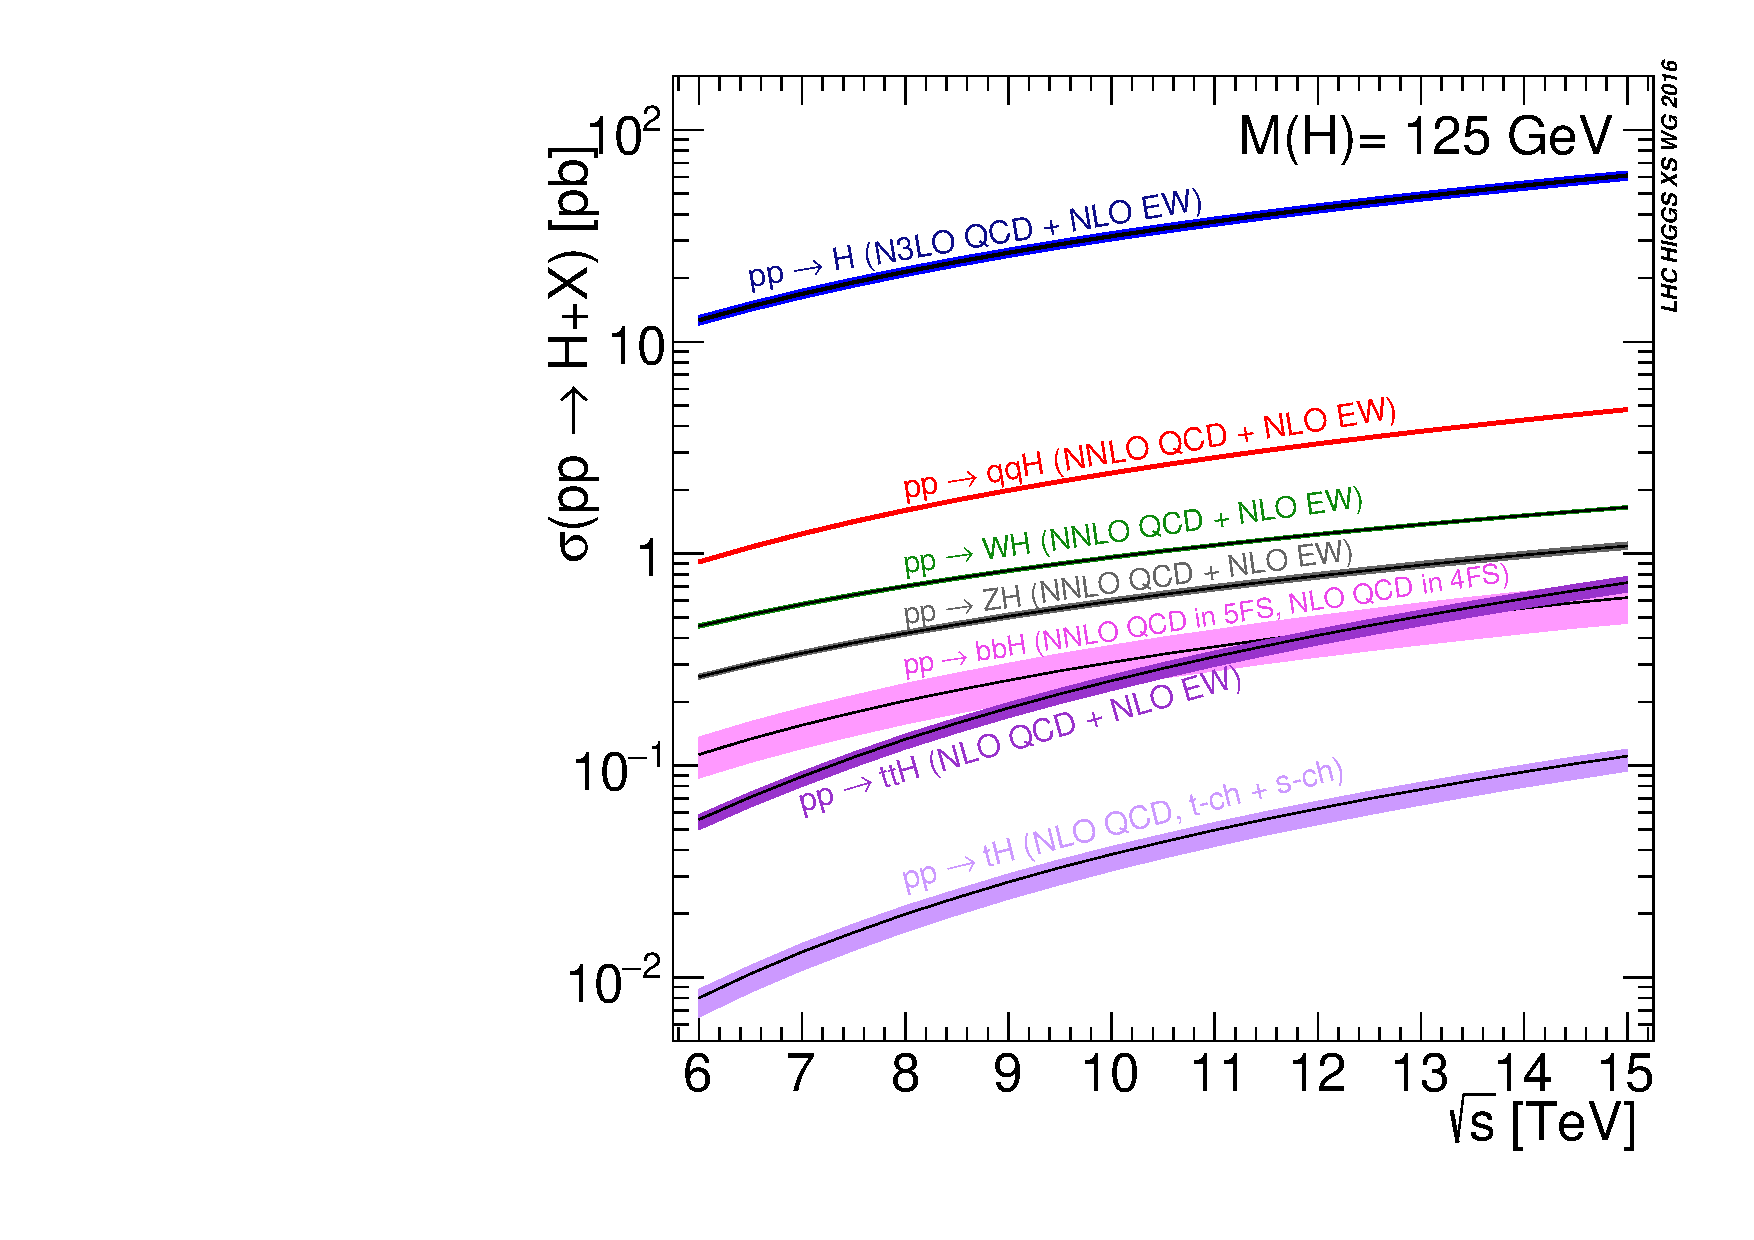
\includegraphics[width=0.75\textwidth]{fig/theory/Plot_Escan_H125_new_sqrt.pdf}
	\caption{Cross sections for different Higgs boson production mechanisms as a function of center of mass energy.}
	\label{fig:higgs_prod}
	\end{center}
\end{figure}

\section{Higgs Decay}

The Higgs boson decays rapidly after it is produced at the LHC. It can decay into a variety of final states, each occuring at a certain rate. Tree-level Higgs decays occur at rates 
proportional to the square of the mass of the decay products. Decays to b$\bar{b}$, WW, $\tau^+\tau^-$, and ZZ, are among the most common and experimentally accessible at the LHC. Other Higgs decays 
occur at loop-level, including $\PH \to \Pg\Pg$ and \hzg. Figure \ref{fig:higgs_br} shows the branching fractions at $\sqrt{s}=13$\TeV for different decay channels as a function of Higgs boson mass. 
We see that the branching fraction of \hzg is suppressed relative to several other production modes, so a search for \hzg must rely on the clean $\ell^+\ell^-\gamma$ signature.

\begin{figure}
	\begin{center}
	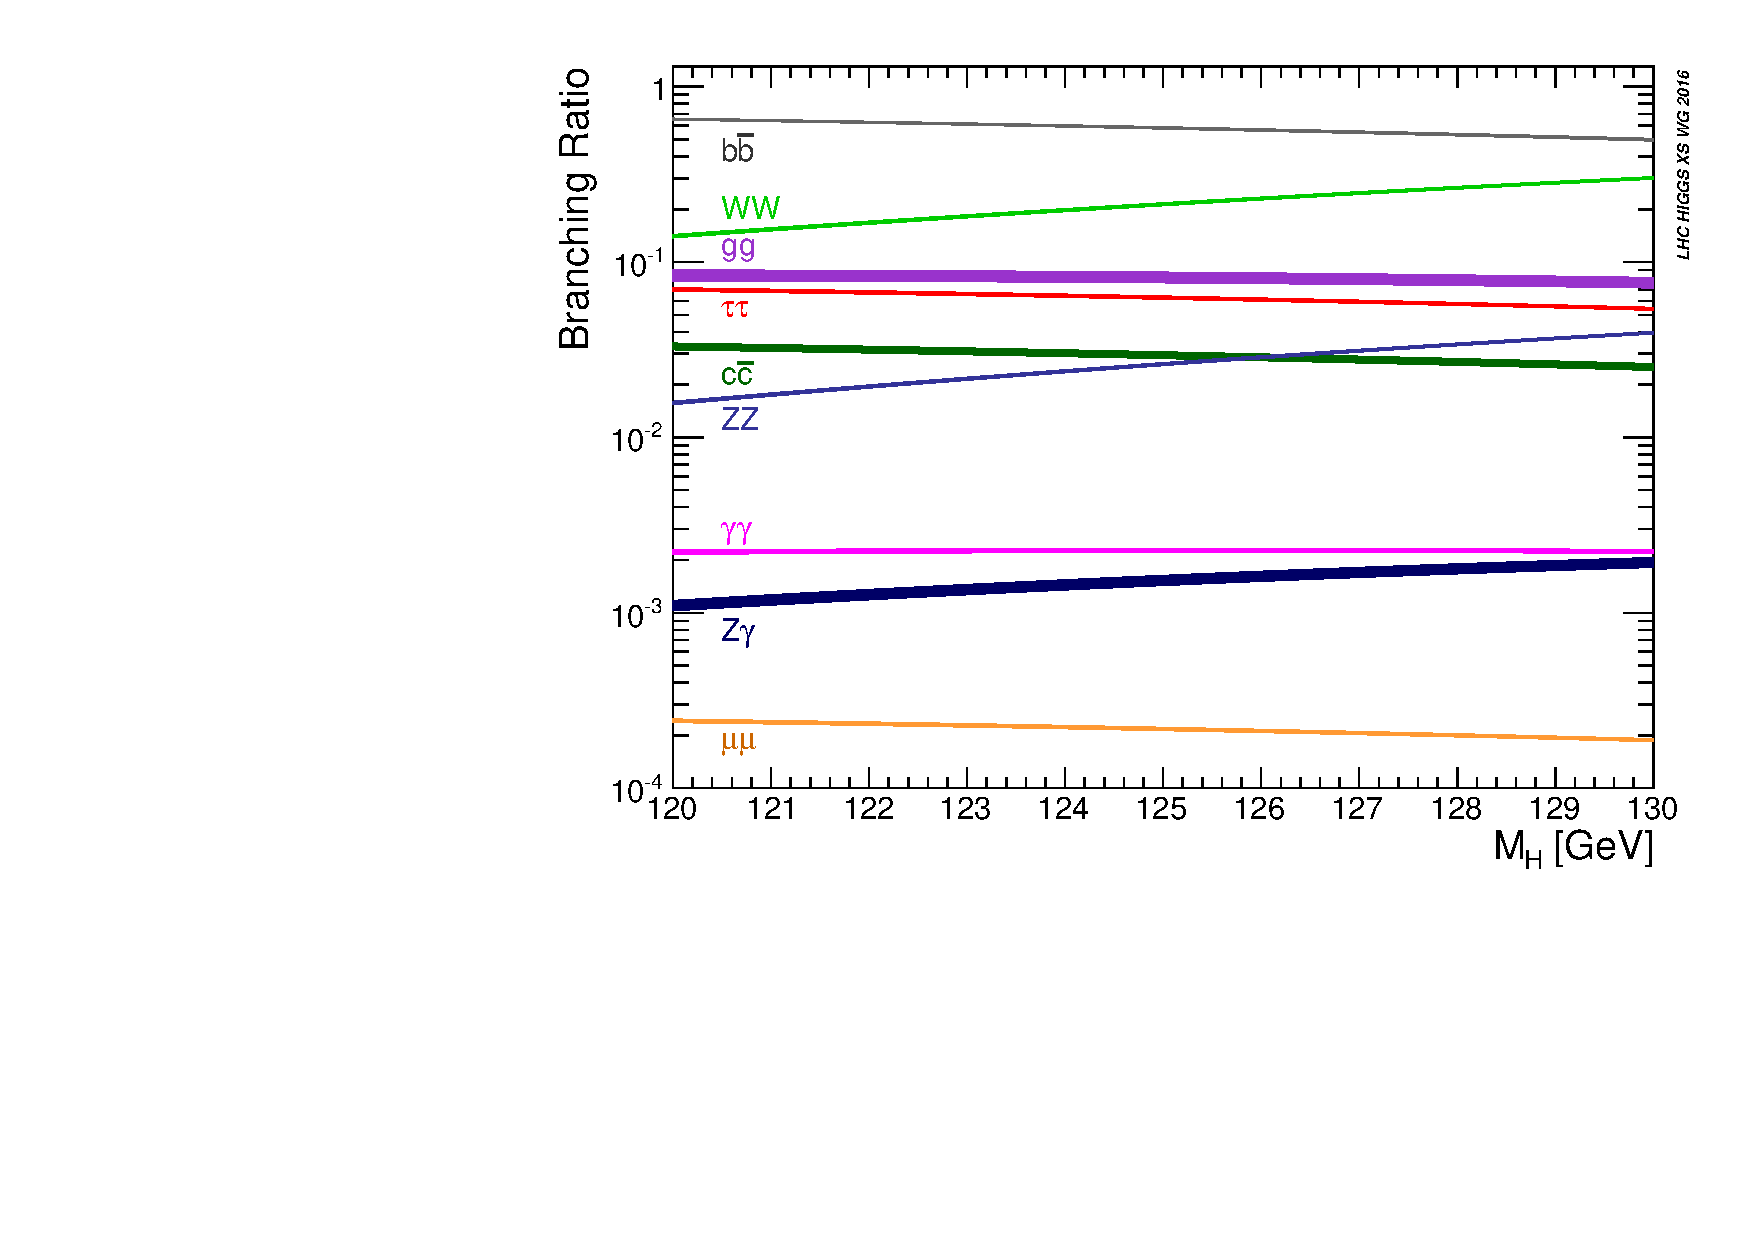
\includegraphics[width=0.75\textwidth]{fig/theory/SMHiggsBR.YR4-rect.pdf}
		\caption{Branching fraction of \hzg decay as a function of Higgs boson mass.}
		\label{fig:higgs_br}
	\end{center}
\end{figure}

\section{Physics Beyond the Standard Model}

One of the goals of the LHC is to search for BSM physics. While the decay \hzg{} is predicted in the SM, searching for it and measuring its branching fraction can indirectly probe potential 
new physics phenomena. A few unique features of \hzg{} make it well-suited as a BSM probe. First, the decay is loop-induced, which means that the introduction of new particles will contribute 
to the loop, interfering and altering the final branching fraction. Secondly, the decay \hgg{} is a very similar loop-induced process that has been discovered and measured extensively 
by the CMS and ATLAS Collaborations [REFS]. This means any new particle content entering into the \hzg{} loop will also enter into the \hgg{} loop. However, in the case of \hzg{}, the
Z boson couples to loop particles according to the SU(2)xU(1) quantum number rather than just the electric charge, as is the case for \hgg{}. 
It follows that potential BSM physics scenarios can shift the 
branching fractions of \hzg{} and \hgg{} by differing amounts, making the ratio $\mathcal{B}(\PH\rightarrow\PZ\gamma)/\mathcal{B}(\PH\rightarrow\gamma\gamma)$ a sensitive observable. In the SM, 
$\mathcal{B}(\PH\rightarrow\PZ\gamma)/\mathcal{B}(\PH\rightarrow\gamma\gamma) = 0.69 \pm 0.04$. A measurement of a significant deviation from this value would be an indicator of possible BSM physics.
Below, we describe a few examples of BSM scenarios that can affect this ratio.

One way to consider BSM effects in the context of \hzg{} is to introduce new particles, like a W' boson, charged scalar, or a pair of charged leptons. 
This is the approach taken by Carena, Low, and Wagner~\cite{Zg_theory_decaywidth}. The W' possibility is motivated by the fact that the W boson loop is the dominant 
contribution in the SM. The W' can be defined by an SU(2) triplet and characterized by mass and Higgs coupling parameters. Figure \ref{fig:rzg_bsm} (left) shows contours of constant branching fraction 
enhancement in the \hzg{} and \hgg{} decay channels in the mass-coupling plane for the W' model. 
Depending on the parameter values, the level of enhancement can be up to double the SM value, and it differs 
significantly in the two channels. Similarly, we can imagine a new charged scalar or a pair of new charged leptons. The branching fraction enhancement contour plots in Fig. \ref{fig:rzg_bsm} show that for similar regions in the mass-coupling plane, \hzg{} can be enhanced, while \hgg{} is simultaneously diminished. 

Other relevant BSM physics models include extended Higgs sectors. Such models often contain charged Higgs bosons, which enter into the \hzg{} and \hgg{} loops and impact the branching fractions. 
In Ref. \cite{Zg_theory_extension}, Chiang and Yagyu catalog extended Higgs models of varying types: models with one singly-charged boson, those with one singly-charged and one doubly-charged boson, 
and those with two singly-charged bosons. In total, the authors consider thirteen models, including the two Higgs doublet model, the minimal SUSY model, and the Higgs triplet model. 
Figure \ref{fig:exthiggs} gives the ratio of decay widths $\Gamma(\PH\rightarrow\PZ\gamma)/\Gamma(\PH\rightarrow\gamma\gamma)$ as a function of the mass coefficient of the additional scalar field(s) for seven of the models. It is evident that, for mass scales accessible at the LHC, the ratio can be significantly shifted relative to the SM expectation. 


\begin{figure}[tb]
	\begin{center}
		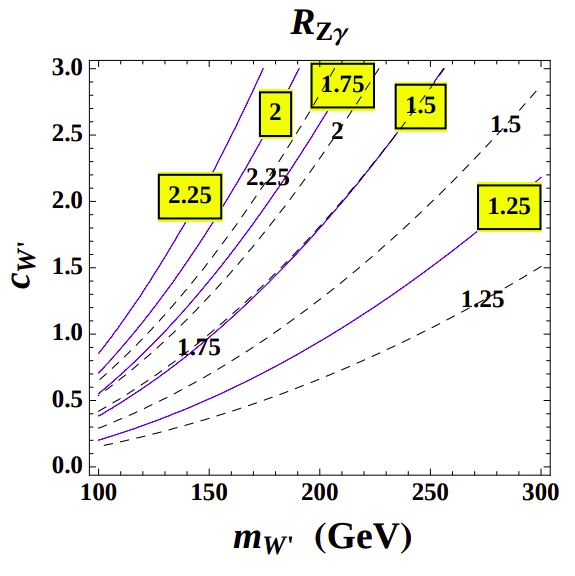
\includegraphics[width=0.30\textwidth, height=.30\textwidth]{fig/theory/rzgamma_wprime.png}
		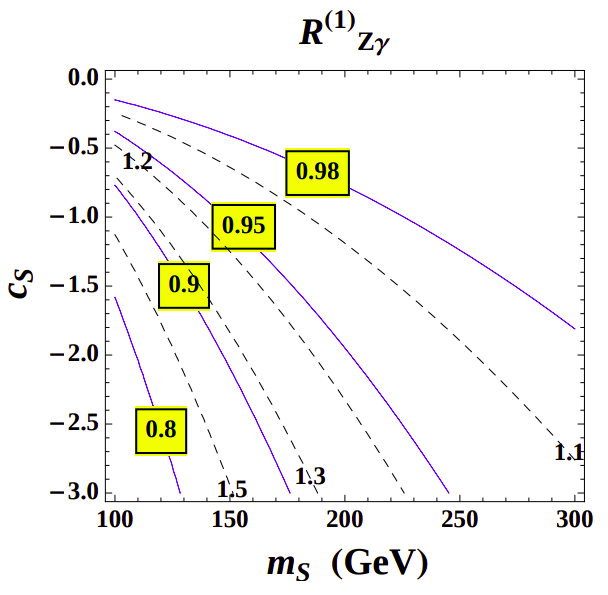
\includegraphics[width=0.30\textwidth, height=.30\textwidth]{fig/theory/rzgamma_scalar.png}
		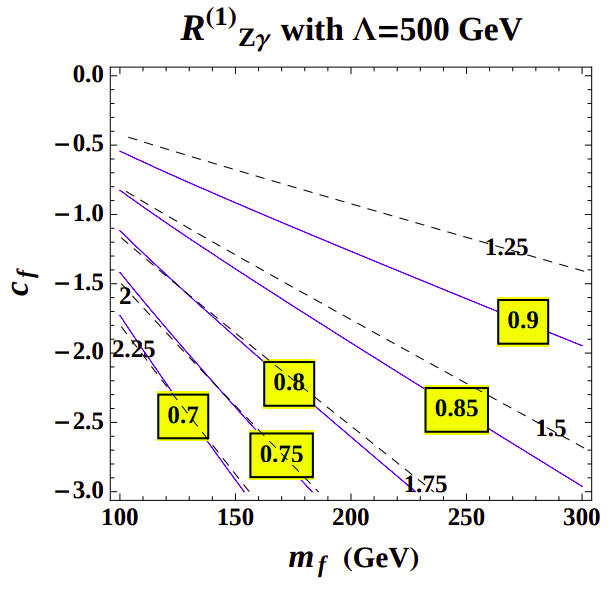
\includegraphics[width=0.30\textwidth, height=.30\textwidth]{fig/theory/rzgamma_fermion.png}
		\caption[Contours of constant branching fraction enhancement relative to the SM for the W' (left), charged scalar (center), 
		and charged lepton (right) scenarios. 
		The solid lines represent contours of enhancement in $\mathcal{B}$(\hzg), while the dashed lines correspond to \hgg{}. The yellow boxed numbers label the enhancement for each 
		\hzg{} contour, and the unboxed numbers label the enhancement for each \hgg{} contour.]
		{Contours of constant branching fraction enhancement relative to the SM for the W' (left), charged scalar (center), 
		and charged lepton (right) scenarios~\cite{Zg_theory_decaywidth}. 
		The solid lines represent contours of enhancement in $\mathcal{B}$(\hzg), while the dashed lines correspond to \hgg{}. The yellow boxed numbers label the enhancement for each 
		\hzg{} contour, and the unboxed numbers label the enhancement for each \hgg{} contour.}
		\label{fig:rzg_bsm}
	\end{center}
\end{figure}

\begin{figure}[tb]
	\begin{center}
		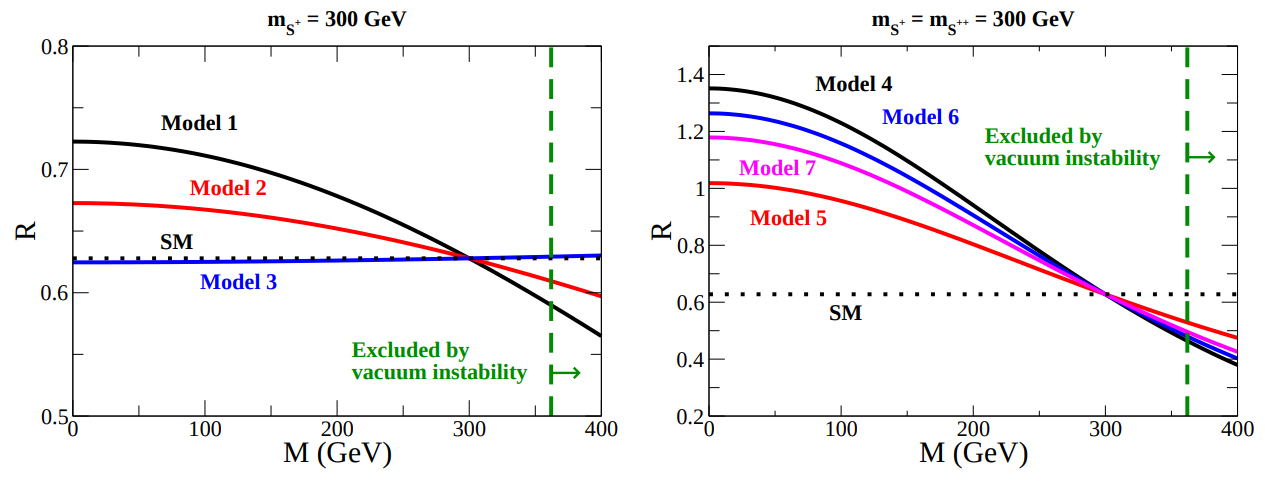
\includegraphics[width=0.9\textwidth]{fig/theory/rzgamma_exthiggs.png}
		\caption[Ratio of decay widths $\Gamma(\PH\rightarrow\PZ\gamma)/\Gamma(\PH\rightarrow\gamma\gamma)$ as a function of the mass coefficient of the additional scalar field(s) for 
		seven BSM models with extended Higgs sectors. 
		The models plotted on the left correspond to one additional singly-charged boson, and those on the right to one additional singly-charged and one additional doubly-charged boson.]
		{Ratio of decay widths $\Gamma(\PH\rightarrow\PZ\gamma)/\Gamma(\PH\rightarrow\gamma\gamma)$ as a function of the mass coefficient of the additional scalar field(s) for 
		seven BSM models with extended Higgs sectors~\cite{Zg_theory_extension}. 
		The models plotted on the left correspond to one additional singly-charged boson, and those on the right to one additional singly-charged and one additional doubly-charged boson.}
		\label{fig:exthiggs}
	\end{center}
\end{figure}


\chapter{Experiment Description}\label{sec:experiment}

\section{The Large Hadron Collider}
The Large Hadron Collider (LHC)~\cite{Evans_2008} is a high energy pp collider that serves several modern particle physics detector experiments. 
Built at CERN, straddling the French-Swiss border, and turned on for operation in 2008, it is the most powerful particle collider in history. 
The LHC was designed to collide protons at a maximum center of mass energy of $\sqrt s = 14\TeV$ 
with a maximum instantaneous luminosity of $10^{34}\cm^{-2}\mathrm{s}^{-1}$. To achieve this performance, the 27 km tunnel 
originally constructed for the Large Electron-Positron Collider (LEP)~\cite{Myers:226776} was repurposed to separately 
accelerate two counterrotating proton beams. The separate acceleration of the beams is made possible by oppositely oriented 
magnetic dipole fields in the two rings. When the beams achieve the desired energy, they are collided at one of four interaction points. 

The protons collided in the LHC are first gathered, bunched, and accelerated in other parts of the CERN accelerator complex before injection into the LHC ring. A detailed description of the injection chain can be found in Ref.~\cite{Benedikt:2004wm}, and a short summary is provided below. 
First, protons are stripped off of hydrogen atoms by a duoplasmatron and accelerated to 50\MeV by a linear accelerator (LINAC). Next, the protons are further accelerated 
in a series of synchroton rings of increasing size, the Proton Synchroton Booster (PSB), Proton Synchroton (PS), and Super Proton Synchroton (SPS). The SPS brings the 
proton beam energy up to 450\GeV. At this point, the beam is injected to the two LHC rings to be accelerated up to the final collision energy. Acceleration in the main 
ring is achieved by a system of thousands of superconducting dipole magnets, along with hundreds of correcting quadrupole magnets. A liquid helium cooling system is 
used to maintain the magnets at cryogenic temperatures. A full diagram of the CERN accelerator complex~\cite{CERN_complex}, including the parts relevant for the LHC, is shown in Fig. \ref{fig:accelerator_complex}.

\begin{figure}[tb]
  \centering
   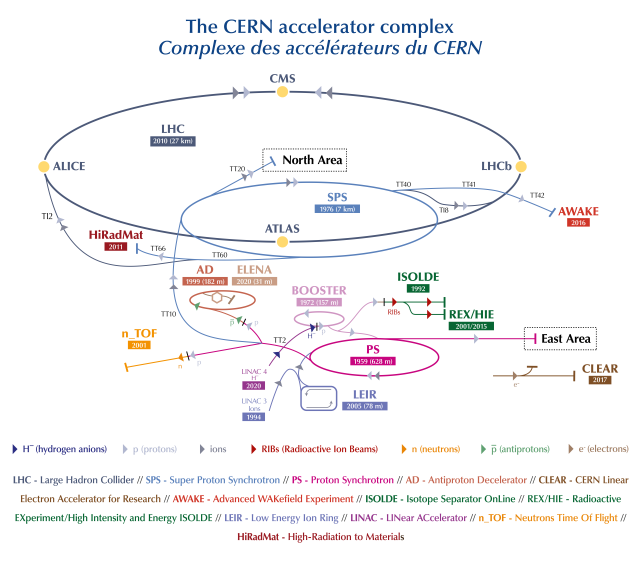
\includegraphics[width=0.9\textwidth]{fig/experiment/CCC-v2019-final-white.png}
	\caption[CERN accelerator complex.]{CERN accelerator complex~\cite{CERN_complex}.}
	\label{fig:accelerator_complex}
\end{figure}


\section{The Compact Muon Solenoid}
The CMS apparatus~\cite{CMS:2008xjf} is a multipurpose, nearly hermetic detector, designed to trigger on~\cite{CMS:2020cmk,CMS:2016ngn} and identify photons, electrons, muons, and (charged and neutral) hadrons~\cite{CMS:2015myp,CMS:2015xaf,CMS:2018rym,CMS:2014pgm}.
The central feature of the CMS apparatus is a superconducting solenoid of 6\unit{m} internal diameter, providing a magnetic field of $3.8$\unit{T}. Within the solenoid volume are a silicon pixel and strip tracker, a lead tungstate crystal electromagnetic calorimeter (ECAL), and a brass and scintillator hadron calorimeter (HCAL), each composed of a barrel and two endcap sections. The ECAL consists of 75,848 lead tungstate crystals, which provide coverage in pseudorapidity $\abs{\eta} < 1.48 $ in a barrel region (EB) and $1.48 < \abs{\eta} < 3.0$ in two endcap regions (EE). Preshower detectors consisting of two planes of silicon sensors interleaved with a total of $3$ radiation lengths of lead are located in front of each EE detector. Forward calorimeters extend the pseudorapidity coverage provided by the barrel and endcap detectors. Muons are measured in gas-ionization detectors embedded in the steel flux-return yoke outside the solenoid. Figure \ref{fig:detector} shows a schematic diagram of the CMS detector, and a more detailed description of the individual detector components and detector operation is provided below. 
%A more detailed description of the CMS detector, together with a definition of the coordinate system used and the relevant kinematic variables, can be found in Ref.~\cite{CMS:2008xjf}.

\begin{figure}[tb]
  \centering
   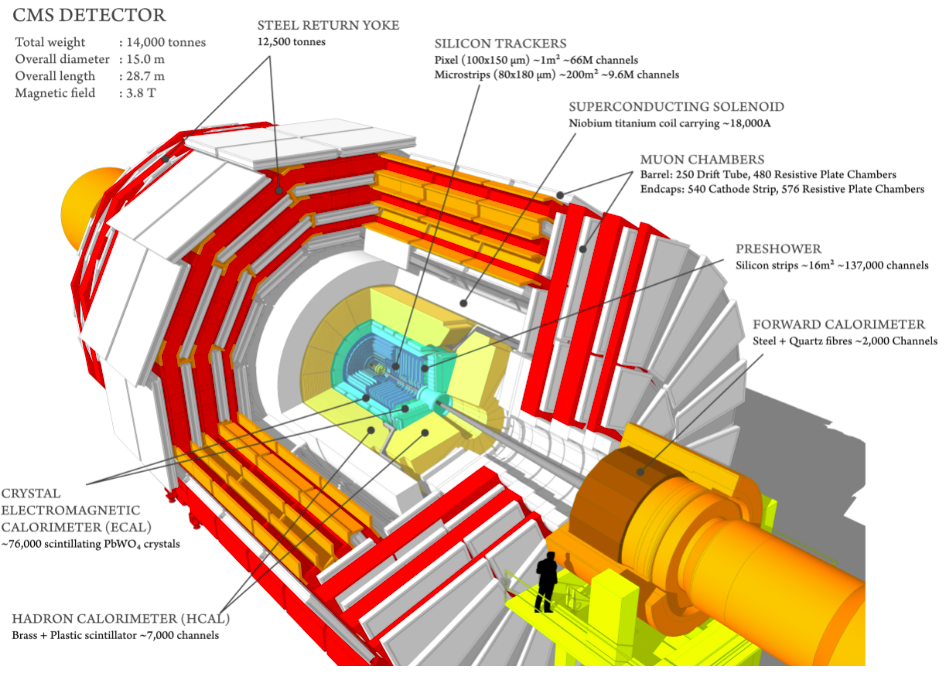
\includegraphics[width=0.75\textwidth]{fig/experiment/detector/cms_about_detector.png}
	\caption[CMS detector apparatus.]{CMS detector apparatus.~\cite{detector_image}}
	\label{fig:detector}
\end{figure}


\subsection{Superconducting Magnet}
The function of the superconducting magnet within the CMS detector is to bend the trajectories of charged particles. This is crucial for accurate particle identification and momentum measurement. 
Designed to provide a maximum magnetic field of $4$\unit{T}, its operating strength during pp collision runs is set to $3.8$\unit{T}. The bulk of the magnet is composed of NbTi, cooled by 
liquid helium to 4.5K, which is below the critical temperature for superconductivity. The magnet has a length of 12.5m, diameter of 6.3m, and mass of 220 tons. The solenoid encloses 
several detector components, including the tracker and the majority of the calorimeters. A steel flux-return yoke is built around the solenoid, and is composed of 5 wheels and two endcaps weighing 
a total of roughly 10,000 tons. 

\subsection{Inner Tracking System}
The inner tracking system is designed to reconstruct charged particle trajectories and vertices arising from particle decays. Comprised of a silicon pixel detector and silicon strip tracker, 
it covers the pseudorapidity region $|\eta| < 2.5$ and is designed for efficient and precise measurement of charged particles with transverse momentum (\pt) above about 1\GeV. 
At the LHC design luminosity for pp collisions, each bunch crossing leads to about 1,000 hits in the inner tracking system. As such, the inner tracking system was designed to be 
maximally radiation tolerant. 

The silicon pixel detector covers the inner region of $r < 10 \cm$. It is composed of $100 \times 150 \micron^{2}$ pixels, arranged in three barrel layers and two endcap disks. Due to the extreme 
radiation environment, the innermost layer was designed to be replaced after about two years of LHC operation. 
In response to LHC running conditions and detector degradation, a replacement and upgrade of the full pixel detector was made during the LHC extended year-end technical stop in 2016--2017. 

The silicon strip tracker covers the region $20 < r < 116 \cm$. It is divided into three subsystems: the Tracker Inner Barrel (TIB), Tracker Inner Disks (TID), and Tracker Outer Barrel (TOB). 
The strip thickness is $320 \micron$ ($500 \micron$) in the TIB/TID (TOB). A schematic diagram of the CMS inner tracking system in the r-z plane is shown in Fig. \ref{fig:cms_tracker}.

\begin{figure}[tb]
  \centering
   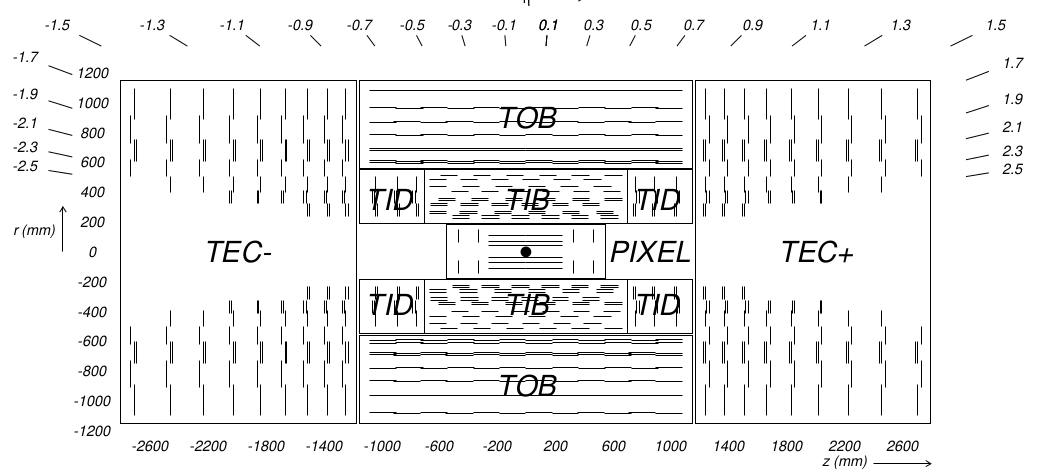
\includegraphics[width=0.8\textwidth]{fig/experiment/detector/cms_tracker.png}
	\caption[Cross section of the CMS inner tracking system in the r-z plane.]{Cross section of the CMS inner tracking system in the r-z plane.~\cite{CMS:2008xjf}}
	\label{fig:cms_tracker}
\end{figure}


\subsection{Electromagnetic Calorimeter (ECAL)}
The electromagnetic calorimeter (ECAL) is designed to identify and measure electromagnetic particles by inducing and characterizing electromagnetic showers. 
It is made up of 61,200 lead tungstate (PbWO$_4$) crystals in the barrel (EB), which covers $|\eta| < 1.479$, plus 7,324 crystals in each endcap (EE), which cover the range $1.479 < |\eta| < 3.0$. A preshower system lies in front of the EE. The preshower is a lead and silicon sampling calorimeter designed to aid in the identification of neutral pions and to improve the spatial resolution in the 
endcap region. 
The crystal length corresponds to 25.8 (24.7) radiation lengths in the EB (EE). When electromagnetic particles, such as 
electrons and photons, encounter the ECAL and interact with the crystal material, electromagnetic showers are induced. 
Light is emitted by the ECAL crystals proportional to the energy of constituent particles in the shower, allowing 
for reconstruction of the shower energy. An array of fast and radiation-tolerant photodetectors detects the emitted light, and this information is saved off detector. 
For this purpose, the EB uses avalanche photodiodes, while the EE uses vacuum phototriodes. As shown in Fig. \ref{fig:cms_ecal_response}, the ECAL has maintained good performance with minimal degradation throughout the duration of Run 1 and Run 2 of the LHC.

\begin{figure}[tb]
  \centering
   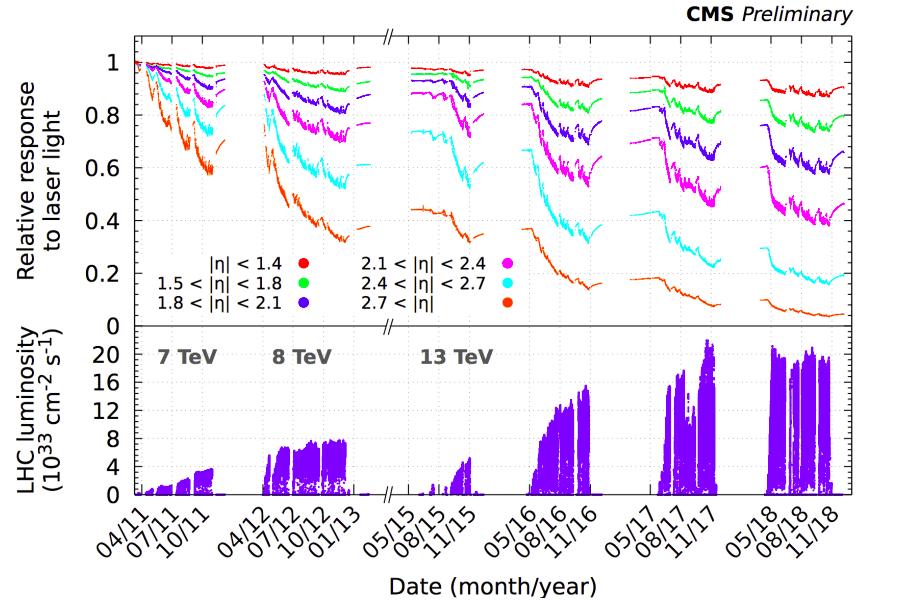
\includegraphics[width=0.8\textwidth]{fig/experiment/detector/cms_ecal_response.png}
	\caption[Response of the CMS ECAL crystals to injected laser light as a function of time, broken into regions of $|\eta|$.]
	{Response of the CMS ECAL crystals to injected laser light as a function of time, broken into regions of $|\eta|$~\cite{Cavallari:2798128}.}
	\label{fig:cms_ecal_response}
\end{figure}

\subsection{Hadronic Calorimeter (HCAL)}
Measurements of hadrons, jets, and missing transverse momentum are crucial at a hadron collider like the LHC. The CMS hadronic calorimeter (HCAL) is instrumental in such 
measurements. The HCAL is primarily a sampling calorimeter broken into several subdetectors. The barrel (HB) covers the range $|\eta| < 1.3$, the endcaps (HE) cover the range $1.3 < |\eta| < 3$, the forward calorimeter (HF) covers the range $3 < |\eta| < 5$, and an outer barrel calorimeter (HO) covers $|\eta| < 1.3$ outside of the solenoid magnet. 

Layers of brass absorber are interleaved with plastic scintillator in the HB and HE, with a total absorber thickness of 5.82--10.6 interaction lengths in the HB and about 10 interaction lengths in the HE. Scintillation light emitted by the active material is measured and transmitted off detector using hybrid photodiodes.
The design of the HF was motivated by the extreme particle fluxes in the very forward region. The HF is made up of steel plate absorbers, in which quartz fibers are inserted to serve as the active material. Cherenkov light is produced when shower particles moving at speeds above the Cherenkov threshold 
pass through the fibers, and a calculable fraction of the light is captured by the fibers. The function of the HO is to recover the energy in showers that leak through the HB, which is needed for the accurate measurement of missing transverse momentum. In the HO, the solenoid coil, itself, as well as a thick iron tail catcher, function 
as absorbers. This extends the effective HCAL depth to 11.8 interaction lengths everywhere except at the barrel-endcap boundary. 

\subsection{Muon Detectors}
The CMS muon detector system is comprised of a set of gas ionization detectors embedded in the flux-return yoke outside the solenoid magnet. 
These detectors cover the range $|\eta| < 2.4$. The positioning of the muon detectors outside the magnet takes advantage of the fact that muons deposit minimal energy in the detector 
materials within the solenoid, such as the calorimeters. Most other types of particles will have deposited their energy before reaching the muon system, so using the combination of muon detector and tracker information, CMS is able to reconstruct muons with good momentum resolution. The gas ionization detectors in the muon system come in three types: drift tubes (DTs), cathode strip chambers (CSCs), and 
resistive plate chambers (RPCs). The DTs cover the barrel region ($|\eta| < 1.2$) and are arranged in four stations, each with 60--70 drift chambers containing a gas mixture of 85\% Ar and 15\% CO$_2$.
The CSCs are multiwire proportional chambers composed of anode wire planes interleaved with cathode panels. Muons passing through the CSCs ionize a gas mixture of 40\% Ar, 50\% CO$_2$, and 10\% CF$_4$, 
and the electrons flow to the anodes, yielding a detectable avalanche of charge. Covering the region $|\eta| < 2.1$, the RPCs are composed of oppositely charged parallel plates enclosing a gas mixture 
of primarily $\mathrm{C}_2\mathrm{H}_2\mathrm{F}_4$. One advantage of the RPCs is their good time resolution, which is less than the LHC bunch spacing time of 25ns. This makes them useful for fast muon triggering that matches
muon tracks to the relevant bunch crossing. Figure \ref{fig:muon_system} shows a cross-sectional view of the CMS detector highlighting the muon system components. 

\begin{figure}
  \centering
   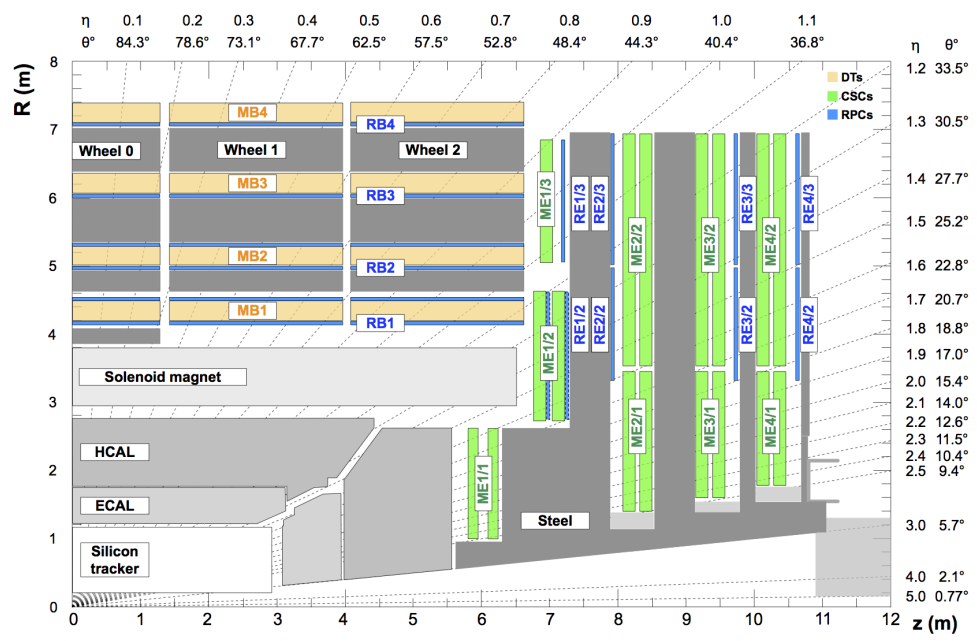
\includegraphics[width=0.9\textwidth]{fig/experiment/detector/muon_sys_r-z.png}
	\caption[Diagram of the CMS detector in the r-z plane showing the components of the muon system.]
	{Diagram of the CMS detector in the r-z plane showing the components of the muon system~\cite{CMS:2008xjf}.}
	\label{fig:muon_system}
\end{figure}

\section{Trigger System}
At the LHC, the proton beam crossing interval is 25 ns, which corresponds to a pp collision rate of 40 MHz. Recording the full set of detector information for each collision is unfeasible, as it 
would lead to far too much data to save to disk. As a result, the CMS experiment employs a two-tiered trigger system designed to preserve information of physics interest while reducing the 
stored event rate to a more manageable 100 Hz. The first level of the trigger (L1) is a hardware trigger, which reduces the event rate from 40 MHz to about 100 kHz. The second layer is the 
high level trigger (HLT), a processor farm using software optimized for fast processing. 

The L1 trigger is implemented using FPGAs and ASICs, and has local, regional, and global components. First, local patterns in the calorimeters, track segments, and hit patterns in the muon chambers 
are used by the Trigger Primitive Generators (TPGs). The TPGs rank and sort primitive objects corresponding to particle candidates based on energy, momentum, and reconstruction quality. Information
from the TPGs is taken as input by regional triggers for the calorimeters and muon systems. These regional triggers further determine candidate physics objects, as well as energy sums and isolation
information. Finally, this information is fed to a set of global triggers, which rank trigger objects across the entire detector. The final global trigger must decide whether to accept or 
reject an event based on information input from the global calorimeter and muon trigger systems. Algorithms used in this decision can be based on single object \pT thresholds and multiplicity-related 
thresholds, such as the presence of multiple jets, among other criteria. Events passing the L1 trigger are read out and passed to the HLT for further processing. 

In contrast to the L1 trigger, the HLT incorporates the full physics object reconstruction based on the full precision of the detector. This allows the HLT to accept and reject events with algorithms 
of similar quality to those used by offline analyses. Over 13,000 CPU cores are dedicated to HLT processing. For speed and efficiency, reconstruction and filtering algorithms are applied in increasing order of complexity. If a filter sequence fails, the rest of the reconstruction is skipped. Additionally, processing is done regionally based on the L1 candidates and relevant detector components 
passed as input to the HLT. Events that pass the HLT are assigned to relevant data streams based on their physics content. For this analysis, the relevant streams are the Double Muon and 
Double Electron streams, triggered by events with two muons or two electrons passing a set of minimum \pT requirements, among other cuts. 

\section{Object Reconstruction}
The global event reconstruction (also called particle-flow (PF) event reconstruction~\cite{CMS:2017yfk}) aims to reconstruct and identify each individual particle in an event, with an optimized combination of all subdetector information. In this process, the identification of the particle type (photon, electron, muon, charged hadron, neutral hadron) plays an important role in the determination of the particle direction and energy.

\begin{figure}
  \centering
   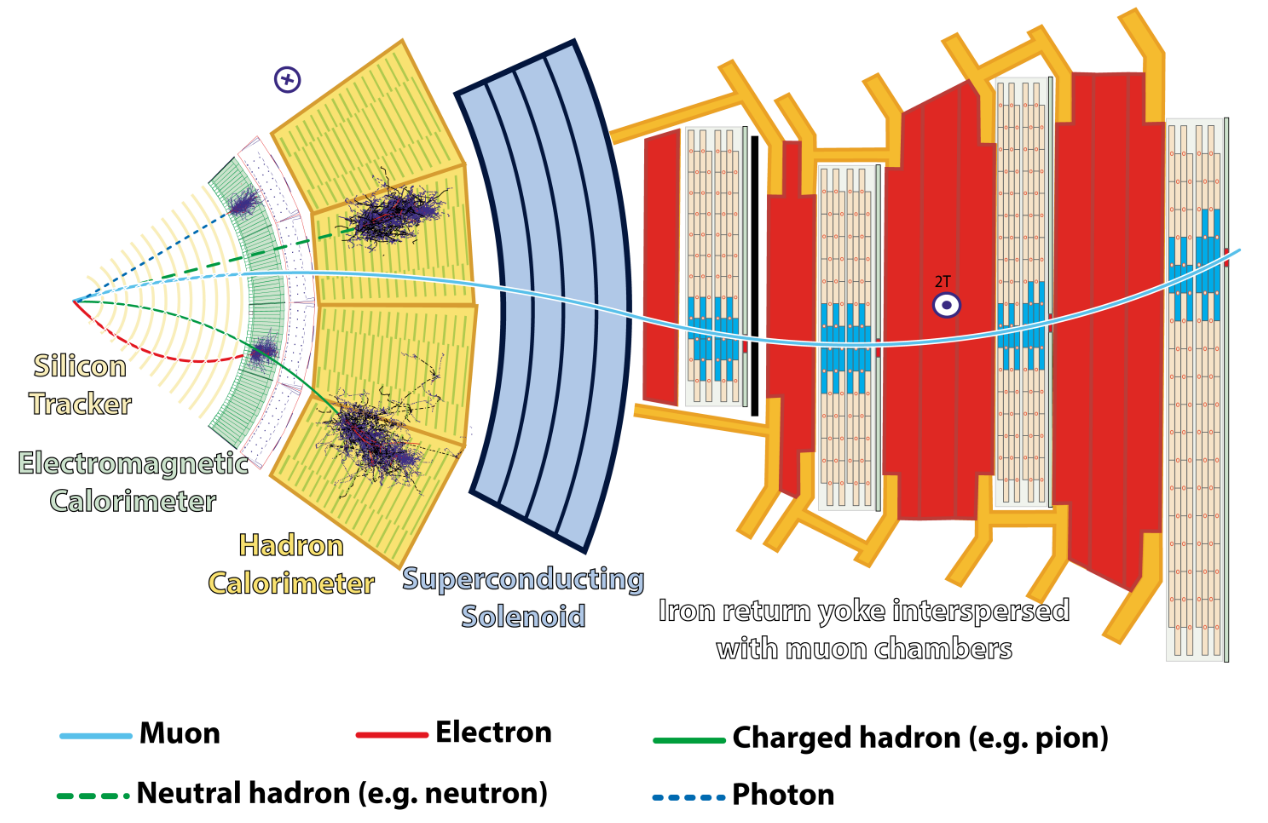
\includegraphics[width=0.9\textwidth]{fig/experiment/reconstruction/cms_detector.png}
	\caption{Schematic of different particles interacting with the CMS detector.}
\end{figure}

\subsection{Photon and Electron Reconstruction}
Photons and electrons interact with the material in the ECAL, depositing the majority of their energy before reaching the HCAL. As they interact, photons convert into 
electron-positron pairs and electrons radiate bremsstrahlung photons. This leads to the formation of an electromagnetic shower. Because of this, the original particle energy 
is split into multiple energy deposits, which must be combined to reconstruct the original energy. Deposits in individual ECAL crystals are combined into clusters, 
and these clusters are in turn combined into superclusters. Two algorithms are used to generate superclusters: the so-called "mustache" algorithm, and the so-called "refined" algorithm.
The mustache algorithm defines a seed cluster with energy above a certain threshold, and then combines it with other clusters within a region of the eta-phi plane centered at the 
seed location. The refined algorithm uses the mustache superclusters as well as tracking information to extrapolate bremsstrahlung and conversion tracks to decide whether a cluster should belong 
to the supercluster. 

The distinction between photons and electrons is made using tracking information, where photons are associated with no tracks and electrons with tracks. The Gaussian Sum Filter (GSF) [REF] track 
fitting algorithm is used to identify and characterize tracks that might be associated with an electron. It first begins with a hit pattern in the tracker, which is used as a seed. This seed 
can either be tracker-driven, coming from the collection of generic tracks tested for mutual compatibility, or it can be ECAL-driven, where a mustache supercluster is compared in location with 
a collection of tracker hit patterns to determine if the supercluster is consistent with the trajectory indicated by the track. Electron seeds are then converted into reconstructed electron tracks. 
In the absence of any GSF electron tracks, a photon candidate is obtained. Additional separation between photons and electrons is obtained through further selection requirements. 
The measured energy resolution for electrons produced in $\PZ$ boson decays in  $\Pp\Pp$ collision data ranges from $2$--$5$\%, depending on electron pseudorapidity and energy loss through bremsstrahlung in the detector material~\cite{CMS:2020uim}.

\subsection{Muon Reconstruction}
Muon reconstruction utilizes information from the muon detectors and the tracker. First, detector hits in the CSCs, DTs, and RPCs are used to build standalone tracks using a Kalman-filter technique.
Subsequently, these standalone muon tracks are combined with tracker information via two algorithms. So-called "tracker muons" are reconstructed using an "inside-out" algorithm, which starts from 
tracker tracks and matches them to DT or CSC segments. So-called "global muons" are reconstructed with an "outside-in" approach which starts from standalone muon tracks and matches them 
to tracker tracks using a Kalman-filter technique. In the case where both algorithms reconstruct a muon sharing the same tracker tack, the two outputs are merged into a single muon candidate.
In general, the tracker muon algorithm is more efficient in the region of low muon \pT, while the global algorithm is efficient at high \pT. 

The energy of muons is obtained from the corresponding track momentum. Matching muons to tracks measured in the silicon tracker results in a \pt resolution, for muons with \pt up to $100$\GeV, of $1$\% in the barrel and $3$\% in the endcaps. The \pt resolution in the barrel is better than $7$\% for muons with \pt up to $1$\TeV~\cite{CMS:2018rym}.


\subsection{Hadrons}
Charged hadrons are identified as charged particle tracks that are neither identified as electrons nor as muons. Neutral hadrons are identified as HCAL energy clusters not linked to any charged hadron trajectory, or as a combined ECAL and HCAL energy excess with respect to the expected charged hadron energy deposit.

\subsection{Jets}
For each event, hadronic jets are reconstructed as clusters of PF particles, including photons, electrons, muons, and hadrons. For clustering, the infrared and collinear-safe anti-\kt algorithm~\cite{Cacciari:2008gp, Cacciari:2011ma} is used. The goal of jet clustering algorithms is to combine PF particles together into a single jet object by merging them together based on their relative geometric distances and transverse momenta (\kt). In the case of the anti-\kt algorithm, clustering proceeds from smallest geometric distance to largest, weighted by squared inverse \kt. This inverse weighting 
preferentially combines PF particles with higher momenta before lower momenta, for a given distance. The advantage of this approach is that low momentum particles are more likely to be clustered 
with high momentum counterparts, rather than with other low momentum particles. It follows that these low momentum particles will not significantly modify the jet shape, whereas the more important, high-momentum particles, will. A precise definition of the anti-\kt algorithm is defined in equation \ref{eq:antikt}. 

\begin{equation}
	d_{ij} = min(k_{T,i}^{2p}, k_{T,j}^{2p})\frac{(\eta_i - \eta_j)^2 + (\phi_i - \phi_j)^2}{R^2},\;\; d_i = k_{T,i}^{2p}
	\label{eq:antikt}
\end{equation}

In equation \ref{eq:antikt}, the indices i and j refer to two PF particles, the parameter $p$ is taken to be -1, and the radius parameter $R$ is parameter that can be tuned. For standard jets in CMS, as used in this analysis, $R$ is set to 0.4. Particles are clustered from smallest $d_{ij}$ to largest until there is no $d_{ij}$ smaller than $k_{ti}^{-2}$, at which point the final jet is defined. A visual representation of the anti-\kt algorithm is shown in Fig. \ref{fig:anti_kt_diagram}.

\begin{figure}
  \centering
   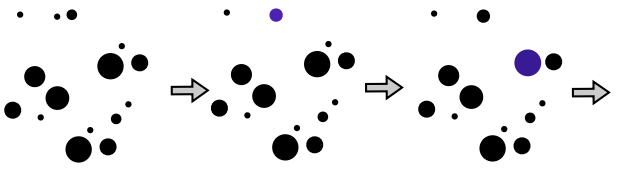
\includegraphics[width=0.9\textwidth]{fig/experiment/reconstruction/jet_clustering.png}
	\caption{An example of the first few steps of the anti-\kt jet clustering algorithm.}
	\label{fig:anti_kt_diagram}
\end{figure}

Jet momentum is determined as the vectorial sum of all particle momenta in the jet, and is found from simulation to be, on average, within $5$--$10$\% of the true momentum over the entire \pt spectrum and detector acceptance. Additional $\Pp\Pp$ interactions within the same or nearby bunch crossings (pileup) can contribute additional tracks and calorimetric energy depositions to the jet momentum. To mitigate this effect, charged particles identified to be originating from pileup vertices are discarded and an offset correction is applied to correct for remaining contributions~\cite{CMS:2020ebo}. The jet energy resolution typically amounts to $15$--$20$\% at $30$\GeV, $10$\% at $100$\GeV, and $5$\% at $1$\TeV~\cite{CMS:2016lmd}.

\begin{figure}
  \centering
   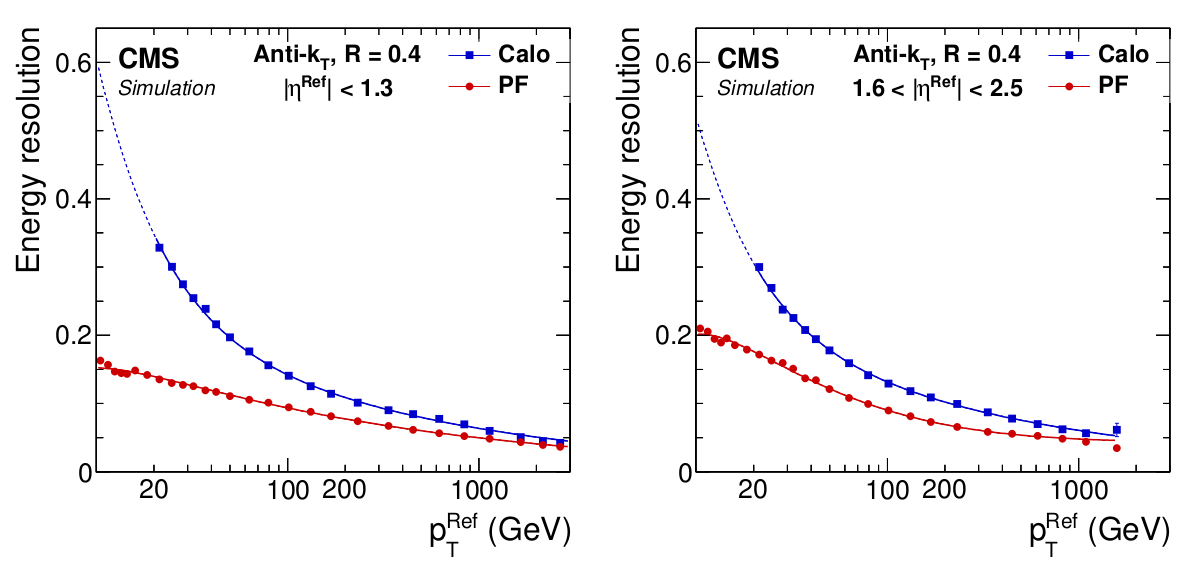
\includegraphics[width=0.9\textwidth]{fig/experiment/reconstruction/jet_energy_resolution.png}
	\caption{Jet energy resolution as a function of simulated jet \pT in the barrel (left) and in the endcap (right) regions. Calo refers to the sum of ECAL and HCAL energy deposits, 
	while PF corresponds to jets clustered from PF particles using the anti-\kt algorithm.}
	\label{fig:anti_kt_diagram}
\end{figure}



\chapter{Overview of Analysis Strategy}

Before discussing the full details of the analysis procedure and results, it is worth summarizing 
the broader strategy taken in our search for \hzg. As two prior CMS results have 
been published with Run 1 data and 2016 data, we will emphasize the ways in which our analysis
overlaps and differs from these previous approaches. Very broadly, the current search is 
similar to the previous analyses in trigger, object, and basic event selection. 
However, it is significantly more advanced in three body mass reconstruction, 
event categorization, and background modeling. We will show that the innovations in these 
areas have significantly improved the expected sensitivity and statistical robustness of the search 
with respect to the past CMS analyses.

Chapter 5 provides a detailed description of the data and Monte Carlo simulation 
used in our analysis. Standard dimuon and dielectron trigger streams are used for 2016, 2017, 
and 2018 LHC data. The full dataset corresponds to an integrated luminosity of 
137 $fb^{-1}$. In other words, we use the full CMS Run 2 dataset at 13 TeV center of 
mass energy. Simulated signal samples are used to determine the expected signal yields 
and three body mass shape. Simulated background samples are used for MVA training 
and category optimization. However, the background shape and normalization in the final result
is determined by fitting the data and does not rely on any simulation.

Chapter 6 describes the basic object and event selection used in the analysis, and Chapter 7 
describes further selection and categorization using MVAs. As mentioned, the basic 
selection requirements are fairly similar to previous CMS analyses. Muons are selected with 
a loose cut-based ID, while electrons and photons are selected with loose MVA IDs. Loose ID
requirements are chosen in order to maximize signal efficiency. Background is then suppressed 
through a combination of basic cuts and MVA methods. Basic kinematic cuts on isolation, mass, 
and photon energy variables are able to significantly reduce backgrounds from initial and final 
state radiation, while the MVA methods are able to strongly disciminate against backgrounds from 
jets misreconstructed as photons. Finally, a kinematic fit procedure in the dilepton mass 
is able to significantly improve the signal mass resolution. The kinematic fit is an 
innovation of the current analysis and contributes to its improved sensitivity.

Chapter 8 details the approach to signal and background modeling of the three body 
mass spectrum. As in previous CMS \hzg searches, the 
signal shape is determined via an analytic fit to simulation. A resonant background 
contribution from \hmumu is modeled similarly. The nonresonant 
background contribution is taken from a fit to data in the range of 105 to 170 GeV. This 
background model includes both the turn-on arising from the real Z boson peak as well as 
the falling spectrum at higher mass. We note that the turn-on was fit in the Run 1 analysis as 
well, but was dropped in the 2016 analysis. A more thorough discussion of the merits of fitting 
the turn-on will be described in chapter 8.

Chapter 9 describes the systematic uncertainties relevant for the analysis, and Chapter 10
gives a basic overview of the statistics used to arrive at the final results. It is 
worth noting that given the current integrated luminosity, the analysis is dominated by 
statistical uncertainty. Chapter 11 gives the full set of results, including best fit 
signal strength, limits, and comparisons with \hgg. 




\chapter{Data and Simulated Samples}\label{sec:data}

The data sample used for the CMS Run 2 \hzg{} search corresponds to a total integrated luminosity of \LumiT\fbinv and was collected over a data-taking period spanning three years: \Lumia\fbinv in 2016, \Lumib\fbinv in 2017, and \Lumic\fbinv in 2018~\cite{CMS-LUM-17-003,LUM-17-004,LUM-18-002}. 
To be considered in the analysis, events must satisfy the HLT requirements for at least one of the dielectron or dimuon triggers.
The dielectron trigger requires a leading (subleading) electron with
$\pt > 23\,(12)\GeV$, while the dimuon trigger requires a leading (subleading) muon with $\pt > 17\,(8)\GeV$.
The corresponding CMS data streams are listed in Table \ref{tab:data_samples}. All data samples use the CMS MINIAOD data format.
To ensure data quality, luminosity masks are applied based on recommendations from the Physics Performance and Dataset group.

\begin{table}[tb]
  \begin{center}
	  \caption{Summary of MINIAOD data samples used.}
    \begin{tabular}{|l|l|}
      \hline
	    \textbf{$\Pe^+\Pe^-\PGg$ final state} & \textbf{$\PGm^+\PGm^+\PGg$ final state}	                     \\\hline 
      /DoubleEG/Run2016B-17Jul2018\_ver2-v1 	&  /DoubleMuon/Run2016B-17Jul2018\_ver2-v1   \\
      /DoubleEG/Run2016C-17Jul2018-v1 		&  /DoubleMuon/Run2016C-17Jul2018-v1         \\
      /DoubleEG/Run2016D-17Jul2018-v1 		&  /DoubleMuon/Run2016D-17Jul2018-v1         \\
      /DoubleEG/Run2016E-17Jul2018-v1	        &  /DoubleMuon/Run2016E-17Jul2018-v1         \\       
      /DoubleEG/Run2016F-17Jul2018-v1	        &  /DoubleMuon/Run2016F-17Jul2018-v1         \\       
      /DoubleEG/Run2016G-17Jul2018-v1	        &  /DoubleMuon/Run2016G-17Jul2018-v1         \\
      /DoubleEG/Run2016H-17Jul2018-v1	        &  /DoubleMuon/Run2016H-17Jul2018-v1         \\
      /DoubleEG/Run2016H-17Jul2018-v1	        &  /DoubleMuon/Run2016H-17Jul2018-v1         \\
      /DoubleEG/Run2017B-31Mar2018-v1	        &  /DoubleMuon/Run2017B-31Mar2018-v1         \\
      /DoubleEG/Run2017C-31Mar2018-v1	        &  /DoubleMuon/Run2017C-31Mar2018-v1         \\
      /DoubleEG/Run2017D-31Mar2018-v1	        &  /DoubleMuon/Run2017D-31Mar2018-v1         \\
      /DoubleEG/Run2017E-31Mar2018-v1	        &  /DoubleMuon/Run2017E-31Mar2018-v1         \\       
      /DoubleEG/Run2017F-31Mar2018-v1	        &  /DoubleMuon/Run2017F-31Mar2018-v1         \\           
      /EGamma/Run2018A-17Sep2018-v2		&  /DoubleMuon/Run2018A-17Sep2018-v2         \\  
      /EGamma/Run2018B-17Sep2018-v1		&  /DoubleMuon/Run2018B-17Sep2018-v1         \\
      /EGamma/Run2018C-17Sep2018-v1		&  /DoubleMuon/Run2018C-17Sep2018-v1         \\
      /EGamma/Run2018D-22Jan2019-v2		&  /DoubleMuon/Run2018D-PromptReco-v2        \\\hline       
    \end{tabular}
    \label{tab:data_samples}
  \end{center}
\end{table}

Signal samples for $\Pg\Pg\PH$, VBF, $\mathrm{V}\PH$, and $\ttbar\PH$ production, with 
$\PH\to\PZ\gamma$ and $\PZ\to\ell^+\ell^-$ ($\ell = \Pe$, $\mu$, or $\tau$),
are generated at next-to-leading order (NLO) using \POWHEG v2.0~\cite{cite:powheg1,cite:powheg2}.
These samples are produced for $m_\PH$ of $120$, $125$, and $130$\GeV. 
The dominant backgrounds, $\PZ/\gamma^{*}(\rightarrow \ell^+\ell^-)$+$\gamma$ and $\PZ/\gamma^{*}(\rightarrow \ell^+\ell^-)$+jets,
are generated at NLO using the \MGvATNLO v2.6.0 (v2.6.1) 
generator~\cite{Alwall:2014hca} for 2016 (2017 and 2018) samples. 
 Events arising from $\ttbar$ production~\cite{Frixione:2007nw} are a relatively minor background and are generated at NLO with \POWHEG v2.0~\cite{cite:powheg1,cite:powheg2}.
 The background from vector boson scattering (VBS) production of $\PZ/\gamma^{*}$+$\gamma$ pairs, with the $\PZ$ boson decaying to a pair of leptons, is simulated at leading order using the \MGvATNLO generator. The decay $\PH\to\mu^+\mu^-$ is considered as a resonant background and is generated for the $\Pg\Pg\PH$, VBF,  $\mathrm{V}\PH$, and $\ttbar\PH$ production mechanisms. The $\Pg\Pg\PH$ production cross section is
computed at next-to-next-to-NLO precision in QCD and at NLO in electroweak (EWK)
theory~\cite{Anastasiou:2016cez}. 
The cross sections for Higgs boson production in the VBF~\cite{PhysRevLett.115.082002} and VH~\cite{BREIN2004149} mechanisms are calculated at next-to-NLO in QCD, including NLO EWK corrections, while the $\ttbar\PH$ cross section is computed at NLO in QCD and EWK theory~\cite{PhysRevD.68.034022}. 

A full list of simulated physics processes used in the analysis is provided in Table \ref{tab:sim_samples}, along with cross section and branching fraction information. 
For the \hzg{} and $\PH\to\mu^+\mu^-$ samples, the SM Higgs boson production cross sections and branching fractions
recommended by the LHC Higgs Working
Group~\cite{LHC-YR4} are used for each mass point.
The values for the Higgs boson processes listed in Table \ref{tab:sim_samples} correspond to $m_{\PH}=125\GeV$.

\begin{table}[tb]
	\begin{center}
		\caption{Simulated event samples used in the analysis. For Higgs samples, the listed cross sections and branching fractions correspond to the values for $m_{\PH}=125\GeV$.}
		\begin{tabular}{|l|c|c|}
			\hline
			\textbf{process} & \textbf{cross section (pb)} & \textbf{branching fraction}\\\hline 
			$\mathrm{gg}\PH\to\PZ\gamma\to\lplm\gamma$ & 48.58 & $1.548\times 10^{-3}$ \\ 
			$\mathrm{q\bar{q}}\PH\to\PZ\gamma\to\lplm\gamma$ & 3.782 & $1.548\times 10^{-3}$\\
			$\PZ\PH\to\PZ\gamma\to\lplm\gamma$ & 0.8839 & $1.548\times 10^{-3}$\\ 
			$\PW^+\PH\to\PZ\gamma\to\lplm\gamma$ & 0.84 & $1.548\times 10^{-3}$\\
			$\PW^-\PH\to\PZ\gamma\to\lplm\gamma$ & 0.532 & $1.548\times 10^{-3}$\\ 
			$\ttbar\PH\to\PZ\gamma\to\lplm\gamma$ & 0.5071 & $1.548\times 10^{-3}$\\ 
			$\mathrm{gg}\PH\to\mpmm$ & 48.58 & $2.176\times 10^{-4}$\\ 
			$\mathrm{q\bar{q}}\PH\to\mpmm$ & 3.782 & $2.176\times 10^{-4}$\\
			$\PZ\PH\to\mpmm$ & 0.8839 & $2.176\times 10^{-4}$\\ 
			$\PW^+\PH\to\mpmm$ & 0.84 & $2.176\times 10^{-4}$\\
			$\PW^-\PH\to\mpmm$ & 0.532 & $2.176\times 10^{-4}$\\ 
			$\ttbar\PH\to\mpmm$ & 0.5071 & $2.176\times 10^{-4}$\\ 
			$\PZ/\gamma^*\to\lplm\gamma$ & 117.864 & --\\
			$\PZ/\gamma^*\to\lplm$+jets & 6225.42 & --\\
			$\ttbar$ (inclusive) & 831.76 & --\\
			VBF $\PZ/\gamma^*+\gamma$ & 0.1097 & --\\

			\hline
		\end{tabular}
		\label{tab:sim_samples}
	\end{center}
\end{table}

All simulated events are interfaced
with \PYTHIA v8.226~(v8.230)~\cite{Sjostrand:2014zea} with the
CUETP8M1~\cite{Khachatryan:2015pea} (CP5~\cite{Sirunyan:2019dfx}) underlying event tune for 2016 (2017--2018) for the
fragmentation and hadronization of partons and the internal bremsstrahlung of the leptons. The NLO parton distribution function (PDF) set, NNPDF v3.0~\cite{nnpdf30}~(NNPDF v3.1)~\cite{nnpdf_new}, is used to produce these samples in 2016 (2017--2018). The response of the CMS detector is modeled using the
\GEANTfour  program~\cite{AGOSTINELLI2003250}. 
The simulated events are reweighted to correct for differences between data and simulation in the number of additional $\Pp\Pp$ interactions, trigger efficiencies, selection efficiencies, and efficiencies of isolation requirements for photons, electrons, and muons. These corrections and their associated uncertainties will be described in more detail throughout the remainder of this thesis. The rest of this chapter will discuss general procedures and corrections related to the data and simulated samples.

\section{Z+jets Overlap Removal}
The two dominant backgrounds in this analysis are $\PZ/\gamma^{*}(\rightarrow \ell^+\ell^-)$+$\gamma$, or $\PZ\gamma$ for short, and $\PZ/\gamma^{*}(\rightarrow \ell^+\ell^-)$+jets, or $\PZ$+jets for short. Both processes 
are simulated independently in order to obtain the best model of the kinematics of the $\lplm\gamma$ system. 
The $\PZ\gamma$ sample simulates photons from initial-state and final-state radiation at the matrix element level and includes a better 
computation of the interference between the corresponding Feynman diagrams than the $\PZ$+jets sample.
However, the $\PZ$+jets
simulated sample also includes the contribution from $\PZ\gamma$. Therefore, this contribution must be removed from the 
$\PZ$+jets sample in order to avoid double counting events and to utilize the better kinematic modeling of the $\PZ\gamma$
sample. To handle this, $\PZ$+jets events are removed from the analysis if they contain prompt, final state photons within 
$\DR = \sqrt{\smash[b]{(\Delta\phi)^2 + (\Delta\eta)^2}} = 0.1$ of the photon selected to reconstruct the $\lplm\gamma$ system.
The events with prompt, final state photons are tagged using generator-level truth information.

\section{Photon Internal Conversion}
\label{sec:gconversion}
It was noticed by the $\PH\to\PGg\PGg$ group that Pythia 8 showering automatically 
includes a component in which $\PH\to\PGg\PGg$ photons are 
``internally converted'' into  $\PH\to\PGg\PGg*\to ff\PGg\PGg$ 
(with $ff$ mostly $ee$). This also affects the $\PH\to \PZ\PGg$ and SM $\PZ\PGg$ samples. 
We lose some events with $\PGg^{*}$ decay to fermions since they do not pass our selection of 
2 leptons plus a photon. 
Since the normalization of the samples
does not include the internal conversion component, the cross section has to be adjusted accordingly.
To determine the number by which the cross section is adjusted, we measure the internal conversion
rate in MC. 
We define a ratio where the numerator is the number of photons flagged as
\textbf{fromHardProcessFinalState} 
and the denominator is total number of events in the MC. Subtracting this ratio from 1 gives
the internal conversion rate.
In our analysis, the internal conversion rate is ~3.1\%(2016) and ~3.0\%(2017).  
We therefore divide our cross sections by 0.969 (0.97) for 2016 (2017 and 2018).

\section{Transverse Momentum Reweighting}\label{sec:Zpt}
For the 2016 MC, the underlying event tuning was developed in Run-1 with 7 \TeV data. 
To get a more appropriate underlying description, the GEN group provided a new tuning
for 2017 and 2018 MC production, updating from CUETP8M1 (2016) to CP5 (2017/2018).
However, a discrepency was found in the $\ell\ell\gamma$ \pt spectrum
which had an obvious and significant impact in the SM $Z\gamma$ sample. 
Since $\pt^{ll\gamma}/m_{ll\gamma}$ is an important variable in the kinematic MVA training, 
we correct for this issue by reweighting the $\pt^{ll\gamma}$ from simulation to data in 
2017 and 2018 using a sideband region. 
We define the sideband region as $115GeV<m_{ll\gamma}<120GeV$ and $130GeV<m_{ll\gamma}<135GeV$,
which is chosen close to signal region to avoid differences in kinematics.
We evaluate this weight for the electron and muon channels for 2017 and 2018.
\begin{figure*}[htbp]
	\begin{center}
		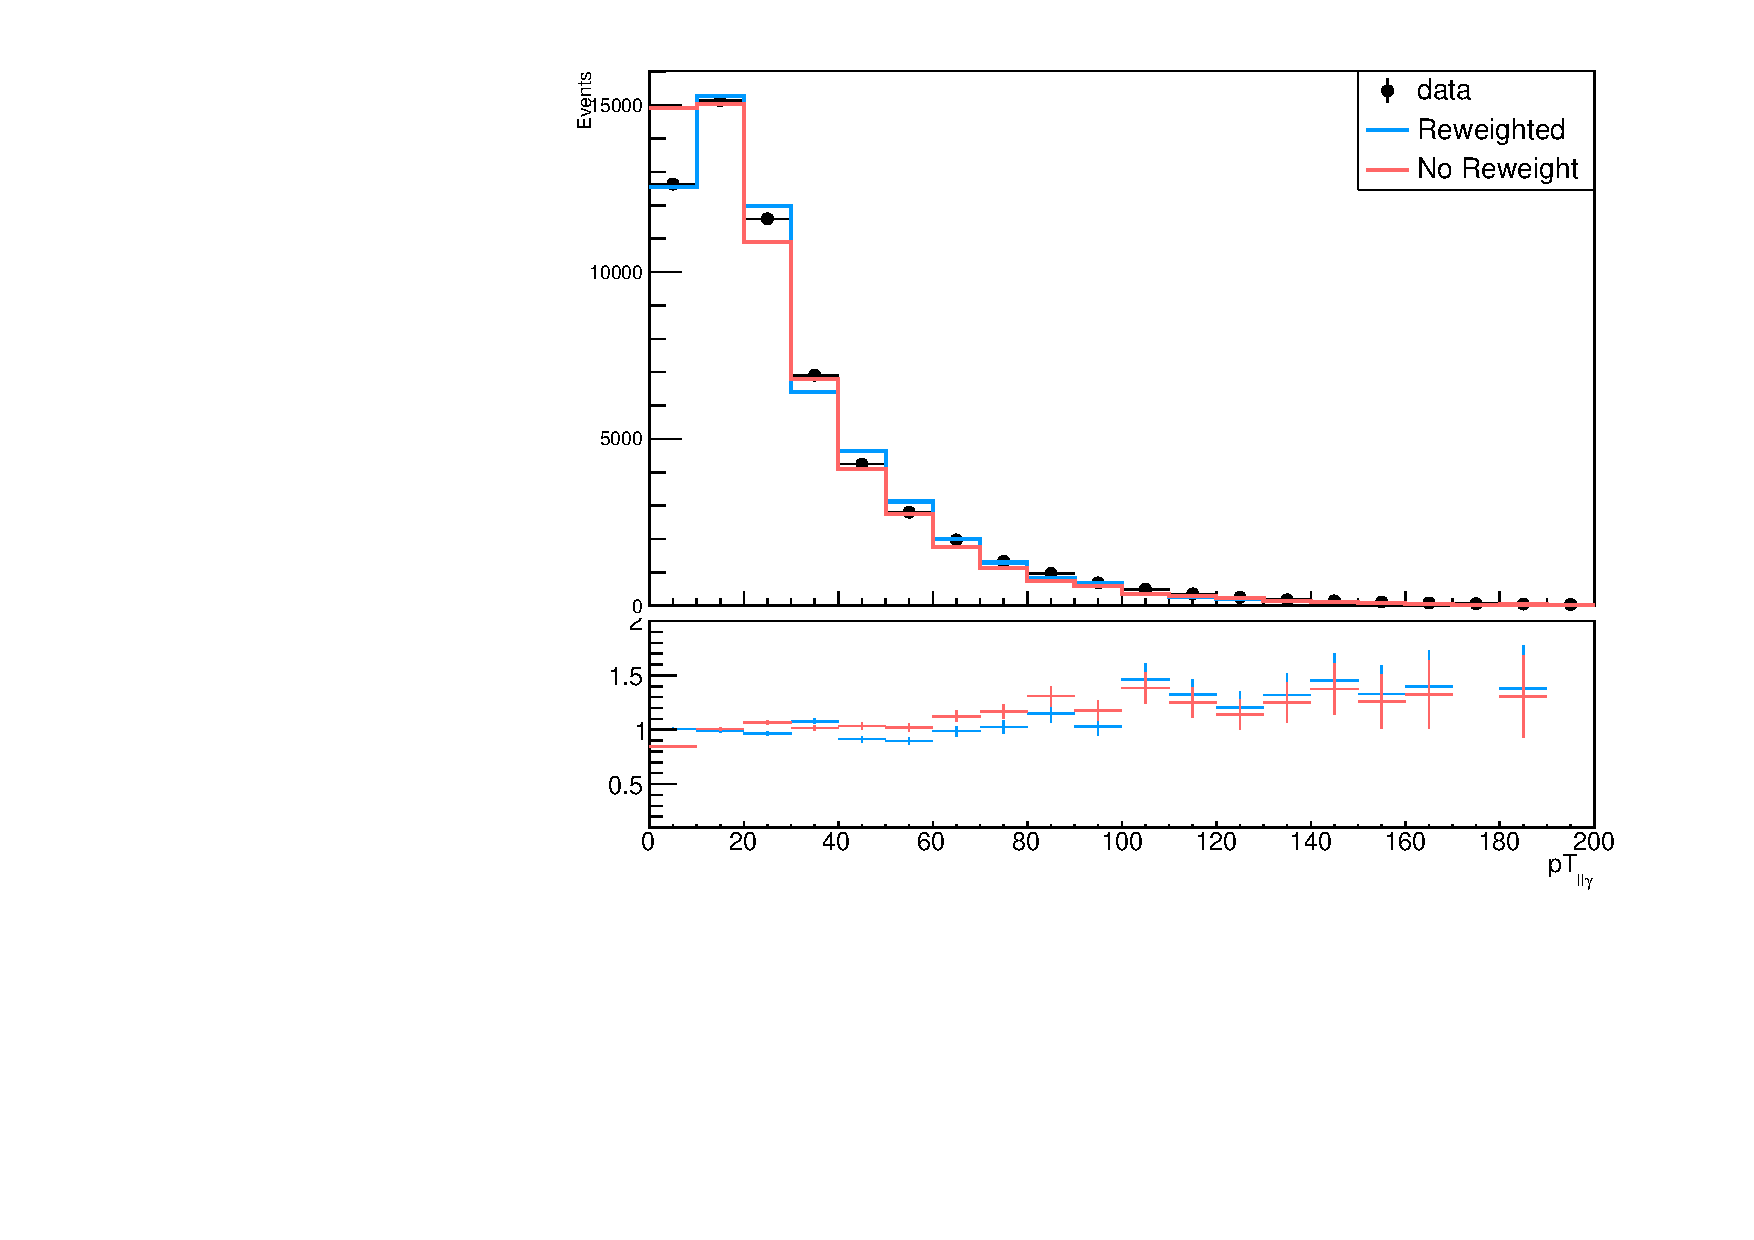
\includegraphics[width=0.35\textwidth]{fig/zpt_reweight/zgptrewei_datasb17.pdf}
		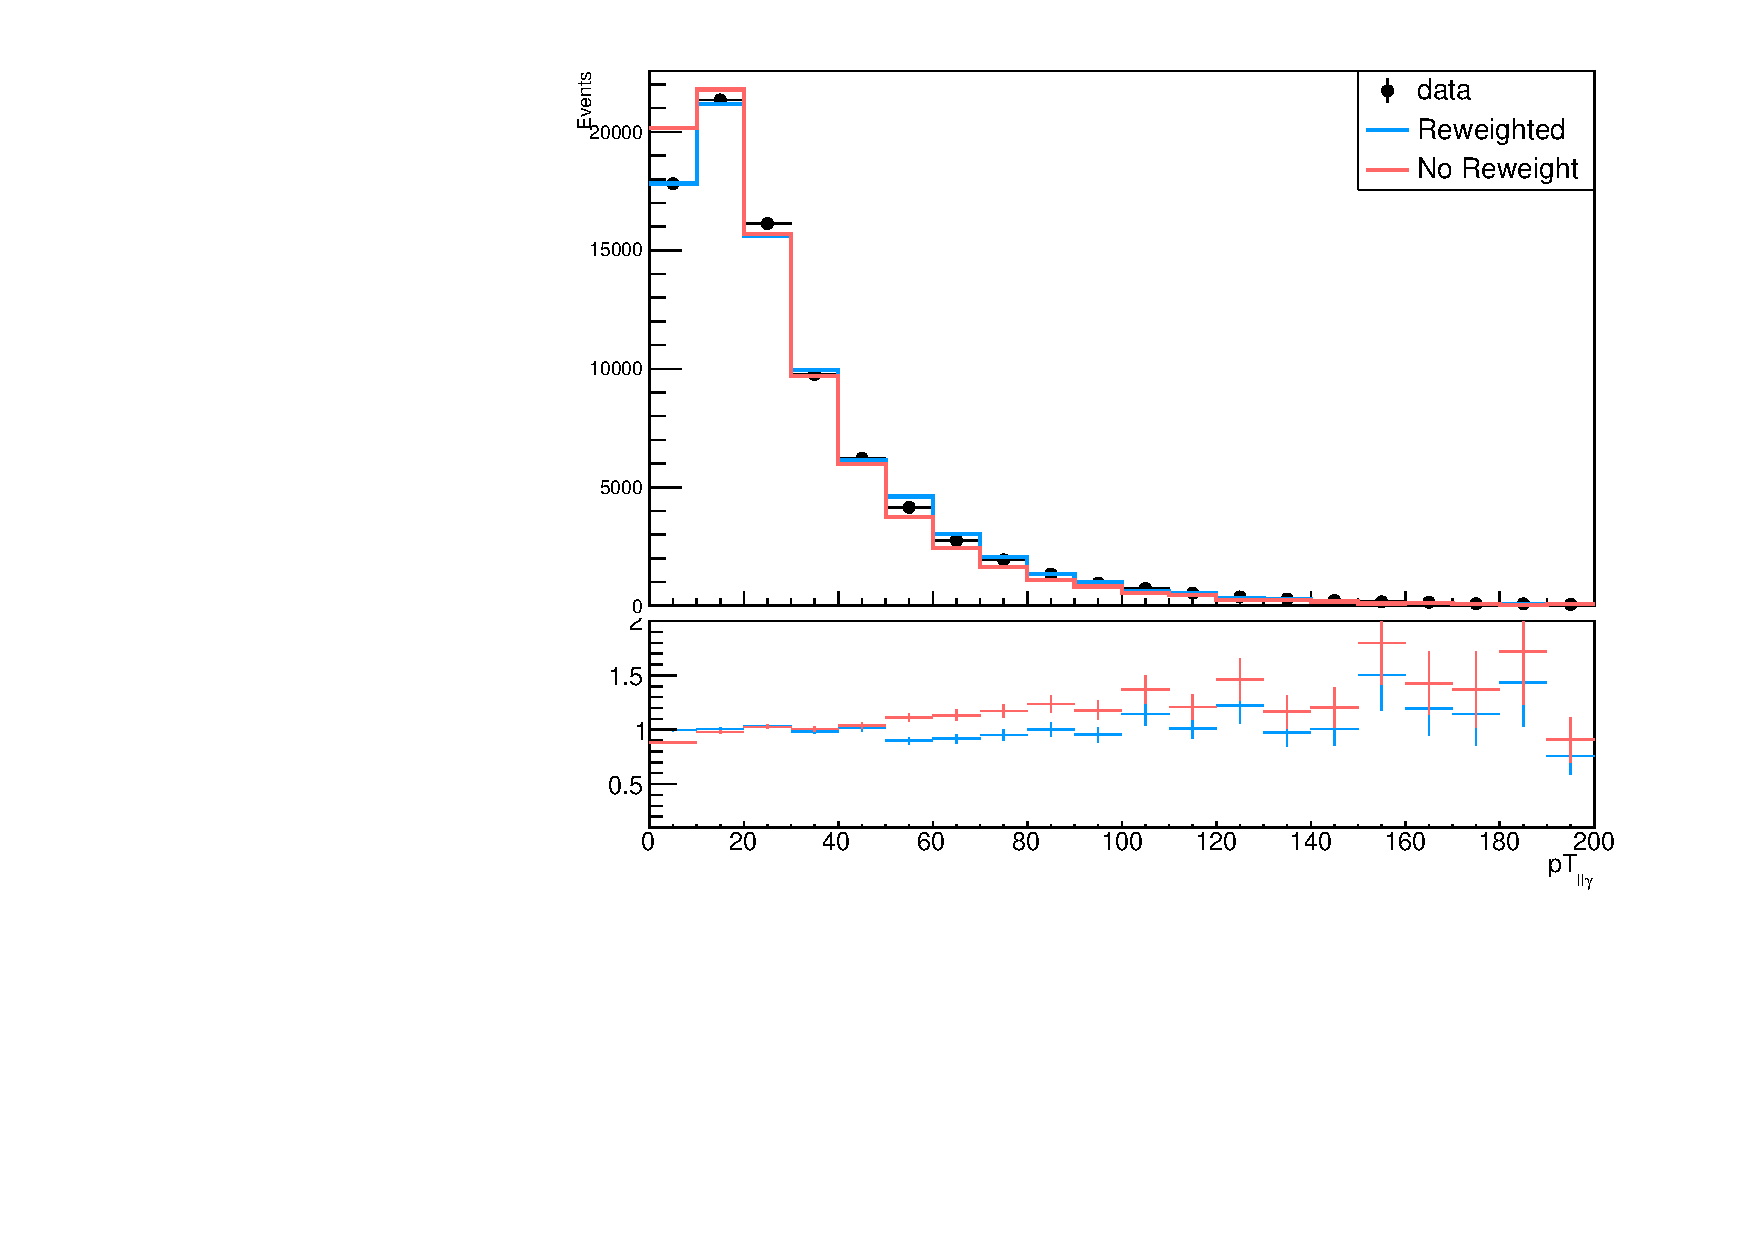
\includegraphics[width=0.35\textwidth]{fig/zpt_reweight/zgptrewei_datasb18.pdf}
	\end{center}
	\caption{Simulation before and after the correction to the $\ell\ell\gamma$ \pt.
    The black points show the data. Left:2017, right: 2018.}
\end{figure*}

\section{Pileup Reweighting}\label{sec:pileup}
The simulation includes an accurate distribution of the number of interactions 
taking place in each bunch crossing. Although the Deterministic Annealing primary vertex reconstruction \cite{detanneal} has been shown to
be efficient and well-behaved up to the observed levels of pileup, the final distribution
for the number of reconstructed primary vertices is still sensitive to differences between data and 
MC in the primary vertex reconstruction and underlying event.
Additionally, there is a potentially larger effect where the distribution for the number of
reconstructed vertices can be biased by the offline event selection criteria and even by the trigger.
In order to factorize these effects, instead of reweighting the MC by the number of 
reconstructed Primary Vertices, we reweight the number of pileup interactions in the simulation 
(as stored in the PileupInfo collection in the MC). The pileup distribution for data is
derived by using the per-bunch-crossing-per-luminosity-section instantaneous luminosity from
the LumiDB together with the total pp inelastic cross section. The total pp inelastic cross 
section is taken to be 66 mb, 72.4 mb, and 80 mb for 2016, 2017, and 2018 respectively.
This yields an expected pileup distribution, correctly weighted by the 
per-bunch-crossing-per-luminosity-section integrated luminosity over the entire data-taking period. The inelatistic cross-sections are choosing the  
Figure \ref{fig:puwei} shows the number of primary vertices distribution after 
pile-up reweighting in
the $ee\PGg$ channel. 
\begin{figure}[hbtp]
  \begin{center}
     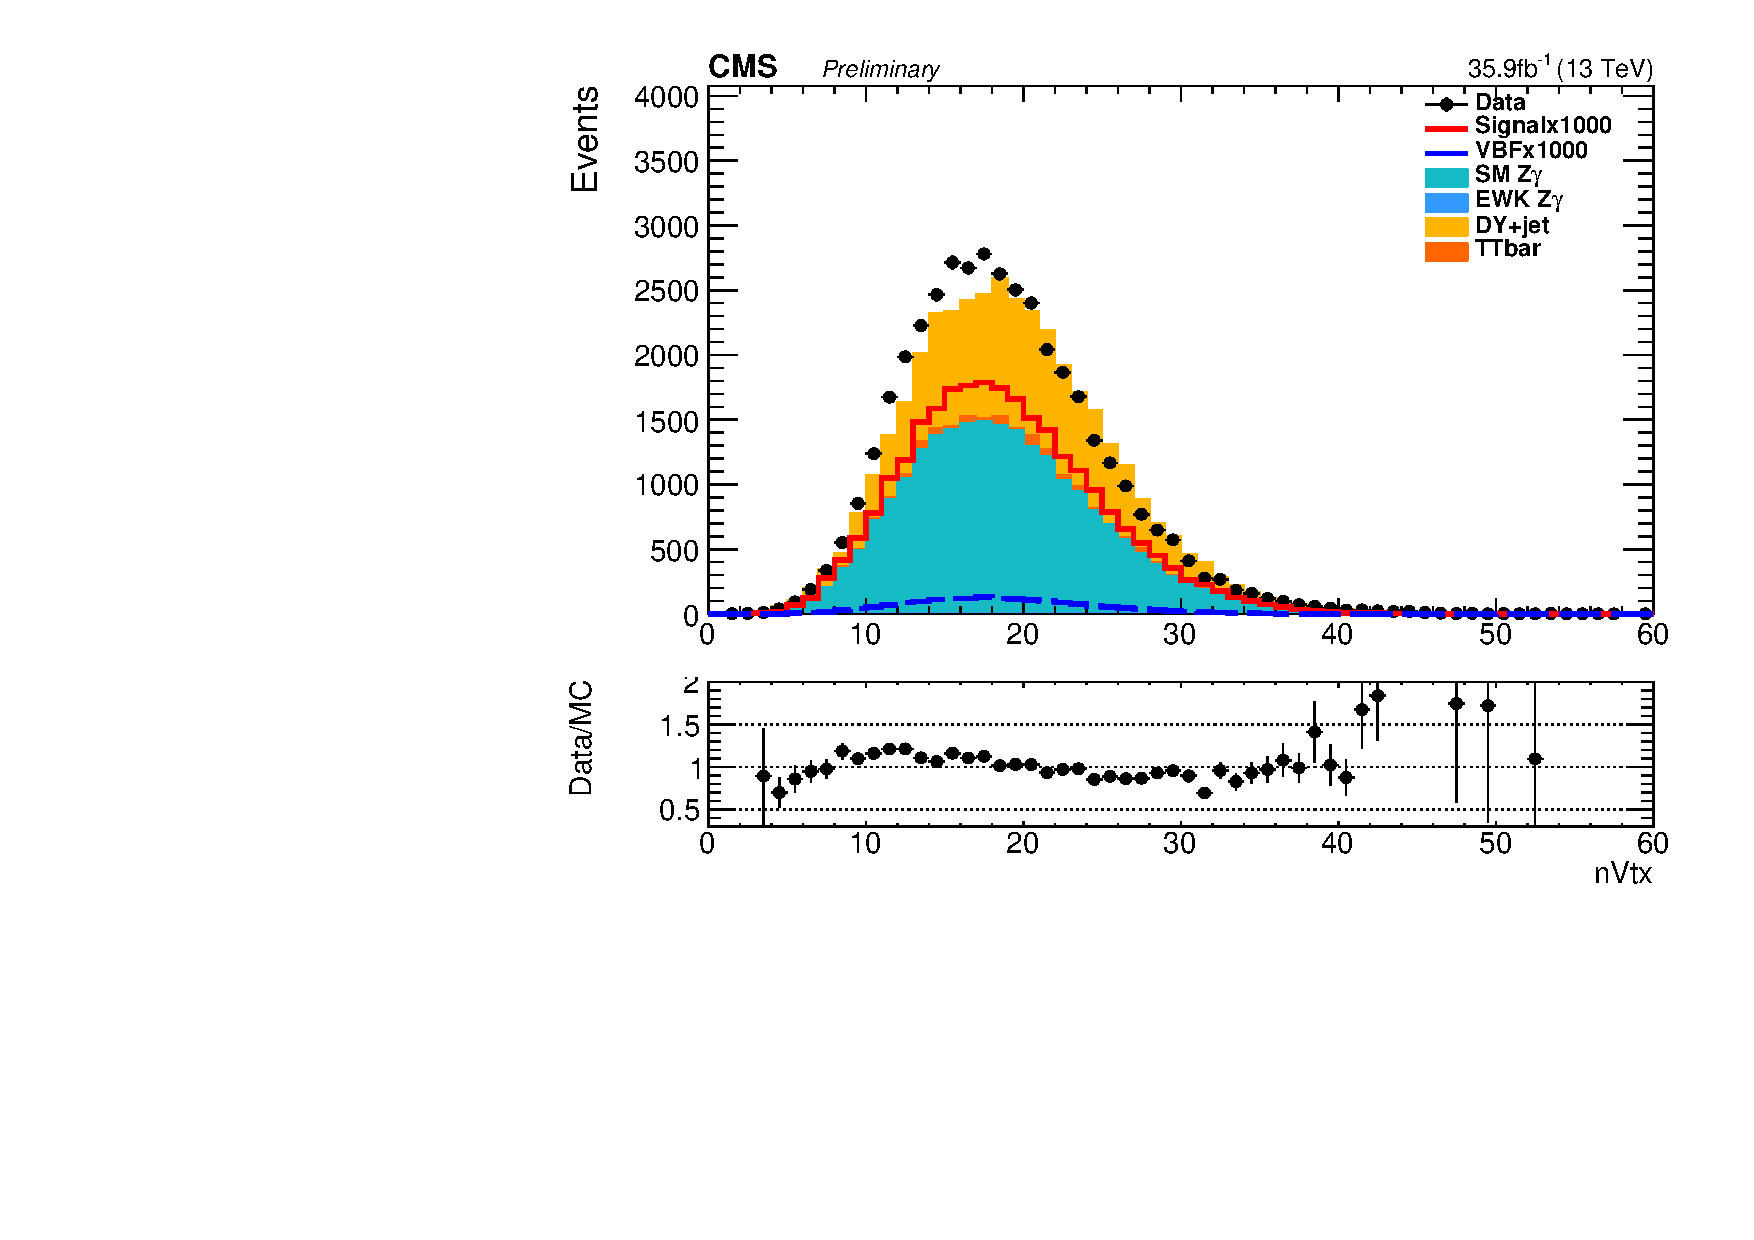
\includegraphics[width=0.3\textwidth]{fig/pileup/ele_kin_nVtx_valid_Legacy16_HLT.pdf}
     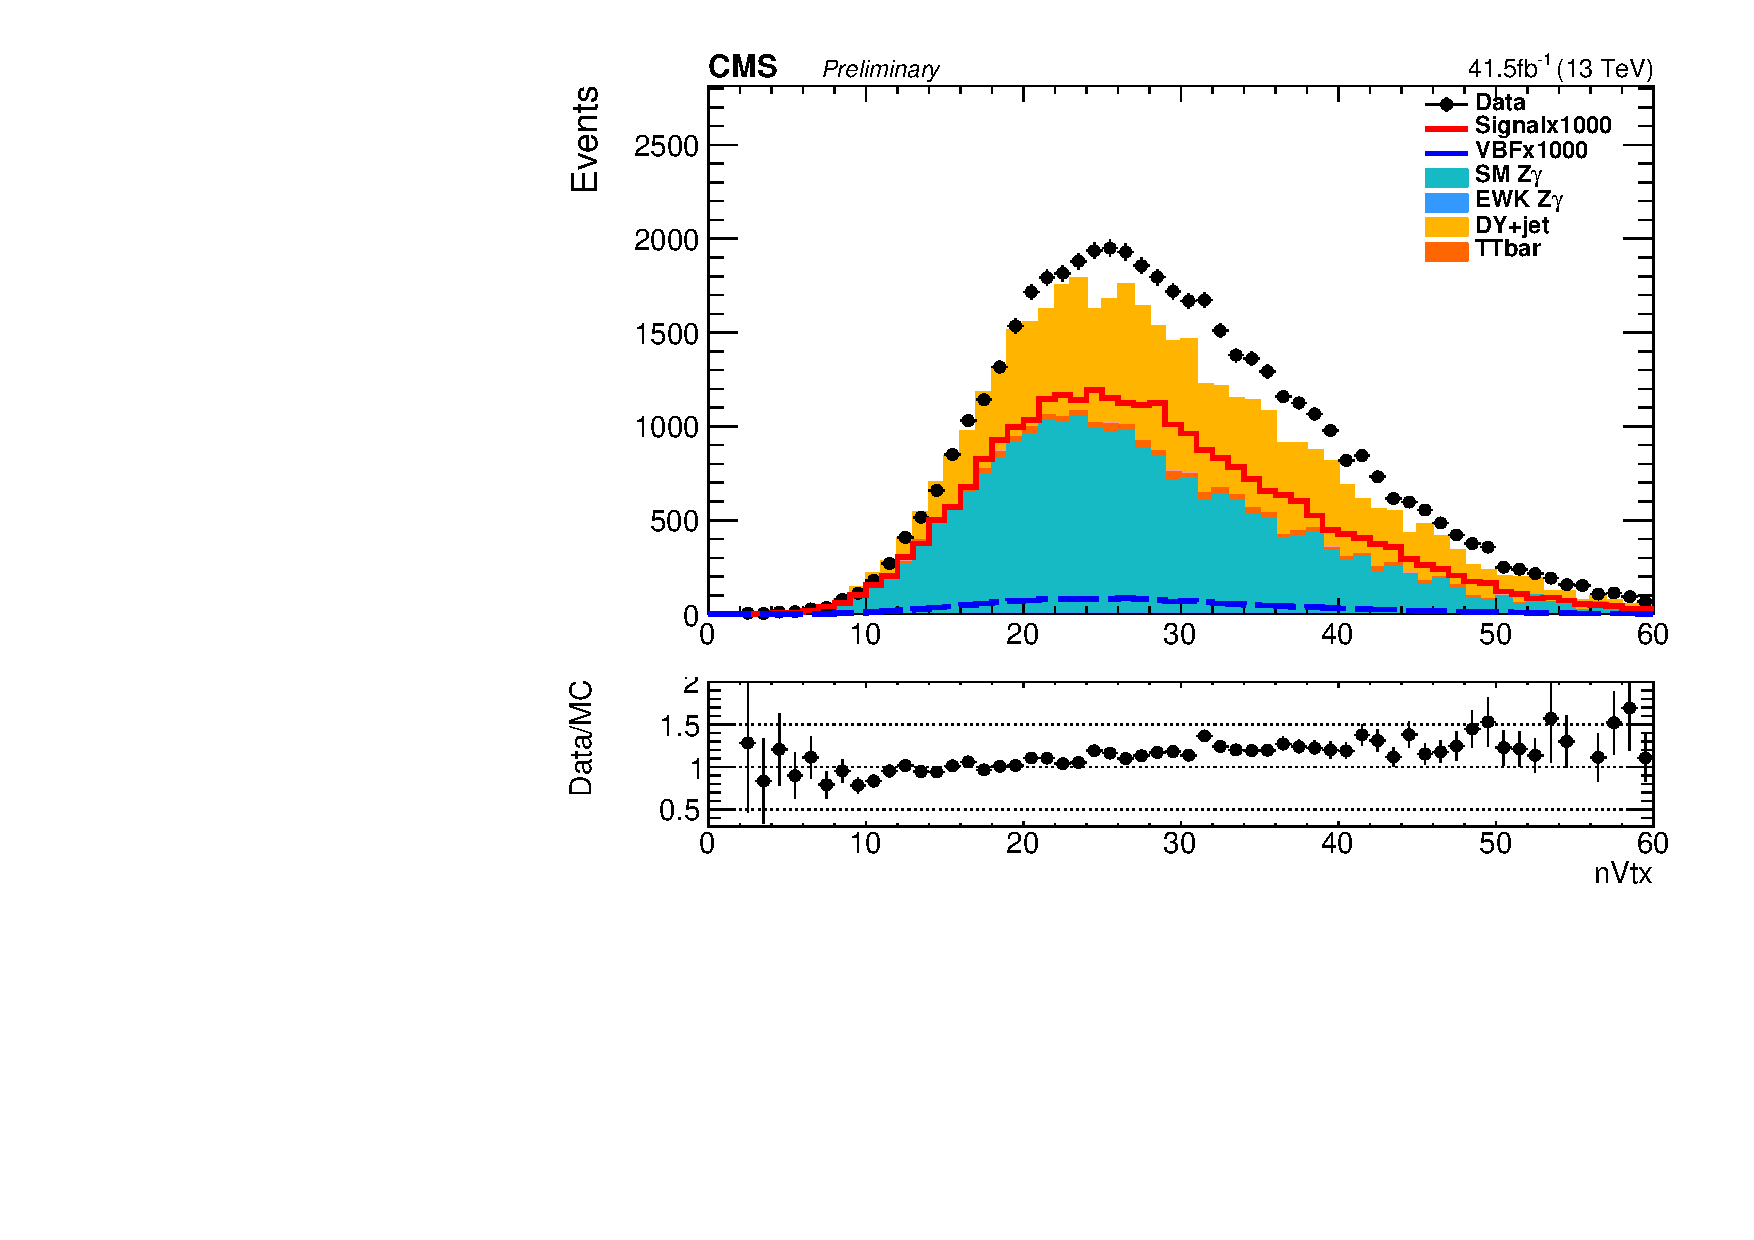
\includegraphics[width=0.3\textwidth]{fig/pileup/ele_kin_nVtx_valid_Rereco17_HLT.pdf}
     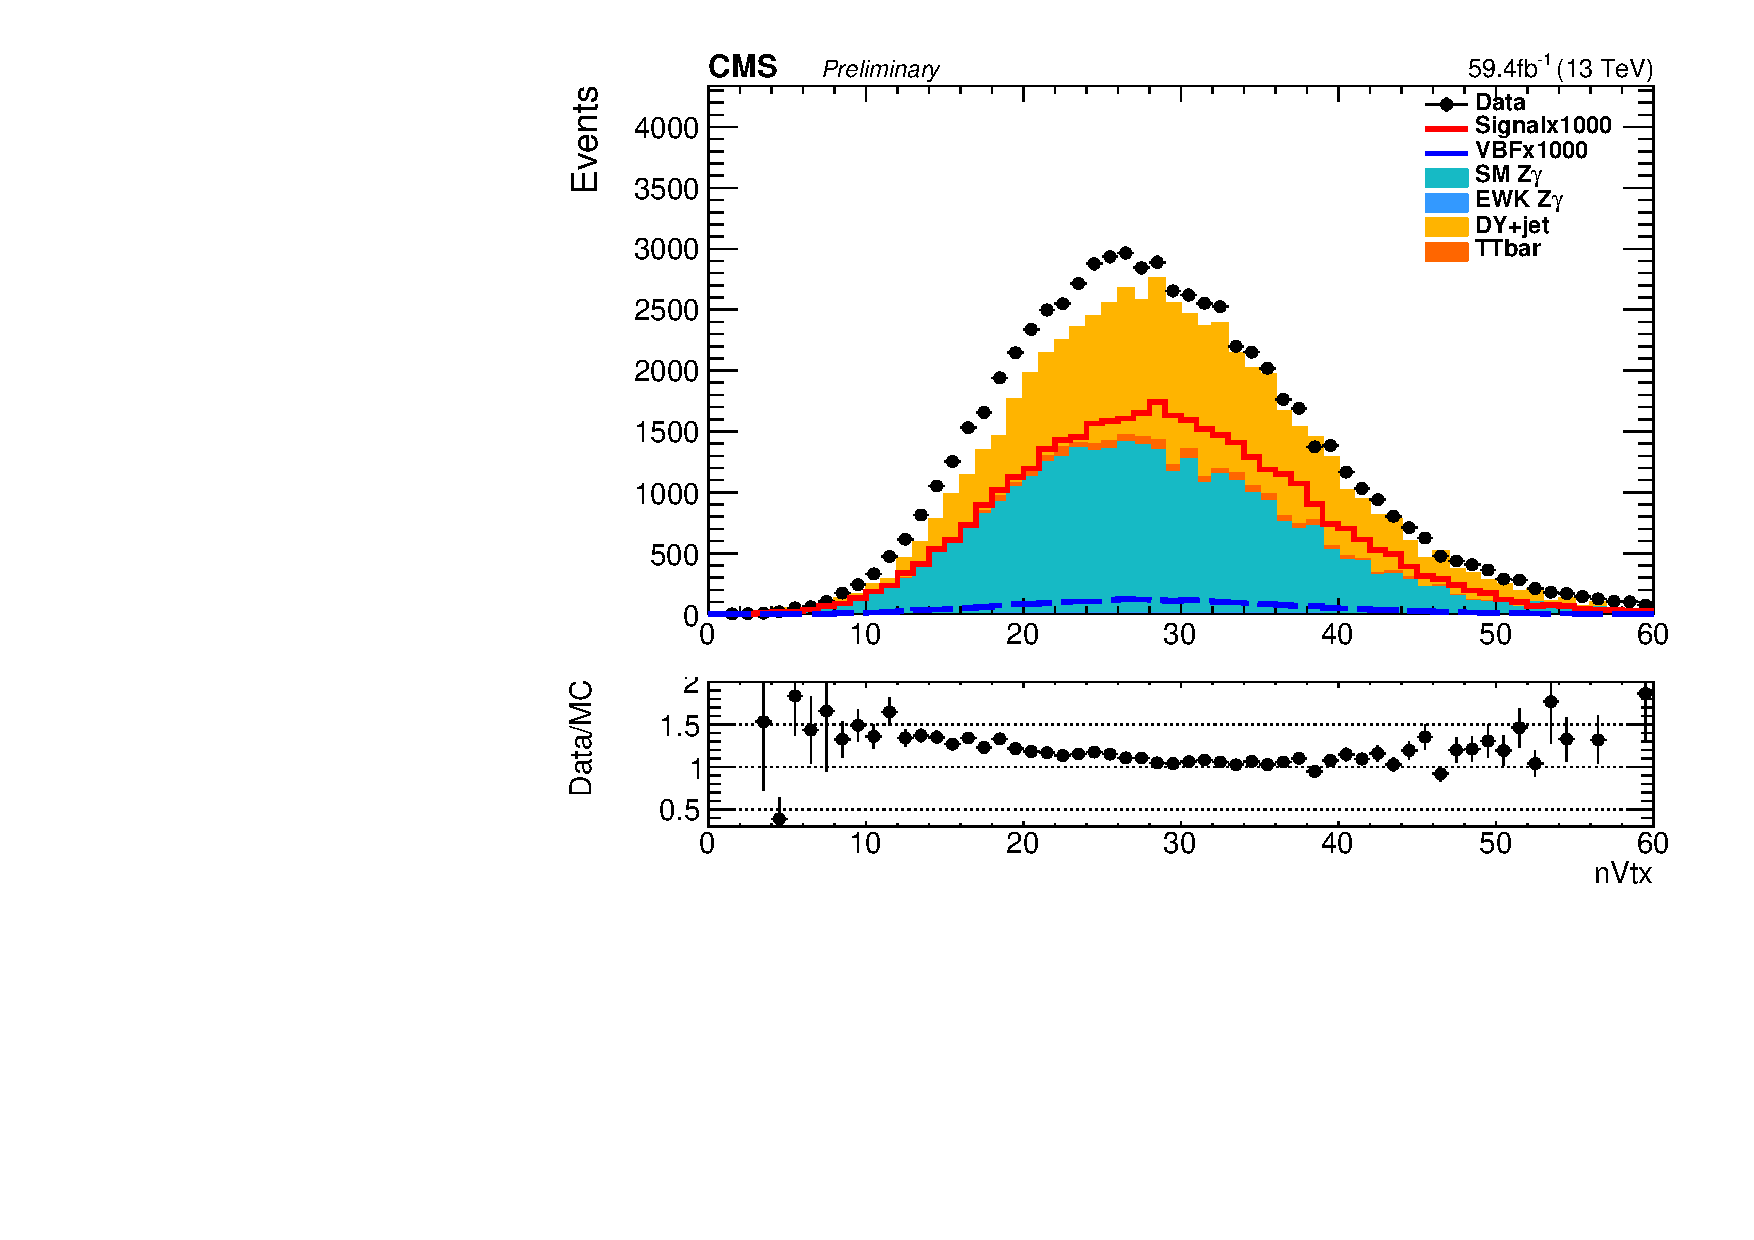
\includegraphics[width=0.3\textwidth]{fig/pileup/ele_kin_nVtx_valid_Rereco18_HLT.pdf}
  \end{center}
\caption{Distribution of the number of primary vertices in data and simulation shown for the electron channel after 2 leptons and 1 photon are selected. Left to right: 2016, 2017, 2018. The pileup cross section is taken to be 66 mb, 72.4 mb, and 80 mb for 2016, 2017, and 2018 respectively.}
\label{fig:puwei}
\end{figure}

\section{Level-1 Trigger Prefiring Problem}\label{sec:L1}
In 2016 and 2017, a gradual timing shift of the ECAL was not properly propagated to 
L1 trigger primitives (TP) resulting in a significant fraction of high eta TP 
being mistakenly associated to the previous bunch crossing. 
Since Level 1 rules forbid two consecutive bunch crossings to fire, 
an unpleasant consequence of this (in addition to not finding the TP in the bx 0) 
is that events can self veto if a significant amount of ECAL energy is found in the region 
of $2.<|\eta|<3$. This effect is not described by the simulations \cite{L1_prefire}.\\

The JETMET twiki provides a recipe to compute the probability for an event not to prefire, that can then be applied to the simulations. This is achieved with an EDProducer that runs over all offline photons and jets found in the event and assign them a prefiring probability. 

The final event weight is obtained as the product of the non prefiring probability of all objects (measured using unprefirable events), namely:
\begin{equation}
	\omega = 1 - P(Prefiring) = \prod_{i=photon,jets}(1-\epsilon_i^{pref}(\eta,\pt^{EM}))
\end{equation}

The impact of the L1 prefiring for electrons (muons) is a 1.4 (0.8)\% 
loss in signal yield for 2016 and 2.4 (1.1)\% 
loss in signal yield for 2017.



\chapter{Physics Object and Event Selection}\label{sec:selection}
This chapter outlines the basic \hzg{} physics object and event selection before any event categorization is done.
Along the way, we will also point out the most relevant corrections applied, including trigger scale factors (SFs), physics object energy and momentum corrections, and identification and isolation SFs.

\section{Primary Vertex}
Events are required to have at least one good PV
with a reconstructed longitudinal position within 24\cm of the
geometric center of the detector and a transverse position within
2\cm of the nominal beam collision point. 
To avoid fake vertices, the PV reconstruction is required to have more than four degrees of freedom.
In the case of multiple satisfactory vertices, the vertex with the highest scalar sum of squared \pt is chosen.

\section{Triggers}
The topology and kinematics of the \hzg{} process guide the choice of triggers used in this analysis. As there are at least three final state decay products, 
the photon \pt tends to be less than in other channels, such as \hgg. Consequently, the CMS single photon trigger \pt thresholds 
are too great to make them viable options. In addition, there is no suitable unprescaled multijet plus photon trigger to target events with 
hadronic decays of the $\PZ$ boson, so the triggers are chosen to target the $\lplm\gamma$ final states.
Therefore, we trigger on the leptons arising from the decay of the Z boson, which tend 
to have larger values of \pt. The best approach to maximize signal efficiency is to use the double lepton triggers. 
The dielectron trigger requires a leading (subleading) electron with
$\pt > 23\,(12)\GeV$, while the dimuon trigger requires a muon with $\pt > 17\,(8)\GeV$. Events passing both the double muon and double electron triggers are classified as $\mpmm\gamma$ events.

The triggers are applied to both data and simulation. Trigger efficiencies and SFs are measured using the 
simulation samples corresponding to each data-taking year. These measurements use a tag and probe~\cite{cite:tagandprobe} method. 
This method takes advantage of the high purity of $\PZ\to\lplm$ events near the $\PZ$ boson mass peak. 
One lepton functions as the tag, and satisfies a set of tight trigger, identification, isolation, and \pt requirements. 
The second lepton, the probe, must pass a looser selection and is used to measure the efficiency in question. 
Using this approach, trigger efficiencies for each leg of a given double lepton trigger are measured in both data and simulation. 
Then a corrective SF, defined as the ratio of data efficiency to simulation efficiency, is applied to the simulation. 
Scale factors are measured and applied in bins of \pt and $|\eta|$.

For the double electron trigger efficiency measurements, the tag electron must satisfy a set of requirements. The tag must pass 
the single electron trigger, pass a tight cut-based identification, have $\pt>30\,(35)\GeV$ in 2016 (2017 and 2018), and have $|\eta|<2.5$. 
The probe electron must pass a loose electron MVA identification requirement. The details of the electron MVA identification will be described later in this chapter.
The efficiencies for each leg 
of the trigger are measured separately, so in each case, the probe electron must match the trigger leg being measured. 
The efficiencies for each double electron trigger leg for 2016, 2017, and 2018 are shown in Fig. \ref{fig:ele_trig_SF}.
On average, the double electron trigger efficiency is measured to be in the range of 86--97\%, depending on the electron \pt and $\eta$.

\begin{figure}[tb]
	\begin{center}
		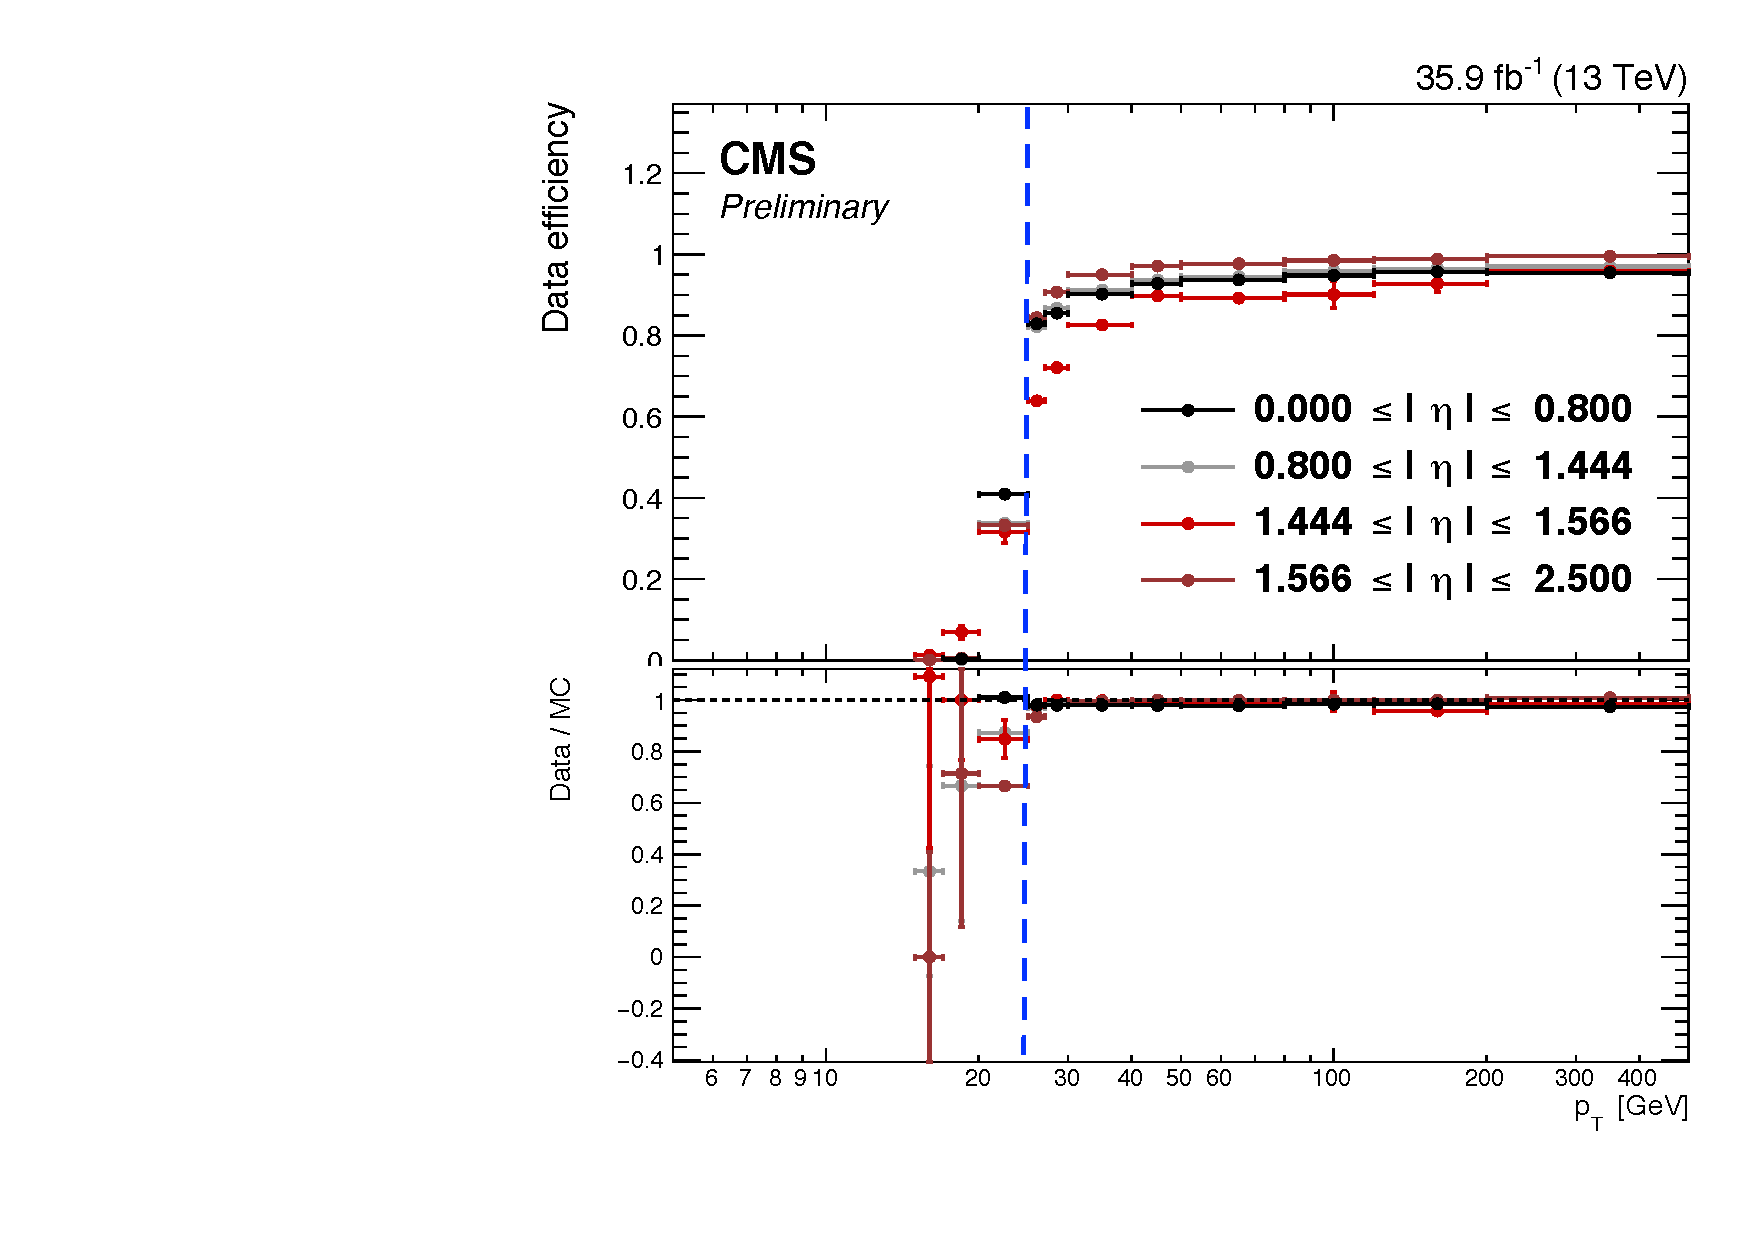
\includegraphics[width=0.30\textwidth]{fig/SFs/2016_ele_trg1_1D.pdf}
		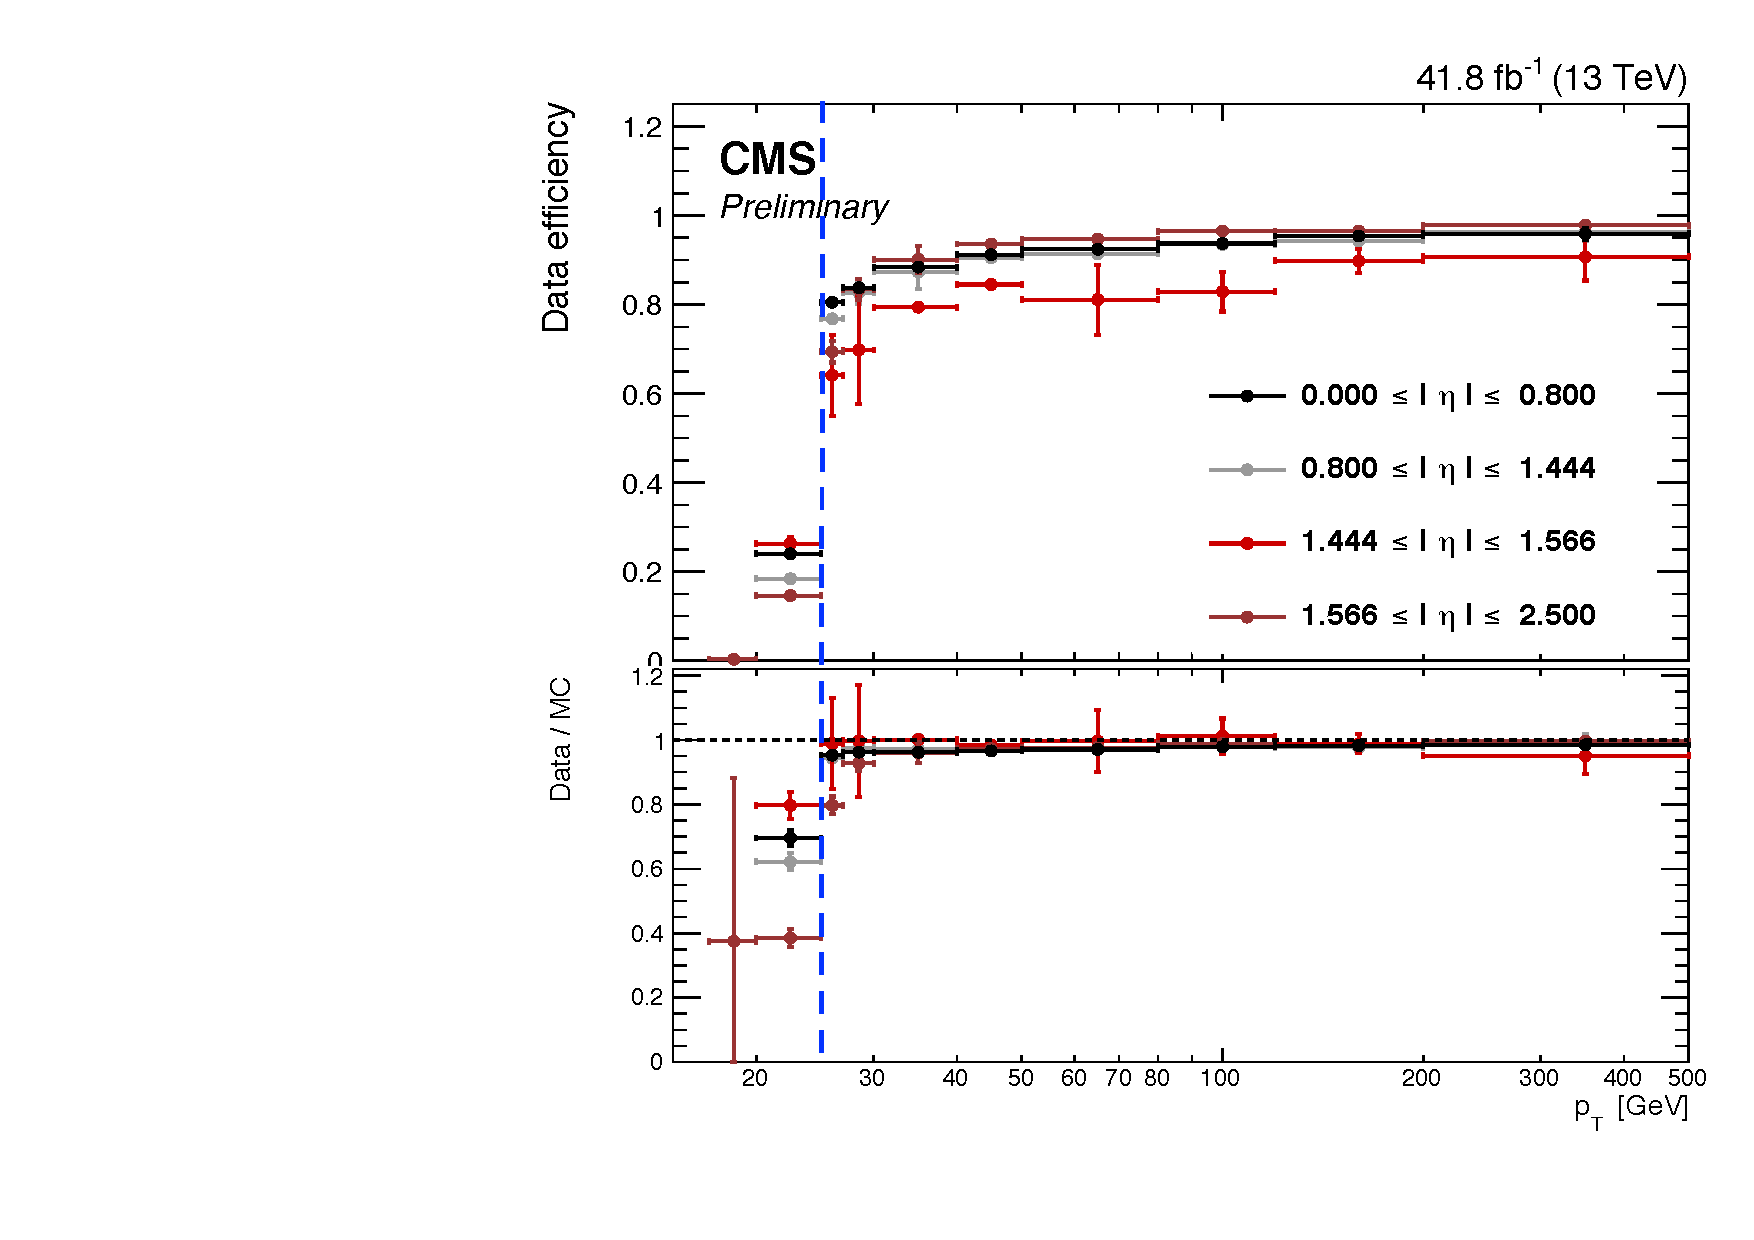
\includegraphics[width=0.30\textwidth]{fig/SFs/2017_ele_trg1_1D.pdf}
		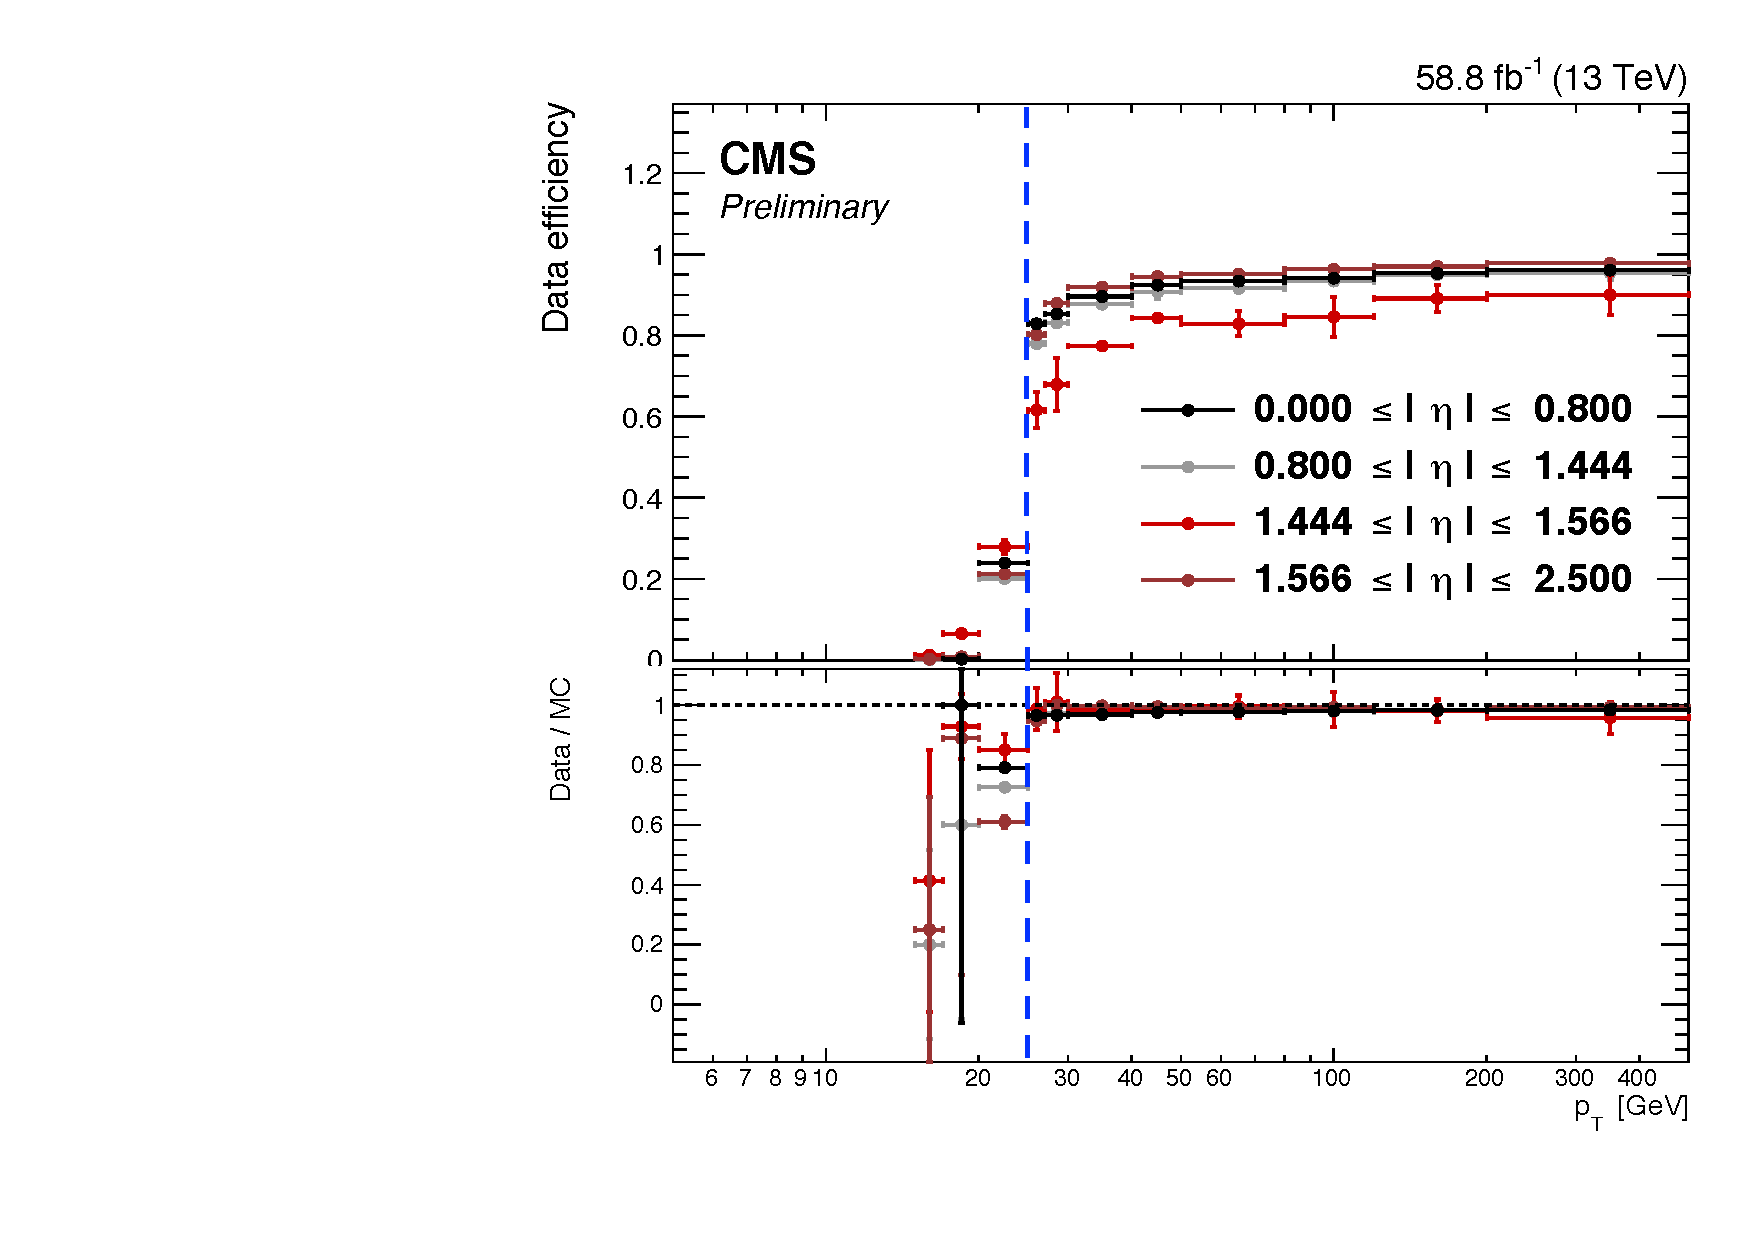
\includegraphics[width=0.30\textwidth]{fig/SFs/2018_ele_trg1_1D.pdf}
		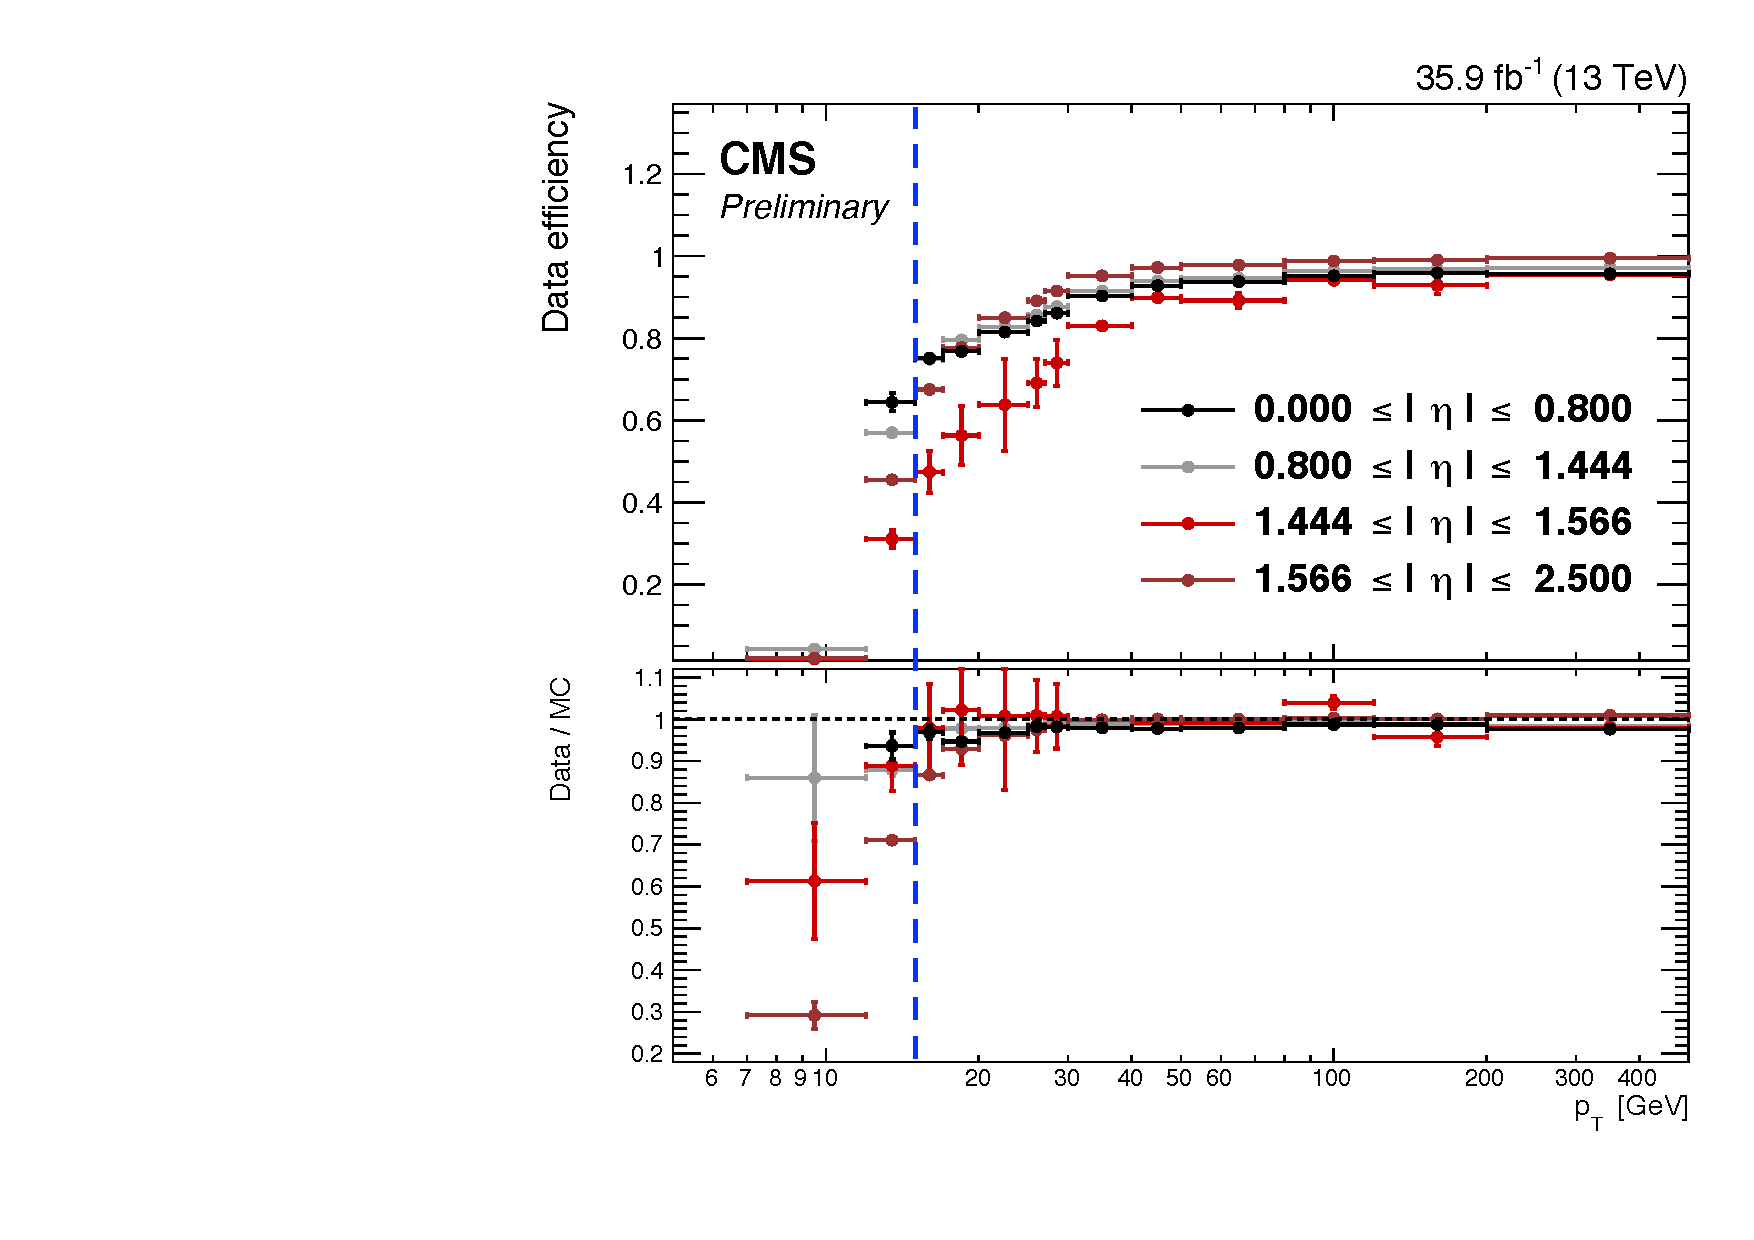
\includegraphics[width=0.30\textwidth]{fig/SFs/2016_ele_trg2_1D.pdf}
		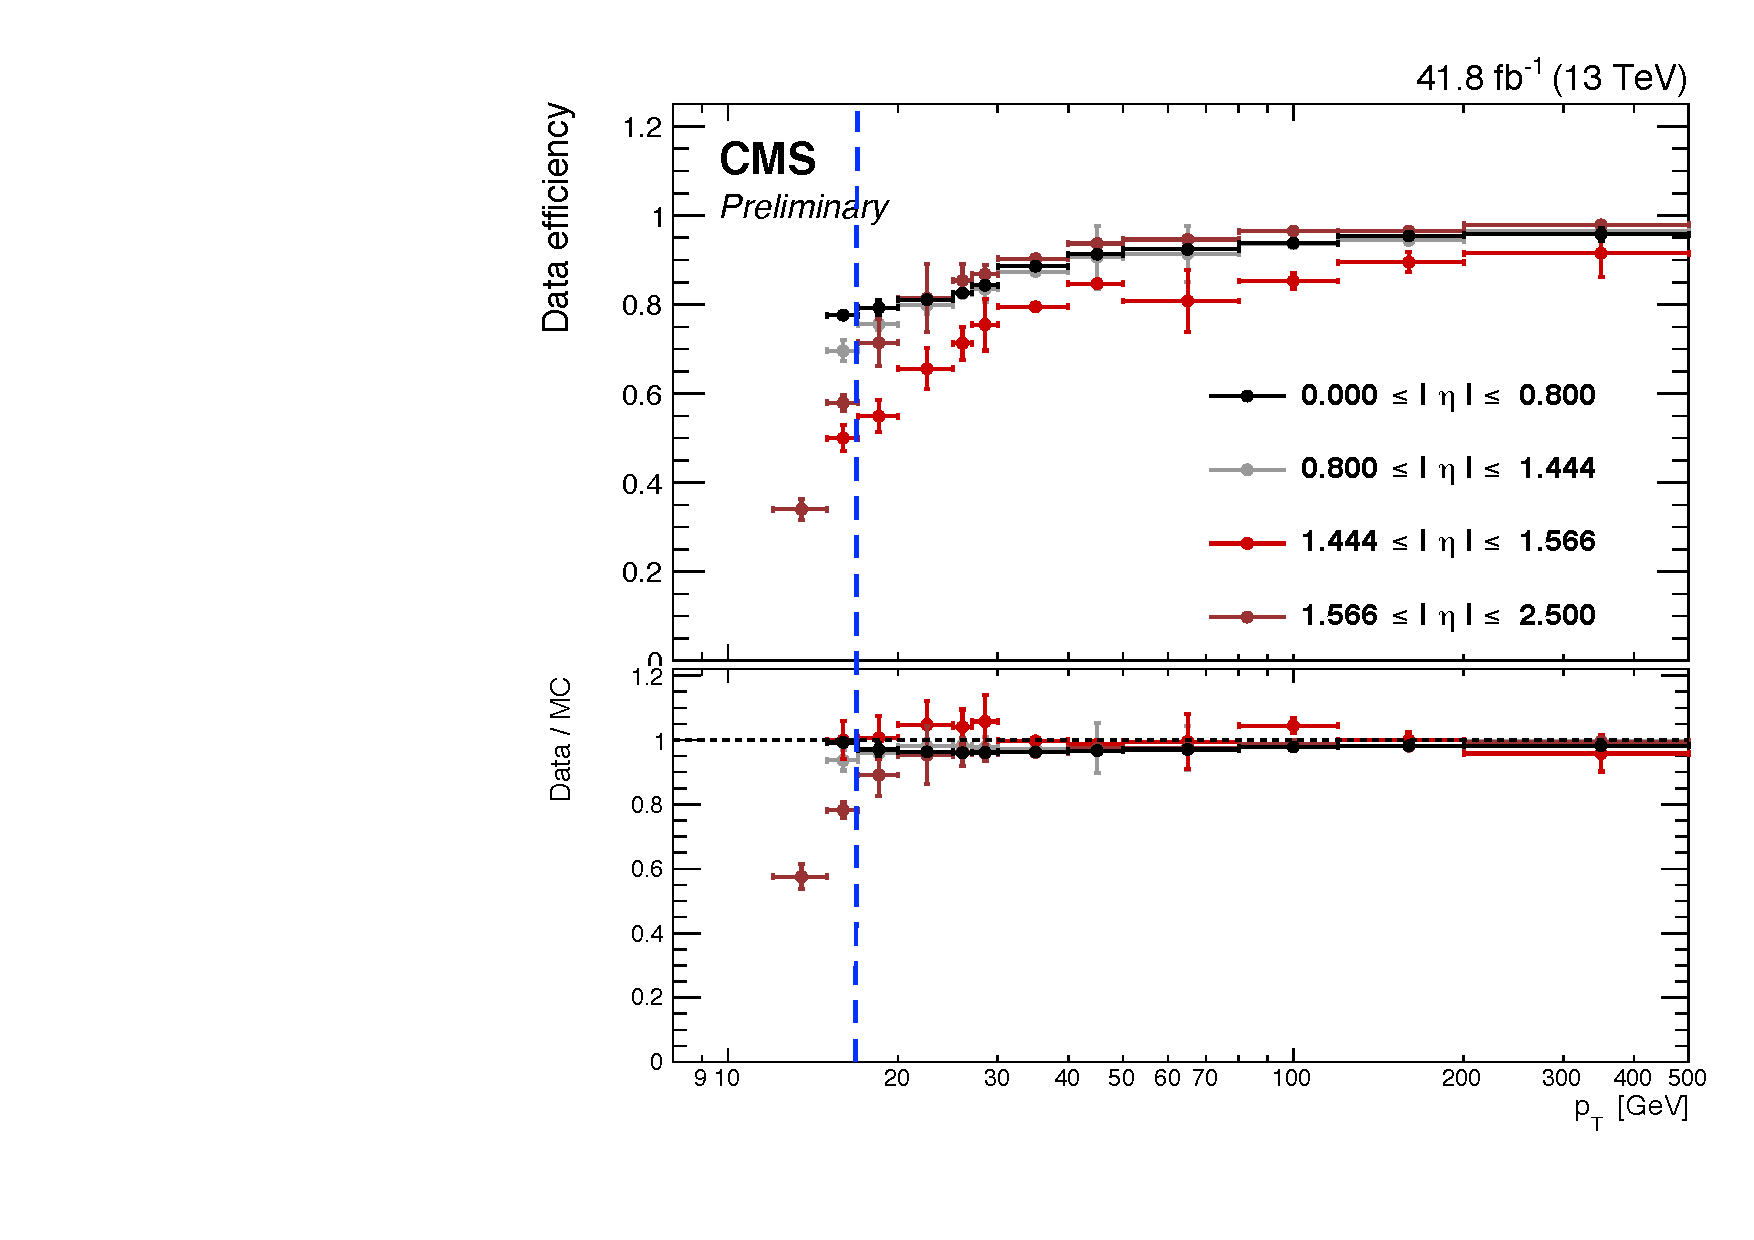
\includegraphics[width=0.30\textwidth]{fig/SFs/2017_ele_trg2_1D.pdf}
		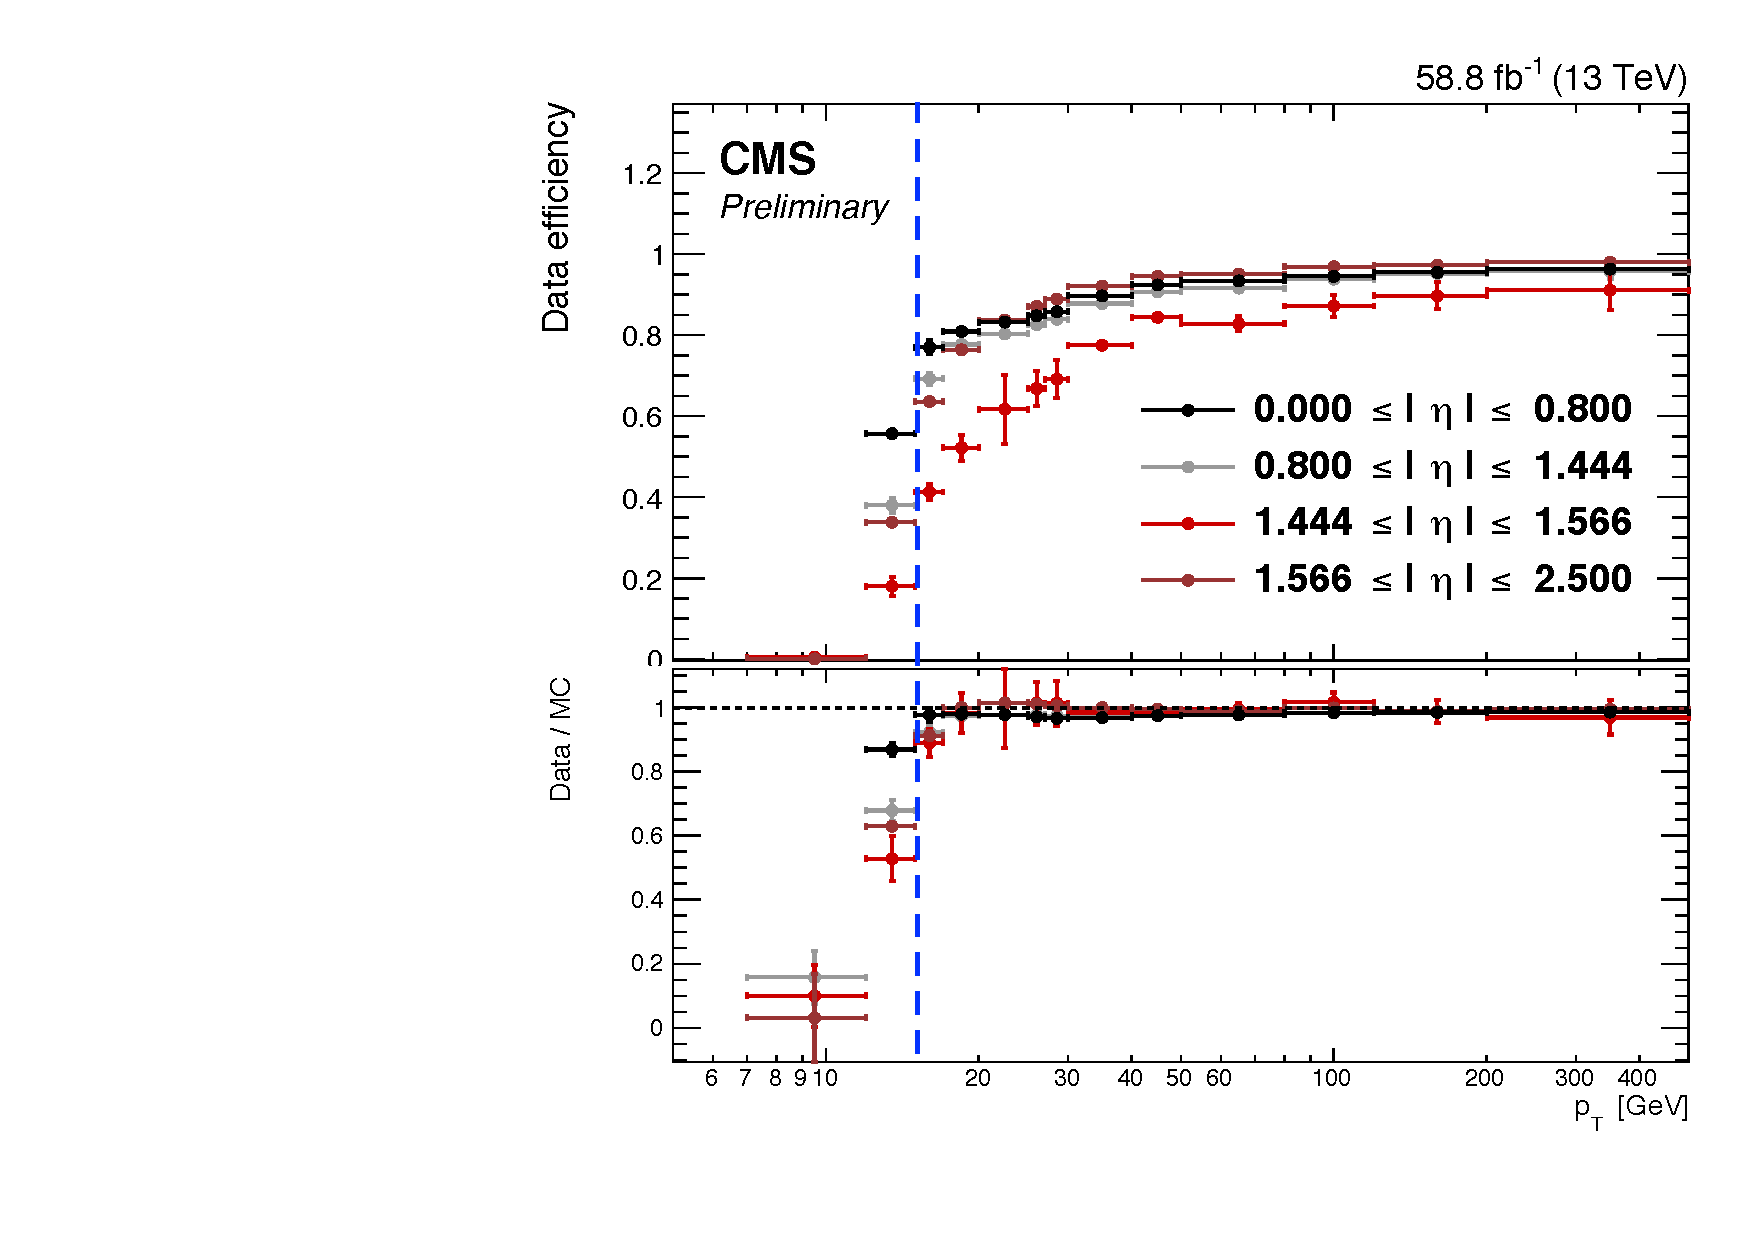
\includegraphics[width=0.30\textwidth]{fig/SFs/2018_ele_trg2_1D.pdf}
	\end{center}
	\caption{Efficiency measurements for each leg of the double electron trigger in 2016 (left), 2017 (center), and 2018 (right). The upper (lower) plots correspond to the 
	leading (subleading) trigger leg.}
	\label{fig:ele_trig_SF}
\end{figure}

For the double muon trigger efficiency measurements, the tag muon must satisfy a set of requirements. It must pass the single 
muon trigger, pass a tight cut-based identification, have $\pt>26\,(29)$ GeV for 2016 (2017 and 2018) and satisfy $|\eta| < 2.4$. The 
probe muon must pass the $\PH\to\PZ\PZ$ identification and isolation cuts. The details of the $\PH\to\PZ\PZ$ muon 
identification will be described later in this chapter. The efficiencies for each leg of the trigger are measured separately, so in each case, the probe 
muon must match the trigger leg being measured. The efficiencies for each double muon trigger leg for 2016, 2017, 
and 2018 are shown in Fig. \ref{fig:mu_trig_SF}. On average, the double muon trigger efficiency is measured to be in the range of 93--95\%, depending on the muon \pt and $\eta$.

\begin{figure}[tb]
	\begin{center}
		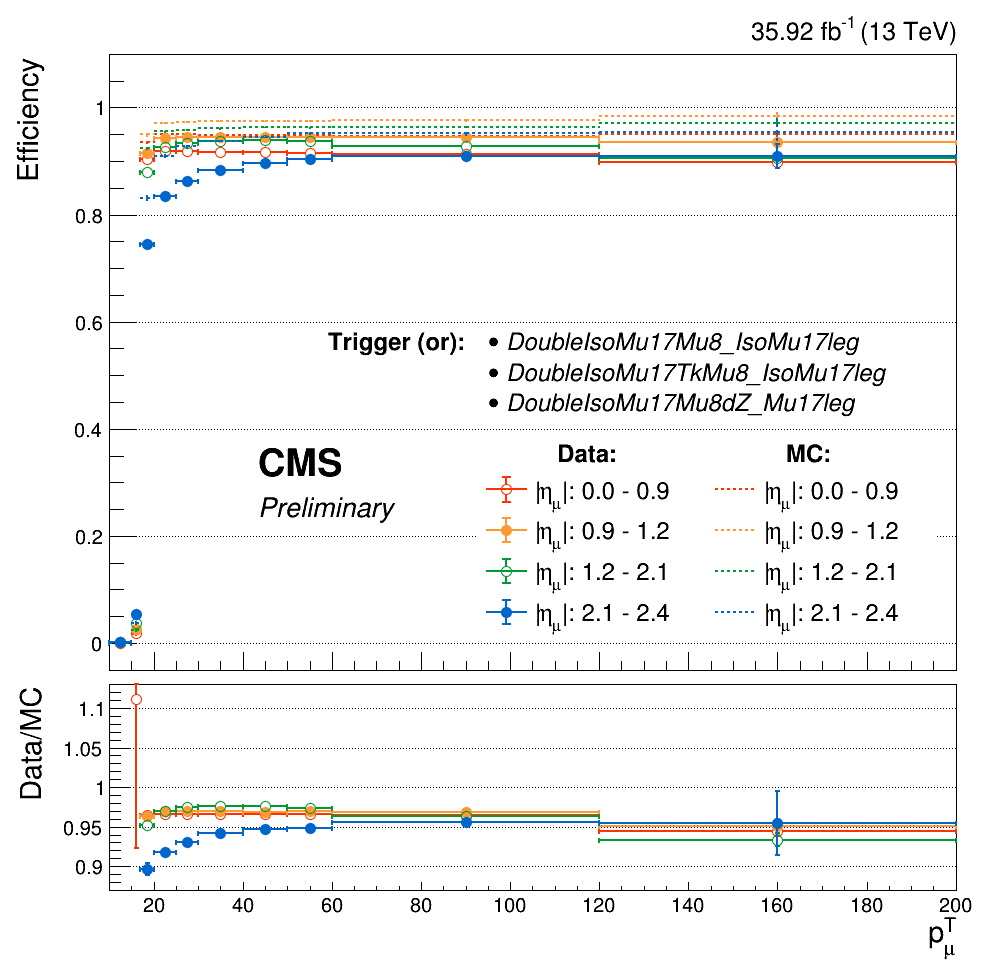
\includegraphics[width=0.30\textwidth]{fig/SFs/sf1D_year2016_leg1.png}
		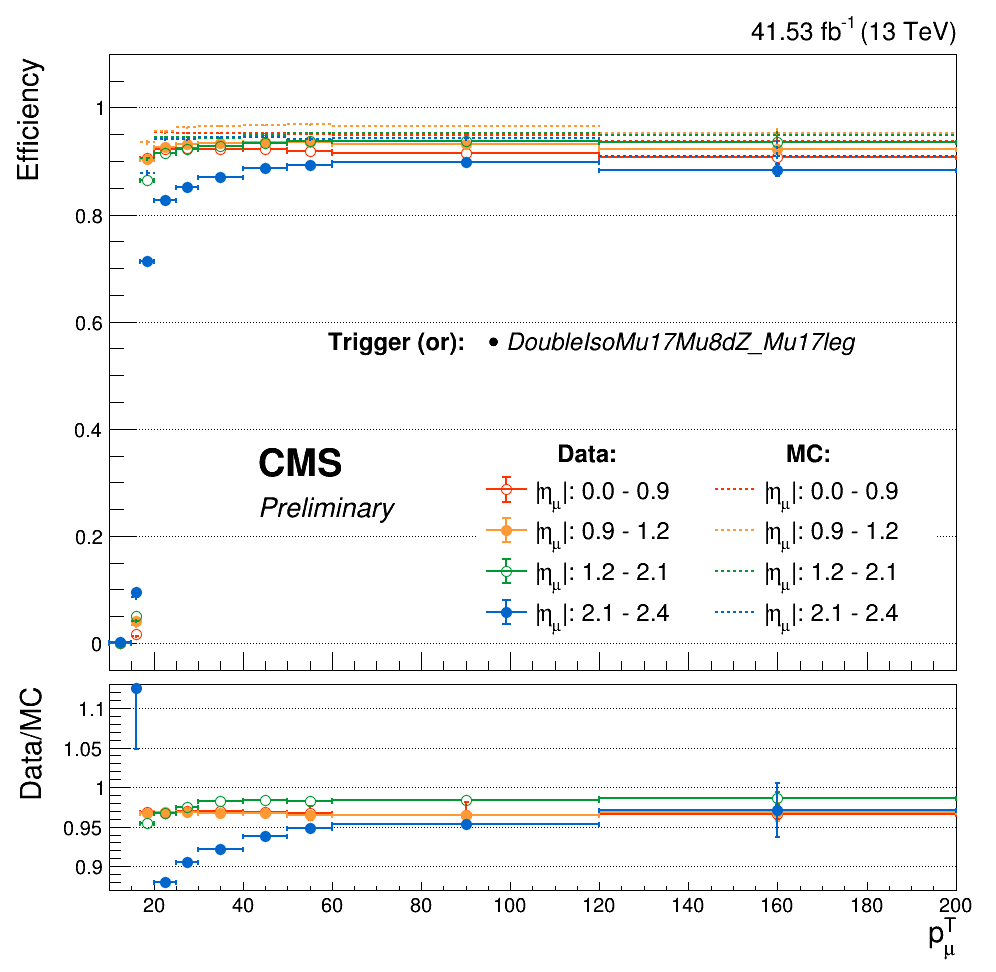
\includegraphics[width=0.30\textwidth]{fig/SFs/sf1D_year2017_leg1.png}
		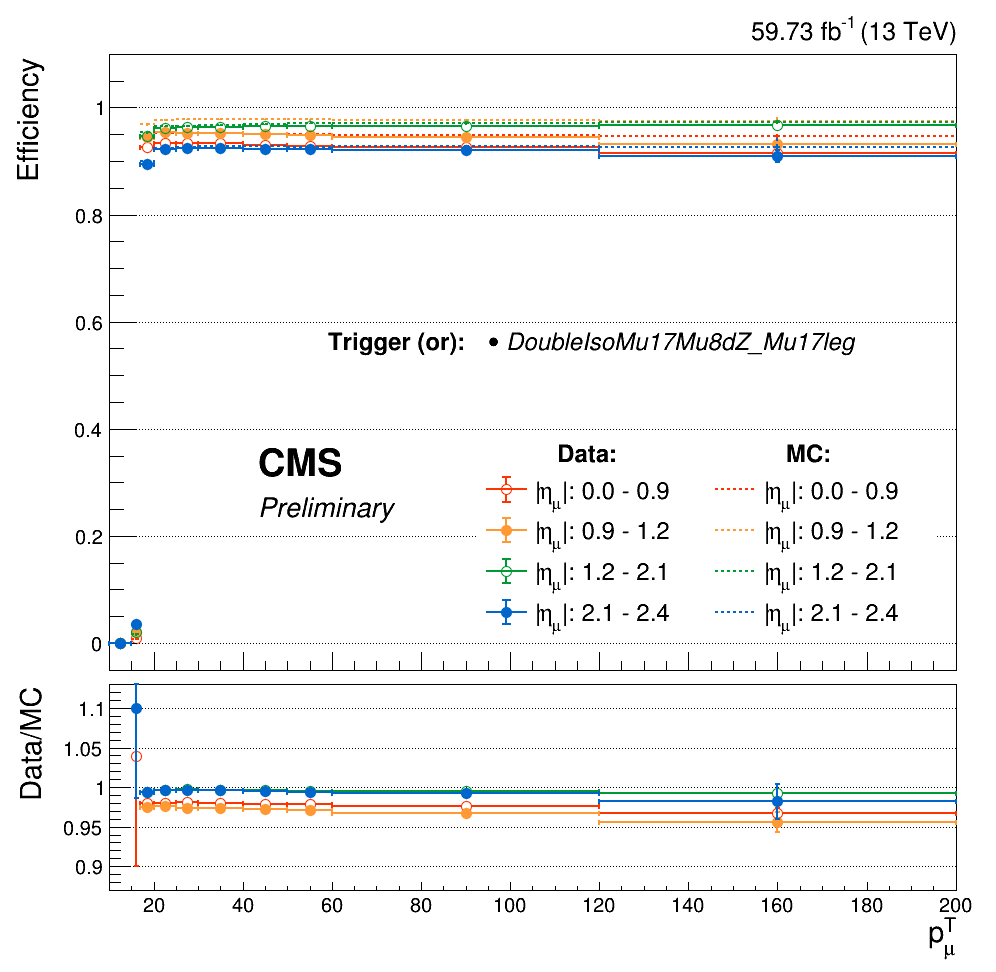
\includegraphics[width=0.30\textwidth]{fig/SFs/sf1D_year2018_leg1.png}
		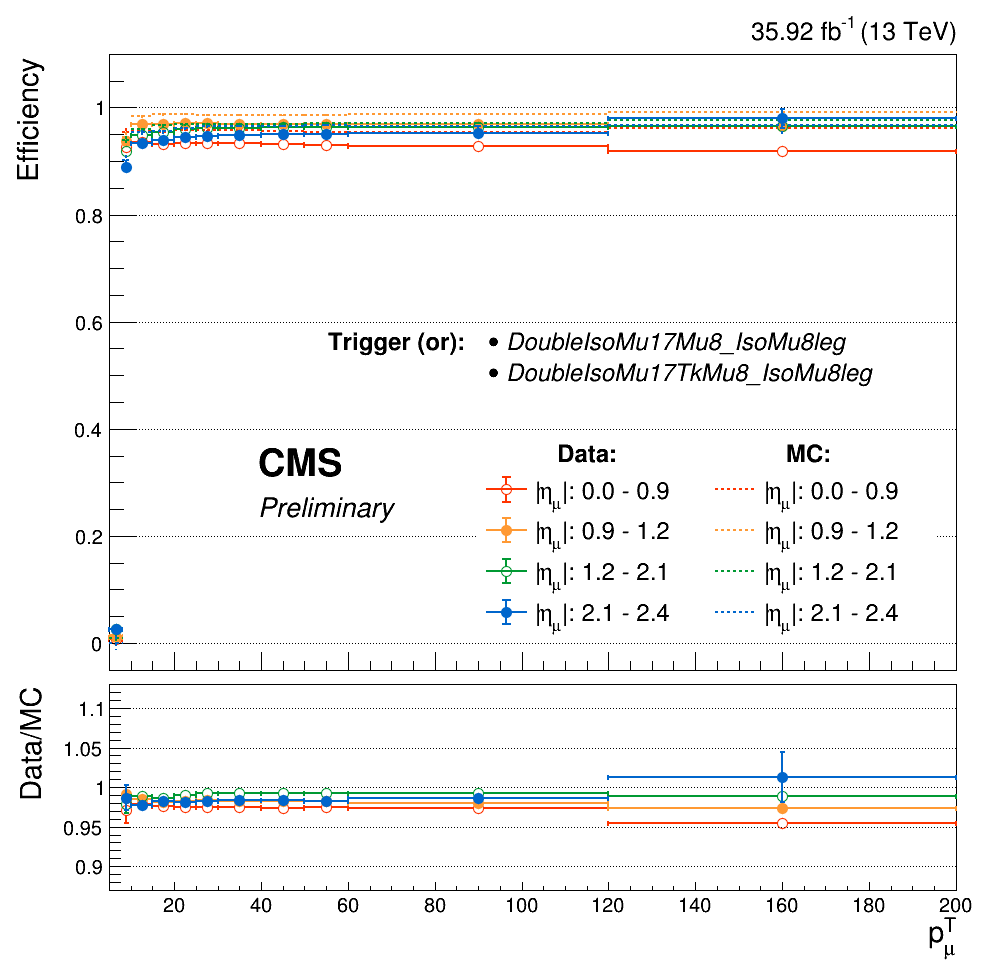
\includegraphics[width=0.30\textwidth]{fig/SFs/sf1D_year2016_leg2.png}
		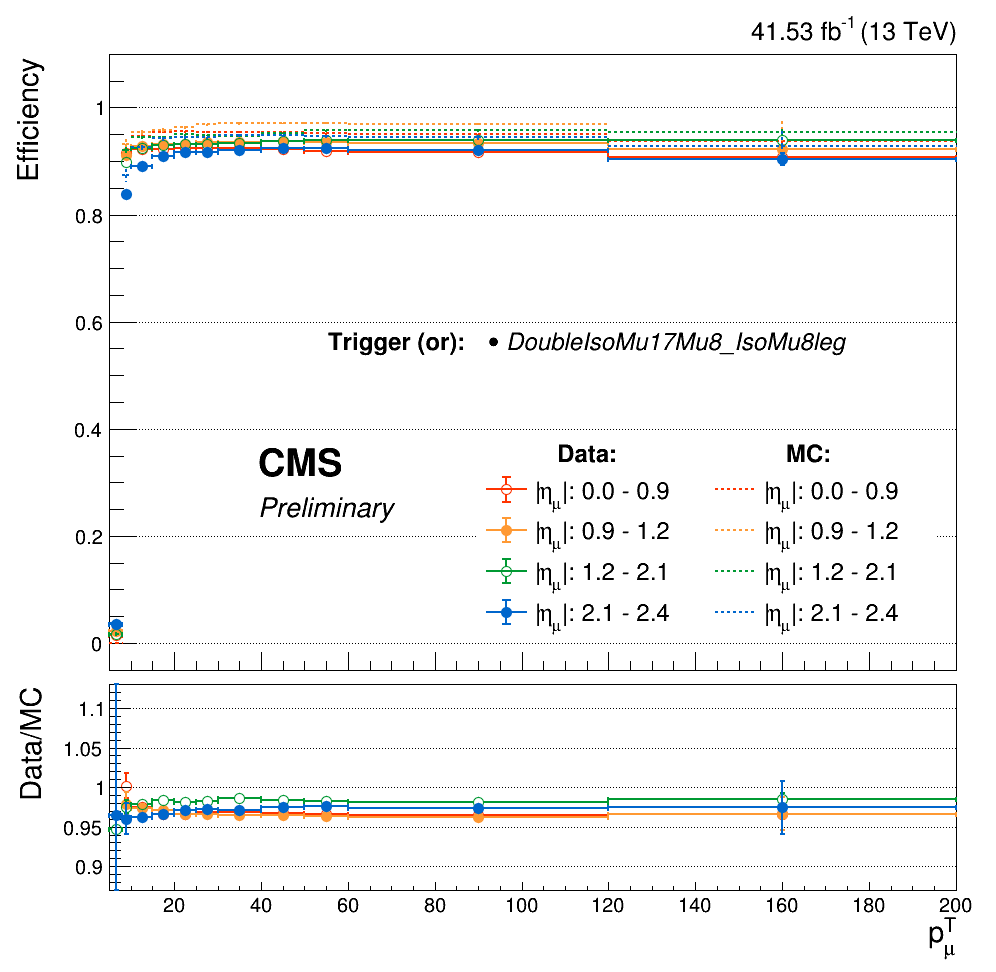
\includegraphics[width=0.30\textwidth]{fig/SFs/sf1D_year2017_leg2.png}
		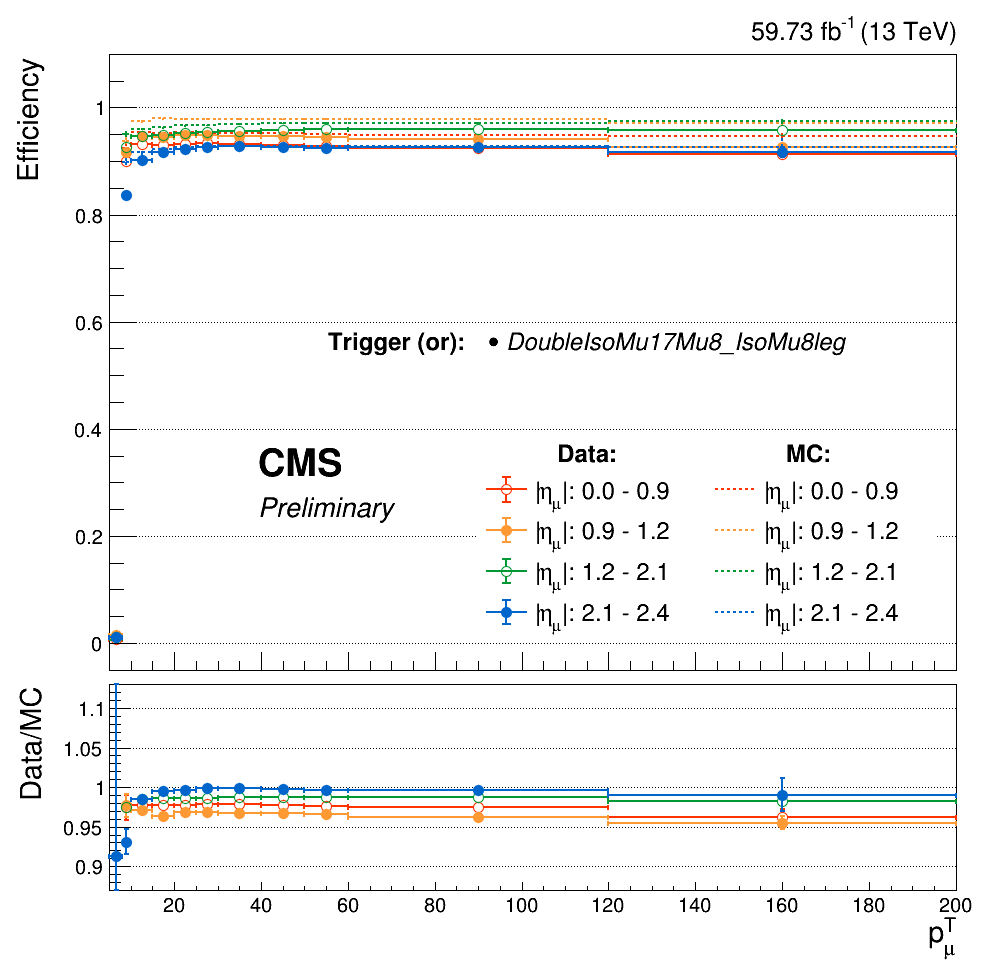
\includegraphics[width=0.30\textwidth]{fig/SFs/sf1D_year2018_leg2.png}
	\end{center}
	\caption{Efficiency measurements for each leg of the double muon trigger in 2016 (left), 2017 (center), and 2018 (right). The upper (lower) plots correspond to the 
	leading (subleading) trigger leg.}
	\label{fig:mu_trig_SF}
\end{figure}

\section{Photon Selection}
Photons are identified using a BDT discriminant (photon MVA ID) trained on $\PGg$+jets simulation in order to distinguish real photons from jets misreconstructed as photons. 
The features used for the BDT training include supercluster kinematics, isolation variables, and shower shape variables~\cite{EGM:PhotonID}. 
To reject electrons faking photons, a conversion-safe electron veto is also applied. In order to improve agreement between simulation and data for the photon MVA ID, shower 
shape corrections are taken from the CMS $\PH\to\PGg\PGg$ analysis of the same data set~\cite{CMS:2021kom} and applied to simulated events. 
The photon MVA ID is then reevaluated after these corrections. We correct the following features: $R_{9}^{5x5}$, defined as the ratio of energy in
the 5x5 array of ECAL crystals to the supercluster energy; $S_{4}$, defined as the ratio of the maximum energy 2x2 array to the energy of 
the 5x5 array; the energy weighted shower widths $\sigma_{\eta}$ and $\sigma_{\phi}$; the energy weighted widths by crystal index 
$\sigma_{i\eta i\eta}$ and $\sigma_{i\eta i\phi}$; photon isolation, charged isolation with respect to the primary vertex, 
and charged isolation with respect to the worst vertex choice. The validity of the shower shape corrections is checked using tag 
and probe procedures for $\PZ\to\epem$ events where the probe electron mimics a photon and $\PZ\to\mpmm$
events with an FSR photon. Comparisons of the agreement between uncorrected and corrected simulation with data for the photon MVA ID are shown in 
Fig. \ref{fig:photon_mva_correction}. Similar plots for individual shower shape features can be found in Appendix \ref{sec:shower_shape}. 

\begin{figure}[tb]
	\begin{center}
		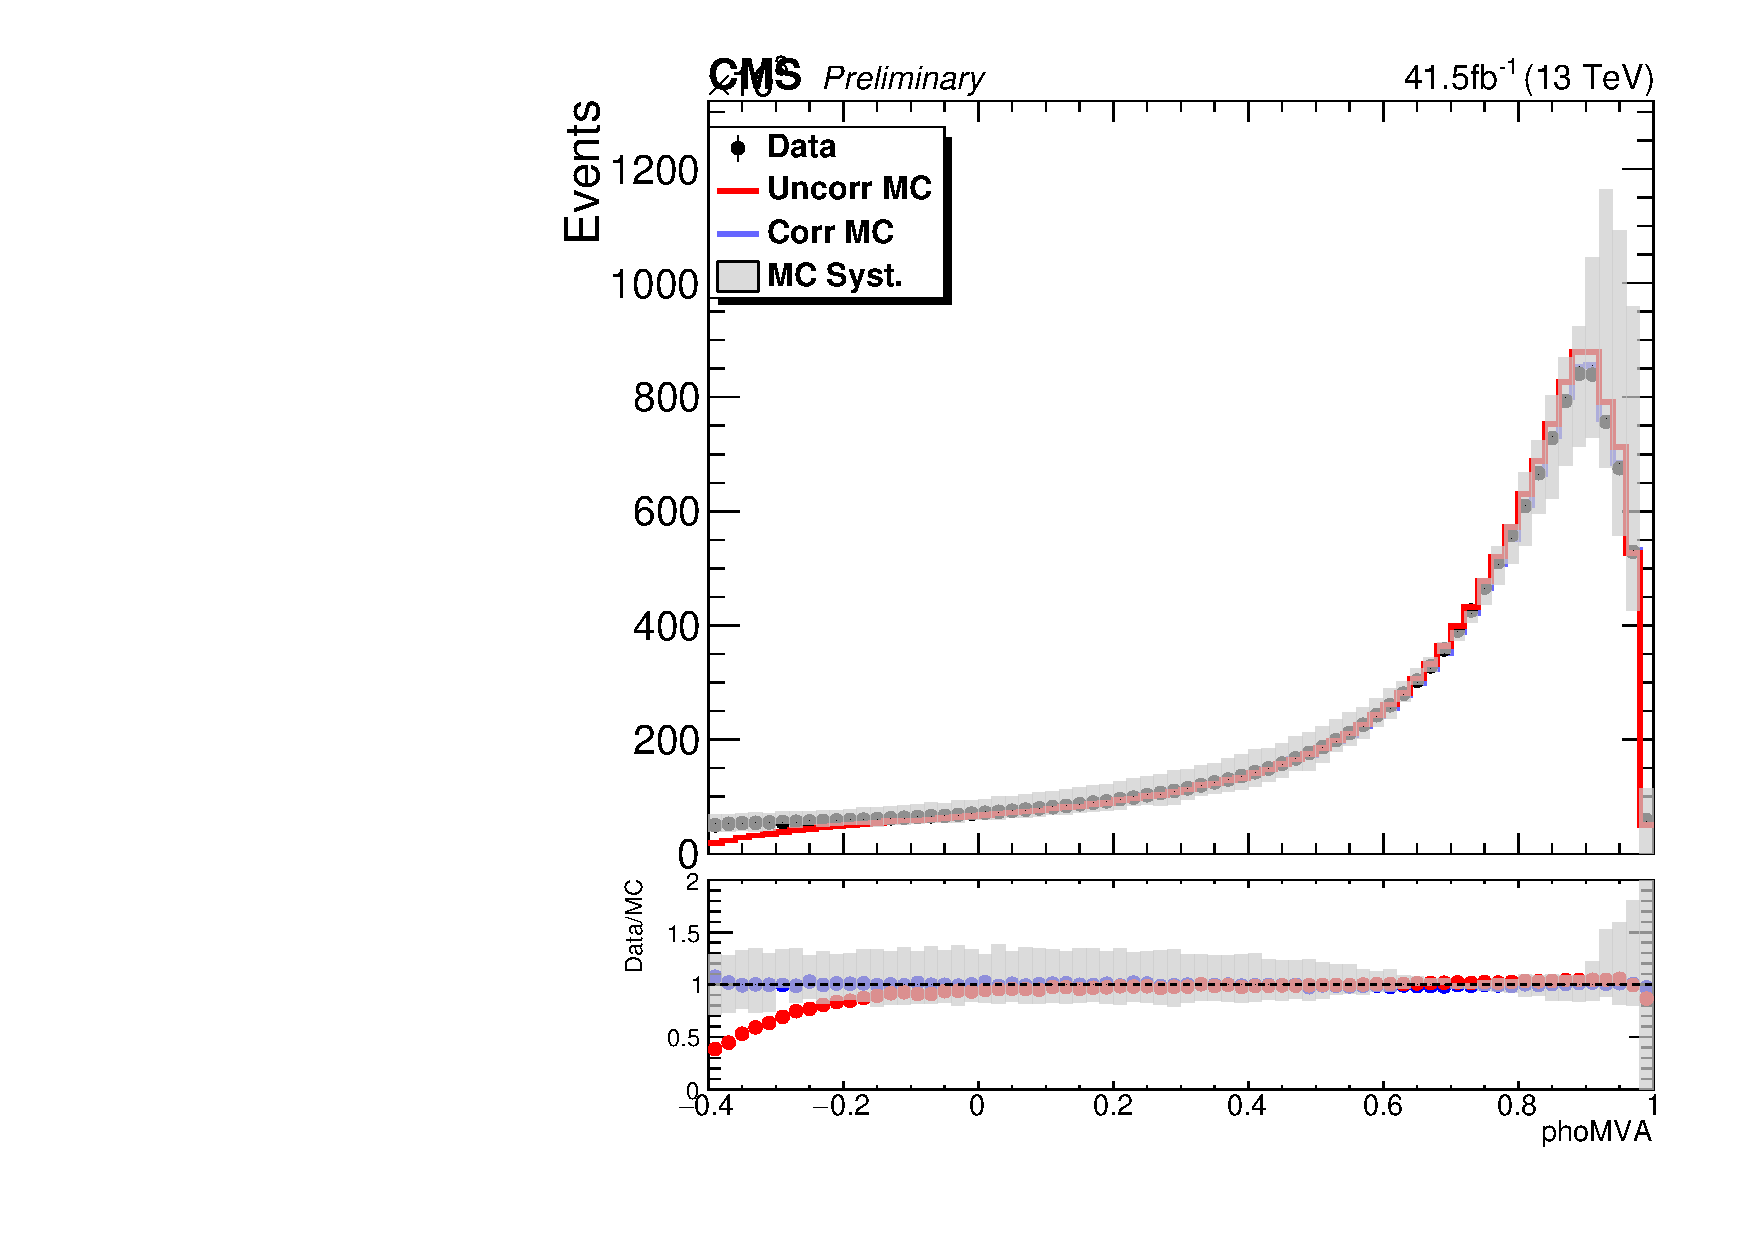
\includegraphics[width=0.35\textwidth]{fig/ss_corr/phoMVA_17_EB_Z.pdf}
		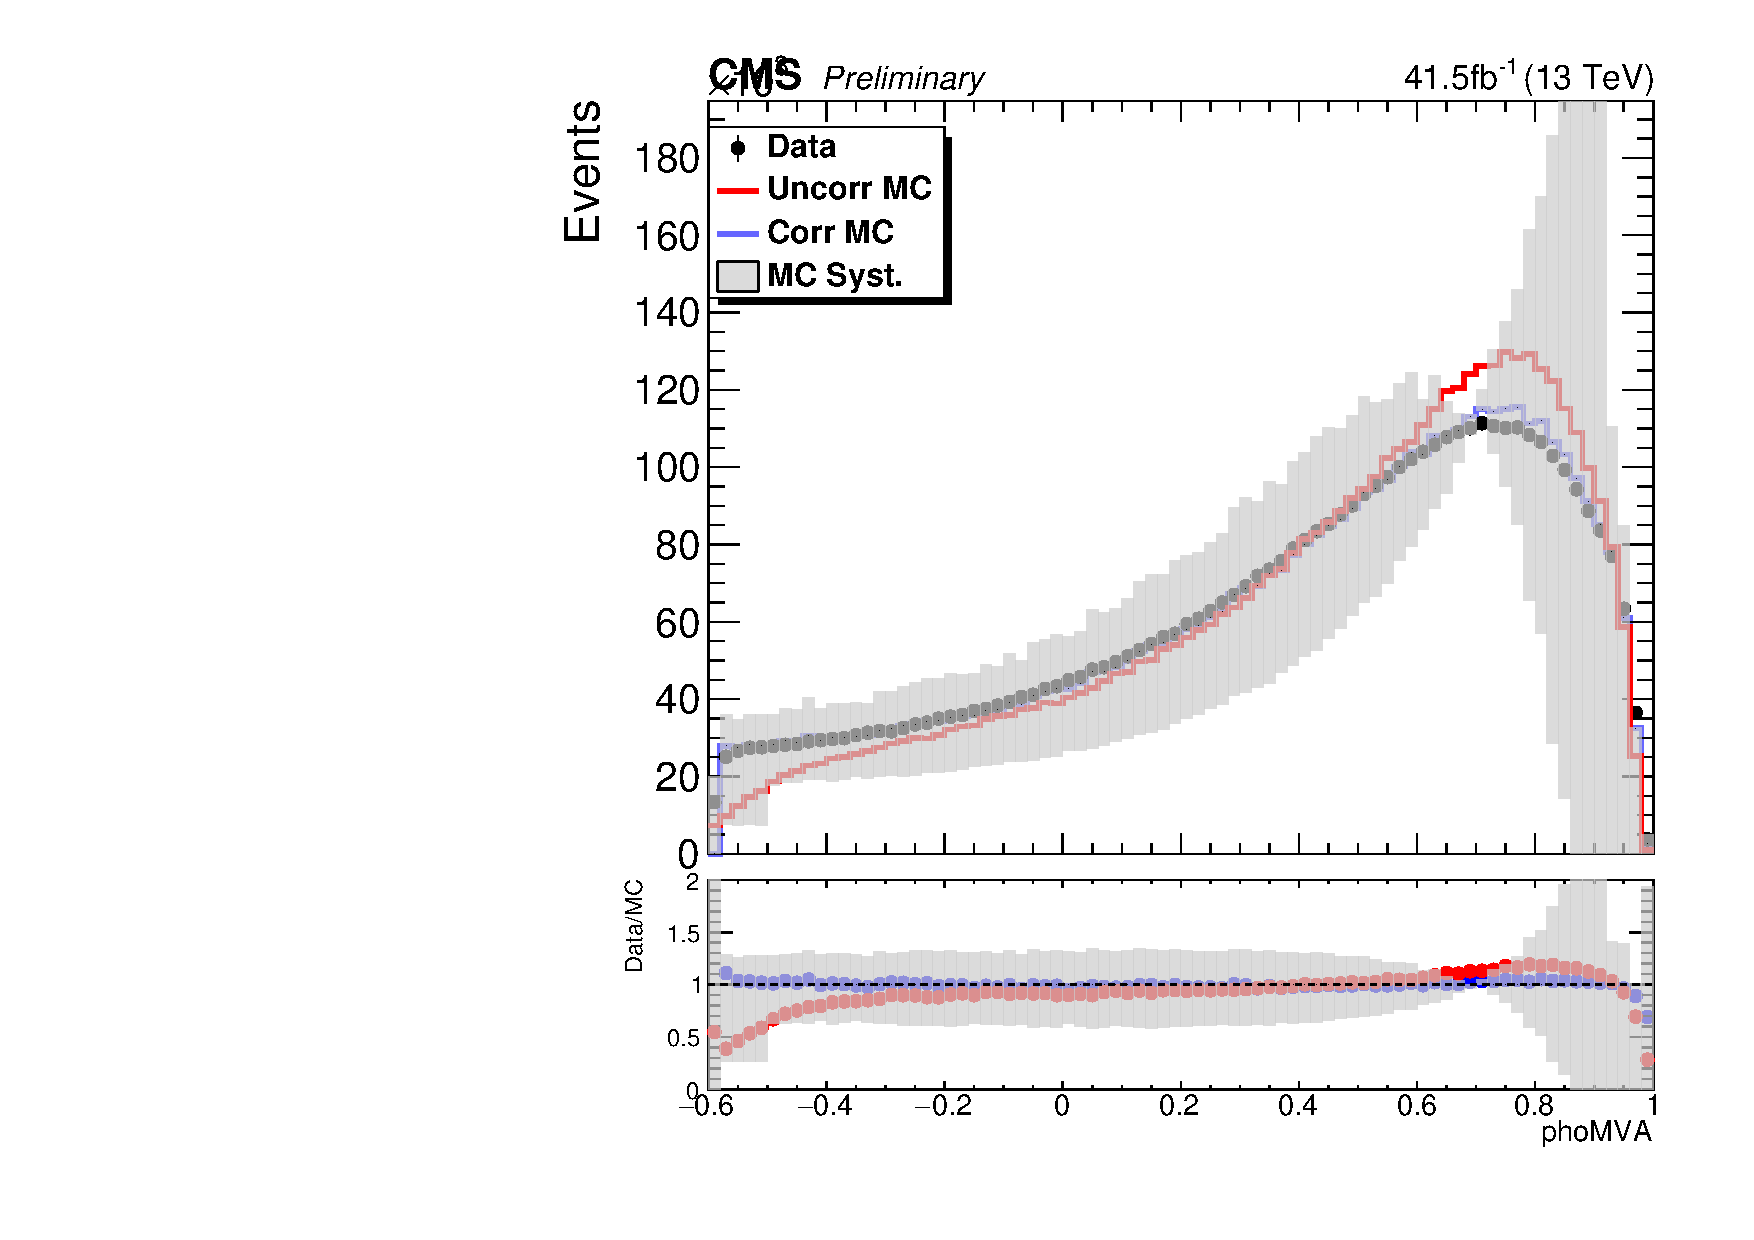
\includegraphics[width=0.35\textwidth]{fig/ss_corr/phoMVA_17_EE_Z.pdf}
		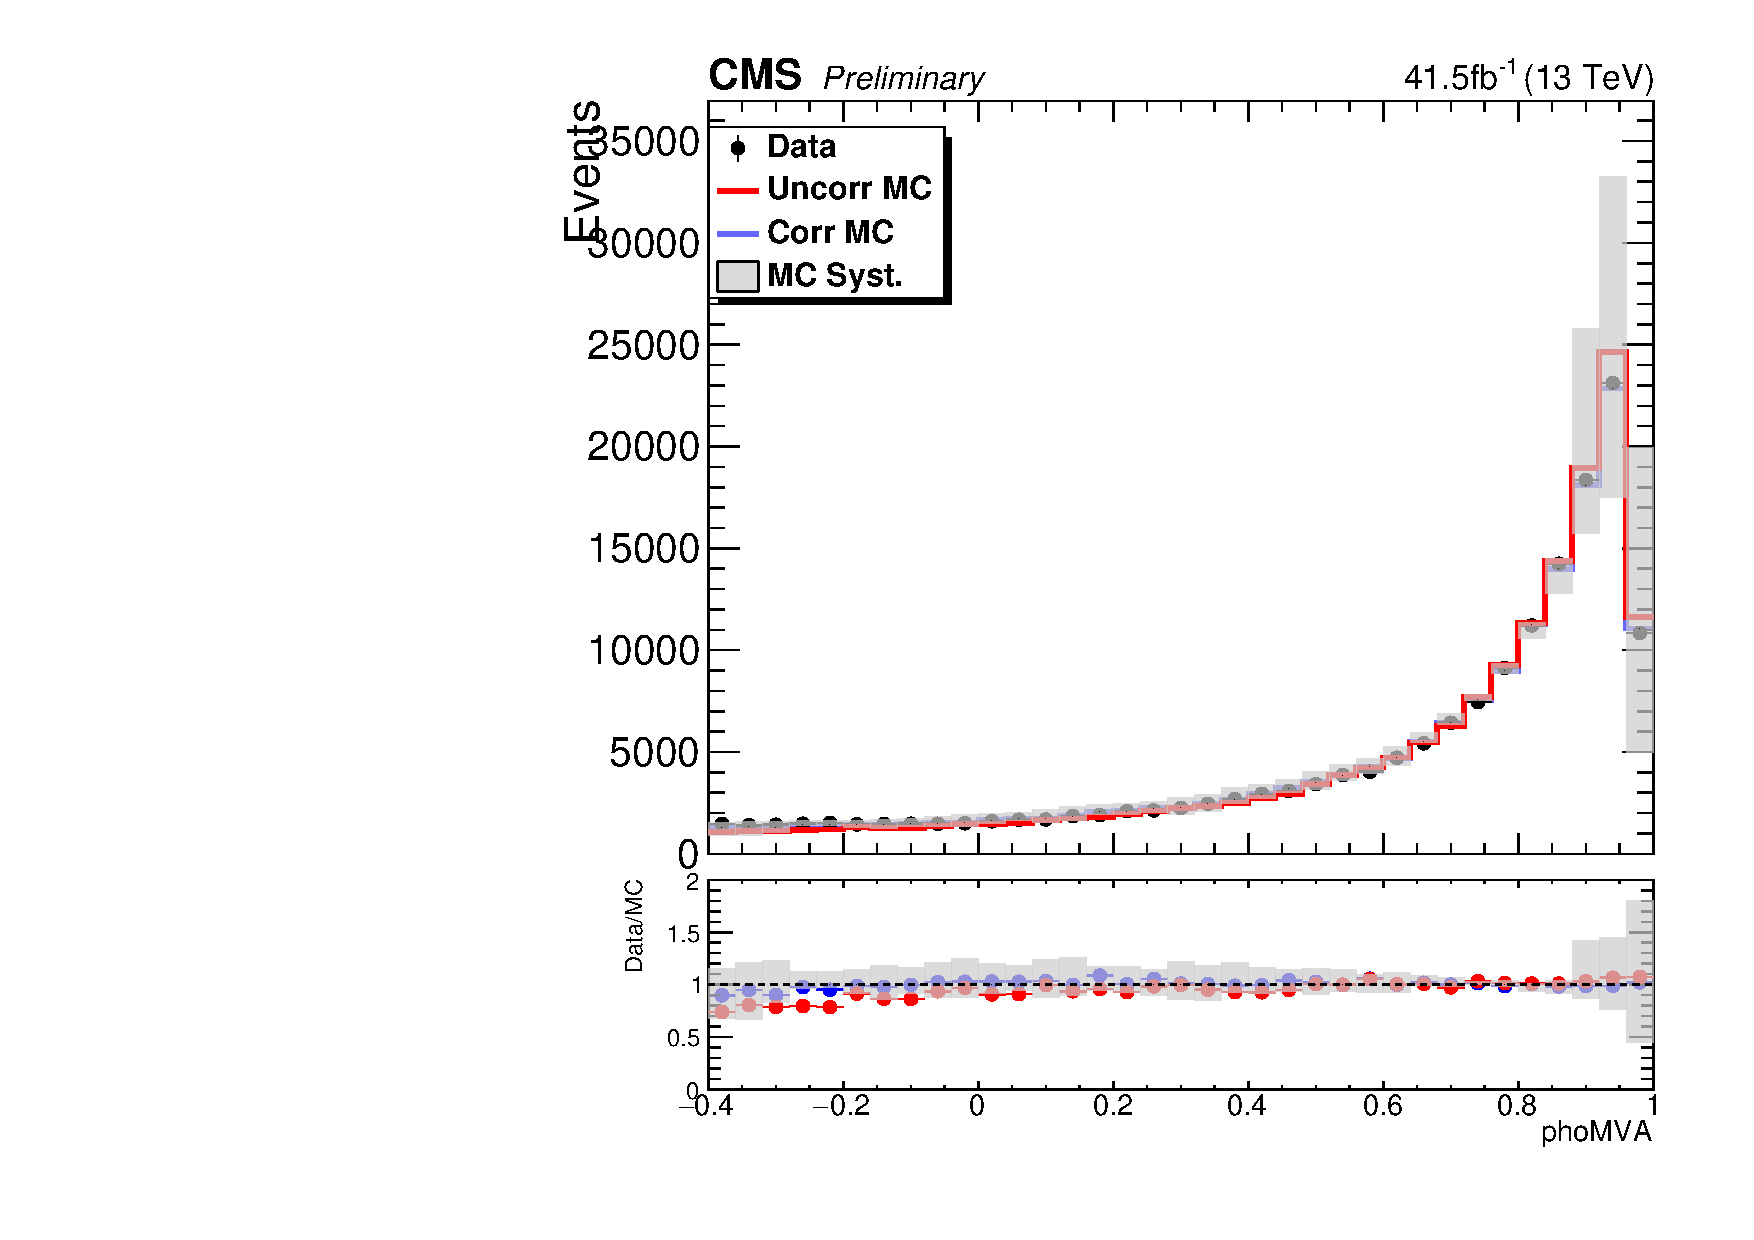
\includegraphics[width=0.35\textwidth]{fig/ss_corr/phoMVA_17_EB_Z_mmg.pdf}
		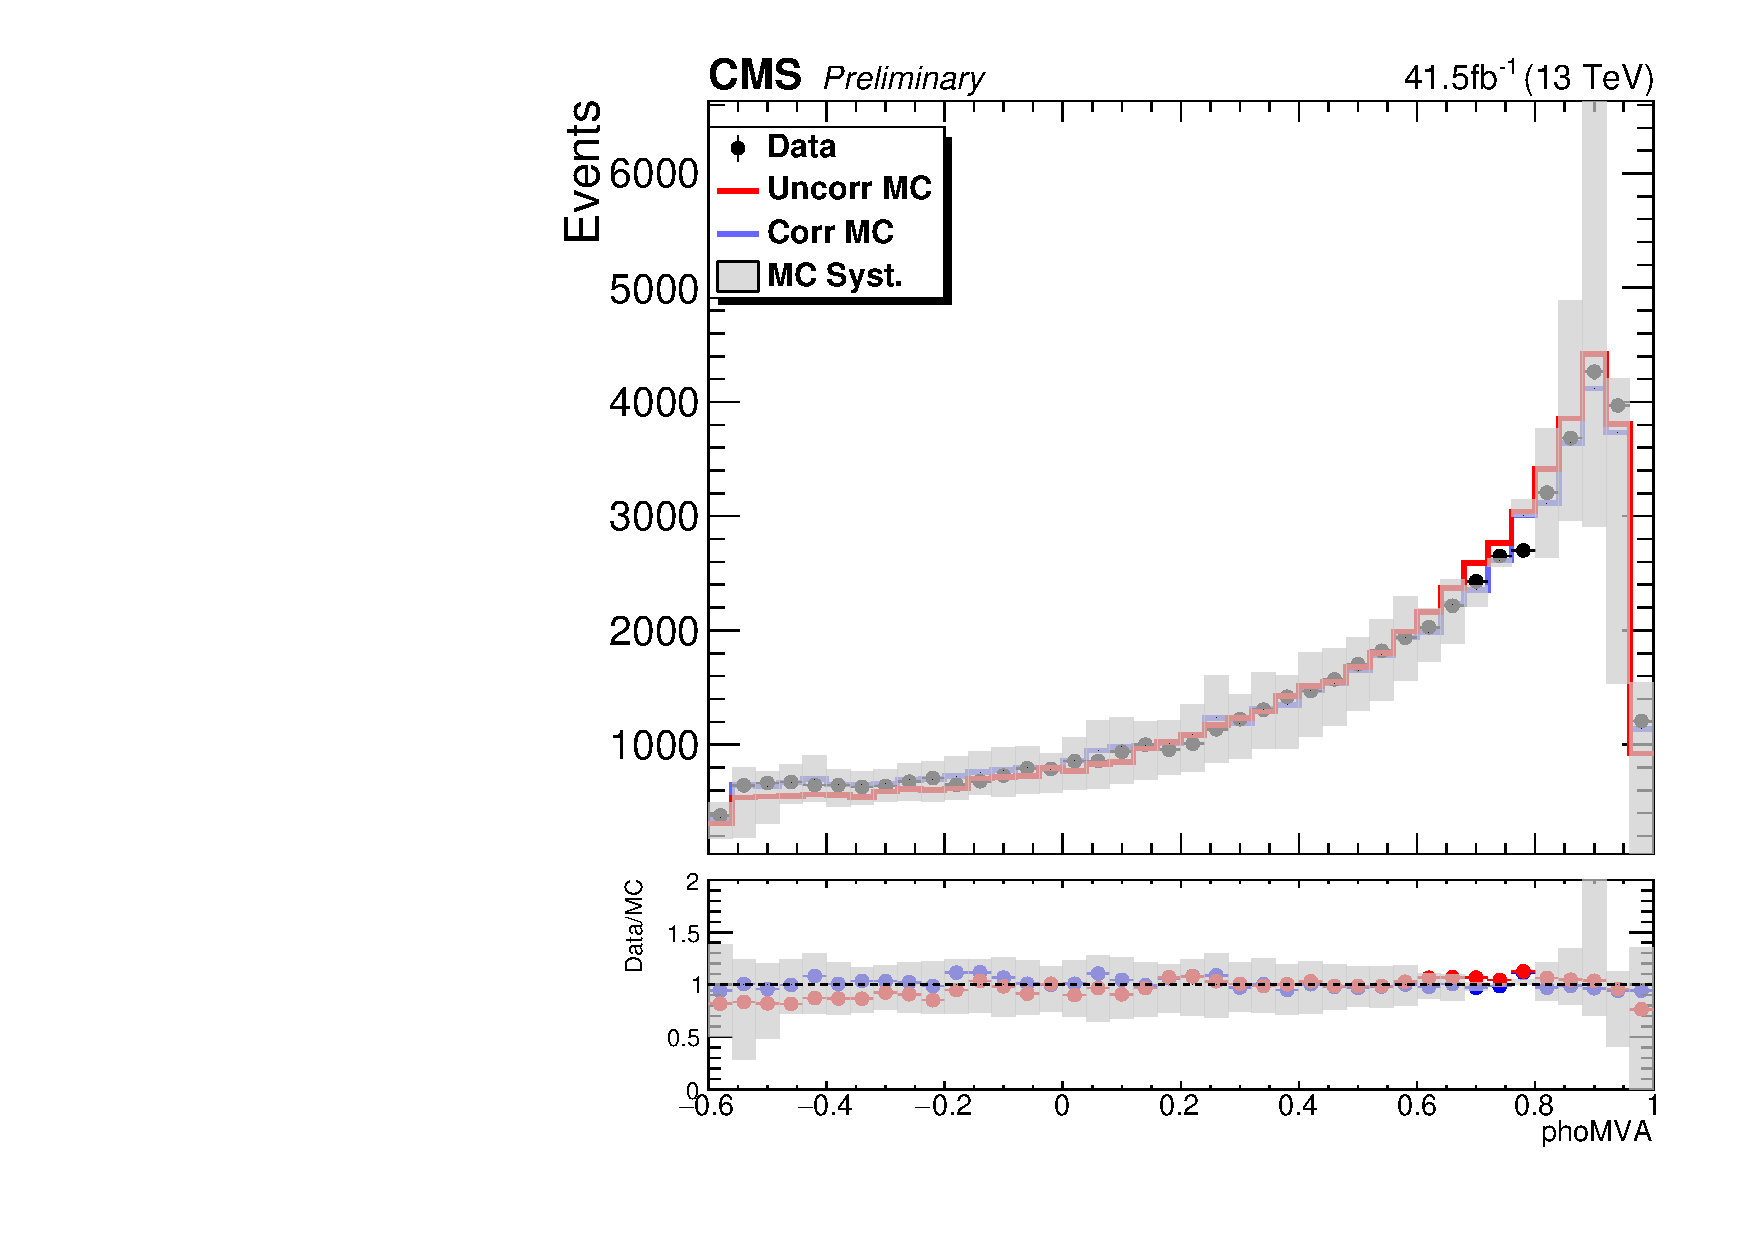
\includegraphics[width=0.35\textwidth]{fig/ss_corr/phoMVA_17_EE_Z_mmg.pdf}
	\end{center}
	\caption{Comparison of simulation with 2017 data for the photon MVA ID before and after shower shape corrections are applied to the simulation. The plots on the left (right) correspond to the barrel and endcap regions, and the upper (lower) plots correspond to $\PZ\to\epem$ ($\PZ\to\mpmm+\PGg$) events.}
	\label{fig:photon_mva_correction}
\end{figure}

Based on the corrected photon MVA ID, 90\% signal efficiency working point (WP) cuts for barrel and endcap photons 
are determined for the \hzg{} analysis. The WPs are defined based on real photons from $\Z\gamma$ simulation, and correspond 
to photon MVA ID scores greater than -0.4 (-0.59) for barrel (endcap) photons. 
These relatively loose cuts are chosen because the photon MVA ID is later used as an input to a BDT for categorization, as described in 
the next chapter.
A comparison of these WPs with the general CMS 90\% efficiency WPs, 
plotted on the receiver operator characteristic (ROC) curve for $\PZ\gamma$ (signal) and $\PZ$+jets (background)
simulation, is shown in Fig. \ref{fig:photon_mva_roc}. The efficiency of the photon MVA ID is measured with $\PZ\to\epem$ data
using a tag and probe technique. The tag electron must pass the single electron trigger with \pt threshold 27 (32) GeV in 
2016 (2017 and 2018), pass a tight cut-based identification, have \pt $>$ 30 (35) GeV for 2016 (2017 and 2018), and have $|\eta| < 2.5$. The 
probe electron must pass the corrected photon MVA ID. The corresponding SFs, measured and 
applied in bins of \pt and supercluster $\eta$, are shown in Fig. \ref{fig:photon_id_sf}. The efficiencies and SFs for the conversion-safe 
electron veto are measured by CMS using $\PZ\to\mpmm$ events with an FSR photon and are applied in the \hzg{} analysis. 
These SFs are cataloged in Table \ref{tab:eveto_sf}. 

\begin{figure}[tb]
	\begin{center}
		\includegraphics[width=0.75\textwidth]{fig/selection/photon_ID_ROC.png}
	\end{center}
	\caption{ROC curves for the corrected photon MVA ID in the barrel (red) and endcaps (blue). Here, signal refers to real photons from the $\PZ\PGg$ simulation and background refers to jets misreconstructed as photons from the $\PZ$+jets simulation. Also shown are the cuts used for the \hzg{} analysis WP and for the standard CMS 90\% WP.}
	\label{fig:photon_mva_roc}
\end{figure}

\begin{table}[tb]
	\centering   
\caption{Photon conversion-safe electron veto SFs.}
	\begin{tabular}{|c|cccccc|}

	\hline
	&\multicolumn{3}{c}{barrel} &\multicolumn{3}{c|}{endcap}\\
&0--30\GeV &30--60\GeV&60--200\GeV&0--30\GeV &30--60\GeV&60--200\GeV\\\hline
2016&\multicolumn{3}{c}{0.9938}&\multicolumn{3}{c|}{0.9875}\\
2017&\multicolumn{3}{c}{0.967}&\multicolumn{3}{c|}{0.915}\\
2018&0.987613&0.98895& 1.00006&0.95461&0.962451&0.99791\\\hline
	\end{tabular}
\label{tab:eveto_sf}
\end{table}

\begin{figure}[tb]
	\begin{center}
		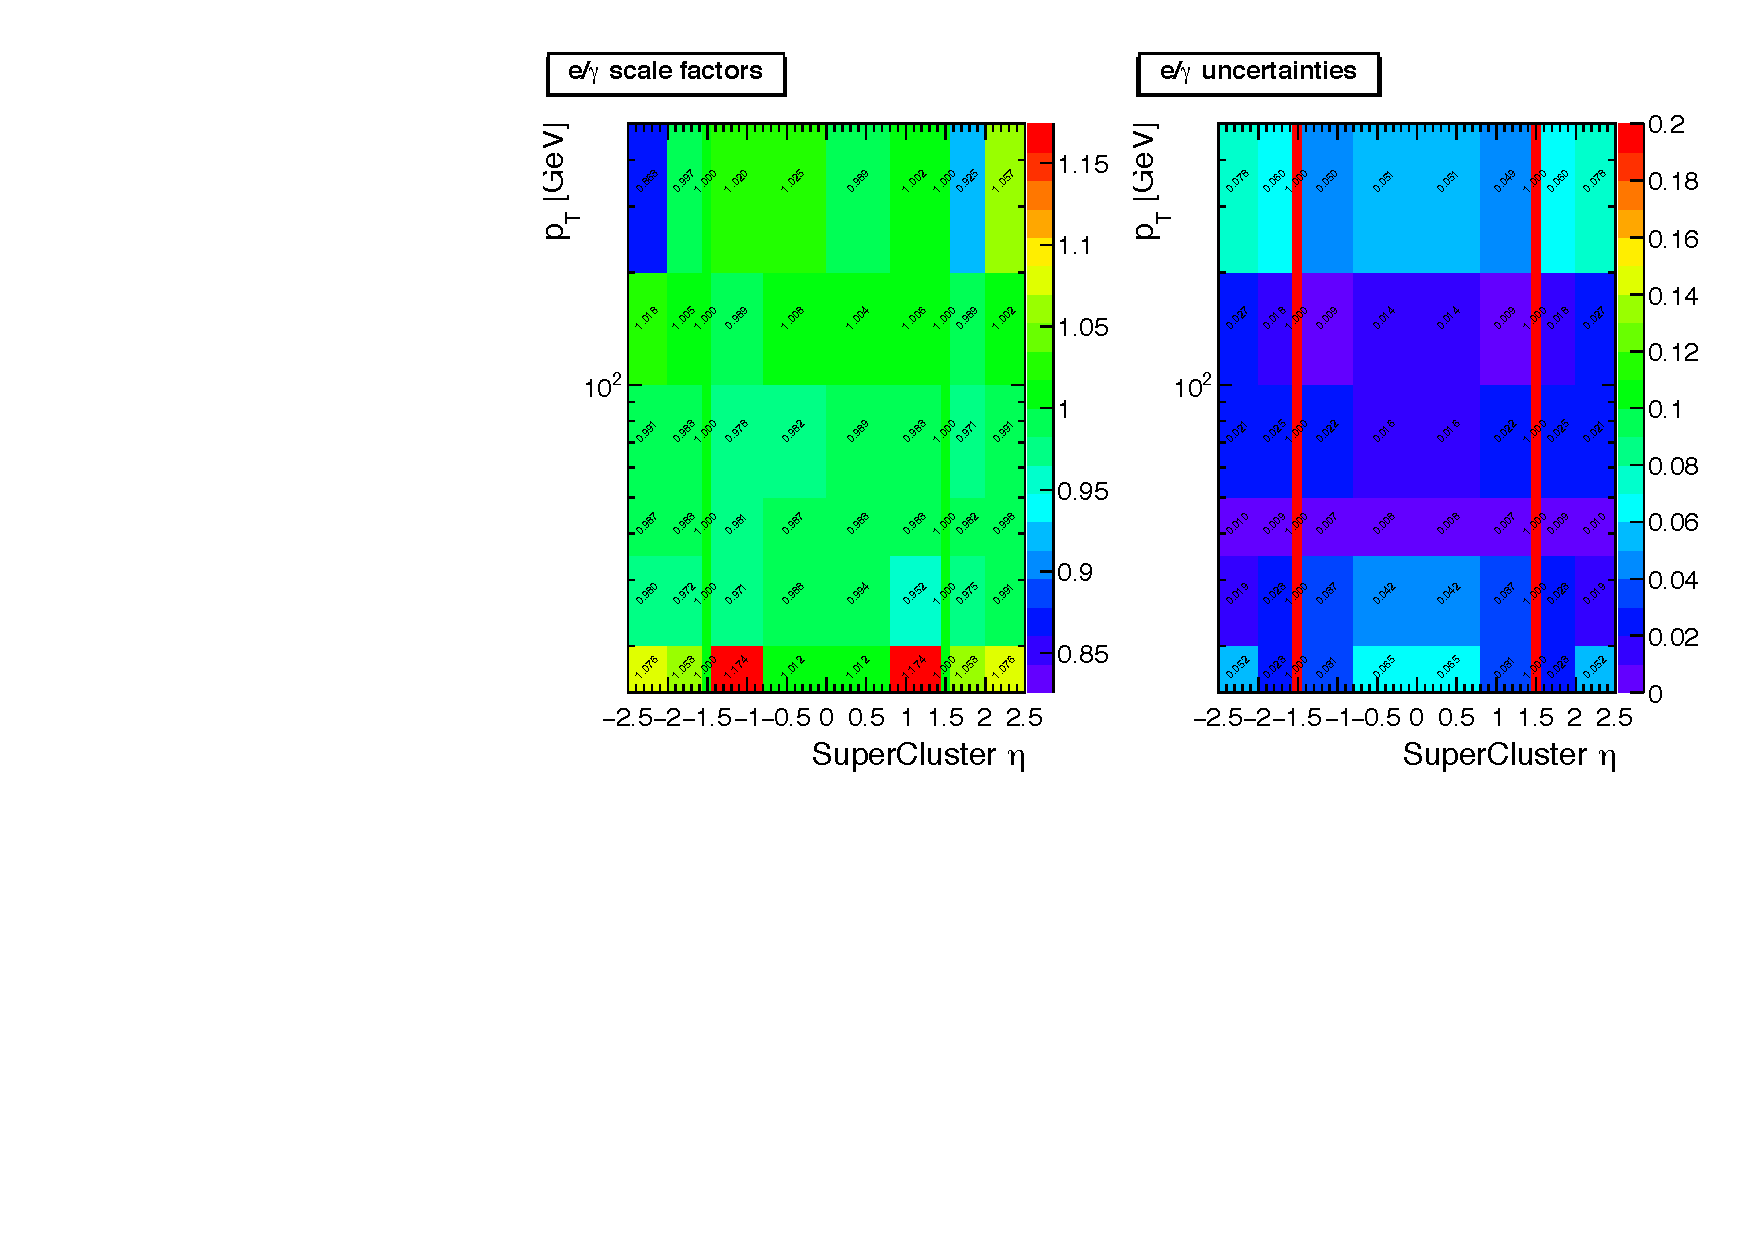
\includegraphics[width=0.6\textwidth]{fig/SFs/2016_ID_pho_2D.pdf}
		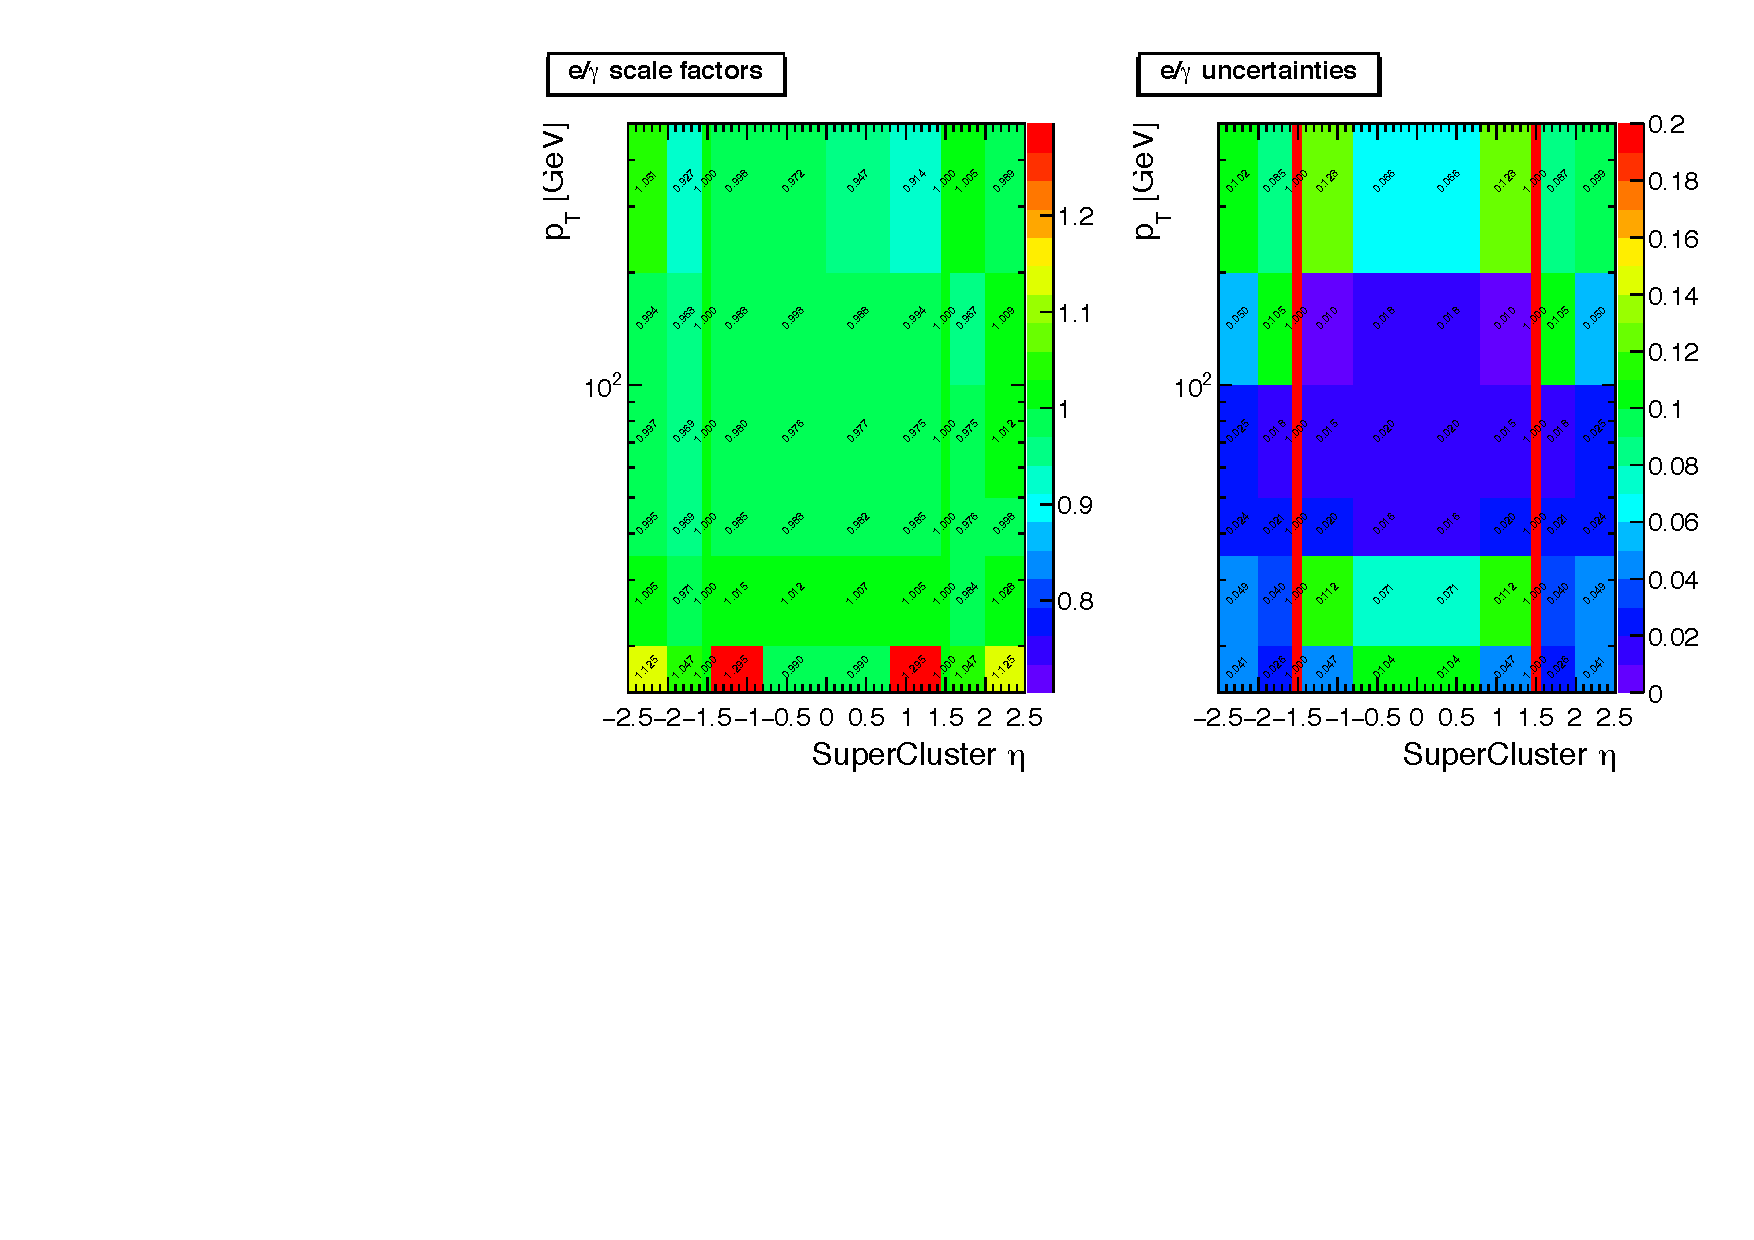
\includegraphics[width=0.6\textwidth]{fig/SFs/2017_ID_pho_2D.pdf}
		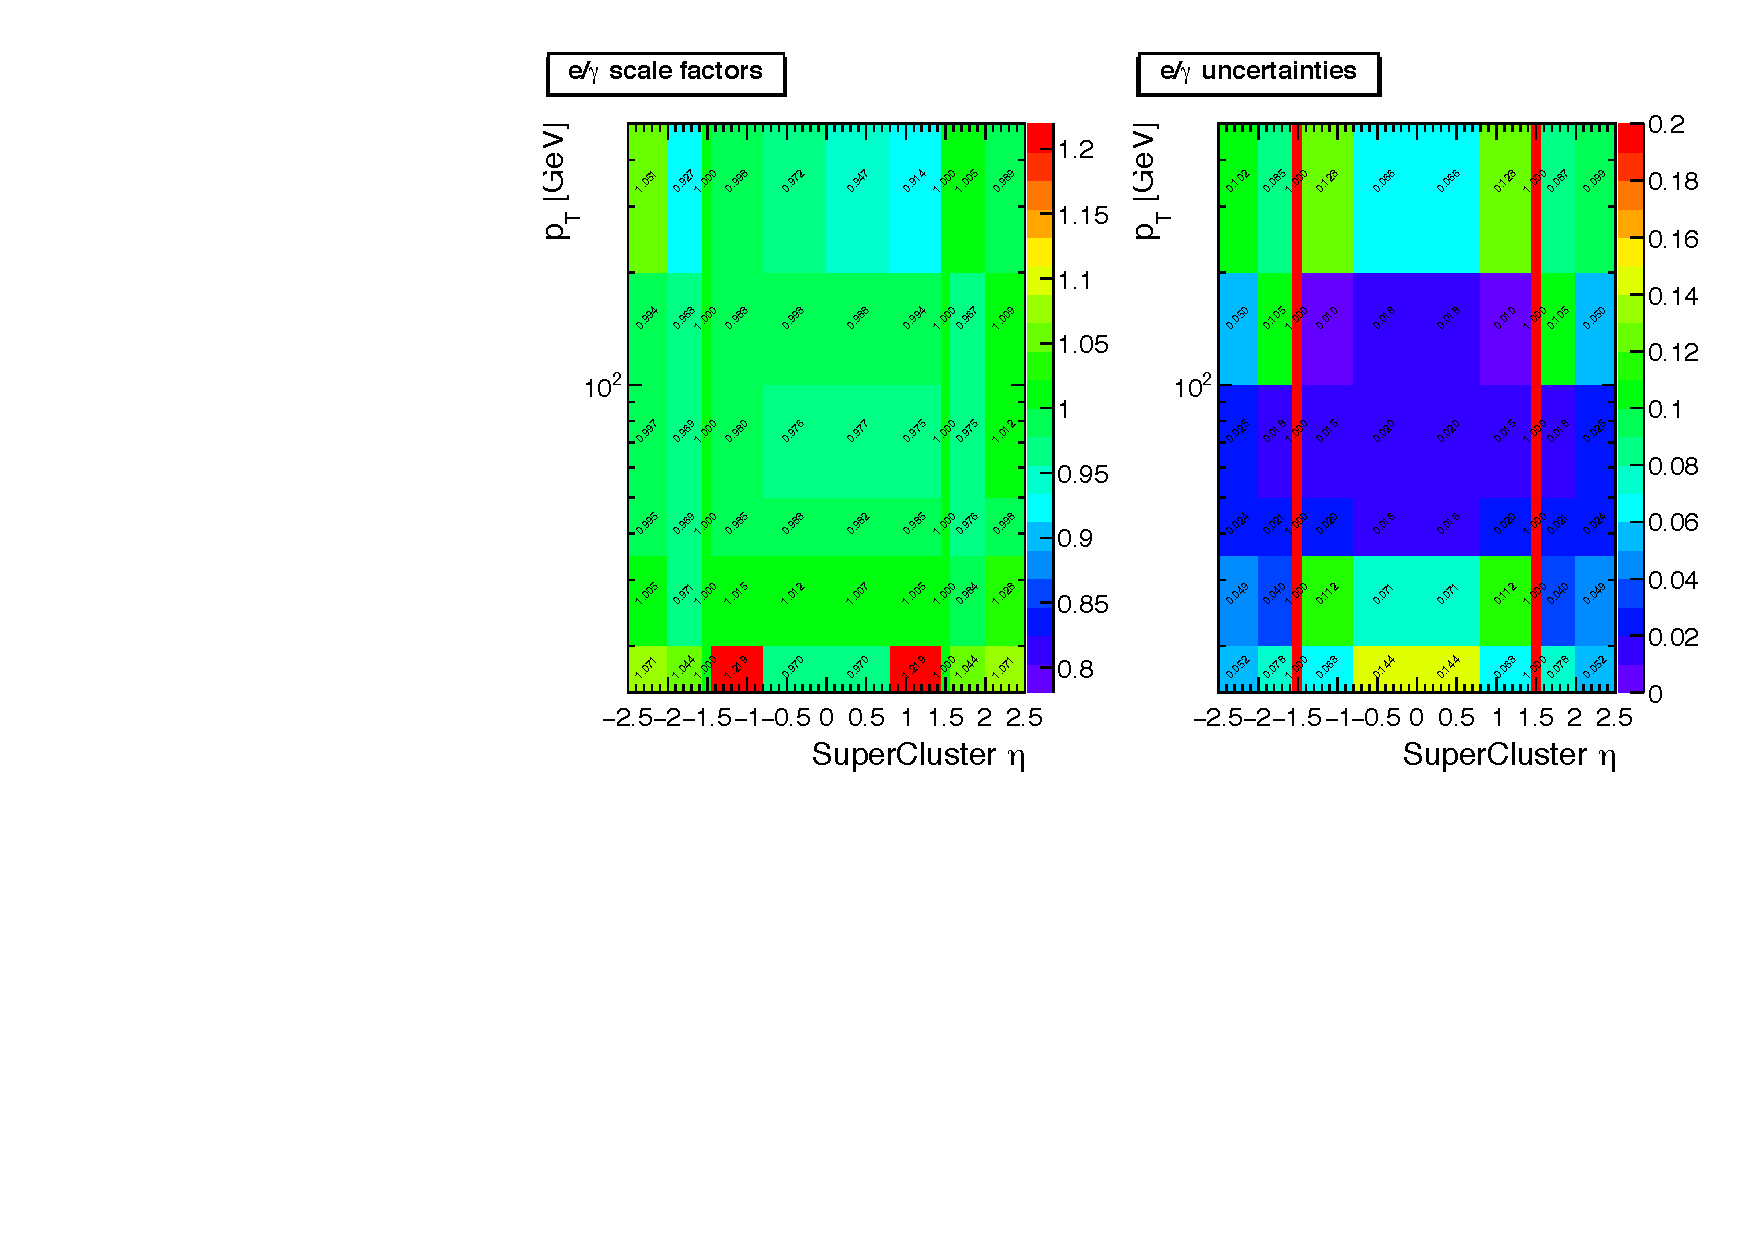
\includegraphics[width=0.6\textwidth]{fig/SFs/2018_ID_pho_2D.pdf}
	\end{center}
	\caption{Left: Photon MVA ID efficiency SFs for 2016 (upper), 2017 (middle), and 2018 (lower). Right: The corresponding uncertainties for the SFs.}
	\label{fig:photon_id_sf}
\end{figure}


\clearpage

\section{Electron Selection}
Electrons are identified using a BDT discriminant (electron MVA ID) trained on Drell--Yan plus jets simulation, 
with prompt electrons matched to generator-level objects as signal and unmatched and non-prompt electrons as background. The features 
used in the BDT training include \pt, supercluster $\eta$, shower shape variables, ratio of hadronic to electromagnetic energy, track and 
pixel hit variables, and isolation variables~\cite{EGM:ElectronID}. 
Since isolation features are included in the training of the photon MVA ID, there is no need for a separate isolation requirement. 
For the \hzg{} analysis, an electron is selected if its photon MVA ID score is higher than a loose WP
value, corresponding to 98\% signal efficiency. In addition to the photon MVA ID cut, electrons must satisfy the impact parameter requirements $|d_{xy}| < 0.5$ cm and $|d_{z}| < 1$ cm
with respect to the PV. 

Electron MVA ID efficiencies and SFs are measured using a tag and probe method on dielectron events near the 
$\PZ$ boson mass peak. The electrons used by this procedure are required to pass the single electron trigger with a \pt threshold of 27 (32) GeV for 2016 (2017 and 2018) data. 
The dielectron mass must be in the range 60--120\GeV. The tag electron must pass a tight cut-based electron ID and have 
$\pt>30\,(35)\GeV$ for 2016 (2017 and 2018) and $|\eta|<2.5$. The probe electron is required to pass the loose electron MVA ID cut and the
impact parameter cuts described above. Identification efficiencies and SFs are measured and applied in bins of 
\pt and supercluster $\eta$. The SFs for each data-taking year are shown in Fig. \ref{fig:electron_id_sf}.

\begin{figure}[tb]
	\begin{center}
		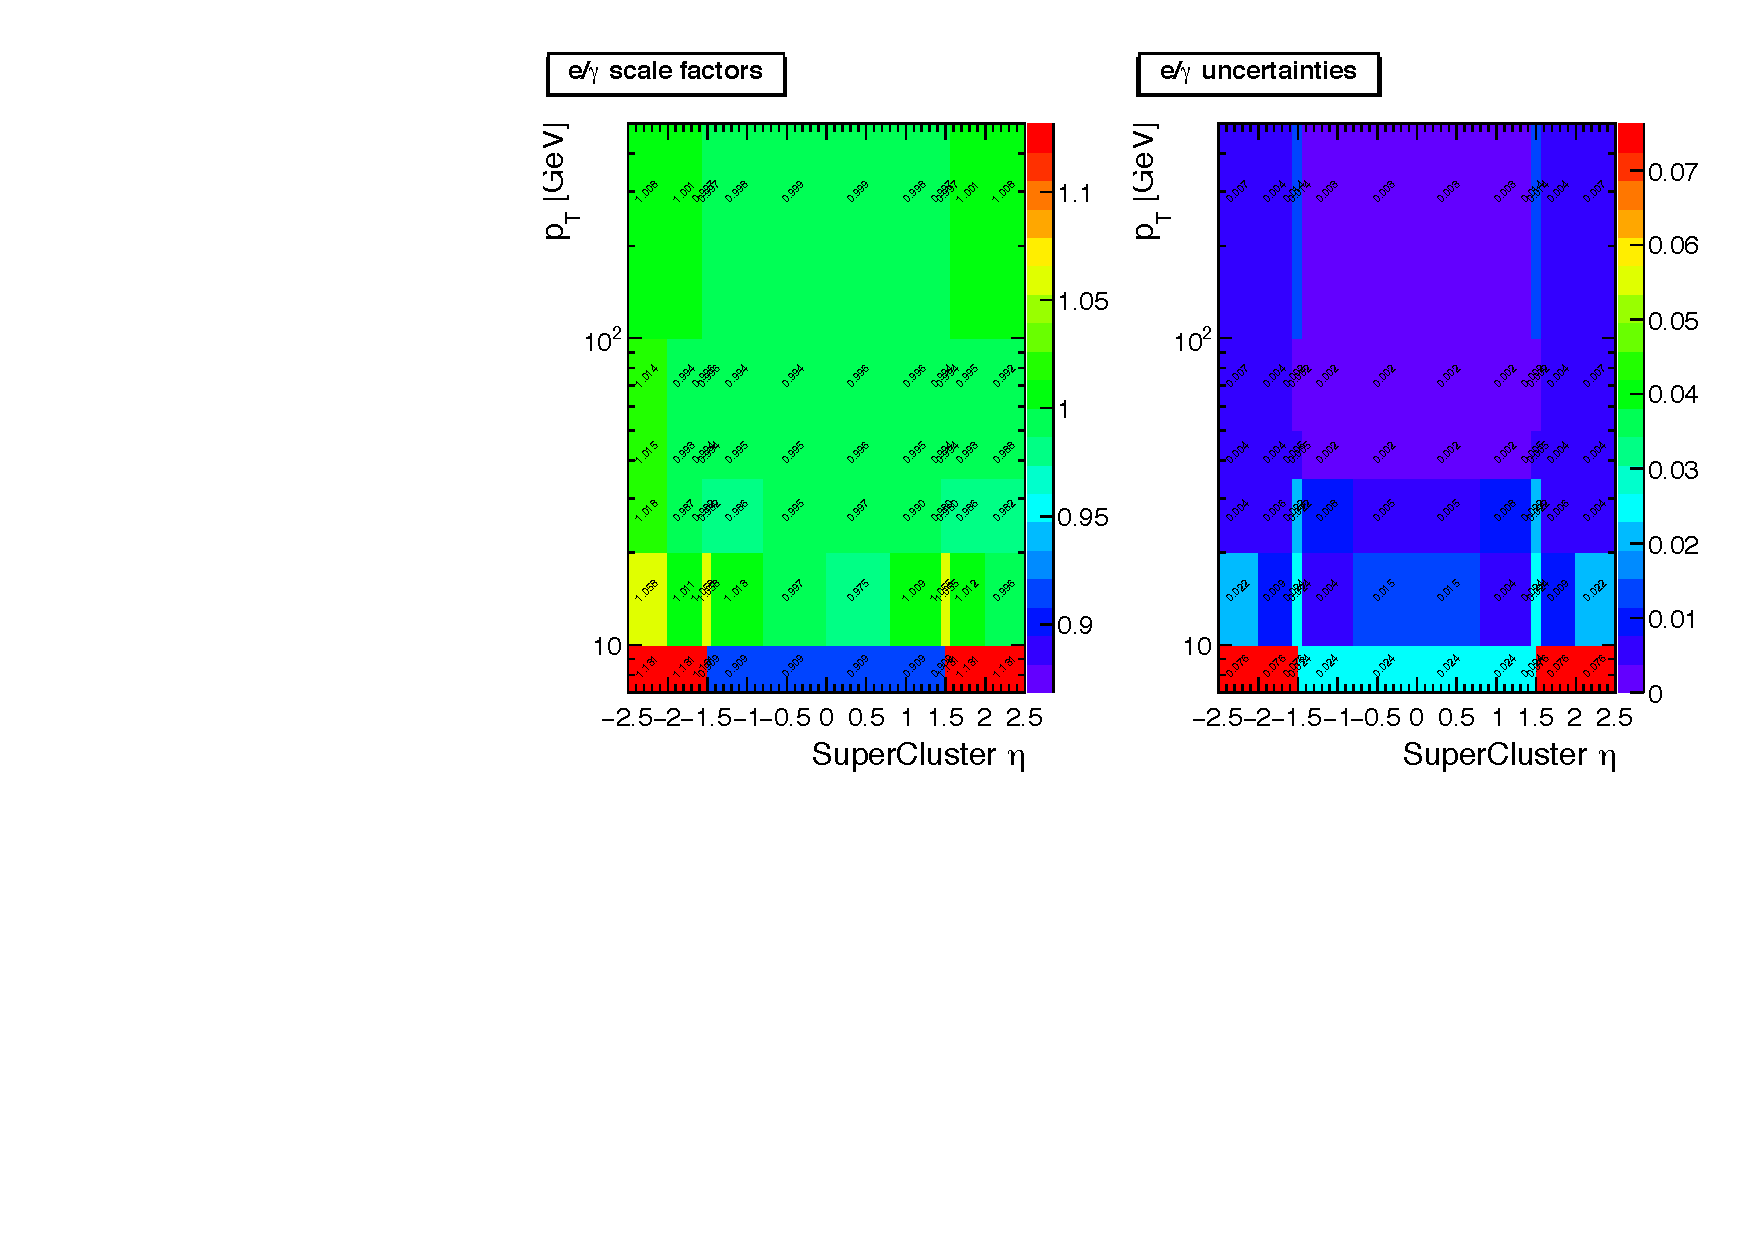
\includegraphics[width=0.6\textwidth]{fig/SFs/2016_ID_ele_2D.pdf}
		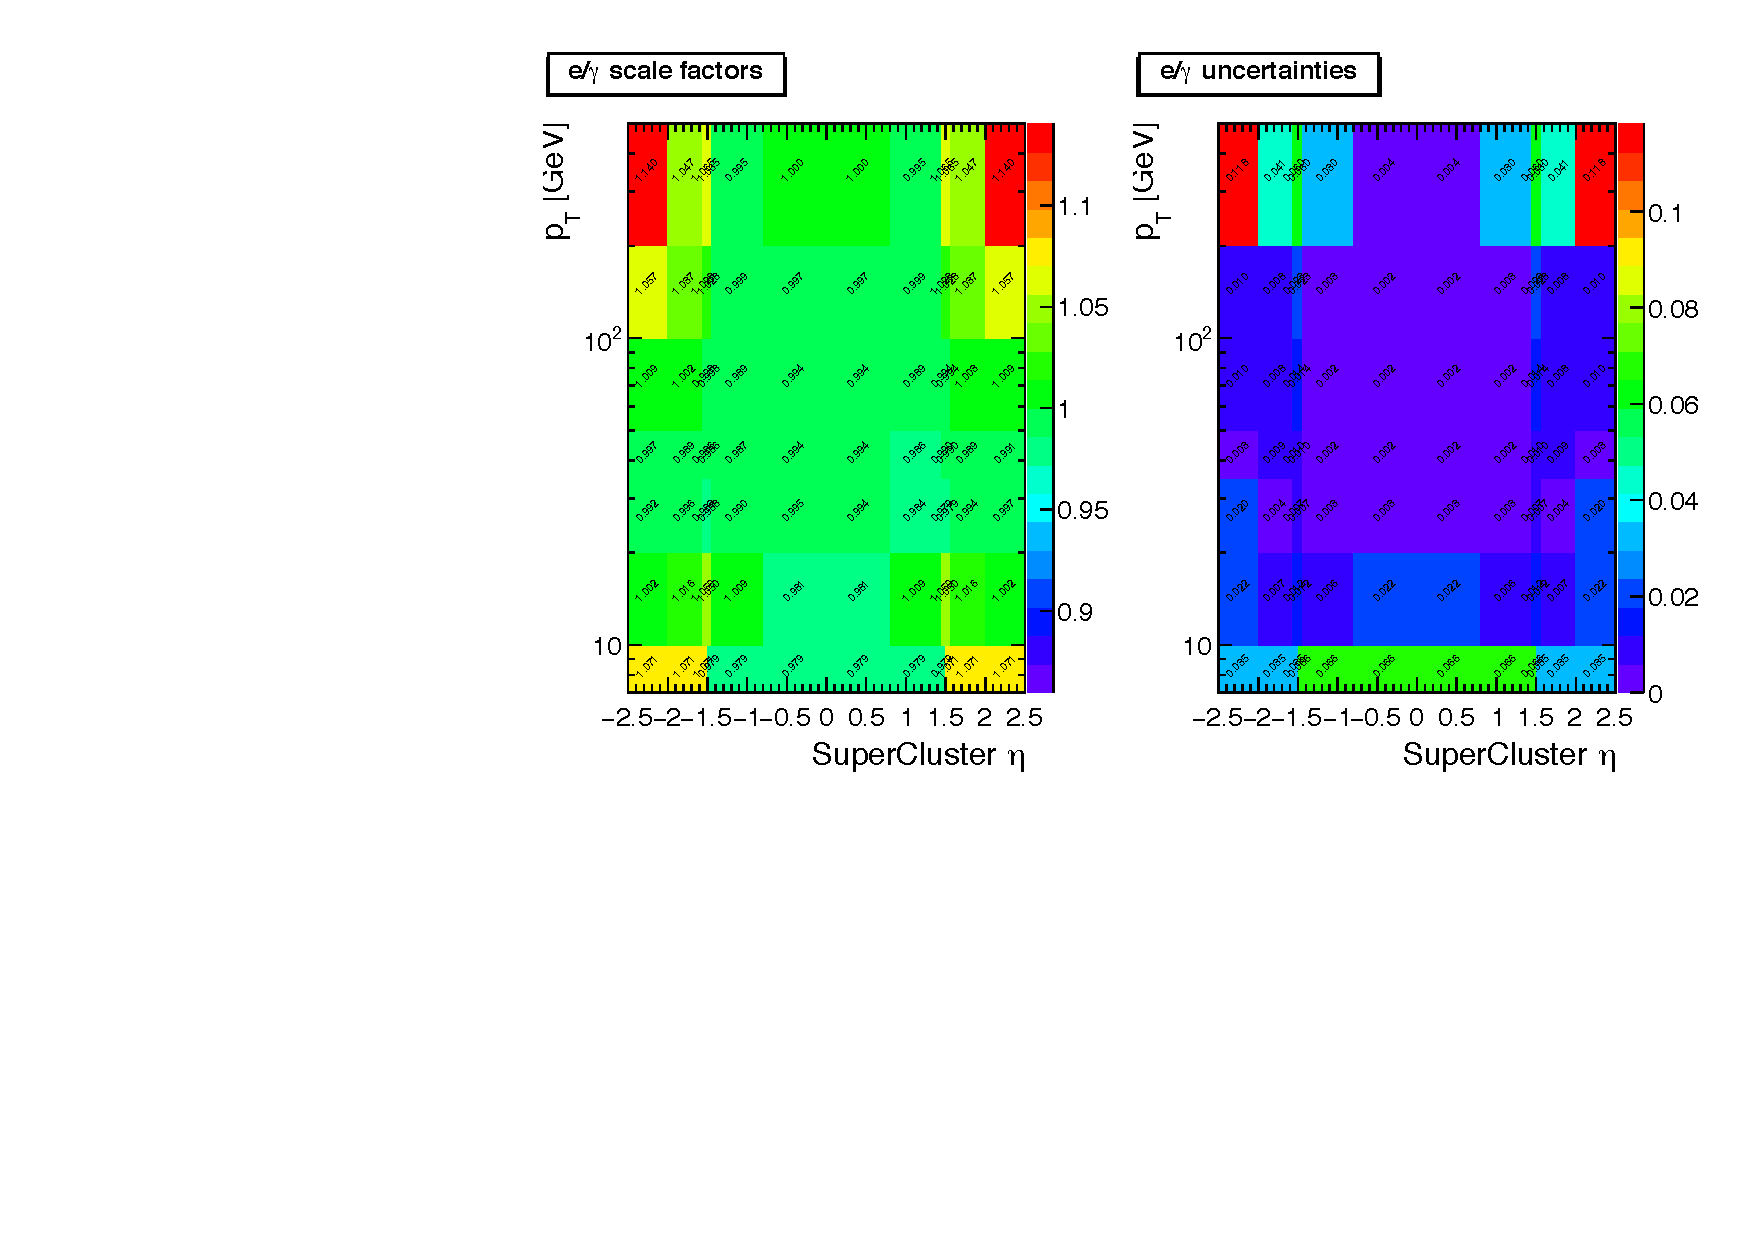
\includegraphics[width=0.6\textwidth]{fig/SFs/2017_ID_ele_2D.pdf}
		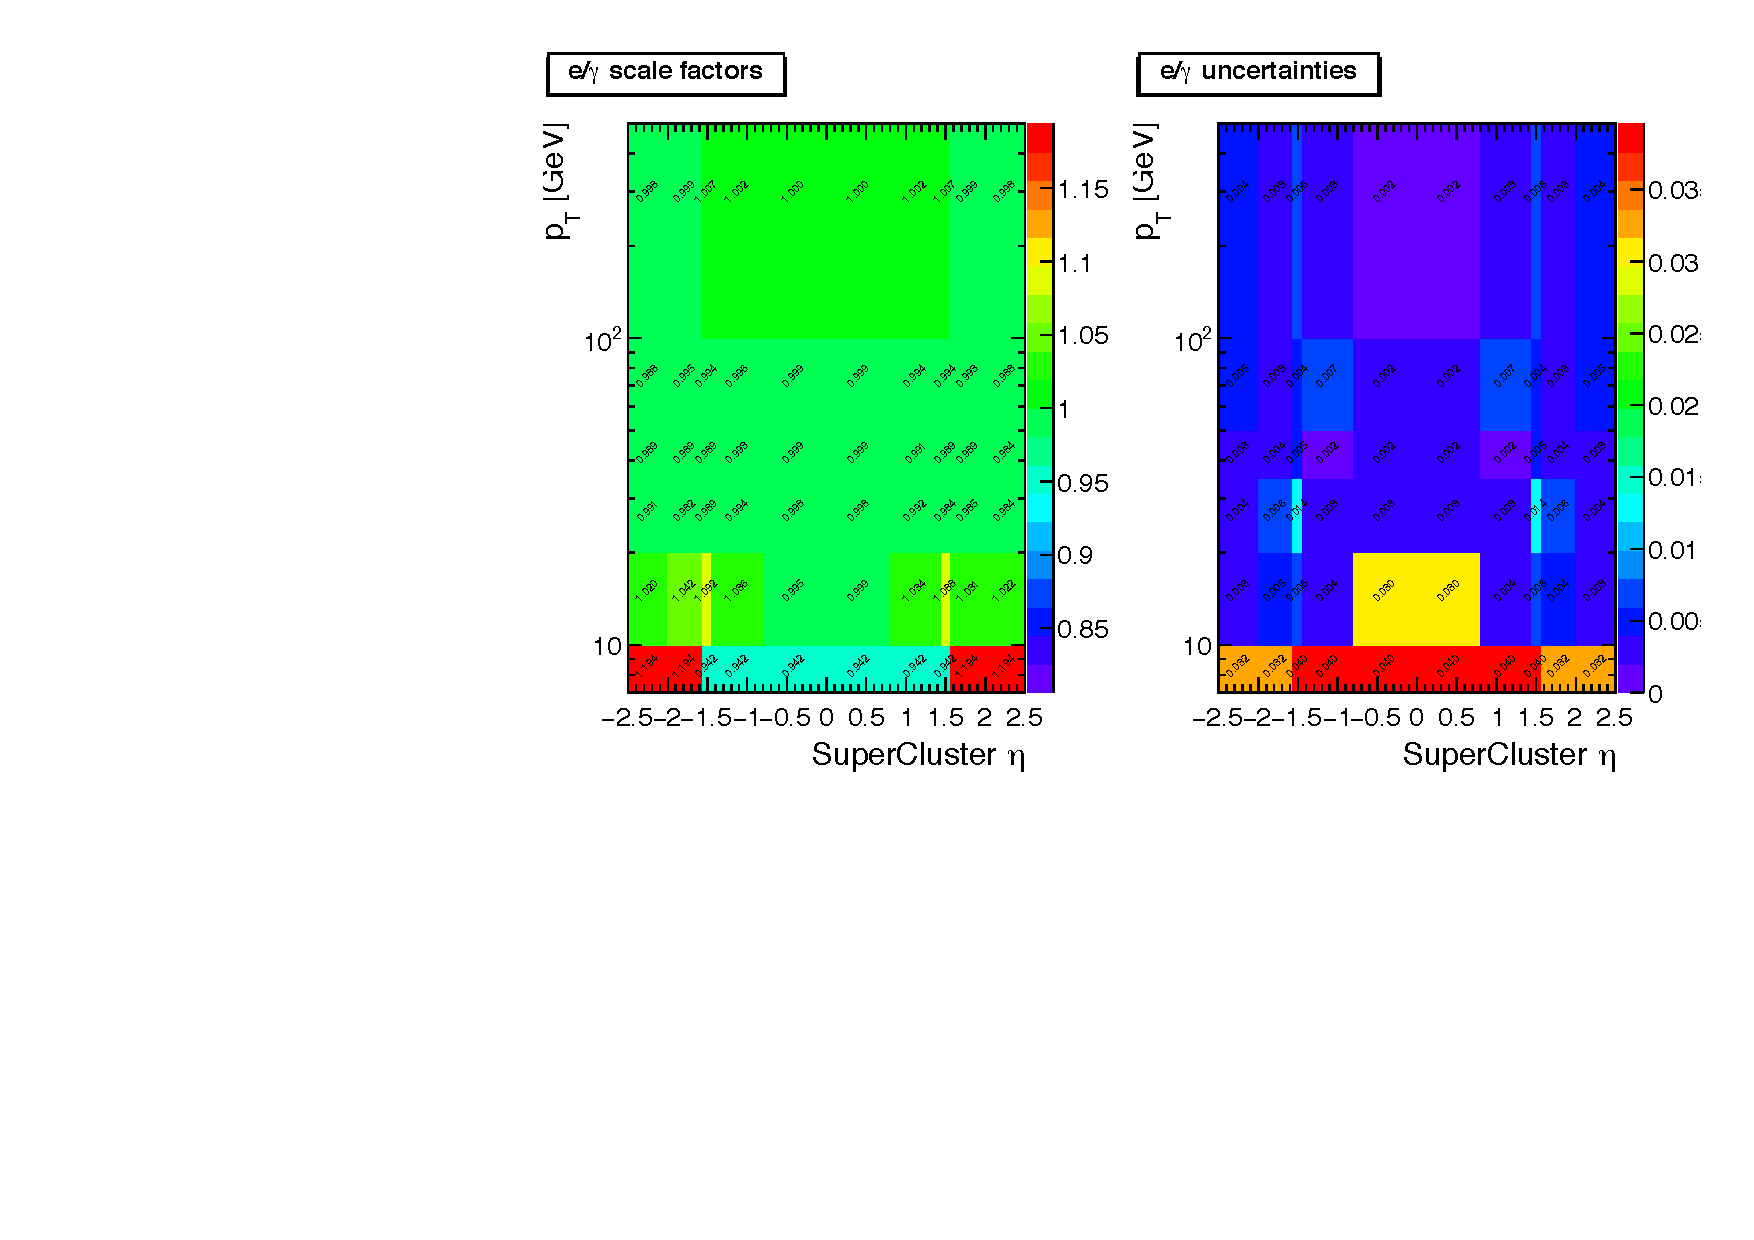
\includegraphics[width=0.6\textwidth]{fig/SFs/2018_ID_ele_2D.pdf}
	\end{center}
	\caption{Left: Electron MVA ID efficiency SFs for 2016 (upper), 2017 (middle), and 2018 (lower). Right: The corresponding uncertainties for the SFs.}
	\label{fig:electron_id_sf}
\end{figure}

\clearpage

\section{Muon Selection}
A loose cut-based muon identification is used in this analysis. This ID was originally developed for the CMS $\PH\to\PZ\PZ^*\to4\ell$ analysis of the 2016 data set~\cite{bib:htozz2016} and is well-suited for \hzg{} due to the similar kinematics of the multiple muons in the final state. 
All muons are first required to pass a set of common ID cuts, followed by a separate set of cuts for high ($>200\GeV$)
and low \pt muons. All muons are required to satisfy $|\eta| < 2.4$, $|d_{xy}| < 0.5$ \cm, and $|d_{z}| < 1$ \cm, where
the impact parameters are defined with respect to the PV using the best fit muon track. 
Additionally, the three-dimensional impact parameter with respect to the PV must have a magnitude less than four times its uncertainty.
Muons are required to either be reconstructed as global muons or tracker muons. Those with standalone tracks only in the muon system are
rejected. 
Low \pt muons satisfying the common requirements of the PF ID algorithm are selected. 
High \pt muons are selected if they pass the PF ID or if they pass
the following high \pt requirements: the muon is matched to segments in at least two muon 
stations; satisfies $\frac{p_{T}}{\sigma_{p_{T}}} < 0.3$, $|d_{xy}| < 0.2$ cm, $|d_{z}| < 0.5$ cm; has at least one pixel hit; and has
tracker hits in at least six tracker layers.

A relative PF isolation requirement is imposed, defined by the variable
\begin{equation}
\label{eqn:pfiso}
	\mathcal{I}^{\mu} \equiv \Big[ \sum \pt^\text{charged} +
                                 \max\big( 0, \sum \pt^\text{neutral}
                                 +
                                  \sum \pt^{\Pgg}
                                 - \pt^{\mu\mathrm{,PU}} \big) \Big]
                                 / \pt^{\mu}.
\end{equation}
The quantity $\sum \pt^\text{charged}$ is the scalar sum of the \pt
of charged hadrons originating from the PV,
and $\sum \pt^\text{neutral}$ and $\sum \pt^{\Pgg}$ are the scalar sums of the \pt of neutral hadrons and photons, respectively. 
The sums are over all PF candidates within a cone of radius $\DR = 0.3$ around the photon or lepton direction at the PV. 
Muons are required to satisfy $\mathcal{I}^{\mu} < 0.35$. 
The ID and isolation efficiencies and SFs with uncertainties were measured and provided by the CMS $\PH\to\PZ\PZ^*\to4\ell$ analysis working group.

In 2016, data-taking was affected by a problem in which the L1 trigger sent only one candidate per 60$^{\circ}$ sector instead 
of up to three~\cite{twiki:l1emtf}. As a result, when two muons in the same endcap had a low $\Delta \phi$ separation, only one would fire the 
trigger. To account for this, 2016 data events containing identified muons with $\Delta \phi < 70^{\circ}$ in the same endcap region 
are rejected. 


\section{Jet Selection}
Jets are selected in order to categorize events coming from potential VBF Higgs production, but no jet multiplicity requirement is present 
for the \hzg selection. In fact, the majority of simulation and data events selected in the analysis have no jets. However, identifying 
and selecting jets to categorize VBF events can still significantly improve the sensitivity of the search. Jets are required to pass 
a loose cut-based identification in 2016 and a tight cut-based identification in 2017 and 2018. These sets of identification cuts are
determined and provided by the JetMET POG. Additionally, jets must satisfy \pt $>$ 30 GeV, $|\eta| < 4.7$, and $\Delta R > 0.4$ with 
respect to each lepton and the photon selected in the analysis. An issue with noise in the ECAL endcap in 2017 caused an artificial 
increase in jet multiplicity in data within a specific kinematic phase space [REF]. To mitigate this, jets are rejected if they have 
raw \pt $<$ 50 GeV and $2.65 < |\eta| < 3.139$. This cut reduces the efficiency to reconstruct dijet pairs by 12\% in the specified 
region. To tag VBF events, we are interested in dijet pairs. To this end, if there are more than two jets satisfying the above criteria, 
only the two jets with highest \pt are selected. 

\section{Object Corrections}
Several standard corrections are applied to the physics objects selected in the analysis. Rochester muon momentum scale and resolution 
corrections are applied to both data and simulation [REF]. Energy and momentum scale and resolution corrections for electrons 
and photons are provided by the EGamma POG and applied in the analysis. Jet momentum scale and resolution correctors are provided by 
the JetMET POG and applied in the analysis. 

An additional muon momentum correction is obtained using an FSR photon recovery procedure, and is based on the procedure used by the \hzz 
analysis [REF]. FSR photons are not considered during the standard CMS muon reconstruction. As the \pt of FSR photons from radiating 
muons is generally very low, particle flow photons are considered, in contrast with the fully reconstructed photons used in the main 
analysis selection. A particle flow photon must pass a set of cuts in order to be identified as an FSR photon associated with one of the 
muons selected by the analysis. The photon must have \pt $>$ 2 GeV, $|\eta|<2.4$, and relative particle flow isolation less than 1.8. 
It must also satisfy $\Delta R(\gamma, \mu)/p_{T,\gamma}^{2} < 0.012$ and $\Delta R(\gamma, \mu) < 0.4$. If multiple particle flow 
photons pass these requirements, the photon with the smallest $\Delta R(\gamma, \mu)/p_{T,\gamma}^{2} < 0.012$ is chosen. 
Then, the four momentum of the FSR photon is added back to the four momentum of the muon, and the muon kinematics reevaluated. 
In simulation, we find that the selected FSR photon matches the generator level FSR photon with 93\% efficiency. 
Figure [FIG] shows the dilepton and three body 
invariant mass among FSR photon-containing signal events with and without applying the FSR recovery correction.
The procedure yields a 1\% improvement on the three body mass resolution in the muon channel.

\section{Event Selection}
Events are required to have at least one good primary vertex
with a reconstructed longitudinal position within 24\,{cm} of the
geometric center of the detector and a transverse position within
2\,{cm} of the nominal beam collision point. The vertex with the largest value of summed physics-object
$p_{T}^2$ is taken to be the primary interaction vertex. The physics objects used in this calculation are derived from 
information obtained from the charged-particle tracking detectors only. These objects include jets reconstructed by 
clustering charged particle tracks; the associated missing transverse momentum, defined as the negative vector sum of the \pt of 
those jets.

Events with two same-flavor opposite sign leptons (e or $\mu$) and a photon are selected. The leading muon (electron) is required to have 
\pt greater than 25 (20) GeV, and the trailing lepton must have \pt greater than 15 (10) GeV. Electrons (muons) must have $|\eta|$ 
less than 2.5 (2.4). The photon must have \pt greater than 15 GeV and must satisfy $0 < |\eta| < 1.4442$ or $1.566 < |\eta| < 2.5$. 
This avoids the calorimeter transition region, in which photon reconstruction is more difficult. The invariant mass of the dilepton 
system is required to be greater than 50 GeV. In events with multiple dilepton pairs, the pair with mass closest to the nominal 
Z boson mass [REF] is selected. 

Events are required to have a photon satisfying $p_{T}^{\gamma}/m_{\ell\ell\gamma} > 0.14$, which suppresses the Z plus jets 
background without significantly reducing signal efficiency and without significantly shaping the three body mass spectrum.
Each lepton must have $\Delta R > 0.4$ with respect to the photon. To reject events with final-state radiation from 
Drell-Yan processes, we require $m_{\ell\ell\gamma} + m_{\ell\ell} > 185$ GeV. Finally, the three body mass is required to 
satisfy $105 < m_{\ell\ell\gamma} < 170$ GeV. 

\section{Kinematic Fit}
A kinematic fit technique is used to improve the dilepton mass resolution. This constrains the dilepton mass based on the true 
Z boson lineshape while accounting for the known detector resolution. The position information of the leptons has a negligible impact
on the fit, so only the lepton transverse momenta and dilepton mass are included in the fit. The procedure is based on previous
studies by the \hzz analysis [REF]. We do not carry out an analogous kinematic fit for the $m_{\ell\ell\gamma}$ invariant 
mass in order to avoid any potential bias due to reshaping the mass distribution. The kinematic fit is a maximum likelihood fit 
defined by the likelihood function below: 

\begin{equation}
\begin{aligned}
\mathcal{L}({P_{T}}^{1},{P_{T}}^{2}|{P_{T}}^{reco1},{\sigma_{P_{T}}}^1,{P_{T}}^{reco2},{\sigma_{P_{T}}}^2) \\
=Gauss({P_{T}}^{reco1}|{P_{T}}^{1},{\sigma_{P_{T}}}^1)\cdot Gauss({P_{T}}^{reco2}|{P_{T}}^{2},{\sigma_{P_{T}}}^2)\cdot\mathcal{L}(m_{12}|m_{Z})
\end{aligned}
\end{equation}

Here, $p_{T}^{reco1}$ and $p_{T}^{reco2}$ are the reconstructed transverse momenta of the two leptons, 
$\sigma_{p_{T}}^{1}$ and $\sigma_{p_{T}}^{2}$ are the per-lepton transverse momentum resolutions, 
$p_{T}^{1}$ and $p_{T}^{2}$ are the parameters to optimize, and $m_{12}$ is the invariant mass 
calculated from $p_{T}^{1}$ and $p_{T}^{2}$. $\mathcal{L}(m_{12}|m_{Z})$ is the likelihood given the true Z mass lineshape. 
The outputs of the fit are $p_{T}^{1}$ and $p_{T}^{2}$.
Their uncertainties are saved and used to calculate a per-event uncertainty for the mass measurement.
To optimize this procedure, we determine the true generator level Z lineshape from a gluon-gluon fusion \hzg sample.
Generator level Z lineshapes for the dielectron and dimuon final states are fit with 
a single-sided Crystal Ball function plus three gaussian functions.
For each event, the likelihood is maximized and the \pt information of the refit leptons is updated. 
Then, the dilepton mass and three body mass are recalculated based on the refit leptons.
The mass distributions for before and after the kinematic fit are shown in Figure [FIG]. The level of improvement in the 
dilepton mass resolution, 
as measured by $\sigma_{eff}$, is shown in in Table \ref{tab:sig_eff_refit}.

\begin{table}[h]
    \begin{center}
    \caption{
        Percent improvement in dilepton and three-body mass resolution (measured by $\sigma_{eff}$) 
        after the kinematic fit.
      }
        \begin{tabular}{|c|cc|cc|}
      \hline
               & \multicolumn{2}{c|}{\textbf{electron channel}}   & \multicolumn{2}{c|}{\textbf{muon channel}}               \\
	  \hline
		&$m_{ee}$&$m_{ee\gamma}$&$m_{\mu\mu}$&$m_{\mu\mu\gamma}$\\\hline
            \textbf{2016} & 20\% & 20\%& 17\% &12\%\\ 
      \hline
            \textbf{2017} & 28\% & 27\%& 21\% &11\%\\ 
      \hline 
            \textbf{2018} & 24\% & 24\%& 20\% &10\% \\ 
      \hline 
    \end{tabular}
    \label{tab:sig_eff_refit}
    \end{center}
\end{table}

We also perform a closure test on the background as shown in Figure [FIG]. The dilepton mass should be constrained,
while the three body mass should not be distorted by the kinematic constraint. Indeed, this is what is observed.


\chapter{Event Categorization}\label{sec:categorization}
The sensitivity of the \hzg{} search can be significantly improved by leveraging the differences between signal events
arising from different Higgs boson production mechanisms. In general, these production mechanisms have different final state topologies and kinematics. 
Mutually exclusive categories are defined in order to take advantage of this. 
In previously published CMS searches for \hzg{}, cut-based approaches were used to define the categories. However, in the present analysis, 
the categorization strategy has been updated and improved using machine learning methods. The remainder of this chapter describes the categorization 
strategy in detail and summarizes the final categories used in the full Run 2 \hzg{} analysis.

The signal candidates from the $\mathrm{V}\PH$ and $\ttbar\PH$ production mechanisms are targeted using a lepton-tagged category, 
in which at least one electron or muon is present beyond those used to reconstruct the 
$\PZ\gamma$ system.
The signal candidates from the VBF production mechanism are targeted by identifying events that have an additional dijet system. 
A BDT classifier (referred to as the VBF BDT) uses the properties of this dijet system to divide such events 
into a set of dijet categories. The VBF BDT discriminant value, transformed such that the VBF signal distribution is uniform,
is denoted by $\DVBF$.
The signal candidates from the $\Pg\Pg\PH$ production mechanism are targeted with events that do not fall within the 
lepton-tagged or dijet categories. A BDT classifier (referred to as the kinematic BDT), trained on a set
of kinematic variables, is used to further discriminate between signal and background events,
defining a set of untagged categories. The kinematic BDT discriminant value, transformed such that the total signal 
distribution is uniform, is denoted by $\Dkin$. 

\section{Kinematic Boosted Decision Tree}
The kinematic BDT is used to distinguish \hzg{} signal events from background events based on the kinematics of the leptons and photon in the $\PZ\gamma$ candidate system, as well as on the measured properties of these physics objects.
It is trained using simulated \hzg{} signal events from all Higgs boson production modes described in Chapter \ref{sec:data} and background events from $\PZ\gamma$, $\PZ$+jets, $\ttbar$, and VBS $\PZ\gamma$. The training is restricted to use half of the simulated events, with the other half 
reserved for subsequent category optimization and signal $m_{\lplm\gamma}$ shape modeling. All training events are required to pass the object and 
event selection criteria described in Chapter 6. Events from 2016, 2017, and 2018 simulation samples in both the muon and electron channels 
are combined for training, weighted by their respective cross sections and by the recorded integrated luminosity of each data-taking year.

\subsection{Training Features}
The choice of training variables (features) for the kinematic BDT is guided by existing theoretical physics knowledge, categorization strategies in the prior \hzg{} analyses, and empirical methods. From a theoretical perspective, the decay angles between the final state particles are known to provide 
some discriminating power between signal and background. These angular features, described in Refs. \cite{HZg_angle1,HZg_angle2}, include $\cos\Theta$, $\cos\theta$, and $\phi$, where $\Theta$ is the production angle of the $\PZ$ boson in the Higgs boson center-of-mass frame, and $\theta$ and $\phi$ are the polar and azimuthal decay angles of the leptons in the $\PZ$ boson center-of-mass frame, respectively. Figure \ref{fig:kinangles} shows how these angles are defined, and Fig. \ref{fig:kin_GEN_angles} shows the theoretical and reconstructed distributions of these quantities. Based on the theoretical distributions, these angular features are expected to offer good discriminating power between signal and background. However, it must be noted that the discriminating power is reduced for the final reconstructed quantities, since these angles are highly correlated with other analysis selection requirements, such as the mass cuts. 

\begin{figure}[tb]
	\begin{center}
		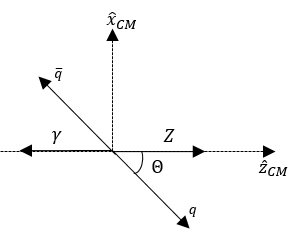
\includegraphics[width=0.3\textwidth]{fig/MVA/HZg_angle2.png}
		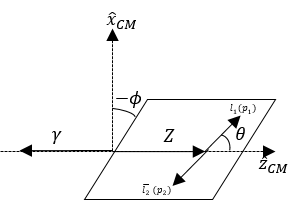
\includegraphics[width=0.3\textwidth]{fig/MVA/HZg_angle1.png}
	\end{center}
	\caption{Definitions of theoretical angles used for kinematic BDT training. The left diagram is in the Higgs boson center-of-mass frame, and the right diagram is in the $\PZ$ boson center-of-mass frame.}
	\label{fig:kinangles}
\end{figure}

\begin{figure}[tb]
	\begin{center}
		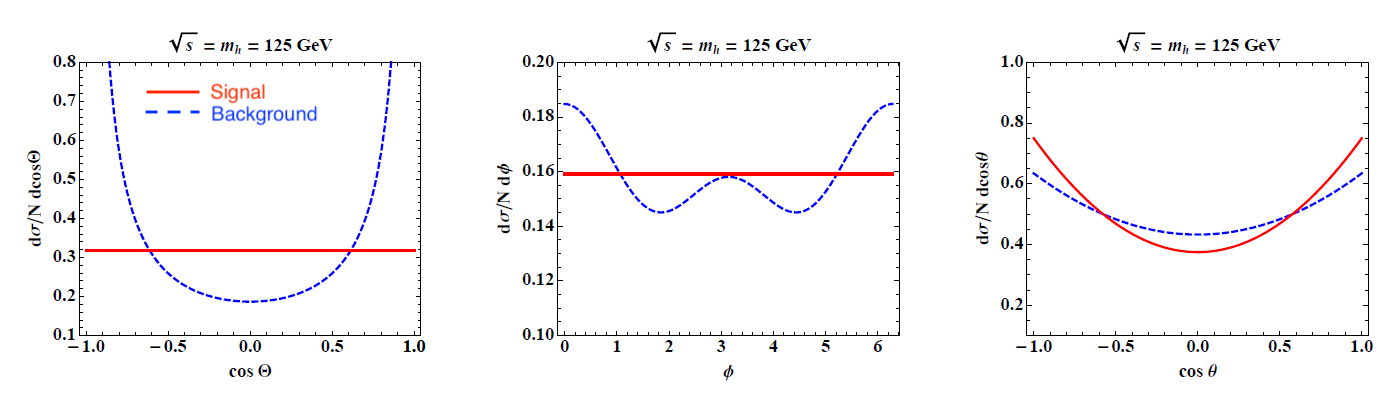
\includegraphics[width=0.9\textwidth]{fig/MVA/Zg_theorist.png}
		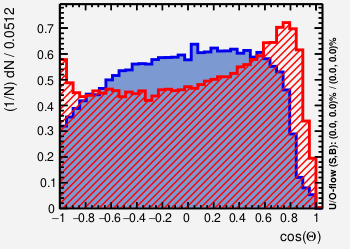
\includegraphics[width=0.3\textwidth]{fig/MVA/cosTheta_reco.png}
		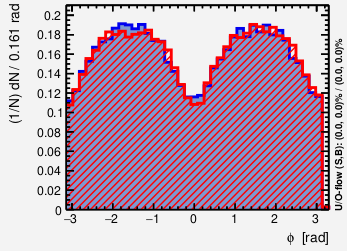
\includegraphics[width=0.3\textwidth]{fig/MVA/phi_reco.png}
		\includegraphics[width=0.3\textwidth]{fig/MVA/costheta_reco.png}
	\end{center}
	\caption[Top: Expected theoretical shapees for the angular features used for kinematic BDT training. Bottom: Reconstructed shapes for these quantities after the \hzg{} selection requirements have been applied. Please note that the red and blue color conventions are reversed for the top and bottom plots.]
	{Top: Expected theoretical shapes~\cite{HZg_angle1} for the angular features used for kinematic BDT training. Bottom: Reconstructed shapes for these quantities after the \hzg{} selection requirements have been applied. Please note that the red and blue color conventions are reversed for the top and bottom plots.} \label{fig:kin_GEN_angles}
\end{figure}

Several fundamental kinematic quantities of the final state particles are also used as training features. These include the pseudorapidity of each lepton, the $\Delta R$ between each lepton and the photon, and the $\pt/m$ of the $\lplm\gamma$ system. We note that the \pt values of each final state particle were also considered for training, but were found to have a negligible impact on discrimination power. This is likely because they are highly correlated with these other fundamental kinematic quantities, and thus, do not introduce much additional information to the BDT model. A comparison between signal and background shapes for these kinematic features is shown in Fig. \ref{fig:kin_training_shapes}.

\begin{figure}[tb]
	\begin{center}
		\includegraphics[width=0.3\textwidth]{fig/MVA/lepeta1_reco.png}
		\includegraphics[width=0.3\textwidth]{fig/MVA/lepeta2_reco.png}
		\includegraphics[width=0.3\textwidth]{fig/MVA/phoeta_reco.png}
		\includegraphics[width=0.3\textwidth]{fig/MVA/mindr_reco.png}
		\includegraphics[width=0.3\textwidth]{fig/MVA/maxdr_reco.png}
		\includegraphics[width=0.3\textwidth]{fig/MVA/pt_over_m_reco.png}
	\end{center}
	\caption{Comparison of reconstructed signal and background shapes for several kinematic variables used for kinematic BDT training. The blue histograms represent the signal, while the red histograms represent the background.}
	\label{fig:kin_training_shapes}
\end{figure}

Finally, training features related to the quality of the final state photon are used. These include the corrected photon MVA ID score and the photon energy resolution. There are several motivations for these features. First, they are important for distinguishing \hzg{} signal events from the large $\PZ$+jets background, where a jet is misreconstructed as a photon. Second, they are inspired by the previous CMS \hzg{} searches, which used photon pseudorapidity and $R_{9}$ for categorization. In our current analysis, the photon $R_{9}$ was also considered as a training feature. However, it did not contribute any meaningful additional discriminating power. This is likely because the $R_9$ is already part of the corrected photon MVA ID. Figure \ref{fig:kin_pho_features} shows the comparison between signal and background shapes for these features after the full set of \hzg{} selection requirements has been applied. Both features offer strong discrimination power, particularly the corrected photon MVA ID score. However, we note that this is partially by construction, since a very loose photon MVA ID cut was applied in order to preserve maximal information for the kinematic BDT training.

\begin{figure}[tb]
	\begin{center}
		\includegraphics[width=0.35\textwidth]{fig/MVA/phomva_reco.png}
		\includegraphics[width=0.35\textwidth]{fig/MVA/phores_reco.png}
	\end{center}
	\caption{Comparison of reconstructed signal and background shapes for the photon quality features used for kinematic BDT training. The blue histograms represent the signal, while the red histograms represent the background.}
	\label{fig:kin_pho_features}
\end{figure}

Since the kinematic BDT training is carried out using simulated events, it is necessary to check that the simulation accurately models the training feature distributions in data. 
A comparison of data to simulation, combining all years of data-taking in both the electron and muon channels, is shown in Fig. \ref{fig:kin_vars1}. We observe good agreement between
data and simulation for all kinematic BDT training features. 

\begin{figure}[tb]
	\begin{center}
		\includegraphics[width=0.32\textwidth]{fig/MVA/sc_all_kin_dRlg1_valid_ptwei_cat0.pdf}
		\includegraphics[width=0.32\textwidth]{fig/MVA/sc_all_kin_dRlg2_valid_ptwei_cat0.pdf}
		\includegraphics[width=0.32\textwidth]{fig/MVA/sc_all_kin_mllgmllgpt_valid_ptwei_cat0.pdf}\\
		\includegraphics[width=0.32\textwidth]{fig/MVA/sc_all_kin_phores_valid_ptwei_cat0.pdf}
		\includegraphics[width=0.32\textwidth]{fig/MVA/sc_all_kin_phomva_valid_ptwei_EB_cat0.pdf}
		\includegraphics[width=0.32\textwidth]{fig/MVA/sc_all_kin_phomva_valid_ptwei_EE_cat0.pdf}\\
		\includegraphics[width=0.32\textwidth]{fig/MVA/sc_all_kin_coscaptheta_valid_ptwei_cat0.pdf}
		\includegraphics[width=0.32\textwidth]{fig/MVA/sc_all_kin_costheta_valid_ptwei_cat0.pdf}
		\includegraphics[width=0.32\textwidth]{fig/MVA/sc_all_kin_phi_valid_ptwei_cat0.pdf}\\
		\includegraphics[width=0.32\textwidth]{fig/MVA/sc_all_kin_phoeta_valid_ptwei_cat0.pdf}
		\includegraphics[width=0.32\textwidth]{fig/MVA/sc_all_kin_lepeta1_valid_ptwei_cat0.pdf}
		\includegraphics[width=0.32\textwidth]{fig/MVA/sc_all_kin_lepeta1_valid_ptwei_cat0.pdf}\\
		\end{center}
	\caption{Comparison of data and simulation for the kinematic BDT training features. The plotted distributions include data and simulated samples from the combination of the three 
	data-taking years in both the electron and muon channels.}
	\label{fig:kin_vars1}
\end{figure}

\subsection{Training Results}
The output kinematic BDT shapes for signal and background are shown in Fig. \ref{fig:kin_overtrain}. No overtraining is observed, 
as evidenced by the similarity between training and test distributions. The importance of each training feature for the discrimination power of
the final kinematic BDT discriminant is given in Table \ref{tab:kin_importance}. We see that the corrected photon MVA score is the most discriminating 
feature, since it distinguishes real photons from misreconstructed jets. The variable $\pt^{\lplm\gamma}/m_{\lplm\gamma}$ also contributes good discimination power, and 
effectively replaces the need for a boosted Higgs category, as was used in the CMS 2016 search. 

\begin{figure}[tb]
	\begin{center}
		\includegraphics[width=0.65\textwidth]{fig/MVA/kin_overtrain_BDT.pdf}
	\end{center}
	\caption{Shapes of the kinematic BDT distributions for signal and background for both training and test sets. No BDT overtraining is observed.}\label{fig:kin_overtrain}
\end{figure}

\begin{table}[tb]
	\centering
	\begin{tabular}{|c|c c|}
		\hline
		Rank &               Variable                & Variable Importance (\%) \\ \hline
		1   & 		corrected photon MVA score 				& 12.8     \\
		2   &        	min($\Delta R(\ell,\gamma)$) 				& 12.0      \\
		3   &       	$\pt^{\lplm\gamma}/m_{\lplm\gamma}$ 	 	& 10.2 	  \\
		4   &         	$\cos{\Theta}$	 					& 10.0		 \\
		5   &      	$\frac{\sigma_{\gamma}}{E_\gamma}$     			& 9.1		 \\
		6   &         	$\cos{\theta}$ 						& 8.2      \\
		7   &           max($\Delta R(\ell,\gamma))$ 	              		& 8.1	\\
		8   &  	   	$\eta_{\ell 2}$      					& 8.1      \\
		9   &       	$\eta_{\ell 1}$        					& 7.9 \\
		10  &       	$\eta_\gamma$ 				 		& 7.2      \\
		11  &           $\phi$                    				& 6.2  \\\hline

	\end{tabular}
 \caption{Importance of the kinematic BDT training features.}
\label{tab:kin_importance}
\end{table}

\section{Vector Boson Fusion Boosted Decision Tree}
The VBF BDT is used to discriminate signal events arising via the VBF Higgs production mechanism from other sources of signal and background events. 
The training and evaluation of the VBF BDT is carried out on events that have two jets selected according to the requirements in 
Chapter \ref{sec:selection}. Signal events for training are taken from the simulated VBF \hzg{} samples, while ggH \hzg{}, $\PZ\gamma$, $\PZ$+jets, and 
$\ttbar$ events are considered background. Due to their very small contribution, $\mathrm{V}\PH$ and $\ttbar\PH$ \hzg{} events are neglected. Only about 65\% 
of the selected jets from the VBF signal correspond to the true VBF jets in which we are interested. Because of this, we perform an additional matching 
procedure for these jets. In order for a VBF signal event to be used in the training, both reconstructed jets must be matched 
to generator-level partons, which must, in turn, be matched to the generator-level \pt values of the true VBF partons. 
Only half of the simulated events are used for the training procedure, with the remainder used for category optimization
and signal $m_{\lplm\gamma}$ shape modeling. Events from all three data-taking years in both the muon and electron channels are combined for training, weighted by the respective cross sections 
and by the recorded integrated luminosity of each data-taking year.

\subsection{Training Features}
The training features used for the VBF BDT include quantities that distinguish events with the VBF topology from other types of events, as well as quantities that 
distinguish signal from background based on kinematics. Since the categorization strategy treats dijet jets separately from other types of events, including these 
kinematic variables is not redundant with the kinematic BDT described above. The two variables used for kinematic separation of signal and background for the VBF BDT are 
the kinematic BDT score and the variable $p_{\mathrm{T}}^{t}$, defined in Chapter \ref{sec:analysis_overview}. Because the kinematics of the two leptons and photon are 
similar for VBF signal events and other signal production mechanisms, the previously trained kinematic BDT is expected to yield good discrimation power between VBF signal and backgrounds. 
By introducing the variable $p_{\mathrm{T}}^{t}$, we add another feature sensitive to boost of the Higgs boson. This takes advantage of the recoil of the Higgs boson against the jets, and along 
with the $\pt$/m in the kinematic BDT, replaces the need for a boosted category. Signal and background shapes for the kinematic BDT score and $p_{\mathrm{T}}^{t}$ are shown in Fig. 
\ref{fig:kin_bdt_ptt}, where background refers to the full training background, including ggH \hzg{} events.

\begin{figure}[tb]
	\begin{center}
		\includegraphics[width=0.35\textwidth]{fig/MVA/kin_bdt_vbf_training.png}
		\includegraphics[width=0.35\textwidth]{fig/MVA/ptt_vbf_training.png}
	\end{center}
	\caption{Comparison of signal and background shapes for the kinematic features used for VBF BDT training. The blue histograms represent the VBF signal, while the red histograms represent the training background, including ggH \hzg{} events.}
	\label{fig:kin_bdt_ptt}
\end{figure}

We also include training features that aim to distinguish VBF events from non-VBF events, using information about the jets. These include 
  (i) the difference in 
  pseudorapidity between the two jets;
  (ii)  the difference in azimuthal angle
  between the  two jets; 
   (iii) the
  photon Zeppenfeld variable~\cite{Rainwater:1996ud} ($\eta_{\gamma} -
  (\eta_{\mathrm{j_1}}+\eta_{\mathrm{j_2}})/2$), where 
  $\eta_{\gamma} ,\eta_{\mathrm{j1}}$ and $\eta_\mathrm{{j2}}$ are the pseudorapidities of the
  photon, leading jet, and subleading jet, respectively; 
	(iv) the ratio between the $\pt$ of the $\PZ\gamma{\mathrm{j_1}}{\mathrm{j_2}}$ system and the corresponding scalar sum of momenta 
		($\abs{\sum_{Z\gamma\mathrm{j_1}\mathrm{j_2}}{\vec{p}_{\mathrm{T}}}} / \sum_{Z\gamma\mathrm{j_1}\mathrm{j_2}}p_\mathrm{T}$);
   (v) the difference in azimuthal angle
  between the dijet system and the $\PZ\gamma$ system;
  (vi) the $\pt$ of each jet; and (vii) the $\DR$ separation between each jet and the photon. Other training features were also 
  tried, including the individual pseudorapidities of the jets and the Zeppenfeld variable for the $\PZ\gamma$ system. However, 
  these features were not included, as they offered negligible improvement for the final trained model. Signal and background 
  shape comparisons for the above variables are shown in Fig. \ref{fig:vbf_bdt_features}.

\begin{figure}[tb]
	\begin{center}
		\includegraphics[width=0.3\textwidth]{fig/MVA/deta_jj_vbf.png}
		\includegraphics[width=0.3\textwidth]{fig/MVA/dphi_jj_vbf.png}
		\includegraphics[width=0.3\textwidth]{fig/MVA/dphi_zgjj_vbf.png}
		\includegraphics[width=0.3\textwidth]{fig/MVA/dr_gj_vbf.png}
		\includegraphics[width=0.3\textwidth]{fig/MVA/zepp_vbf.png}
		\includegraphics[width=0.3\textwidth]{fig/MVA/ptbal_vbf.png}
		\includegraphics[width=0.3\textwidth]{fig/MVA/ptj1_vbf.png}
		\includegraphics[width=0.3\textwidth]{fig/MVA/ptj2_vbf.png}
	\end{center}
	\caption{Comparison of signal and background shapes for several variables used for VBF BDT training. The blue histograms represent the VBF signal, while the red histograms represent the training background, including ggH \hzg{} events.}
	\label{fig:vbf_bdt_features}
\end{figure}

Since the VBF BDT training is carried out using simulated events, it is necessary to check that the simulation accurately models the training feature distributions in data. 
A comparison of data to simulation, combining all years of data-taking in both the electron and muon channels, is shown in Fig. \ref{fig:VBF_valid}. We observe good agreement between
data and simulation for all kinematic BDT training features. 

\begin{figure}[tb]
	\begin{center}
		\includegraphics[width=0.3\textwidth]{fig/MVA/sc_all_VBF_PTt_valid_ptwei_cat0.pdf}
		\includegraphics[width=0.3\textwidth]{fig/MVA/sc_all_VBF_kinMVA_valid_ptwei_VBF_cat0.pdf}
		\includegraphics[width=0.3\textwidth]{fig/MVA/sc_all_VBF_dEtajj_valid_ptwei_VBF_cat0.pdf}
		\includegraphics[width=0.3\textwidth]{fig/MVA/sc_all_VBF_dPhijj_valid_ptwei_VBF_cat0.pdf}
		\includegraphics[width=0.3\textwidth]{fig/MVA/sc_all_VBF_dPhiZgjj_valid_ptwei_VBF_cat0.pdf}
		\includegraphics[width=0.3\textwidth]{fig/MVA/sc_all_VBF_dR_phojet_valid_ptwei_cat0.pdf}
		\includegraphics[width=0.3\textwidth]{fig/MVA/sc_all_VBF_Zeppen_pho_valid_ptwei_VBF_cat0.pdf}
		\includegraphics[width=0.3\textwidth]{fig/MVA/sc_all_VBF_sysbal_valid_ptwei_VBF_cat0.pdf}\\ 
		\includegraphics[width=0.3\textwidth]{fig/MVA/sc_all_VBF_VBFPt1_valid_ptwei_VBF_cat0.pdf}
		\includegraphics[width=0.3\textwidth]{fig/MVA/sc_all_VBF_VBFPt2_valid_ptwei_VBF_cat0.pdf}
		\end{center}
	\caption{Comparison of data and simulation for the VBF BDT training features. The plotted distributions include data and simulated samples from the combination of the three 
	data-taking years in both the electron and muon channels.}
	\label{fig:VBF_valid}
\end{figure}

\subsection{Training Results}

\section{Categorization Procedure}

The procedure used for event categorization is described below. 

\begin{enumerate}
  \item Events with at least one additional electron or muon with $\pt>7$ ($5$)\GeV are assigned to 
	  the lepton-tagged category.
  \item Events not assigned to the lepton-tagged category, but which contain two jets satisfying the 
	  selection requirements described in Section \ref{sec:selection}, are classified 
	  as dijet events, indicative of possible VBF production. If multiple dijet pairs exist within an event, the two jets with highest 
	  $\pt$ are considered. The subdivision of dijet events into a set of three dijet categories 
	  is described later in this section.
	  The VBF BDT classifier is trained to separate VBF signal events from $\Pg\Pg\PH$+jets and background events. 
  The distribution of $\mathcal{D}_{\mathrm{VBF}}$ is shown in Fig.~\ref{fig:BDT} (left) for both simulated event samples and data. 
  \item Events not assigned to the lepton-tagged or dijet categories are classified as untagged events.
	The subdivision of untagged events into a set of four untagged categories is described 
	later in this section.
  The kinematic BDT classifier is trained to distinguish signal events from background events based on the kinematics of the leptons and photon in the $\PZ\gamma$ candidate system, as well as on the measured properties of these physics objects.
  The distribution of $\mathcal{D}_{\mathrm{kin}}$ is shown in Fig.~\ref{fig:BDT} (right) for both simulated samples and data. 
\end{enumerate}

\begin{figure}[tbp!]
\centering
\includegraphics[width=0.47\textwidth]{fig/bdt/Figure_002-a.pdf}
\includegraphics[width=0.47\textwidth]{fig/bdt/Figure_002-b.pdf}
 \caption{The $\mathcal{D}_{\mathrm{VBF}}$ (left) and $\mathcal{D}_{\mathrm{kin}}$ (right) distributions for signal, simulated background, and data. 
	  The $\mathcal{D}_{\mathrm{VBF}}$ distribution includes
	  only dijet-tagged events, and the $\mathcal{D}_{\mathrm{kin}}$ distribution includes only untagged events. The sum of contributions from all signal production mechanisms is shown by the blue line, while the contribution from only the VBF mechanism is shown by the red line. The uncertainty band incorporates all statistical and systematic uncertainties in the expected background. The dashed lines indicate the boundaries for the dijet and untagged categories. The gray shaded region in the $\mathcal{D}_{\mathrm{kin}}$ distribution is excluded from the analysis.\label{fig:BDT}}
\end{figure}

The subdivision of dijet and untagged events into categories is based on the VBF BDT and kinematic BDT discriminants.
Category boundaries are defined as mutually exclusive regions of $\mathcal{D}_{\mathrm{VBF}}$ and $\mathcal{D}_{\mathrm{kin}}$. 
The locations of the boundaries defining the categories are optimized by iterating over all possible combinations of boundaries using $\sum_{i}^{n} {S_i}^2/B_i$
as a figure-of-merit. The variables $S_i$ and $B_i$
represent the number of expected signal and background events in the ${i}^{th}$  
category, and $n$ is the total number of categories. 
We consider categories with boundaries corresponding to signal efficiencies  
between $0$--$100$\% in $10$\% increments.
The optimization procedure results in three dijet categories for the VBF BDT and four untagged categories for the kinematic BDT.
The lowest $\mathcal{D}_{\mathrm{kin}}$ boundary corresponds to the $10$\% point in integrated signal efficiency, 
and events below the $10$\% point are excluded from the analysis to preserve the stability of the background model.

The full categorization and optimization procedure results in the following eight mutually exclusive categories: 
one lepton-tagged category, three dijet categories, and four untagged categories. 
The category definitions are summarized in Table~\ref{tab:category}.
\begin{table}[!tb]
    \centering   
    \caption{Summary of the category definitions. The lepton-tagged category requires at least one additional electron or muon. Dijet categories are defined by regions of $\mathcal{D}_{\mathrm{VBF}}$ 
	  and untagged categories are defined by regions of $\mathcal{D}_{\mathrm{kin}}$.}
  \label{tab:category}
  \begin{tabular}{c@{\hskip 0.3in}ccc@{\hskip 0.3in}cccc}
    \hline
                 Lepton   & Dijet 1 & Dijet 2 & Dijet 3& Untagged 1 & Untagged 2 & Untagged 3 & Untagged 4 \\\hline
		  \multirow{2}{*}{$\geq$ 1 $\Pe,\mu$} &\multicolumn{3}{c}{$\mathcal{D}_{\mathrm{VBF}}$ selection}&\multicolumn{4}{c}{$\mathcal{D}_{\mathrm{kin}}$ selection}\\
        &0.5--1.0&0.3--0.5&0.0--0.3&0.9--1.0&0.8--0.9&0.4--0.8&0.1--0.4\\
        \hline
  \end{tabular}
\end{table}

Table~\ref{tab:yield} lists the event categories used in the analysis, along with the expected event yields for an $m_\PH=\mH\GeV$  signal arising from 
$\Pg\Pg\PH$, VBF, $\mathrm{V}\PH$, and $\ttbar\PH$ production, as well as a 6\% resonant background contribution from FSR from $\PH\rightarrow\Pgmp\Pgmm$. The expected event yield from $\PH\to\tau^+\tau^-$ is estimated to be below the 1\% level relative to the $\PH\to\PZ\gamma$ yield and is neglected.
The dominant contribution to the signal yield is generally from $\Pg\Pg\PH$ production, except in the lepton-tagged category, in which $\mathrm{V}\PH$ and $\ttbar\PH$ events dominate, and in the dijet 1 category, in which VBF events dominate.
The categorization procedure increases the sensitivity of the analysis by 24\% with respect to an inclusive event selection.  
The product of signal acceptance and efficiency for $\Pp\Pp\to\PH\to \PZ\gamma\to\ell^+\ell^-\gamma$ for $m_{\PH} =\mH\GeV$ is $23$ ($29$)\% in the electron (muon) channel.    

  \begin{table}[tb!]
    \centering   
	  \scriptsize
    \caption{Yields and approximate significance ($S/\sqrt{B}$) for each category, where $S$ and $B$ are the expected number of signal and background events in the narrowest $m_{\ell^+\ell^-\gamma}$ interval containing 95\% of the expected signal distribution.
    Also shown is the $m_{\ell^{+}\ell^{-}\gamma}$ resolution, computed using the narrowest interval containing 68\% of the expected signal distribution. 
	   }
  \begin{tabular}{c@{\hskip 0.3in}ccccccccc}
    \LumiT\fbinv   & Lepton   &  & Dijet 1 & Dijet 2 & Dijet 3& Untagged 1 & Untagged 2 & Untagged 3 & Untagged 4\\\hline
  \tabincell{c}{\textbf{SM signal}\\\textbf{yield}}    &&        &           &           &           &        &        &        &       \\
  $\Pg\Pg\PH$             & 0.51   & \tabincell{c}{$\Pe^+\Pe^-$\\$\mu^+\mu^-$} & \tabincell{c}{1.10\\1.41}& \tabincell{c}{1.62\\2.05}& \tabincell{c}{9.44\\12.1}&\tabincell{c}{6.89\\8.52}& \tabincell{c}{7.35\\9.17}& \tabincell{c}{29.8\\38.0}&\tabincell{c}{22.5\\29.0}\\
  &        &           & &           &           &        &        &        &       \\
  VBF             & 0.09   & \tabincell{c}{$\Pe^+\Pe^-$\\$\mu^+\mu^-$}& \tabincell{c}{1.94\\2.40}& \tabincell{c}{0.76\\0.97}&  \tabincell{c}{1.13\\1.43}& \tabincell{c}{0.71\\0.89}& \tabincell{c}{0.35\\0.43}& \tabincell{c}{0.92\\1.18}& \tabincell{c}{0.51\\0.65}\\
  &        &           & &           &           &        &        &        &       \\
  $\mathrm{V}\PH+\ttbar\PH$& 1.84  & \tabincell{c}{$\Pe^+\Pe^-$\\$\mu^+\mu^-$} & \tabincell{c}{0.04\\0.05}& \tabincell{c}{0.13\\0.16}& \tabincell{c}{1.89\\2.36}& \tabincell{c}{0.31\\0.39}& \tabincell{c}{0.17\\0.21}& \tabincell{c}{0.45\\0.57}& \tabincell{c}{0.27\\0.33}\\\hline
  \tabincell{c}{\textbf{SM resonant} \\\textbf{background}}&&&&&&&&&\\
  $\PH\rightarrow\mu^+\mu^-$     & 0.14& $\mu^+\mu^-$&0.27 & 0.27 & 0.43& 0.62& 0.49 & 2.02& 1.78\\\hline
 
  \tabincell{c}{\textbf{Mass} \\\textbf{resolution}\\(GeV)} & 2.12& \tabincell{c}{$\Pe^+\Pe^-$\\$\mu^+\mu^-$}& \tabincell{c}{1.91\\1.52}& \tabincell{c}{2.06\\1.61}& \tabincell{c}{2.15\\1.72}& \tabincell{c}{1.80\\1.37}& \tabincell{c}{1.97\\1.42}& \tabincell{c}{2.12\\1.62}& \tabincell{c}{2.33\\1.83}\\
  \hline
  
  \textbf{Data yield}            & 1485   && 168    & 589    & 11596& 1485      & 1541      & 2559      & 17608   \\\hline
  \textbf{$S/\sqrt{B}$}    & 0.06  && 0.54  & 0.24  & 0.26& 0.45  & 0.35  & 0.53  & 0.30  \\
  
  \\
  \end{tabular}
  \label{tab:yield}
  \end{table}

\section{Dropping of Boosted Category}

In the previous 2016 analysis, a boosted Higgs category was used. This category is defined by a simple cut on the \pt of the
$\ell\ell\PGg$ system.
However, for the current MVA-based analysis, the Higgs kinematics 
are already included in the BDT training. In this case, it stands to reason that the boosted category may no longer be useful for 
improving the analysis senstivity. We therefore test the possibility of constructing a boosted category before constructing the 
untagged categories to see whether the combined significance is increased or decreased.
The left plot of Figure \ref{fig:llgpt} shows the \pt spectrum of the $\ell\ell\PGg$ system for various signal MC samples. 
We see that the \pt spectrum for the gluon-gluon fusion process is similar to the main backgrounds, 
while the other signal processes are more boosted. 
The right plot shows the upper limit on $\sigma/\sigma_{SM}$ as a function of a \pt cut on the $\ell\ell\PGg$ system,
where the background estimation is taken from data. 
The upper limit for the boosted category (shown in blue) worsens as the \pt cut increases. This is expected since we lose 
a substantial amount of gluon-gluon fusion signal. However, the combined limit of the untagged categories improves.
The overall combined limit (shown in black) is rather flat as a function of the \pt of the $\ell\ell\PGg$ system. 
For the overall combined limit, we observe fluctuations beyond a \pt cut of 60 \GeV, so we choose 60 \GeV as the cut defining
a potential boosted category. Comparing the combined significance of the boosted category plus untagged categories to the 
untagged categories alone, we see that the combined significance is substantially higher for the untagged categories alone. An explanation for this behavior is as follows.
In the current analysis flow, dijet events are selected before boosted events. 
We loosen the dijet selection requirements, which causes the boosted events to migrate to the 
dijet categories and reduces the significance of boosted category.
Therefore, we choose not to use a boosted category in this version of the analysis. 
 \begin{figure}[htbp]
 	\begin{center}
 		\includegraphics[width=0.4\textwidth]{fig/boosted/hptllg_inc_e.pdf}
 		\includegraphics[width=0.4\textwidth]{fig/boosted/plot_opt_boostedcat.pdf}

 	\end{center}
 	\caption{Left: $\ell\ell\PGg$ \pt for different signal MC processes. Right: optimization of the boosted category by scanning the expected limit as function of $\ell\ell\PGg$ \pt.}
 	\label{fig:llgpt}
 \end{figure}
 \begin{figure}[htbp]
	\begin{center}
		\includegraphics[width=0.4\textwidth]{fig/boosted/mllgpt_VBFuntag.pdf}
		\includegraphics[width=0.4\textwidth]{fig/boosted/mllg_VBFuntag.pdf}
		
	\end{center}
	\caption{Left: $\ell\ell\PGg$ \pt for untagged events and dijet events. Right: The $m_{\ell\ell\PGg}$ spectrum of untagged events and dijet events.}
	\label{fig:dijetboost}
\end{figure}



\chapter{Signal and Background Modeling}
In each category, we carry out a shape analysis to search for a signal peak in the $m_{\ell\ell\gamma}$ spectrum.
The signal and background mass shapes are modeled using parametric functions. 

\section{Signal Modeling}
The signal model is defined as the sum of Crystal Ball~\cite{CB-Oreglia} and Gaussian functions.
The signal shape parameters are determined by fitting this model to simulated signal events in each category.
To account for differences in mass resolution, these fits are performed separately for the event samples used to model each data-taking year, as well as for muon and electron channel events.
This results in six signal models that are summed to give the total signal expectation in a given category.
Separate sets of parameter values are found by fitting simulated events with $m_\PH$ of $120$, $125$, and $130$\GeV.
Using linear interpolation, parameter values are also determined at 1\GeV intervals in $m_\PH$ from $120$--$130$\GeV, as well as at 125.38\GeV.
In the fit to data, the mean and resolution parameters are allowed to vary subject to constraints from several systematic uncertainties, described in Section~\ref{sec:uncertainties}, while the remaining parameters are held fixed. 

Figure [REF] (REF) shows the signal fits for the $m_\PH=125\GeV$ simulated samples in the electron (muon) channel for the 2016 data-taking period. Figure [REF] shows the signal fits for the lepton-tagged category for the 2016 data-taking period, in which electron and muon channel events are combined. In the lepton-tagged category, the signal shape is modeled separately for ZH and WH production in order to account for differences in potential lepton mispairing. Signal fits for the 2017 and 2018 data-taking periods are shown in Figs. [REF] in Appendix [REF].

\begin{figure}
	\begin{center}
		\includegraphics[width=0.40\textwidth]{fig/signal_fit/2016/sigfit_ele_ggF_1_125.png}
		\includegraphics[width=0.40\textwidth]{fig/signal_fit/2016/sigfit_ele_ggF_2_125.png}\\
		\includegraphics[width=0.40\textwidth]{fig/signal_fit/2016/sigfit_ele_ggF_3_125.png}
		\includegraphics[width=0.40\textwidth]{fig/signal_fit/2016/sigfit_ele_ggF_4_125.png}\\
		\includegraphics[width=0.40\textwidth]{fig/signal_fit/2016/sigfit_ele_VBF_501_125.png}
		\includegraphics[width=0.40\textwidth]{fig/signal_fit/2016/sigfit_ele_VBF_502_125.png}\\
		\includegraphics[width=0.40\textwidth]{fig/signal_fit/2016/sigfit_ele_VBF_503_125.png}\\
		\caption{Fits to simulated $m_{\ell^+\ell^-\gamma}$ signal distributions in the electron channel for
            		 $m_\PH=125\GeV$ for the 2016 data-taking period.
			 The blue line shows the total fit function, the green line shows the Crystal Ball function component, and the red line shows the Gaussian function component.
			 The top four plots correspond to the untagged categories, and the bottom three plots correspond to the dijet categories.}
		\label{fig:elesigfit}
	\end{center}
\end{figure}

\begin{figure}
	\begin{center}
		\includegraphics[width=0.40\textwidth]{fig/signal_fit/2016/sigfit_mu_ggF_1_125.png}
		\includegraphics[width=0.40\textwidth]{fig/signal_fit/2016/sigfit_mu_ggF_2_125.png}\\
		\includegraphics[width=0.40\textwidth]{fig/signal_fit/2016/sigfit_mu_ggF_3_125.png}
		\includegraphics[width=0.40\textwidth]{fig/signal_fit/2016/sigfit_mu_ggF_4_125.png}\\
		\includegraphics[width=0.40\textwidth]{fig/signal_fit/2016/sigfit_mu_VBF_501_125.png}
		\includegraphics[width=0.40\textwidth]{fig/signal_fit/2016/sigfit_mu_VBF_502_125.png}\\
		\includegraphics[width=0.40\textwidth]{fig/signal_fit/2016/sigfit_mu_VBF_503_125.png}\\
		\caption{Fits to simulated $m_{\ell^+\ell^-\gamma}$ signal distributions in the muon channel for
            		 $m_\PH=125\GeV$ for the 2016 data-taking period.
			 The blue line shows the total fit function, the green line shows the Crystal Ball function component, and the red line shows the Gaussian function component.
			 The top four plots correspond to the untagged categories, and the bottom three plots correspond to the dijet categories.}
		\label{fig:elesigfit}
	\end{center}
\end{figure}

\begin{figure}
	\begin{center}
	  \includegraphics[width=0.40\textwidth]{fig/signal_fit/2016/sigfit_ele_mu_ZH_6789_125.png}
	  \includegraphics[width=0.40\textwidth]{fig/signal_fit/2016/sigfit_ele_mu_WH_6789_125.png}
		\caption{Fits to simulated $m_{\ell^+\ell^-\gamma}$ signal distributions in the electron and muon channels combined in the lepton-tagged category for
            		 $m_\PH=125\GeV$ for the 2016 data-taking period.
        		 The left plot shows the fit to simulated ZH production events, and the right plot shows the fit to simulated WH production events. 
			 The blue line shows the total fit function, the green line shows the Crystal Ball function component, and the red line shows the Gaussian function component.}
		\label{fig:elemusigfit}
	\end{center}
\end{figure}

\section{Resonant Background Modeling}

The process $\PH\to\Pgmp\Pgmm$, where at least one muon radiates an FSR photon, is expected to contribute at the 6\% level relative to the $\PH\to\PZ\PGg$ signal yield. Because of this, 
we treat it as a resonant background. To model the $\PH\to\Pgmp\Pgmm$ shape, we perform fits to the $m_{\ell^+\ell^-\gamma}$ distributions in simulated event samples, following the same 
procedure used for the signal fits described above. As for the signal, the analytic model is taken to be the sum of Crystal Ball and Gaussian functions. The resulting fits are shown 
in Figs. [REF]. 


\begin{figure}
	\begin{center}
		\includegraphics[width=0.40\textwidth]{fig/hmumu/2016/bkgfit_mu_ggF_1_125.png}
		\includegraphics[width=0.40\textwidth]{fig/hmumu/2016/bkgfit_mu_ggF_2_125.png}\\
		\includegraphics[width=0.40\textwidth]{fig/hmumu/2016/bkgfit_mu_ggF_3_125.png}
		\includegraphics[width=0.40\textwidth]{fig/hmumu/2016/bkgfit_mu_ggF_4_125.png}\\
		\includegraphics[width=0.40\textwidth]{fig/hmumu/2016/bkgfit_mu_VBF_501_125.png}
		\includegraphics[width=0.40\textwidth]{fig/hmumu/2016/bkgfit_mu_VBF_502_125.png}\\
		\includegraphics[width=0.40\textwidth]{fig/hmumu/2016/bkgfit_mu_ggF_503_125.png}
		\caption{Fits to simulated $m_{\mu^+\mu^-\gamma}$ resonant background distributions from $\PH\to\Pgmp\Pgmm$ for
			 $m_\PH=125\GeV$ for the 2016 data-taking period.
			 The blue line shows the total fit function, the green line shows the Crystal Ball function component, and the red line shows the Gaussian function component.
			 The top four plots correspond to the untagged categories, and the bottom three plots correspond to the dijet categories.}
		\label{fig:mubkgfit}
	\end{center}
\end{figure}

\begin{figure}
	\begin{center}
		\includegraphics[width=0.40\textwidth]{fig/hmumu/2016/bkgfit_ele_mu_ZH_6789_125.png}
		\includegraphics[width=0.40\textwidth]{fig/hmumu/2016/bkgfit_ele_mu_WH_6789_125.png}
		\caption{Fits to simulated $m_{\ell^+\ell^-\gamma}$ resonant background distributions from $\PH\to\Pgmp\Pgmm$ in the electron and muon channels combined in the lepton-tagged category for
            		 $m_\PH=125\GeV$ for the 2016 data-taking period.
        		 The left plot shows the fit to simulated ZH production events, and the right plot shows the fit to simulated WH production events. 
			 The blue line shows the total fit function, the green line shows the Crystal Ball function component, and the red line shows the Gaussian function component.}
		\label{fig:elemubkgfit}
	\end{center}
\end{figure}

\section{Nonresonant Background Modeling}
As in previous versions of the analysis, we use a parametric fit to the $m_{\ell^+\ell^-\gamma}$ spectrum in data to estimate the background. 
The background model in each category is obtained from the data using the discrete profiling method~\cite{Dauncey:2014xga}.
This technique accounts for the systematic uncertainty associated with choosing an analytic functional form to fit the background.
The background function is chosen from a set of candidate functions via a discrete nuisance parameter in the fit. 
These functions are derived from the data in each category, with muon and electron events from all data-taking years combined.
The discrete profiling method is described in further detail later in this section. 

In Run 1 \cite{CMS-PAS-HIG-13-006}, the background fitting started from 100\GeV. 
At the lower end of this fit range, below about 115 \GeV, there is a notable turn-on in the mass distribution that arises due to the 
presence of the on-shell Z boson. As such, the Run 1 analysis used PDFs composed of a Gaussian turn-on component convoluted 
with a falling spectrum component. In the first Run 2 analysis using only the 2016 data, this procedure was significantly changed.
The lower bound of the fit range was updated to 115 \GeV in order to avoid the turn-on. This meant that the functional forms used
to model the background could be simplified, as they no longer required the turn-on component. Now, in the full Run 2 analysis with 
2016, 2017, and 2018 data, we have returned to the Run 1 approach of fitting the turn-on. The reason for this is that the turn-on can have an impact on 
the mass distribution, even above 115 \GeV. As a consequence, avoiding the turn-on component of the fit leads to some mismodeling in the 
low mass region. Moreover, this mismodeling can be enough in some cases to lead to significant bias in the signal strength measurement. 
The solution has been to set the lower bound at 105 \GeV such that the turn-on is roughly Gaussian and can be modeled and fit properly.

\subsection{General Form of PDFs}
The $m_{\ell^+\ell^-\gamma}$ spectrum consists of a turn-on peak around 110--115\GeV and a falling spectrum in the high-mass tail, where the turn-on peak is driven by the photon $\pt$ selection. 
These features are modeled by the convolution of a Gaussian function with a step function multiplied by one of several falling spectrum functions.
The complete function has the general form:
% To model the background distribution, we consider functions with the following general form:
\begin{equation}
    \mathcal{F}(m_{\ell^+\ell^-\gamma}; \mu_{\mathrm{G}}, \sigma_{\mathrm{G}}, s, \vec{\alpha}) = \int_{105}^{170}\mathcal{N}(m_{\ell^+\ell^-\gamma}-t;\mu_{\mathrm{G}},\sigma_{\mathrm{G}})\Theta(t; s)f(t; \vec{\alpha})dt,
\end{equation}
where $t$ is the integration variable for the convolution, $\mathcal{N}(m_{\ell^+\ell^-\gamma}-t;\mu_{\mathrm{G}},\sigma_{\mathrm{G}})$ is the Gaussian function with mean $\mu_{\mathrm{G}}$ and standard deviation $\sigma_{\mathrm{G}}$, $\Theta(t; s)$ is the Heaviside step function with step location $s$, and $f(t; \vec{\alpha})$ is the falling spectrum function with shape parameters $\vec{\alpha}$.
The total number of parameters in the fit is equal to three plus the number of parameters 
in the falling spectrum component.

\subsection{Falling Spectrum Component Families}
The choice of falling spectrum component to model the background in a given category is not a priori known. For this reason, we consider several 
families of PDFs for the falling spectrum. The families tested include Bernstein polynomials, exponential series, power law series, and 
Laurent series. These families are described in more detail as follows:

\begin{itemize}
	\item exponential series of order N:
	\begin{equation}
        \mathrm{Exp_{N}}(m_{\ell\ell\gamma}) = \sum\limits_{i=1}^{N}f_ie^{p_i\, m_{\ell\ell\gamma}}
	\end{equation}
	with $2N$ free parameters: $p_i < 0$ and $f_i$.
	The lowest order considered has $N=1$, i.e. one term.
	The next order has 2 exponential terms, but 3 parameters.	

	\item power law series of order N:
	\begin{equation}
        \mathrm{Pow_{N}}(m_{\ell\ell\gamma}) = \sum\limits_{i=1}^{N}f_im_{\ell\ell\gamma}^{p_i}
	\end{equation}
	with $2N$ free parameters: $p_i < 0$ and $f_i$.
	The lowest order considered has $N=1$, i.e. one term.
	
	\item Bernstein polynomial of order N:
    \begin{equation}
        \mathrm{Bern_{N}}(m_{\ell\ell\gamma}) = \sum\limits_{i=0}^{N}f_{i}b_{i,N}(m_{\ell\ell\gamma})
    \end{equation}
    \begin{equation}
        \mathrm{b_{i,N}}(m_{\ell\ell\gamma}) = \binom{N}{i}m_{\ell\ell\gamma}^{i}(1 - m_{\ell\ell\gamma}^{N-i})
    \end{equation}
    with $N$ free parameters $f_{i}$. The lowest order considered has $N=1$.

	\item Laurent series with 2, 3, 4, 5, or 6 terms, where N + 1 equals the number of free parameters:
	\begin{equation}
        \mathrm{Lau_{1}}(m_{\ell\ell\gamma}) = f_2m_{\ell\ell\gamma}^{-4}+f_3m_{\ell\ell\gamma}^{-5}
	\end{equation}
	\begin{equation}
        \mathrm{Lau_{2}}(m_{\ell\ell\gamma}) = f_1m_{\ell\ell\gamma}^{-3}+f_2m_{\ell\ell\gamma}^{-4}+f_3m_{\ell\ell\gamma}^{-5}
	\end{equation}
	\begin{equation}
        \mathrm{Lau_{3}}(m_{\ell\ell\gamma}) = f_1m_{\ell\ell\gamma}^{-3}+f_2m_{\ell\ell\gamma}^{-4}+f_3m_{\ell\ell\gamma}^{-5}+f_4m_{\ell\ell\gamma}^{-6}
	\end{equation}
	\begin{equation}
        \mathrm{Lau_{4}}(m_{\ell\ell\gamma}) = f_1m_{\ell\ell\gamma}^{-2}+f_2m_{\ell\ell\gamma}^{-3}+f_3m_{\ell\ell\gamma}^{-4}+f_4m_{\ell\ell\gamma}^{-5}+f_5m_{\ell\ell\gamma}^{-6}
	\end{equation}
	\begin{equation}
        \mathrm{Lau_{5}}(m_{\ell\ell\gamma}) = f_1m_{\ell\ell\gamma}^{-2}+f_2m_{\ell\ell\gamma}^{-3}+f_3m_{\ell\ell\gamma}^{-4}+f_4m_{\ell\ell\gamma}^{-5}+f_5m_{\ell\ell\gamma}^{-6}+f_6m_{\ell\ell\gamma}^{-7}
	\end{equation}
\end{itemize}

\subsection{Discrete Profiling Method}\label{sec:envelope}
In each category, there is ambiguity about which PDF to choose to model the background. 
In previous versions of this analysis, a detailed bias study 
was performed for each falling spectrum component family, and the family with the least bias was chosen. However, 
no uncertainty was assigned due to the choice of background PDF. In principle, the 
choice of PDF is a source of systematic uncertainty in the measurement. 
Therefore, the discrete profiling method was since developed as a way to assess this uncertainty in a formal way. 
In this method, the choice of PDF for the background fit is included as a 
discrete nuisance parameter in the full likelihood function. All reasonable families of 
functions should be considered, and additionally, it is found that certain orders within 
the same family should be considered. The set of functions profiled in a given category is referred to as an \textit{envelope}.
The exact composition of the envelope in each category
is based on a set of selection requirements that account for goodness of fit, an F-test procedure, 
and an assessment of bias. The details of this selection will be described in the following section.
When fitting the background, all functions in the envelope are tried, with a penalty term added to the likelihood 
to account for the number of free parameters in the fit. When a measurement is made of 
a parameter of interest, for example the signal strength, the PDF with the smallest negative log likelihood, 
profiled as a function of the parameter of interest, is used. The profiling allows the best fit function to change for 
different values of the parameter of interest, so we can say that we carry out the fit with the full envelope of functions.  
The envelope yields a profile likelihood curve that is broader than the profile likelihood curve obtained from any individual function. 
This increase in breadth reflects the uncertainty associated with the choice of background PDF. 

\subsection{Envelope Selection}\label{sec:envelope_selection}
Individual functions are added to the envelope in a given category based on a series of selection requirements. In general, 
the requirements are related to three main factors: goodness of fit, F-test, and bias. The simplest requirement is a basic 
goodness of fit cut. For each function considered, the chi-squared per number of degrees of freedom is calculated. This is 
then converted into a p-value, or chi-squared probability. If the chi-squared probability is greater than 0.01, we consider 
the quality of the fit good enough for the envelope. Any function failing this requirement is thrown away, as it cannot
be considered a reasonable description of the data. 

The second consideration is the result of an F-test. The F-test is a way to compare functions within a specific family of 
falling spectrum component PDFs. It compares the fit of a lower order function in the family to that of a higher order function. 
While it is expected that the higher order function will always provide a better fit, the question is whether the higher order 
fit is better in a statistically significant way. If it is not significantly better, there is a motivation to stick to the lower
order function and exclude the higher order function from the envelope. The details of the F-test procedure are as follows. 
First, the lowest order PDF in a given family is fit to the data in a given
category. Then, the next highest order PDF is fit to the same data. The difference between twice 
the negative log likelihood between the two fits, $2\Delta NLL_{N+1} = 2(NLL_{N}-NLL_{N+1})$, 
can be used to determine whether the data are better supported by the higher order PDF. 
More precisely, $2\Delta NLL_{N+1}$ is distributed as a $\chi^{2}$ PDF with $M$ degrees of 
freedom, where $M$ is the difference in the number of free parameters between the order $N+1$ 
PDF and the order $N$ PDF. For example, in the case of the first two orders of 
the exponential family, $M = 4-2 = 2$, and for the Bernstein polynomial family, $M=3-2=1$. 
After carrying out the fits and computing the negative log likelihoods, a p-value is then 
calculated as 
\begin{equation}
\mathrm{p} = P(2\Delta NLL > 2\Delta NLL_{N+1} | \chi^{2}(M)).
\end{equation}
If the p-value is less than 0.05, we state that the higher order PDF is supported by the 
data, and the procedure is repeated for the next highest order PDF. Alternatively, if the 
p-value is greater than 0.05, the higher order PDF is assumed to be too flexible given 
the data, and the F-test ends, having found the highest order PDF supported by the data.
This procedure is done to find the highest-order PDF supported by the data for each PDF 
family. In this analysis, we consider fits up to order 5 for each falling spectrum family.
In each family, we identify the highest order function with an F-test probability below 0.05 and include it in the envelope. 
We then also include all lower order functions within the family that pass the chi-squared goodness of fit criterion.

The final consideration in selecting functions for the envelope is bias and coverage. After constructing an initial envelope in a given 
category based on the chi-squared and F-test results, an envelope bias study is performed. The full details of the envelope 
bias studies for each category can be reviewed in Section \ref{sec:envelope_bias_studies}. In a nutshell, toys are generated from 
each PDF contained in the envelope, and these toys are subsequently fit with the full envelope. The collection of toy fits
allows us to compute the bias and coverage of the signal strength. Should the bias and coverage be at an acceptable level, the 
envelope can be used in the analysis. However, in the presence of large bias or low coverage, we can consider modifying the 
composition of the envelope in order to reduce the bias. In practice, this is often achievable by adding higher order functions that 
may have been excluded by the F-test, but nevertheless fit the data well. These more flexible functions are often able to reduce the 
bias and improve the coverage of the envelope. This is considered category by category.
The fits of the chosen envelope functions in each category are shown in Figure \ref{fig:bkgmodel_e}.

\begin{figure}
	\begin{center}
        \includegraphics[width=0.4\textwidth]{fig/envelope_plots/m105_170_cat1_turn_lau.pdf}
        \includegraphics[width=0.4\textwidth]{fig/envelope_plots/m105_170_cat2_turn_lau.pdf}\\
        \includegraphics[width=0.4\textwidth]{fig/envelope_plots/m105_170_cat3_turn_bern5.pdf}
        \includegraphics[width=0.4\textwidth]{fig/envelope_plots/m105_170_cat4_turn_bern5.pdf}\\
        \includegraphics[width=0.4\textwidth]{fig/envelope_plots/m105_170_cat501_turn_lau.pdf}
        \includegraphics[width=0.4\textwidth]{fig/envelope_plots/m105_170_cat502_turn_lau.pdf}\\
        \includegraphics[width=0.4\textwidth]{fig/envelope_plots/m105_170_cat503_turn_bern5.pdf}
        \includegraphics[width=0.4\textwidth]{fig/envelope_plots/m105_170_cat6789_turn_lau.pdf}
		\caption{Background functions determined by the discrete profiling method.
        The top four plots correspond to the untagged categories, and the bottom four plots correspond to the dijet categories and lepton tag category.}
		\label{fig:bkgmodel_e}
	\end{center}
\end{figure}

\subsection{Comparison with Previous Approach}
Previously, in the 2016 analysis and in earlier versions of the full Run 2 analysis, 
the background was modeled on the three body mass range 115 to 170 GeV. After extending the 
range down to 105 GeV and studying the fits in each category, it is worth checking how the new
modeling compares to the old. One simple way to compare is by overlaying the fit plots using 
the best fit function in each range. This is shown in Figure \ref{fig:compare_turnon_fits}. From the plots, 
it is clear that modeling the turn-on properly yields a better fit around 115 GeV, the previous lower bound of the fit. 

\begin{figure}
	\begin{center}
        \includegraphics[width=0.33\textwidth]{fig/turnon_comparison/over_cat1_prefit_new.pdf}
        \includegraphics[width=0.33\textwidth]{fig/turnon_comparison/over_cat2_prefit_new.pdf}\\
        \includegraphics[width=0.33\textwidth]{fig/turnon_comparison/plot_cat3_prefit_new.pdf}
        \includegraphics[width=0.33\textwidth]{fig/turnon_comparison/plot_cat4_prefit_new.pdf}\\
        \includegraphics[width=0.33\textwidth]{fig/turnon_comparison/over_cat501_prefit_new.pdf}
        \includegraphics[width=0.33\textwidth]{fig/turnon_comparison/over_cat502_prefit_new.pdf}\\
        \includegraphics[width=0.33\textwidth]{fig/turnon_comparison/plot_cat503_prefit_new.pdf}
        \includegraphics[width=0.33\textwidth]{fig/turnon_comparison/over_plot6789_prefit_new.pdf}
        \caption{Comparison of background fits with and without modeling the turn-on. 
        The top four plots correspond to the untagged categories, and the bottom four plots correspond to the dijet categories and lepton tag category.}
		\label{fig:compare_turnon_fits}
	\end{center}
\end{figure}

\subsection{Envelope Bias Studies}\label{sec:envelope_bias_studies}
Upon the selection of an initial envelope of PDFs to model the background in a 
given category of the analysis, a bias study is performed for that category. 
The principal goal of the bias study is to measure the bias and coverage of the 
full model, the envelope of functions, for different choices of the true 
underlying PDF. Of course, we do not know the true underlying PDF a priori, so 
we rely on the chi-squared and F-test probabilities used to construct the 
envelope to identify likely truth functions. In practice, this means that each 
individual PDF in the envelope is considered separately as a possible truth function
in our bias studies. There are several possible outcomes of the bias studies in each 
category. One outcome is that the bias is minimal and the coverage good for all 
truth functions. In this case, we accept the composition of the envelope as good 
for the analysis. Another possible outcome is that one or more truth functions is 
associated with a large (significantly greater than 14\%) bias or low 
(significantly less than 68\%) coverage. In this case, we can consider adding 
more functions to the envelope to increase the flexibility of the model, and then 
retry the bias study using the extended envelope. 

A more precise description of the bias study procedure follows. First, we generate 
a set of 1,000 toy datasets for a given truth function. The parameters of the truth 
function are fixed by fitting the data. Then, this PDF is used to generate the toys, 
with the same level of statistical uncertainty as the data
and assuming a true signal strength of zero (background only). Next, each toy is fit using 
the full envelope, where the index of the best fit function is profiled with the 
signal strength. In general, this means that different toys may be fit by different 
constituent PDFs within the envelope, and these PDFs may be different from the generating PDF. 
For each toy fit, we obtain a best fit signal strength $\hat{r}$ and a 68\% confidence interval
($\hat{r}_{down}$, $\hat{r}_{up}$). We define the pull for each toy as 
$pull = (\hat{r}-r_{true})/\sigma_{\hat{r}}$. In the background only case, $r_{true} = 0$. 
The uncertainty in the denominator accounts for
the assymetric error bars coming from the confidence interval. The pull distribution is expected
to be a unit Gaussian. We fit the pull distribution with a Gaussian, and the best fit mean 
value is taken to be the bias. The coverage is defined as the frequency with which zero falls
within the confidence interval ($\hat{r}_{down}$, $\hat{r}_{up}$). It is expected to be 
near 68\%. If overcoverage is observed, this implies the uncertainty in the signal strength may 
be overly conservative. Within a few percent of 68\%, this is acceptable. If undercoverage of 
a significant amount is observed, this implies a problem with the model, and may mean that 
the individual functions are biased or that the envelope should be made more flexible. 

The bias and coverage results for the final envelope in each category 
are shown in Tables \ref{tab:bias_cat1_m105-170} through \ref{tab:bias_cat6789_m105-170}. 
Note that in all categories except untagged 3, untagged 4, and dijet 3, the envelope functions 
are exactly those identified by the chi-squared and F-test probabilities previously described.
However, in untagged 3, untagged 4, and dijet 3, it was observed that the initial functions chosen 
by the chi-squared and F-test procedure showed large biases (greater than 20\%) and low coverages (less than 60\%) for 
certain truth functions. Therefore, the envelope was extended to include higher order Bernstein functions up 
to order 5 for each of these categories. The bias tables for these categories reflect the results for the final 
extended envelope. 

%For each choice of truth function, it is also useful to keep track of the frequency at which each 
%constituent PDF in the envelope is chosen by the fit. That is, what fraction of the toys is fit by
%each function. This can aid in detecting potential issues and interpreting bias. The frequency 
%heat maps in each category are shown in Figure \ref{fig:envelope_heatmaps_105_170}.

\begin{table}
	\caption{Bias and coverage results for each category.}
    \footnotesize
	\centering
    \begin{subtable}{\textwidth}
	    \centering
    \begin{tabular}{|c|cccccccc|} \hline
        \textbf{Generating PDF} & Exp1 & Pow1 & Lau1 & Lau2 & Lau3 & Lau4 & Bern2 & Bern3\\ \hline
        \textbf{Bias} & \tabincell{c}{-0.03\\$\pm$0.03}& \tabincell{c}{0.02\\$\pm$0.04}& \tabincell{c}{0.02\\$\pm$0.04}& \tabincell{c}{0.06\\$\pm$0.04}& \tabincell{c}{0.04\\$\pm$0.04}& \tabincell{c}{-0.09\\$\pm$0.04} &\tabincell{c}{-0.07\\$\pm$0.03} &\tabincell{c}{0.00\\$\pm$0.04}\\ 
        \textbf{Coverage} & 0.68 & 0.66 & 0.71 & 0.68 & 0.71 & 0.68 & 0.65 & 0.70\\ \hline
    \end{tabular}
    \caption{Untagged 1 bias and coverage results from the final envelope bias study.}
    \label{tab:bias_cat1_m105-170}
    \end{subtable}
    \vspace*{0.25 cm}
    \begin{subtable}{\textwidth}
        \footnotesize
        \centering
        \begin{tabular}{|c|ccccc|} \hline
            \textbf{Generating PDF} &Exp1 &Pow1 &Lau3 &Bern2 &Bern3\\ \hline
            \textbf{Bias} &\tabincell{c}{-0.10\\$\pm$0.04}&\tabincell{c}{-0.09\\$\pm$0.05} &\tabincell{c}{-0.27\\$\pm$0.04}& \tabincell{c}{-0.07\\$\pm$0.03} & \tabincell{c}{0.07\\$\pm$0.04}\\ 
            \textbf{Coverage} & 0.67 & 0.66 & 0.67 & 0.67 & 0.65\\ \hline
        \end{tabular}
        \caption{Untagged 2 bias and coverage results from the final envelope bias study.}
        \label{tab:bias_cat2_m105-170}
    \end{subtable}
    \vspace*{0.25 cm}
    \begin{subtable}{\textwidth}
        \footnotesize
        \centering
        \begin{tabular}{|c|ccccc|} \hline
            \textbf{Generating PDF} &Exp1 &Pow1 &Bern3&Bern4&Bern5\\ \hline
            \textbf{Bias} &\tabincell{c}{-0.05\\$\pm$0.04}&\tabincell{c}{-0.11\\$\pm$0.03}&\tabincell{c}{0.03\\$\pm$0.04}&\tabincell{c}{-0.02\\$\pm$0.03}&\tabincell{c}{0.27\\$\pm$0.04}\\ 
            \textbf{Coverage} & 0.67&0.67 & 0.70 &0.67 & 0.66\\ \hline
        \end{tabular}
        \caption{Untagged 3 bias and coverage results from the final envelope bias study.}
        \label{tab:bias_cat3_m105-170}
    \end{subtable}
    \vspace*{0.25 cm}
    \begin{subtable}{\textwidth}
        \footnotesize
        \centering
        \begin{tabular}{|c|cccc|} \hline
            \textbf{Generating PDF} &Exp3 &Bern3 &Bern4 &Bern5\\ \hline
            \textbf{Bias} &\tabincell{c}{-0.08\\$\pm$0.03} &\tabincell{c}{0.07\\$\pm$0.03} &\tabincell{c}{0.16\\$\pm$0.03} &\tabincell{c}{0.10\\$\pm$0.03}\\ 
            \textbf{Coverage} & 0.68 & 0.67 & 0.67 & 0.68\\ \hline
        \end{tabular}
        \caption{Untagged 4 bias and coverage results from the final envelope bias study.}
        \label{tab:bias_cat4_m105-170}
    \end{subtable}
    \vspace*{0.25 cm}
\begin{subtable}{\textwidth}
    \footnotesize
    \centering
    \begin{tabular}{|c|ccccccc|} \hline
        \textbf{Generating PDF} &Exp1 &Pow1 &Lau1 &Lau2 &Lau3 &Lau4 &Bern2\\ \hline
        \textbf{Bias} &\tabincell{c}{0.03\\$\pm$0.03} &\tabincell{c}{0.09\\$\pm$0.03} &\tabincell{c}{-0.02\\$\pm$0.04}&\tabincell{c}{-0.06\\$\pm$0.04} &\tabincell{c}{-0.02\\$\pm$0.03} &\tabincell{c}{0.02\\$\pm$0.03} &\tabincell{c}{-0.04\\$\pm$0.03}\\ 
        \textbf{Coverage} & 0.64 & 0.66 & 0.66 & 0.68 & 0.67 & 0.68 & 0.66\\ \hline
    \end{tabular}
    \caption{Dijet 1 bias and coverage results from the final envelope bias study.}
    \label{tab:bias_cat501_m105-170}
\end{subtable}
\vspace*{0.25 cm}
\begin{subtable}{\textwidth}
    \footnotesize
    \centering
    \begin{tabular}{|c|cccccccccc|} \hline
        \textbf{Generating PDF} &Exp1 &Pow1 &Pow3 &Lau2 &Lau3& Lau4&Bern2 &Bern3 &Bern4 & Bern5\\ \hline
        \textbf{Bias} & \tabincell{c}{-0.12\\$\pm$0.04} &\tabincell{c}{ -0.29\\$\pm$0.04} & \tabincell{c}{-0.14\\$\pm$0.04} & \tabincell{c}{-0.22\\$\pm$0.04} & \tabincell{c}{-0.16\\$\pm$0.04} & \tabincell{c}{-0.18\\$\pm$0.04} &\tabincell{c}{-0.06\\$\pm$0.04} &\tabincell{c}{-0.05\\$\pm$0.03} & \tabincell{c}{0.05\\$\pm$0.03} & \tabincell{c}{-0.13\\$\pm$0.03}\\ 
        \textbf{Coverage} & 0.67 & 0.65 & 0.68 & 0.66 & 0.66 & 0.67 & 0.68 & 0.64 & 0.67 & 0.65\\ \hline
    \end{tabular}
    \caption{Dijet 2 bias and coverage results from the final envelope bias study.}
    \label{tab:bias_cat502_m105-170}
\end{subtable}
%\newline
\vspace*{0.25 cm}
%\newline
\begin{subtable}{\textwidth}
    \footnotesize
    \centering
    \begin{tabular}{|c|cccccccccc|} \hline
        \textbf{Generating PDF} &Exp1 &Pow1 & Pow3 &Lau2 &Lau3 & Lau4 & Bern2 &Bern3 &Bern4 &Bern5\\ \hline
        \textbf{Bias} & \tabincell{c}{-0.12\\$\pm$0.03} & \tabincell{c}{-0.29\\$\pm$0.04} & \tabincell{c}{-0.14\\$\pm$0.04} &\tabincell{c}{-0.22\\$\pm$0.04} &\tabincell{c}{-0.16\\$\pm$0.03}&\tabincell{c}{-0.18\\$\pm$0.03} & \tabincell{c}{-0.06\\$\pm$0.03} & \tabincell{c}{-0.03\\$\pm$0.05} & \tabincell{c}{0.05\\$\pm$0.03} & \tabincell{c}{-0.13\\$\pm$0.03}\\ 
        \textbf{Coverage} & 0.67 & 0.65 & 0.68 & 0.67 & 0.66 & 0.67 & 0.68 & 0.64 & 0.67 & 0.65\\ \hline
    \end{tabular}
    \caption{Dijet 3 bias and coverage results from the final envelope bias study.}
    \label{tab:bias_cat503_m105-170}
\end{subtable}
%\newline
\vspace*{0.25 cm}
%\newline
\begin{subtable}{\textwidth}
    \footnotesize
    \centering
    \begin{tabular}{|c|ccccc|} \hline
        \textbf{Generating PDF} &Exp1 &Pow1 &Lau1 &Lau2 &Bern2\\ \hline
        \textbf{Bias} &  \tabincell{c}{-0.04\\$\pm$0.03} &  \tabincell{c}{0.05\\$\pm$0.03} &  \tabincell{c}{0.27\\$\pm$0.04} &  \tabincell{c}{0.03\\$\pm$0.03} & \tabincell{c}{-0.03\\$\pm$0.03}\\ 
        \textbf{Coverage} & 0.71 & 0.69 & 0.66 & 0.70 & 0.70\\ \hline
    \end{tabular}
    \caption{Lepton tag bias and coverage results from the final envelope bias study.}
    \label{tab:bias_cat6789_m105-170}
\end{subtable}
\end{table}






%\begin{figure}
%	\begin{center}
%        \includegraphics[width=0.35\textwidth]{fig/biasPlots/turnon_bias/turnonfit/fix_m105_170/heatmap_cat1.png}
%        \includegraphics[width=0.35\textwidth]{fig/biasPlots/turnon_bias/turnonfit/fix_m105_170/heatmap_cat2.png}\\
%        \includegraphics[width=0.35\textwidth]{fig/biasPlots/turnon_bias/turnonfit/fix_m105_170/heatmap_cat3.png}
%        \includegraphics[width=0.35\textwidth]{fig/biasPlots/turnon_bias/turnonfit/fix_m105_170/heatmap_cat4.png}\\
%        \includegraphics[width=0.35\textwidth]{fig/biasPlots/turnon_bias/turnonfit/fix_m105_170/heatmap_cat501.png}
%        \includegraphics[width=0.35\textwidth]{fig/biasPlots/turnon_bias/turnonfit/fix_m105_170/heatmap_cat502.png}\\
%        \includegraphics[width=0.35\textwidth]{fig/biasPlots/turnon_bias/turnonfit/fix_m105_170/heatmap_cat503.png}
%        \includegraphics[width=0.35\textwidth]{fig/biasPlots/turnon_bias/turnonfit/fix_m105_170/heatmap_cat6789.png}\\
%        \caption{Fit frequency heat maps for the functions chosen for the initial envelope.
%        The top four plots correspond to the untagged categories, and the bottom four plots correspond to the dijet categories and lepton tag category.}
%		\label{fig:envelope_heatmaps_105_170}
%	\end{center}
%\end{figure}

\subsection{Interpretation of Bias Study Results}
We now turn to the interpretation of the initial envelope bias studies. First, it can be seen that most 
categories show no signs of significant bias or undercoverage for any potential truth functions. 
Specifically, we see that the envelopes for categories untagged 1, untagged 4, and dijet 1
can immediately be accepted as good for the analysis. In untagged 2, untagged 3, dijet 2, dijet 3, and the lepton 
tag category, specific truth functions deserve a bit more scrutiny. 

In the untagged 2, dijet 2, dijet 3, and lepton tag categories, we observe slightly larger bias for the Laurent polynomial truth functions. 
From the heat map of the chosen functions, we can see the toys generated with Laurent functions are most often fit with 
Bernstein polynomials. Additionally, from the initial chi-squared probability results in Table \ref{tab:function_probs}, 
the Laurent functions give lower probabilities than the other functions in the envelope. 
This means that they are quite unlikely to be the actual truth function. From the likelihood scan with $\mu=1$ in 
Figure \ref{fig:func_scan_allcat_exp}, we also observe that the Laurent functions are not involved in the likelihood scan between 0 and 1.
This means that the Laurent family is irrevelant in the final background model. 
Given this consideration, along with the fairly good coverage for these 
Laurent functions, we expect the impact of these biases on the analysis to be negligible. A similar line of logic also applies to the 
case of the power law 1 truth function in categories dijet 2 and dijet 3. Again, we expect the impact of these biases to be negligible.

In untagged 3, we observe a small, but somewhat significant bias of 27\% for the truth function with falling spectrum
component Bernstein 5. In this case, we see that the coverage of 66\% is still quite good, only slightly below 68\%. 
Looking at the fit frequency heat map for this category, we see that this bias arises when the fit function is a 
lower order Bernstein polynomial. This type of behavior is expected. Generating with a higher order and fitting with a lower 
order within the same function family will usually yield some level of bias. This is less of a concern than a case in which one 
truth family shows a large bias when fit with a different family. Given the small size of the bias for a single truth 
function, and the fact that the behavior is somewhat expected for lower order fits within the Bernstein family, we expect 
the overall impact on the analysis to be negligible. Therefore, the untagged 3 envelope is also deemed fine for the analysis. 



\chapter{Systematic Uncertainties}\label{sec:uncertainties}

The uncertainties associated with the choice of background shape are incorporated into the fit to the data through the use of the discrete profiling method.
They are, therefore, reflected in the statistical uncertainties obtained from the fit.
The systematic uncertainties, affecting either the normalization or the shape of the signal expectation, are listed below, and the numerical values are summarized in Table~\ref{tab:syst}, which also indicates whether the effect is correlated between the data-taking periods.
\begin{itemize}
  \item Theoretical cross section calculations: These include the effects of the choice of PDFs, the value of the strong coupling constant ($\alpha_S$), and the effect of missing higher orders in the perturbative cross section calculations, evaluated from variations of the renormalization and factorization scales ($\mu_{\mathrm{R}}$, $\mu_{\mathrm{F}}$)~\cite{cite:cs1,cite:cs2,Butterworth:2015oua}. The uncertainties are treated as independent for each Higgs boson production mechanism. The uncertainty in $\mathcal{B}(\PH\to\cPZ\gamma)$ is also considered~\cite{LHC-YR4}.
  \item Underlying event and parton shower modeling: The uncertainty associated with the choice and tuning of the generator is estimated with dedicated samples which are generated by
  varying the parameters of the tune used to generate the original signal samples. The uncertainties are treated as correlated for the 2017 and 2018 samples, which use the CP5 tune~\cite{Sirunyan:2019dfx}, while being uncorrelated with the 2016 sample, which uses the CUETP8M1 tune~\cite{Khachatryan:2015pea}.
  \item Integrated luminosity:
  The integrated luminosities for the 2016, 2017, and 2018 data-taking years have uncertainties of 1.2\%, 2.3\% and 2.5\%~\cite{CMS-LUM-17-003,LUM-17-004,LUM-18-002}, respectively, with an overall uncertainty for the 2016--2018 period of $1.6$\%, the improvement in precision reflecting the (uncorrelated) time evolution of some systematic effects.
  \item L1 trigger: During the 2016 and 2017 data-taking periods, a gradual shift in the timing of the inputs of the ECAL L1 trigger in the $\abs{\eta} > 2.4$ region led to a specific inefficiency. A correction of approximately 1\% is applied to the simulation along with the corresponding uncertainty in the inefficiency measurement.
  \item Trigger: There are uncertainties in the corrections applied to the simulation to match the trigger efficiencies measured in data with $\PZ\to\Pe^+\Pe^-$ and $\PZ\to\mu^+\mu^-$ events.
  \item Photon identification and isolation: There are uncertainties in the corrections applied to the simulation to match the selection efficiencies in data measured with $\PZ\to\Pe^+\Pe^-$ events.
  \item Lepton identification and isolation: There are uncertainties in the corrections applied to the simulation to match electron and muon selection efficiencies in data measured with $\PZ\to\Pe^+\Pe^-$ and $\PZ\to\mu^+\mu^-$ events.
  \item Pileup modeling: The uncertainty in the description of the pileup in the signal simulation is estimated by varying the total inelastic cross section by $\pm4.6$\%~\cite{Sirunyan:2018nqx}.
 \item Kinematic BDT: The uncertainties in the photon and lepton energy and the correction of the photon MVA discriminant are propagated to $\mathcal{D_{\mathrm{kin}}}$. Changes in $\mathcal{D_{\mathrm{kin}}}$ cause the migration of signal events across category boundaries.
  \item VBF BDT: The uncertainties in the jet energy and the uncertainty in $\mathcal{D_{\mathrm{kin}}}$ are propagated to $\mathcal{D_{\mathrm{VBF}}}$. Changes in $\mathcal{D_{\mathrm{VBF}}}$ cause the migration of signal events across category boundaries.
  \item Photon energy scale and resolution:
	The photon energy in the simulation is varied due to the ECAL energy scale and resolution uncertainties, and the effects on the signal mean and resolution parameters are propagated to the fits.

  \item Lepton momentum scale and resolution:
  The lepton momentum in the simulation is varied due to the lepton momentum scale and resolution uncertainties, and the effects on signal mean and resolution parameters are propagated to the fits.
\end{itemize}
In the $\mathcal{B}(\PH\to\PZ\gamma)/\mathcal{B}(\PH\to\gamma\gamma)$ measurement, the common sources of theoretical and systematic uncertainty in the two analyses are treated as correlated in the fit. These are the theoretical uncertainties in the Higgs production cross section calculations, and the systematic uncertainties in the underlying event and parton shower modeling, the integrated luminosity, and the L1 trigger inefficiency.
The remaining uncertainties are treated as uncorrelated.
\begin{table*}[!htb]
  \centering
  \caption{Sources of systematic uncertainty affecting the simulated signal. The normalization effect on the expected yield, or the effect on the signal shape parameters, is given as indicated, with the values averaged over all event categories. The third column shows the uncertainties that have a correlated effect across the three data-taking periods.
    \label{tab:syst}}
    {\footnotesize
    \renewcommand{\arraystretch}{1.1}
  \begin{tabular}{l@{\hskip 0.3in}c@{\hskip 0.3in}c}
  \hline
  Sources                &  Uncertainty (\%)   & Year-to-year correlation  \\ \hline
  % & Normalization & \\
  \multicolumn{3}{c}{\textbf{Normalization}}\\
  Theoretical &  \NA{}  & \checkmark{} \\
  -- $\mathcal{B}(\PH\to\PZ\gamma)$ & $5.7$    & \\
  -- $\Pg\Pg\PH$ cross section ($\mu_{\mathrm{F}}$, $\mu_{\mathrm{R}}$) & $3.9$ & \\
  -- $\Pg\Pg\PH$ cross section ($\alpha_S$)& $2.6$ &\\
  -- $\Pg\Pg\PH$ cross section (PDF)& $1.9$ &\\
  -- VBF cross section ($\mu_{\mathrm{F}}$, $\mu_{\mathrm{R}}$)&  $0.4$ & \\
  -- VBF cross section ($\alpha_S$)&  $0.5$ & \\
  -- VBF cross section (PDF)&  $2.1$ &\\
  -- $\PW\PH$ cross section ($\mu_{\mathrm{F}}$, $\mu_{\mathrm{R}}$) & $^{+0.6}_{-0.7}$ &  \\
  -- $\PW\PH$ cross section (PDF)& $1.7$ & \\
  -- $\PZ\PH$ cross section ($\mu_{\mathrm{F}}$, $\mu_{\mathrm{R}}$) & $^{+3.8}_{-3.1}$ & \\
  -- $\PZ\PH$ cross section (PDF)& $1.3$  &   \\
  -- $\PW\PH$/$\PZ\PH$  cross section ($\alpha_s$) & $0.9$&\\
  -- $\ttbar\PH$ cross section ($\mu_{\mathrm{F}}$, $\mu_{\mathrm{R}}$)& $^{+5.8}_{-9.2}$ &  \\
  -- $\ttbar\PH$ cross section ($\alpha_s$)& $2.0$ &  \\
  -- $\ttbar\PH$ cross section (PDF)& $3.0$ & \\
  Underlying event and parton shower   	      & 3.7--4.4             &       	     Partial         \\
  Integrated luminosity  &  1.2--2.5 & Partial \\
  % -- Uncorrelated &  & 0\\
                                          % &     								   &                    \\
  % -- Electron channel                  			   	      &     							$4.0-4.4$  	 &        \\
  L1 trigger    	     &      	 	0.1--0.4      	 	   		 & \NA{}       \\
  % -- Muon channel                       				   	           							   &                    \\
  % -- Electron channel                  			   	           							&$0.2-0.4$  	  &        \\
  Trigger                             						      &     \NA{}        	  &				   \NA{}\\
  
  -- Electron  channel                  				                      				    &0.9--1.9	  &           \\
  -- Muon channel                       					                     					&0.1--0.4  	 &        \\
  Photon identification and isolation                      &    0.2--5.0            			 &  \checkmark{}           \\
  Lepton identification and isolation      &       		\NA{}		   & \checkmark{}\\
  
  -- Electron channel                   			   	                     					&0.5--0.7  	 	 &            \\
  -- Muon channel                       				   	       					  			&0.3--0.4  	 &               \\
  % -- Muon channel                       					                     					&     &             \\
  % -- Electron channel                   				                    					&$0.3-5.0$  	 &             \\
  Pileup                 				   			   & 0.4--1.0 & \checkmark{}             \\
  % -- Muon channel                       					                     					&$0.9-2.4$  	&                   \\
  % -- Electron channel                   				                     					&$0.9-2.4$  	  &                   \\
  Kinematic BDT               & 2.5--3.7         				  &  \checkmark{}\\
  % -- Muon channel                       					                     					&$2.5-3.7$  	 &         \\
  % -- Electron  channel                  				                    					&$2.8-3.6$	  &    \\
  VBF BDT                            				 			   & 5.9--14 &  \checkmark{}\\
  % -- Muon channel                       					                     					&$5.9-14$	 &          \\
  % -- Electron  channel                  				                      					&$6.4-11$    &           \\
  \multicolumn{3}{c}{\textbf{Shape}}\\
  Photon energy and momentum					       && \checkmark{}             \\
  -- Signal mean                        						               					 & 0.1--0.4       &              \\
  -- Signal resolution                        						               		& 3.1--5.9       &              \\
  Lepton energy and momentum     				 			 				  	  &&   \checkmark{}       	                 \\
  -- Signal mean                        						       							 & 0.007  &        \\
  -- Signal resolution                  				  	     							   & 0.007--0.01 &               \\\hline
  \end{tabular}
  }
  \end{table*}


\chapter{Statistical Analysis}\label{sec:statistics}

The signal search is performed using a simultaneous fit to the $m_{\ell^+\ell^-\gamma}$ distribution in the eight event categories.
The fit uses a binned maximum likelihood method in the range $105 < m_{\ell^+\ell^-\gamma} < 170$\GeV.
In each category, a likelihood function is defined using analytic models of signal and background events, along with nuisance parameters for systematic uncertainties.
The combined likelihood function is the product of the likelihood functions in each category.
The parameter of interest in the maximum likelihood fit is the signal strength $\mu$, defined as the product of the cross section and the branching fraction [$\sigma(\Pp\Pp\to\PH)\mathcal{B}(\PH\to\PZ\gamma)$], relative to the SM expectation.

\section{Signal Modeling}

The signal model is defined as the sum of Crystal Ball~\cite{CB-Oreglia} and Gaussian functions.
The signal shape parameters are determined by fitting this model to simulated signal events in each category.
To account for differences in mass resolution, these fits are performed separately for the event samples used to model each data-taking year, as well as for muon and electron channel events.
This results in six signal models that are summed to give the total expected signal in a given category.
Table~\ref{tab:yield} gives these mass resolutions for \hzg{}, summed over the three years, as obtained from simulation. The mass resolutions range from 1.4--2.3\GeV, depending on the category.
Separate sets of parameter values are found by fitting simulated events with $m_\PH$ of $120$, $125$, and $130$\GeV.
Using linear interpolation, parameter values are also determined at 1\GeV intervals in $m_\PH$ from $120$--$130$\GeV, as well as at \mH\GeV. 
In the fit to data, the mean and resolution parameters are allowed to vary subject to constraints from several systematic uncertainties, described in Section~\ref{sec:uncertainties}, while the remaining parameters are held fixed.

Figure \ref{fig:elesigfit} (\ref{fig:musigfit}) shows the signal fits for the $m_\PH=125\GeV$ simulated samples in the electron (muon) channel for the 2016 data-taking period. Figure \ref{fig:elemusigfit} shows the signal fits for the lepton-tagged category for the 2016 data-taking period, in which electron and muon channel events are combined. In the lepton-tagged category, the signal shape is modeled separately for ZH and WH production in order to account for differences in potential lepton mispairing. Signal fits for the 2017 and 2018 data-taking periods are shown in Appendix \ref{appendix_signal_fits}.

\begin{figure}
	\begin{center}
		\includegraphics[width=0.40\textwidth]{fig/signal_fit/2016/sigfit_ele_ggF_1_125.png}
		\includegraphics[width=0.40\textwidth]{fig/signal_fit/2016/sigfit_ele_ggF_2_125.png}\\
		\includegraphics[width=0.40\textwidth]{fig/signal_fit/2016/sigfit_ele_ggF_3_125.png}
		\includegraphics[width=0.40\textwidth]{fig/signal_fit/2016/sigfit_ele_ggF_4_125.png}\\
		\includegraphics[width=0.40\textwidth]{fig/signal_fit/2016/sigfit_ele_VBF_501_125.png}
		\includegraphics[width=0.40\textwidth]{fig/signal_fit/2016/sigfit_ele_VBF_502_125.png}\\
		\includegraphics[width=0.40\textwidth]{fig/signal_fit/2016/sigfit_ele_VBF_503_125.png}\\
		\caption{Fits to simulated $m_{\ell^+\ell^-\gamma}$ signal distributions in the electron channel for
            		 $m_\PH=125\GeV$ for the 2016 data-taking period.
			 The blue line shows the total fit function, the green line shows the Crystal Ball function component, and the red line shows the Gaussian function component.
			 The top four plots correspond to the untagged categories, and the bottom three plots correspond to the dijet categories.}
		\label{fig:elesigfit}
	\end{center}
\end{figure}

\begin{figure}
	\begin{center}
		\includegraphics[width=0.40\textwidth]{fig/signal_fit/2016/sigfit_mu_ggF_1_125.png}
		\includegraphics[width=0.40\textwidth]{fig/signal_fit/2016/sigfit_mu_ggF_2_125.png}\\
		\includegraphics[width=0.40\textwidth]{fig/signal_fit/2016/sigfit_mu_ggF_3_125.png}
		\includegraphics[width=0.40\textwidth]{fig/signal_fit/2016/sigfit_mu_ggF_4_125.png}\\
		\includegraphics[width=0.40\textwidth]{fig/signal_fit/2016/sigfit_mu_VBF_501_125.png}
		\includegraphics[width=0.40\textwidth]{fig/signal_fit/2016/sigfit_mu_VBF_502_125.png}\\
		\includegraphics[width=0.40\textwidth]{fig/signal_fit/2016/sigfit_mu_VBF_503_125.png}\\
		\caption{Fits to simulated $m_{\ell^+\ell^-\gamma}$ signal distributions in the muon channel for
            		 $m_\PH=125\GeV$ for the 2016 data-taking period.
			 The blue line shows the total fit function, the green line shows the Crystal Ball function component, and the red line shows the Gaussian function component.
			 The top four plots correspond to the untagged categories, and the bottom three plots correspond to the dijet categories.}
		\label{fig:musigfit}
	\end{center}
\end{figure}

\begin{figure}
	\begin{center}
	  \includegraphics[width=0.40\textwidth]{fig/signal_fit/2016/sigfit_ele_mu_ZH_6789_125.png}
	  \includegraphics[width=0.40\textwidth]{fig/signal_fit/2016/sigfit_ele_mu_WH_6789_125.png}
		\caption{Fits to simulated $m_{\ell^+\ell^-\gamma}$ signal distributions in the electron and muon channels combined in the lepton-tagged category for
            		 $m_\PH=125\GeV$ for the 2016 data-taking period.
        		 The left plot shows the fit to simulated ZH production events, and the right plot shows the fit to simulated WH production events. 
			 The blue line shows the total fit function, the green line shows the Crystal Ball function component, and the red line shows the Gaussian function component.}
		\label{fig:elemusigfit}
	\end{center}
\end{figure}

\section{Resonant Background Modeling}
The process $\PH\to\Pgmp\Pgmm$, where at least one muon radiates an FSR photon, is expected to contribute at the 6\% level relative to the $\PH\to\PZ\PGg$ signal yield. Because of this, 
we treat it as a resonant background. To model the $\PH\to\Pgmp\Pgmm$ shape, we perform fits to the $m_{\ell^+\ell^-\gamma}$ distributions in simulated event samples, following the same 
procedure used for the signal fits described above. As for the signal, the analytic model is taken to be the sum of Crystal Ball and Gaussian functions. The resulting fits are shown 
in Appendix \ref{sec:appendix_hmumu}. 

\section{Nonresonant Background Modeling}
The nonresonant background model in each category is obtained from the data using the discrete profiling method~\cite{Dauncey:2014xga}.
This technique accounts for the systematic uncertainty associated with choosing an analytic functional form to fit the background.
The background function is chosen from a set of candidate functions via a discrete nuisance parameter in the fit.
These functions are derived from the data in each category, with muon and electron events from all data-taking years combined.
The $m_{\ell^+\ell^-\gamma}$ spectrum consists of a turn-on peak around 110--115\GeV and a monotonically falling spectrum in the high-mass tail, where the turn-on peak is driven by the photon $\pt$ selection.
These features are modeled by the convolution of a Gaussian function, which is used to describe the lower-mass (turn-on) portion of the spectrum, with a step function that is multiplied by one of several functions, which are used to describe the higher-mass (tail) portion of the spectrum.
The complete function has the general form:
\begin{equation}
    \mathcal{F}(m_{\lplm\gamma}; \mu_{\mathrm{G}}, \sigma_{\mathrm{G}}, s, \vec{\alpha}) = \int_{m_\textrm{min}}^{m_\textrm{max}}\mathcal{N}(m_{\lplm\gamma}-t;\mu_{\mathrm{G}},\sigma_{\mathrm{G}})\Theta(t; s)f(t; \vec{\alpha})dt,
\end{equation}
where $t$ is the integration variable for the convolution, $m_\textrm{min}=105\GeV$ and $m_\textrm{max}=170\GeV$ are the limits of integration, $\mathcal{N}(m_{\ell^+\ell^-\gamma}-t;\mu_{\mathrm{G}},\sigma_{\mathrm{G}})$ is the Gaussian function with mean $\mu_{\mathrm{G}}$ and standard deviation $\sigma_{\mathrm{G}}$, $\Theta(t; s)$ is the Heaviside step function with step location $s$, and $f(t; \vec{\alpha})$ is the falling spectrum function with shape parameters $\vec{\alpha}$.

\subsection{Falling Spectrum Component Families}
The choice of falling spectrum component to model the background in a given category is not a priori known. For this reason, we consider several function families for the falling spectrum. 
The families considered include exponential functions, power law functions, Laurent series, and Bernstein polynomials.
These families are described in more detail below.

\begin{itemize}
	\item exponential series of order N:
	\begin{equation}
        \mathrm{Exp_{N}}(m_{\ell\ell\gamma}) = \sum\limits_{i=1}^{N}f_ie^{p_i\, m_{\ell\ell\gamma}}
	\end{equation}
	with $2N$ free parameters: $p_i < 0$ and $f_i$.
	The lowest order considered has $N=1$, i.e. one term.
	The next order has 2 exponential terms, but 3 parameters.	

	\item power law series of order N:
	\begin{equation}
        \mathrm{Pow_{N}}(m_{\ell\ell\gamma}) = \sum\limits_{i=1}^{N}f_im_{\ell\ell\gamma}^{p_i}
	\end{equation}
	with $2N$ free parameters: $p_i < 0$ and $f_i$.
	The lowest order considered has $N=1$, i.e. one term.
	
	\item Laurent series with 2, 3, 4, 5, or 6 terms, where N + 1 equals the number of free parameters:
	\begin{equation}
        \mathrm{Lau_{1}}(m_{\ell\ell\gamma}) = f_2m_{\ell\ell\gamma}^{-4}+f_3m_{\ell\ell\gamma}^{-5}
	\end{equation}
	\begin{equation}
        \mathrm{Lau_{2}}(m_{\ell\ell\gamma}) = f_1m_{\ell\ell\gamma}^{-3}+f_2m_{\ell\ell\gamma}^{-4}+f_3m_{\ell\ell\gamma}^{-5}
	\end{equation}
	\begin{equation}
        \mathrm{Lau_{3}}(m_{\ell\ell\gamma}) = f_1m_{\ell\ell\gamma}^{-3}+f_2m_{\ell\ell\gamma}^{-4}+f_3m_{\ell\ell\gamma}^{-5}+f_4m_{\ell\ell\gamma}^{-6}
	\end{equation}
	\begin{equation}
        \mathrm{Lau_{4}}(m_{\ell\ell\gamma}) = f_1m_{\ell\ell\gamma}^{-2}+f_2m_{\ell\ell\gamma}^{-3}+f_3m_{\ell\ell\gamma}^{-4}+f_4m_{\ell\ell\gamma}^{-5}+f_5m_{\ell\ell\gamma}^{-6}
	\end{equation}
	\begin{equation}
        \mathrm{Lau_{5}}(m_{\ell\ell\gamma}) = f_1m_{\ell\ell\gamma}^{-2}+f_2m_{\ell\ell\gamma}^{-3}+f_3m_{\ell\ell\gamma}^{-4}+f_4m_{\ell\ell\gamma}^{-5}+f_5m_{\ell\ell\gamma}^{-6}+f_6m_{\ell\ell\gamma}^{-7}
	\end{equation}
	
	\item Bernstein polynomial of order N:
    \begin{equation}
        \mathrm{Bern_{N}}(m_{\ell\ell\gamma}) = \sum\limits_{i=0}^{N}f_{i}b_{i,N}(m_{\ell\ell\gamma})
    \end{equation}
    \begin{equation}
        \mathrm{b_{i,N}}(m_{\ell\ell\gamma}) = \binom{N}{i}m_{\ell\ell\gamma}^{i}(1 - m_{\ell\ell\gamma}^{N-i})
    \end{equation}
    with $N$ free parameters $f_{i}$. The lowest order considered has $N=1$.
\end{itemize}

\subsection{Discrete Profiling Method}\label{sec:envelope}
In each category, there is ambiguity about which PDF to choose to model the background. 
In previous versions of this analysis, a detailed bias study 
was performed for each falling spectrum component family, and the family with the least bias was chosen. However, 
no uncertainty was assigned due to the choice of background PDF. In principle, the 
choice of PDF is a source of systematic uncertainty in the measurement. 
Therefore, the discrete profiling method was since developed as a way to assess this uncertainty in a formal way. 
In this method, the choice of PDF for the background fit is included as a 
discrete nuisance parameter in the full likelihood function. All reasonable families of 
functions should be considered, and additionally, it is found that certain orders within 
the same family should be considered. The set of functions profiled in a given category is referred to as an \textit{envelope}.
The exact composition of the envelope in each category
is based on a set of selection requirements that account for goodness of fit, an F-test procedure, 
and an assessment of bias. The details of this selection will be described in the following section.
When fitting the background, all functions in the envelope are tried, with a penalty term added to the likelihood 
to account for the number of free parameters in the fit. When a measurement is made of 
a parameter of interest, for example the signal strength, the PDF with the smallest negative log likelihood, 
profiled as a function of the parameter of interest, is used. The profiling allows the best fit function to change for 
different values of the parameter of interest, so we can say that we carry out the fit with the full envelope of functions.  
The envelope yields a profile likelihood curve that is broader than the profile likelihood curve obtained from any individual function. 
This increase in breadth reflects the uncertainty associated with the choice of background PDF. 

\subsection{Envelope Selection}\label{sec:envelope_selection}
Individual functions are added to the envelope in a given category based on a series of selection requirements. In general, 
the requirements are related to three main factors: goodness of fit, F-test, and bias. The simplest requirement is a basic 
goodness of fit cut. For each function considered, the chi-squared per number of degrees of freedom is calculated. This is 
then converted into a p-value, or chi-squared probability. If the chi-squared probability is greater than 0.01, we consider 
the quality of the fit good enough for the envelope. Any function failing this requirement is thrown away, as it cannot
be considered a reasonable description of the data. 

The second consideration is the result of an F-test. The F-test is a way to compare functions within a specific family of 
falling spectrum component PDFs. It compares the fit of a lower order function in the family to that of a higher order function. 
While it is expected that the higher order function will always provide a better fit, the question is whether the higher order 
fit is better in a statistically significant way. If it is not significantly better, there is a motivation to stick to the lower
order function and exclude the higher order function from the envelope. The details of the F-test procedure are as follows. 
First, the lowest order PDF in a given family is fit to the data in a given
category. Then, the next highest order PDF is fit to the same data. The difference between twice 
the negative log likelihood between the two fits, $2\Delta NLL_{N+1} = 2(NLL_{N}-NLL_{N+1})$, 
can be used to determine whether the data are better supported by the higher order PDF. 
More precisely, $2\Delta NLL_{N+1}$ is distributed as a $\chi^{2}$ PDF with $M$ degrees of 
freedom, where $M$ is the difference in the number of free parameters between the order $N+1$ 
PDF and the order $N$ PDF. For example, in the case of the first two orders of 
the exponential family, $M = 4-2 = 2$, and for the Bernstein polynomial family, $M=3-2=1$. 
After carrying out the fits and computing the negative log likelihoods, a p-value is then 
calculated as 
\begin{equation}
\mathrm{p} = P(2\Delta NLL > 2\Delta NLL_{N+1} | \chi^{2}(M)).
\end{equation}
If the p-value is less than 0.05, we state that the higher order PDF is supported by the 
data, and the procedure is repeated for the next highest order PDF. Alternatively, if the 
p-value is greater than 0.05, the higher order PDF is assumed to be too flexible given 
the data, and the F-test ends, having found the highest order PDF supported by the data.
This procedure is done to find the highest-order PDF supported by the data for each PDF 
family. In this analysis, we consider fits up to order 5 for each falling spectrum family.
In each family, we identify the highest order function with an F-test probability below 0.05 and include it in the envelope. 
We then also include all lower order functions within the family that pass the chi-squared goodness of fit criterion.

The final consideration in selecting functions for the envelope is bias and coverage. After constructing an initial envelope in a given 
category based on the chi-squared and F-test results, an envelope bias study is performed. The full details of the envelope 
bias studies for each category can be reviewed in Section \ref{sec:envelope_bias_studies}. In a nutshell, toys are generated from 
each PDF contained in the envelope, and these toys are subsequently fit with the full envelope. The collection of toy fits
allows us to compute the bias and coverage of the signal strength. Should the bias and coverage be at an acceptable level, the 
envelope can be used in the analysis. However, in the presence of large bias or low coverage, we can consider modifying the 
composition of the envelope in order to reduce the bias. In practice, this is often achievable by adding higher order functions that 
may have been excluded by the F-test, but nevertheless fit the data well. These more flexible functions are often able to reduce the 
bias and improve the coverage of the envelope. This is considered category by category.
The fits of the chosen envelope functions in each category are shown in Figure \ref{fig:bkgmodel_e}.

\begin{figure}
	\begin{center}
        \includegraphics[width=0.4\textwidth]{fig/envelope_plots/m105_170_cat1_turn_lau.pdf}
        \includegraphics[width=0.4\textwidth]{fig/envelope_plots/m105_170_cat2_turn_lau.pdf}\\
        \includegraphics[width=0.4\textwidth]{fig/envelope_plots/m105_170_cat3_turn_bern5.pdf}
        \includegraphics[width=0.4\textwidth]{fig/envelope_plots/m105_170_cat4_turn_bern5.pdf}\\
        \includegraphics[width=0.4\textwidth]{fig/envelope_plots/m105_170_cat501_turn_lau.pdf}
        \includegraphics[width=0.4\textwidth]{fig/envelope_plots/m105_170_cat502_turn_lau.pdf}\\
        \includegraphics[width=0.4\textwidth]{fig/envelope_plots/m105_170_cat503_turn_bern5.pdf}
        \includegraphics[width=0.4\textwidth]{fig/envelope_plots/m105_170_cat6789_turn_lau.pdf}
		\caption{Background functions determined by the discrete profiling method.
        The top four plots correspond to the untagged categories, and the bottom four plots correspond to the dijet categories and lepton tag category.}
		\label{fig:bkgmodel_e}
	\end{center}
\end{figure}

\subsection{Comparison with Previous Approach}
Previously, in the 2016 analysis and in earlier versions of the full Run 2 analysis, 
the background was modeled on the three body mass range 115 to 170 GeV. After extending the 
range down to 105 GeV and studying the fits in each category, it is worth checking how the new
modeling compares to the old. One simple way to compare is by overlaying the fit plots using 
the best fit function in each range. This is shown in Figure \ref{fig:compare_turnon_fits}. From the plots, 
it is clear that modeling the turn-on properly yields a better fit around 115 GeV, the previous lower bound of the fit. 

\begin{figure}
	\begin{center}
        \includegraphics[width=0.33\textwidth]{fig/turnon_comparison/over_cat1_prefit_new.pdf}
        \includegraphics[width=0.33\textwidth]{fig/turnon_comparison/over_cat2_prefit_new.pdf}\\
        \includegraphics[width=0.33\textwidth]{fig/turnon_comparison/plot_cat3_prefit_new.pdf}
        \includegraphics[width=0.33\textwidth]{fig/turnon_comparison/plot_cat4_prefit_new.pdf}\\
        \includegraphics[width=0.33\textwidth]{fig/turnon_comparison/over_cat501_prefit_new.pdf}
        \includegraphics[width=0.33\textwidth]{fig/turnon_comparison/over_cat502_prefit_new.pdf}\\
        \includegraphics[width=0.33\textwidth]{fig/turnon_comparison/plot_cat503_prefit_new.pdf}
        \includegraphics[width=0.33\textwidth]{fig/turnon_comparison/over_plot6789_prefit_new.pdf}
        \caption{Comparison of background fits with and without modeling the turn-on. 
        The top four plots correspond to the untagged categories, and the bottom four plots correspond to the dijet categories and lepton tag category.}
		\label{fig:compare_turnon_fits}
	\end{center}
\end{figure}

\subsection{Envelope Bias Studies}\label{sec:envelope_bias_studies}
Upon the selection of an initial envelope of PDFs to model the background in a 
given category of the analysis, a bias study is performed for that category. 
The principal goal of the bias study is to measure the bias and coverage of the 
full model, the envelope of functions, for different choices of the true 
underlying PDF. Of course, we do not know the true underlying PDF a priori, so 
we rely on the chi-squared and F-test probabilities used to construct the 
envelope to identify likely truth functions. In practice, this means that each 
individual PDF in the envelope is considered separately as a possible truth function
in our bias studies. There are several possible outcomes of the bias studies in each 
category. One outcome is that the bias is minimal and the coverage good for all 
truth functions. In this case, we accept the composition of the envelope as good 
for the analysis. Another possible outcome is that one or more truth functions is 
associated with a large (significantly greater than 14\%) bias or low 
(significantly less than 68\%) coverage. In this case, we can consider adding 
more functions to the envelope to increase the flexibility of the model, and then 
retry the bias study using the extended envelope. 

A more precise description of the bias study procedure follows. First, we generate 
a set of 1,000 toy datasets for a given truth function. The parameters of the truth 
function are fixed by fitting the data. Then, this PDF is used to generate the toys, 
with the same level of statistical uncertainty as the data
and assuming a true signal strength of zero (background only). Next, each toy is fit using 
the full envelope, where the index of the best fit function is profiled with the 
signal strength. In general, this means that different toys may be fit by different 
constituent PDFs within the envelope, and these PDFs may be different from the generating PDF. 
For each toy fit, we obtain a best fit signal strength $\hat{r}$ and a 68\% confidence interval
($\hat{r}_{down}$, $\hat{r}_{up}$). We define the pull for each toy as 
$pull = (\hat{r}-r_{true})/\sigma_{\hat{r}}$. In the background only case, $r_{true} = 0$. 
The uncertainty in the denominator accounts for
the assymetric error bars coming from the confidence interval. The pull distribution is expected
to be a unit Gaussian. We fit the pull distribution with a Gaussian, and the best fit mean 
value is taken to be the bias. The coverage is defined as the frequency with which zero falls
within the confidence interval ($\hat{r}_{down}$, $\hat{r}_{up}$). It is expected to be 
near 68\%. If overcoverage is observed, this implies the uncertainty in the signal strength may 
be overly conservative. Within a few percent of 68\%, this is acceptable. If undercoverage of 
a significant amount is observed, this implies a problem with the model, and may mean that 
the individual functions are biased or that the envelope should be made more flexible. 

The bias and coverage results for the final envelope in each category 
are shown in Tables \ref{tab:bias_cat1_m105-170} through \ref{tab:bias_cat6789_m105-170}. 
Note that in all categories except untagged 3, untagged 4, and dijet 3, the envelope functions 
are exactly those identified by the chi-squared and F-test probabilities previously described.
However, in untagged 3, untagged 4, and dijet 3, it was observed that the initial functions chosen 
by the chi-squared and F-test procedure showed large biases (greater than 20\%) and low coverages (less than 60\%) for 
certain truth functions. Therefore, the envelope was extended to include higher order Bernstein functions up 
to order 5 for each of these categories. The bias tables for these categories reflect the results for the final 
extended envelope. 

%For each choice of truth function, it is also useful to keep track of the frequency at which each 
%constituent PDF in the envelope is chosen by the fit. That is, what fraction of the toys is fit by
%each function. This can aid in detecting potential issues and interpreting bias. The frequency 
%heat maps in each category are shown in Figure \ref{fig:envelope_heatmaps_105_170}.

\begin{table}
	\caption{Bias and coverage results for each category.}
    \footnotesize
	\centering
    \begin{subtable}{\textwidth}
	    \centering
    \begin{tabular}{|c|cccccccc|} \hline
        \textbf{Generating PDF} & Exp1 & Pow1 & Lau1 & Lau2 & Lau3 & Lau4 & Bern2 & Bern3\\ \hline
        \textbf{Bias} & \tabincell{c}{-0.03\\$\pm$0.03}& \tabincell{c}{0.02\\$\pm$0.04}& \tabincell{c}{0.02\\$\pm$0.04}& \tabincell{c}{0.06\\$\pm$0.04}& \tabincell{c}{0.04\\$\pm$0.04}& \tabincell{c}{-0.09\\$\pm$0.04} &\tabincell{c}{-0.07\\$\pm$0.03} &\tabincell{c}{0.00\\$\pm$0.04}\\ 
        \textbf{Coverage} & 0.68 & 0.66 & 0.71 & 0.68 & 0.71 & 0.68 & 0.65 & 0.70\\ \hline
    \end{tabular}
    \caption{Untagged 1 bias and coverage results from the final envelope bias study.}
    \label{tab:bias_cat1_m105-170}
    \end{subtable}
    \vspace*{0.25 cm}
    \begin{subtable}{\textwidth}
        \footnotesize
        \centering
        \begin{tabular}{|c|ccccc|} \hline
            \textbf{Generating PDF} &Exp1 &Pow1 &Lau3 &Bern2 &Bern3\\ \hline
            \textbf{Bias} &\tabincell{c}{-0.10\\$\pm$0.04}&\tabincell{c}{-0.09\\$\pm$0.05} &\tabincell{c}{-0.27\\$\pm$0.04}& \tabincell{c}{-0.07\\$\pm$0.03} & \tabincell{c}{0.07\\$\pm$0.04}\\ 
            \textbf{Coverage} & 0.67 & 0.66 & 0.67 & 0.67 & 0.65\\ \hline
        \end{tabular}
        \caption{Untagged 2 bias and coverage results from the final envelope bias study.}
        \label{tab:bias_cat2_m105-170}
    \end{subtable}
    \vspace*{0.25 cm}
    \begin{subtable}{\textwidth}
        \footnotesize
        \centering
        \begin{tabular}{|c|ccccc|} \hline
            \textbf{Generating PDF} &Exp1 &Pow1 &Bern3&Bern4&Bern5\\ \hline
            \textbf{Bias} &\tabincell{c}{-0.05\\$\pm$0.04}&\tabincell{c}{-0.11\\$\pm$0.03}&\tabincell{c}{0.03\\$\pm$0.04}&\tabincell{c}{-0.02\\$\pm$0.03}&\tabincell{c}{0.27\\$\pm$0.04}\\ 
            \textbf{Coverage} & 0.67&0.67 & 0.70 &0.67 & 0.66\\ \hline
        \end{tabular}
        \caption{Untagged 3 bias and coverage results from the final envelope bias study.}
        \label{tab:bias_cat3_m105-170}
    \end{subtable}
    \vspace*{0.25 cm}
    \begin{subtable}{\textwidth}
        \footnotesize
        \centering
        \begin{tabular}{|c|cccc|} \hline
            \textbf{Generating PDF} &Exp3 &Bern3 &Bern4 &Bern5\\ \hline
            \textbf{Bias} &\tabincell{c}{-0.08\\$\pm$0.03} &\tabincell{c}{0.07\\$\pm$0.03} &\tabincell{c}{0.16\\$\pm$0.03} &\tabincell{c}{0.10\\$\pm$0.03}\\ 
            \textbf{Coverage} & 0.68 & 0.67 & 0.67 & 0.68\\ \hline
        \end{tabular}
        \caption{Untagged 4 bias and coverage results from the final envelope bias study.}
        \label{tab:bias_cat4_m105-170}
    \end{subtable}
    \vspace*{0.25 cm}
\begin{subtable}{\textwidth}
    \footnotesize
    \centering
    \begin{tabular}{|c|ccccccc|} \hline
        \textbf{Generating PDF} &Exp1 &Pow1 &Lau1 &Lau2 &Lau3 &Lau4 &Bern2\\ \hline
        \textbf{Bias} &\tabincell{c}{0.03\\$\pm$0.03} &\tabincell{c}{0.09\\$\pm$0.03} &\tabincell{c}{-0.02\\$\pm$0.04}&\tabincell{c}{-0.06\\$\pm$0.04} &\tabincell{c}{-0.02\\$\pm$0.03} &\tabincell{c}{0.02\\$\pm$0.03} &\tabincell{c}{-0.04\\$\pm$0.03}\\ 
        \textbf{Coverage} & 0.64 & 0.66 & 0.66 & 0.68 & 0.67 & 0.68 & 0.66\\ \hline
    \end{tabular}
    \caption{Dijet 1 bias and coverage results from the final envelope bias study.}
    \label{tab:bias_cat501_m105-170}
\end{subtable}
\vspace*{0.25 cm}
\begin{subtable}{\textwidth}
    \footnotesize
    \centering
    \begin{tabular}{|c|cccccccccc|} \hline
        \textbf{Generating PDF} &Exp1 &Pow1 &Pow3 &Lau2 &Lau3& Lau4&Bern2 &Bern3 &Bern4 & Bern5\\ \hline
        \textbf{Bias} & \tabincell{c}{-0.12\\$\pm$0.04} &\tabincell{c}{ -0.29\\$\pm$0.04} & \tabincell{c}{-0.14\\$\pm$0.04} & \tabincell{c}{-0.22\\$\pm$0.04} & \tabincell{c}{-0.16\\$\pm$0.04} & \tabincell{c}{-0.18\\$\pm$0.04} &\tabincell{c}{-0.06\\$\pm$0.04} &\tabincell{c}{-0.05\\$\pm$0.03} & \tabincell{c}{0.05\\$\pm$0.03} & \tabincell{c}{-0.13\\$\pm$0.03}\\ 
        \textbf{Coverage} & 0.67 & 0.65 & 0.68 & 0.66 & 0.66 & 0.67 & 0.68 & 0.64 & 0.67 & 0.65\\ \hline
    \end{tabular}
    \caption{Dijet 2 bias and coverage results from the final envelope bias study.}
    \label{tab:bias_cat502_m105-170}
\end{subtable}
%\newline
\vspace*{0.25 cm}
%\newline
\begin{subtable}{\textwidth}
    \footnotesize
    \centering
    \begin{tabular}{|c|cccccccccc|} \hline
        \textbf{Generating PDF} &Exp1 &Pow1 & Pow3 &Lau2 &Lau3 & Lau4 & Bern2 &Bern3 &Bern4 &Bern5\\ \hline
        \textbf{Bias} & \tabincell{c}{-0.12\\$\pm$0.03} & \tabincell{c}{-0.29\\$\pm$0.04} & \tabincell{c}{-0.14\\$\pm$0.04} &\tabincell{c}{-0.22\\$\pm$0.04} &\tabincell{c}{-0.16\\$\pm$0.03}&\tabincell{c}{-0.18\\$\pm$0.03} & \tabincell{c}{-0.06\\$\pm$0.03} & \tabincell{c}{-0.03\\$\pm$0.05} & \tabincell{c}{0.05\\$\pm$0.03} & \tabincell{c}{-0.13\\$\pm$0.03}\\ 
        \textbf{Coverage} & 0.67 & 0.65 & 0.68 & 0.67 & 0.66 & 0.67 & 0.68 & 0.64 & 0.67 & 0.65\\ \hline
    \end{tabular}
    \caption{Dijet 3 bias and coverage results from the final envelope bias study.}
    \label{tab:bias_cat503_m105-170}
\end{subtable}
%\newline
\vspace*{0.25 cm}
%\newline
\begin{subtable}{\textwidth}
    \footnotesize
    \centering
    \begin{tabular}{|c|ccccc|} \hline
        \textbf{Generating PDF} &Exp1 &Pow1 &Lau1 &Lau2 &Bern2\\ \hline
        \textbf{Bias} &  \tabincell{c}{-0.04\\$\pm$0.03} &  \tabincell{c}{0.05\\$\pm$0.03} &  \tabincell{c}{0.27\\$\pm$0.04} &  \tabincell{c}{0.03\\$\pm$0.03} & \tabincell{c}{-0.03\\$\pm$0.03}\\ 
        \textbf{Coverage} & 0.71 & 0.69 & 0.66 & 0.70 & 0.70\\ \hline
    \end{tabular}
    \caption{Lepton tag bias and coverage results from the final envelope bias study.}
    \label{tab:bias_cat6789_m105-170}
\end{subtable}
\end{table}






%\begin{figure}
%	\begin{center}
%        \includegraphics[width=0.35\textwidth]{fig/biasPlots/turnon_bias/turnonfit/fix_m105_170/heatmap_cat1.png}
%        \includegraphics[width=0.35\textwidth]{fig/biasPlots/turnon_bias/turnonfit/fix_m105_170/heatmap_cat2.png}\\
%        \includegraphics[width=0.35\textwidth]{fig/biasPlots/turnon_bias/turnonfit/fix_m105_170/heatmap_cat3.png}
%        \includegraphics[width=0.35\textwidth]{fig/biasPlots/turnon_bias/turnonfit/fix_m105_170/heatmap_cat4.png}\\
%        \includegraphics[width=0.35\textwidth]{fig/biasPlots/turnon_bias/turnonfit/fix_m105_170/heatmap_cat501.png}
%        \includegraphics[width=0.35\textwidth]{fig/biasPlots/turnon_bias/turnonfit/fix_m105_170/heatmap_cat502.png}\\
%        \includegraphics[width=0.35\textwidth]{fig/biasPlots/turnon_bias/turnonfit/fix_m105_170/heatmap_cat503.png}
%        \includegraphics[width=0.35\textwidth]{fig/biasPlots/turnon_bias/turnonfit/fix_m105_170/heatmap_cat6789.png}\\
%        \caption{Fit frequency heat maps for the functions chosen for the initial envelope.
%        The top four plots correspond to the untagged categories, and the bottom four plots correspond to the dijet categories and lepton tag category.}
%		\label{fig:envelope_heatmaps_105_170}
%	\end{center}
%\end{figure}

\subsection{Interpretation of Bias Study Results}
We now turn to the interpretation of the initial envelope bias studies. First, it can be seen that most 
categories show no signs of significant bias or undercoverage for any potential truth functions. 
Specifically, we see that the envelopes for categories untagged 1, untagged 4, and dijet 1
can immediately be accepted as good for the analysis. In untagged 2, untagged 3, dijet 2, dijet 3, and the lepton 
tag category, specific truth functions deserve a bit more scrutiny. 

In the untagged 2, dijet 2, dijet 3, and lepton tag categories, we observe slightly larger bias for the Laurent polynomial truth functions. 
From the heat map of the chosen functions, we can see the toys generated with Laurent functions are most often fit with 
Bernstein polynomials. Additionally, the Laurent functions give lower probabilities than the other functions in the envelope. 
This means that the Laurent family is irrevelant in the final background model. 
Given this consideration, along with the fairly good coverage for these 
Laurent functions, we expect the impact of these biases on the analysis to be negligible. A similar line of logic also applies to the 
case of the power law 1 truth function in categories dijet 2 and dijet 3. Again, we expect the impact of these biases to be negligible.

In untagged 3, we observe a small, but somewhat significant bias of 27\% for the truth function with falling spectrum
component Bernstein 5. In this case, we see that the coverage of 66\% is still quite good, only slightly below 68\%. 
Looking at the fit frequency heat map for this category, we see that this bias arises when the fit function is a 
lower order Bernstein polynomial. This type of behavior is expected. Generating with a higher order and fitting with a lower 
order within the same function family will usually yield some level of bias. This is less of a concern than a case in which one 
truth family shows a large bias when fit with a different family. Given the small size of the bias for a single truth 
function, and the fact that the behavior is somewhat expected for lower order fits within the Bernstein family, we expect 
the overall impact on the analysis to be negligible. Therefore, the untagged 3 envelope is also deemed fine for the analysis. 

Functions from each family are selected based on a chi-squared goodness-of-fit criterion ($\text{\textit{p}-value} > 0.01$) as well as an $\mathcal{F}$-test~\cite{Fisher:1922saa}, which determines the highest order function to be used.
A penalty term is added to the final likelihood to take into account the number of parameters in each function, ensuring that higher-order functions will not be preferred a priori.
The set of profiled background functions in each category is checked to ensure that any bias introduced into the fit results is small and that the associated CL intervals have the appropriate frequentist coverage. For each function, pseudo-data sets are generated under a fixed signal strength hypothesis. A signal-plus-background fit is performed on each pseudo-data set, with the choice of background function profiled, and the distribution of best fit signal strengths is used to assess the bias and frequentist coverage.

The best fit value of the signal strength, $\hat{\mu}$, is determined by maximizing the likelihood, accounting for all nuisance parameters.
The uncertainty in $\hat{\mu}$ and the observed significance are derived from the profile likelihood test statistic~\cite{cite:l3},
\begin{equation}
	q(\mu) = -2\mathrm{ln}\Bigg(\frac{\mathcal{L}(\mu, \hat{\vec{\theta_{\mu}}})}{\mathcal{L}(\hat{\mu},\hat{\vec{\theta}})}\Bigg),
\end{equation}
where $\vec{\theta}$ is the set of nuisance parameters, $\hat{\mu}$ and $\hat{\vec{\theta}}$ are unconditional best fit values, and $\hat{\vec{\theta_{\mu}}}$ is the set of conditional best fit values of the nuisance parameters for a given value of $\mu$.
An upper limit on $\mu$ is determined using the profile likelihood statistic with the \CLs criterion.
The asymptotic approximation for the sampling distribution of $q(\mu)$ is assumed in the derivation of these results~\cite{cite:l1,cite:l2,cite:l3,Cowan:2010js}.
The expected significance under the SM hypothesis and the expected upper limits under the background-only hypothesis are also reported.
These are obtained by fitting to the corresponding Asimov data sets~\cite{Cowan:2010js}.

In addition, a combined maximum likelihood fit with the CMS measurement~\cite{CMS:2021kom} of $\PH\to\PGg\PGg$ using the same data sample is performed to determine the ratio $\mathcal{B}(\PH\to\PZ\gamma)/\mathcal{B}(\PH\to\gamma\gamma)$.
The $\PH\to\PGg\PGg$ analysis obtained a signal strength for $\sigma(\Pp\Pp\to\PH)\mathcal{B}(\PH\to\PGg\PGg)$ of $1.12\pm0.09$.
In this combined fit, the branching fraction $\mathcal{B}(\PH\to\gamma\gamma)$ is an additional free parameter.
The uncertainty in the measured ratio of the two branching fractions is dominated by the statistical uncertainties in the branching fractions.
Common sources of theoretical and experimental uncertainty in the two measurements, described in the next section, are treated as correlated in the fit.
The combination is performed at $m_\PH = \mH$\GeV, and the discrete profiling method is used for the background modeling in both cases.


\chapter{Results and Interpretation}\label{sec:results}

Figures~\ref{fig:3} and \ref{fig:4} show the $m_{\ell^+\ell^-\gamma}$ distributions of the data events in each category.
The expected SM $\PH\to\PZ\gamma$ distributions, scaled by a factor of 10, are also shown.
Figure~\ref{fig:SignalBackground} shows the signal-plus-background fit to the data and the corresponding distribution after background subtraction for the sum of all categories. 
Each category is weighted by the factor $S/(S+B)$, where $S$ is the signal yield  
and $B$ is the background yield in the narrowest mass interval containing 95\% of the signal distribution.

\begin{figure}
  \centering
  \includegraphics[width=0.45\textwidth]{fig/results/Figure_008.pdf}
  \includegraphics[width=0.45\textwidth]{fig/results/Figure_004-a.pdf}\\
  \includegraphics[width=0.45\textwidth]{fig/results/Figure_004-b.pdf}
  \includegraphics[width=0.45\textwidth]{fig/results/Figure_004-c.pdf}\\
   \caption{Fits to the $m_{\ell^+\ell^-\gamma}$ data distribution
    in the lepton-tagged (upper left), dijet 1 (upper right), dijet 2 (lower left), and
  dijet 3 (lower right) categories.
  In the upper panel, the red solid line shows the result of a signal-plus-background fit to the given category.
  The red dashed line shows the background component of the fit.
  The green and yellow bands represent the $68$ and $95$\% \CL\ uncertainties in the fit.
  Also plotted is the expected SM signal, scaled by a factor of 10.
  In the lower panel, the data minus the background component of the fit is shown. \label{fig:3}}
  \end{figure}

  \begin{figure}
  \centering
  \includegraphics[width=0.45\textwidth]{fig/results/Figure_006-a.pdf}
  \includegraphics[width=0.45\textwidth]{fig/results/Figure_006-b.pdf}\\
  \includegraphics[width=0.45\textwidth]{fig/results/Figure_006-c.pdf}
  \includegraphics[width=0.45\textwidth]{fig/results/Figure_006-d.pdf}
   \caption{Fits to the $m_{\ell^+\ell^-\gamma}$ data distribution
    in the untagged 1 (upper left), untagged 2 (upper right), untagged 3 (lower left), and
  untagged 4 (lower right) categories.
  In the upper panel, the red solid line shows the result of a signal-plus-background fit to the given category.
  The red dashed line shows the background component of the fit.
  The green and yellow bands represent the $68$ and $95$\% \CL\ uncertainties in the fit.
  Also plotted is the expected SM signal, scaled by a factor of 10.
  In the lower panel, the data minus the background component of the fit is shown. \label{fig:4}}
  \end{figure}

\begin{figure}
\centering
\includegraphics[width=0.5\textwidth]{fig/results/Figure_012.pdf}
 \caption{Sum over all categories of the data points and signal-plus-background model after the simultaneous fit to each $m_{\ell^+\ell^-\gamma}$ distribution. 
 The contribution from each category is weighted by $S/(S+B)$, as defined in the text. 
 In the upper panel, the red solid line shows the signal-plus-background fit. The red dashed line shows the background component of the fit. The green and yellow bands represent the $68$ and $95$\% CL uncertainties in the fit. Also plotted is the expected SM signal weighted by $S/(S+B)$ and scaled by a factor of 10. In the lower panel, the data minus the background component of the fit is shown.
   }
\label{fig:SignalBackground}
\end{figure}

The best fit value of the signal strength is $\signalstrengthExpanded$ at $m_\PH=\mH$\GeV.
The corresponding measured value of $\sigma(\Pp\Pp\to\PH)\mathcal{B}(\PH\to\PZ\gamma)$ is $\brExpanded$\,pb. This measurement is consistent with the SM prediction of $0.09 \pm 0.01$\,pb at the \compatibility\, standard deviation level.
Figure~\ref{fig:lim-combo125} shows the signal strengths obtained for each category separately, corresponding to the fit results shown in Figs.~\ref{fig:3} and \ref{fig:4}, as well as from simultaneous fits to the dijet categories, the untagged categories, and all categories combined. 
Among the eight categories, dijet 1 is the most sensitive.
A category compatibility $\textit{p}$-value, under the hypothesis of a common signal strength in all categories, is calculated from the likelihood ratio between the 
nominal combined fit, in which all categories have the same signal strength parameter, 
and a separate fit, in which each category has its own signal strength parameter. 
This $\textit{p}$-value is found to be \channelcompatp, corresponding to \channelcompatsigma\, standard deviations, and is driven by the dijet 3 category, which has a signal strength of $\hat{\mu}=\signalstrengthdijetthree$. 
The observed (expected) local significance is \obssig\,(\expsig) standard deviations. 
Upper limits on $\mu$ are calculated at 1\GeV intervals 
in the mass range of $120 < m_{\ell^+\ell^-\gamma} < 130\GeV$ and at $m_\PH=\mH\GeV$, as shown in Fig.~\ref{fig:lim}.
The observed (expected) limit at 95\% CL relative to the SM expectation for $m_\PH=\mH\GeV$ is $\obslimit$ ($\explimit$). 

\begin{figure}
  \centering
  %  \includegraphics[width=0.75\textwidth]{Figure_010.pdf}
   \includegraphics[width=0.7\textwidth]{fig/results/Figure_011.pdf}
    \caption{
Observed signal strength ($\mu$) for a SM Higgs boson with $m_\PH=\mH\GeV$. 
The labels ``untagged combined," ``dijet combined," and ``combined" represent the results obtained from simultaneous fits of the untagged categories, dijet categories, and full set of categories, respectively. 
%Fits perform simultaneously for the combined categories, where the untagged, dijet and all categories are considered. 
The black solid line shows $\mu=1$, and the red dashed line shows the best fit value $\hat{\mu}=\,$\signalstrength ~of all categories combined.
    \label{fig:lim-combo125}}
\end{figure}

\begin{figure}
  \centering
  \includegraphics[width=0.7\textwidth]{fig/results/Figure_009.pdf}
    \caption{
	    Upper limit ($95$\%~\CL) on the signal strength ($\mu$) relative to the SM prediction, as a function of the assumed value of the Higgs boson mass used in the fit.
    \label{fig:lim}}
\end{figure}

\section{Ratio Measurement}
The ratio $\mathcal{B}(H\rightarrow\PZ\gamma)/\mathcal{B}(H\rightarrow\gamma\gamma)$ is theoretically interesting, as it is 
potentially sensitive to beyond BSM physics, such as supersymmetry and extended Higgs 
sectors~\cite{Djouadi:1996yq,Zg_theory_extension,Zg_theory_decaywidth}.
BSM effects from models such as these typically shift the $H\rightarrow\PZ\gamma$ and $\PH\to\PGg\PGg$ branching fractions 
by different amounts, making the ratio the most sensitive observable. 
By combining the $H\rightarrow\PZ\gamma$ analysis with the existing CMS $\PH\to\PGg\PGg$ analysis, described in Ref.~\cite{CMS:2021kom}, 
we can obtain a measurement of this ratio and compare it to the SM prediction of $0.69 \pm 0.04$. An experimental advantage 
of this measurement is the cancellation of common theoretical uncertainties related to Higgs boson production and common experimental 
uncertainty sources like the L1 prefiring issue.

The ratio measurement is obtained via a combined fit of the two analyses with two parameters of interest: the $\PH\to\PGg\PGg$ signal 
strength with respect to the SM expectation ($\mu_{\gamma\gamma}$) and the ratio of the signal strengths for the two channels
($\mu_{Z\gamma} / \mu_{\gamma\gamma}$). After obtaining the best fit values for these parameters of interest, 
the ratio of signal strengths can be scaled to obtain the ratio of branching fractions. Common systematic uncertainties in the two 
analyses are correlated in the combined fit, and are listed in Table \ref{tab:corr_unc}. The combination is performed at 
a Higgs boson mass of 125.38 GeV, and discrete profiling of the background models is enabled for both analyses. 

The profile likelihood scans for the parameters of interest are shown in Figure \ref{fig:scan_br}. The best fit values of the 
parameters of interest are $\mu_{\gamma\gamma} = 1.121^{+0.095}_{-0.090}$ and 
$\mu_{Z\gamma}/\mu_{\gamma\gamma} = 2.225^{+0.926}_{-0.825}$. 
The value of $\mu_{\gamma\gamma}$ agrees well with the standalone $\PH\to\PGg\PGg$ fit. 
Multiplying through, the value of $\mu_{Z\gamma}$ is 2.49, which 
agrees well with the result of the standalone $H\rightarrow\PZ\gamma$ fit.
The measured value of $\mathcal{B}(\PH\to\PZ\gamma)/\mathcal{B}(\PH\to\gamma\gamma)$ from the combined fit with the $\PH\to\PGg\PGg$
analysis is \brRatio. This measurement is consistent with the SM prediction for the ratio at the \brRatioCompat\, standard deviation level. 
The nuisance parameter impacts on the signal strength ratio are shown in Figure \ref{fig:ratio_impacts}.

\begin{table}
   \centering   
   % \resizebox{\textwidth}{15mm}{
      
\begin{tabular}{cc}
   Source &\\\hline
   Theoretical uncertainties&\\\\
   Scale uncertainties  &  QCD scale ZH\\
                        &  QCD scale WH\\
                        &  QCD scale ggH\\
                        &  QCD scale qqH\\
                        &  QCD scale ttH\\
   PDF uncertainties    &  pdf\_Higgs\_ggH\\
                        &  pdf\_Higgs\_VH\\
                        &  pdf\_Higgs\_qqH\\
                        &  pdf\_Higgs\_ttH\\\hline
   Systematic uncertainties&\\\\
   Luminosity  &lumi\_13TeV\_Uncorrelated\_2016,2017,2018\\
                            &lumi\_13TeV\_Beam\_Current\_Calibration\\
                            &lumi\_13TeV\_Beam\_Beam\_Deflection\\
                            &lumi\_13TeV\_Dynamic\_Beta\\
                            &lumi\_13TeV\_Ghosts\_And\_Satellite\\
                            &lumi\_13TeV\_Length\_Scale\\
                            &lumi\_13TeV\_X\_Y\_Factorization\\
   Parton showering        &PartonShower\_norm\\
   Underlying events        &UnderlyingEvent\_norm\\
   L1-prefire           &2016,2017 L1 prefire uncertainty\\
                        

\end{tabular}
% }
\caption{Correlated uncertainties between $\PH\to\cPZ\gamma$ and $\PH\to\gamma\gamma$ for the $\mathcal{B}(\PH\to\cPZ\gamma)/\mathcal{B}(\PH\to\gamma\gamma)$ measurement.}
\label{tab:corr_unc}
\end{table}

\begin{figure}
   \begin{center}
   \includegraphics[width=0.45\textwidth]{fig/results/ratio/scan_mu_BR_gamgam.pdf}
   \includegraphics[width=0.45\textwidth]{fig/results/ratio/scan_mu_BR_Zgam_r_BR_gamgam.pdf}\\
   \caption{Profile likelihood scans of $\mu_{\gamma\gamma}$ and $\mu_{\PZ\gamma}/\mu_{\gamma\gamma}$ with fixed $m_H=125.38\GeV$.}
   \label{fig:scan_br}
   \end{center}    
\end{figure}

\begin{figure}
	\ContinuedFloat
   \begin{center}
   \includegraphics[width=0.75\textwidth,height=0.45\textheight]{fig/results/ratio/impacts_hgghzg_mu_BR_Zgam_r_BR_gamgam_obs_1.pdf}\\
   \includegraphics[width=0.75\textwidth,height=0.45\textheight]{fig/results/ratio/impacts_hgghzg_mu_BR_Zgam_r_BR_gamgam_obs_2.pdf}
   \caption{Nuisance parameter impacts on $\mu_{\PZ\gamma}/\mu_{\gamma\gamma}$.}
   \label{fig:ratio_impacts}
   \end{center}    
\end{figure}


\chapter{Conclusion}\label{sec:conclusion}
A search is performed for a standard model (SM) Higgs boson decaying into a lepton pair ($\Pe^{+}\Pe^{-}$ or $\mu^{+}\mu^{-}$) and a photon with $m_{\ell^+\ell^-}>50$ \GeV. 
The analysis is performed using a sample of CMS proton-proton ($\Pp\Pp$) collision data at $\sqrt{s}=$13\TeV, corresponding to an integrated
luminosity of \LumiT\fbinv. 
The main contribution to this final state is 
from Higgs boson decays to a $\PZ$ boson and a photon ($\PH\to\PZ\gamma\to\ell^+\ell^-\gamma$). 
The contributions from final-state radiation of $\PH\to\mu^{+}\mu^{-}$ or $\PH\to\tau^{+}\tau^{-}$  
are at the $6$ and $<1$\% levels, respectively, and are not included in the measured $\PH\to\PZ\gamma$ signal.
The best fit value of the signal strength $\hat{\mu}$ for $m_\PH=\mH\GeV$ is $\hat{\mu}=\signalstrengthExpanded=\signalstrength$.  
This measurement corresponds to $\sigma(\Pp\Pp\to\PH)\mathcal{B}(\PH\to\PZ\gamma)=\,$\br\,pb. 
The measured value is \compatibility\, standard deviations higher than the SM prediction.
The observed (expected) local significance is \obssig\,(\expsig) standard deviations, where the expected significance is determined for the SM hypothesis.
The observed (expected) upper limit at $95$\% confidence level on $\mu$ is \obslimit\,(\explimit). 
In addition, a combined fit with the $\PH\to\PGg\PGg$ analysis of the same data set~\cite{CMS:2021kom} is performed to measure 
the ratio $\mathcal{B}(\PH\to\cPZ\gamma)/\mathcal{B}(\PH\to\gamma\gamma)=\brRatio$, which is consistent
with the ratio of $0.69 \pm 0.04$ predicted by SM at the \brRatioCompat\, standard deviation level for a Higgs boson mass of $\mH$\GeV.



% Uncomment the 'singlespace' environment and '\bibsep' command
% if needed - some bibliographic styles overide the definition
% of 'thebibliography' in nuthesis.cls
%
\begin{singlespace}
%\bibsep 12pt
\clearpage\phantomsection % needed for hyperlinks to work correctly
\begin{thebibliography}{xxx}

\bibitem{label1} A bibliographic item.  A bibliographic item.  A
bibliographic item.  A bibliographic item.
\bibitem{label2} Another bibliographic item.  
\bibitem{label3} Yet another bibliographic item.  
% The usages of \bibitem and \cite{..} are 
% explained in Section 4.3 (page 73) of % LaTeX manual.
% Or you may use BibTeX.
\end{thebibliography}
\end{singlespace}

% (The following suggested by Francisco Iacobelli - 5/11/2010)
% In case, you want to use BibTeX, you should replace (or comment)
% the bibliography environment.
% Instead uncomment the following lines and replace <bib file>
% with your .bib file:
% \begin{singlespace}
% \bibsep 12pt
% \bibliographystyle{acm} %or another suitable style.
% \bibliography{<bib file>}
% \end{singlespace}


\appendix		% Appendix begins here (optional).

\chapter{Signal and Resonant Background Fits}\label{appendix_resonant_fits}

%\section{2017 Signal Fits}
%
%\begin{figure}
%	\begin{center}
%		\includegraphics[width=0.40\textwidth]{fig/signal_fit/2017/sigfit_ele_ggF_1_125.png}
%		\includegraphics[width=0.40\textwidth]{fig/signal_fit/2017/sigfit_ele_ggF_2_125.png}\\
%		\includegraphics[width=0.40\textwidth]{fig/signal_fit/2017/sigfit_ele_ggF_3_125.png}
%		\includegraphics[width=0.40\textwidth]{fig/signal_fit/2017/sigfit_ele_ggF_4_125.png}\\
%		\includegraphics[width=0.40\textwidth]{fig/signal_fit/2017/sigfit_ele_VBF_501_125.png}
%		\includegraphics[width=0.40\textwidth]{fig/signal_fit/2017/sigfit_ele_VBF_502_125.png}\\
%		\includegraphics[width=0.40\textwidth]{fig/signal_fit/2017/sigfit_ele_VBF_503_125.png}\\
%		\caption{Fits to simulated $m_{\ell^+\ell^-\gamma}$ signal distributions in the electron channel for
%            		 $m_\PH=125\GeV$ for the 2017 data-taking period.
%			 The blue line shows the total fit function, the green line shows the Crystal Ball function component, and the red line shows the Gaussian function component.
%			 The top four plots correspond to the untagged categories, and the bottom three plots correspond to the dijet categories.}
%		\label{fig:elesigfit}
%	\end{center}
%\end{figure}
%
%\begin{figure}
%	\begin{center}
%		\includegraphics[width=0.40\textwidth]{fig/signal_fit/2017/sigfit_mu_ggF_1_125.png}
%		\includegraphics[width=0.40\textwidth]{fig/signal_fit/2017/sigfit_mu_ggF_2_125.png}\\
%		\includegraphics[width=0.40\textwidth]{fig/signal_fit/2017/sigfit_mu_ggF_3_125.png}
%		\includegraphics[width=0.40\textwidth]{fig/signal_fit/2017/sigfit_mu_ggF_4_125.png}\\
%		\includegraphics[width=0.40\textwidth]{fig/signal_fit/2017/sigfit_mu_VBF_501_125.png}
%		\includegraphics[width=0.40\textwidth]{fig/signal_fit/2017/sigfit_mu_VBF_502_125.png}\\
%		\includegraphics[width=0.40\textwidth]{fig/signal_fit/2017/sigfit_mu_VBF_503_125.png}\\
%		\caption{Fits to simulated $m_{\ell^+\ell^-\gamma}$ signal distributions in the muon channel for
%            		 $m_\PH=125\GeV$ for the 2017 data-taking period.
%			 The blue line shows the total fit function, the green line shows the Crystal Ball function component, and the red line shows the Gaussian function component.
%			 The top four plots correspond to the untagged categories, and the bottom three plots correspond to the dijet categories.}
%		\label{fig:elesigfit}
%	\end{center}
%\end{figure}
%
%\begin{figure}
%	\begin{center}
%	  \includegraphics[width=0.40\textwidth]{fig/signal_fit/2017/sigfit_ele_mu_ZH_6789_125.png}
%	  \includegraphics[width=0.40\textwidth]{fig/signal_fit/2017/sigfit_ele_mu_WH_6789_125.png}
%		\caption{Fits to simulated $m_{\ell^+\ell^-\gamma}$ signal distributions in the electron and muon channels combined in the lepton-tagged category for
%            		 $m_\PH=125\GeV$ for the 2017 data-taking period.
%        		 The left plot shows the fit to simulated ZH production events, and the right plot shows the fit to simulated WH production events. 
%			 The blue line shows the total fit function, the green line shows the Crystal Ball function component, and the red line shows the Gaussian function component.}
%		\label{fig:elemusigfit}
%	\end{center}
%\end{figure}
%
%\section{2018 Signal Fits}
%
%\begin{figure}
%	\begin{center}
%		\includegraphics[width=0.40\textwidth]{fig/signal_fit/2018/sigfit_ele_ggF_1_125.png}
%		\includegraphics[width=0.40\textwidth]{fig/signal_fit/2018/sigfit_ele_ggF_2_125.png}\\
%		\includegraphics[width=0.40\textwidth]{fig/signal_fit/2018/sigfit_ele_ggF_3_125.png}
%		\includegraphics[width=0.40\textwidth]{fig/signal_fit/2018/sigfit_ele_ggF_4_125.png}\\
%		\includegraphics[width=0.40\textwidth]{fig/signal_fit/2018/sigfit_ele_VBF_501_125.png}
%		\includegraphics[width=0.40\textwidth]{fig/signal_fit/2018/sigfit_ele_VBF_502_125.png}\\
%		\includegraphics[width=0.40\textwidth]{fig/signal_fit/2018/sigfit_ele_VBF_503_125.png}\\
%		\caption{Fits to simulated $m_{\ell^+\ell^-\gamma}$ signal distributions in the electron channel for
%            		 $m_\PH=125\GeV$ for the 2018 data-taking period.
%			 The blue line shows the total fit function, the green line shows the Crystal Ball function component, and the red line shows the Gaussian function component.
%			 The top four plots correspond to the untagged categories, and the bottom three plots correspond to the dijet categories.}
%		\label{fig:elesigfit}
%	\end{center}
%\end{figure}
%
%\begin{figure}
%	\begin{center}
%		\includegraphics[width=0.40\textwidth]{fig/signal_fit/2018/sigfit_mu_ggF_1_125.png}
%		\includegraphics[width=0.40\textwidth]{fig/signal_fit/2018/sigfit_mu_ggF_2_125.png}\\
%		\includegraphics[width=0.40\textwidth]{fig/signal_fit/2018/sigfit_mu_ggF_3_125.png}
%		\includegraphics[width=0.40\textwidth]{fig/signal_fit/2018/sigfit_mu_ggF_4_125.png}\\
%		\includegraphics[width=0.40\textwidth]{fig/signal_fit/2018/sigfit_mu_VBF_501_125.png}
%		\includegraphics[width=0.40\textwidth]{fig/signal_fit/2018/sigfit_mu_VBF_502_125.png}\\
%		\includegraphics[width=0.40\textwidth]{fig/signal_fit/2018/sigfit_mu_VBF_503_125.png}\\
%		\caption{Fits to simulated $m_{\ell^+\ell^-\gamma}$ signal distributions in the muon channel for
%            		 $m_\PH=125\GeV$ for the 2018 data-taking period.
%			 The blue line shows the total fit function, the green line shows the Crystal Ball function component, and the red line shows the Gaussian function component.
%			 The top four plots correspond to the untagged categories, and the bottom three plots correspond to the dijet categories.}
%		\label{fig:elesigfit}
%	\end{center}
%\end{figure}
%
%\begin{figure}
%	\begin{center}
%	  \includegraphics[width=0.40\textwidth]{fig/signal_fit/2018/sigfit_ele_mu_ZH_6789_125.png}
%	  \includegraphics[width=0.40\textwidth]{fig/signal_fit/2018/sigfit_ele_mu_WH_6789_125.png}
%		\caption{Fits to simulated $m_{\ell^+\ell^-\gamma}$ signal distributions in the electron and muon channels combined in the lepton-tagged category for
%            		 $m_\PH=125\GeV$ for the 2018 data-taking period.
%        		 The left plot shows the fit to simulated ZH production events, and the right plot shows the fit to simulated WH production events. 
%			 The blue line shows the total fit function, the green line shows the Crystal Ball function component, and the red line shows the Gaussian function component.}
%		\label{fig:elemusigfit}
%	\end{center}
%\end{figure}
%
%\section{2017 Resonant Background Fits}
%
%\begin{figure}
%	\begin{center}
%		\includegraphics[width=0.40\textwidth]{fig/hmumu/2017/bkgfit_mu_ggF_1_125.png}
%		\includegraphics[width=0.40\textwidth]{fig/hmumu/2017/bkgfit_mu_ggF_2_125.png}\\
%		\includegraphics[width=0.40\textwidth]{fig/hmumu/2017/bkgfit_mu_ggF_3_125.png}
%		\includegraphics[width=0.40\textwidth]{fig/hmumu/2017/bkgfit_mu_ggF_4_125.png}\\
%		\includegraphics[width=0.40\textwidth]{fig/hmumu/2017/bkgfit_mu_VBF_501_125.png}
%		\includegraphics[width=0.40\textwidth]{fig/hmumu/2017/bkgfit_mu_VBF_502_125.png}\\
%		\includegraphics[width=0.40\textwidth]{fig/hmumu/2017/bkgfit_mu_ggF_503_125.png}
%		\caption{Fits to simulated $m_{\mu^+\mu^-\gamma}$ resonant background distributions from $\PH\to\Pgmp\Pgmm$ for
%			 $m_\PH=125\GeV$ for the 2017 data-taking period.
%			 The blue line shows the total fit function, the green line shows the Crystal Ball function component, and the red line shows the Gaussian function component.
%			 The top four plots correspond to the untagged categories, and the bottom three plots correspond to the dijet categories.}
%		\label{fig:mubkgfit}
%	\end{center}
%\end{figure}
%
%\begin{figure}
%	\begin{center}
%		\includegraphics[width=0.40\textwidth]{fig/hmumu/2017/bkgfit_ele_mu_ZH_6789_125.png}
%		\includegraphics[width=0.40\textwidth]{fig/hmumu/2017/bkgfit_ele_mu_WH_6789_125.png}
%		\caption{Fits to simulated $m_{\ell^+\ell^-\gamma}$ resonant background distributions from $\PH\to\Pgmp\Pgmm$ in the electron and muon channels combined in the lepton-tagged category for
%            		 $m_\PH=125\GeV$ for the 2017 data-taking period.
%        		 The left plot shows the fit to simulated ZH production events, and the right plot shows the fit to simulated WH production events. 
%			 The blue line shows the total fit function, the green line shows the Crystal Ball function component, and the red line shows the Gaussian function component.}
%		\label{fig:elemubkgfit}
%	\end{center}
%\end{figure}
%
%\section{2018 Resonant Background Fits}
%
%\begin{figure}
%	\begin{center}
%		\includegraphics[width=0.40\textwidth]{fig/hmumu/2018/bkgfit_mu_ggF_1_125.png}
%		\includegraphics[width=0.40\textwidth]{fig/hmumu/2018/bkgfit_mu_ggF_2_125.png}\\
%		\includegraphics[width=0.40\textwidth]{fig/hmumu/2018/bkgfit_mu_ggF_3_125.png}
%		\includegraphics[width=0.40\textwidth]{fig/hmumu/2018/bkgfit_mu_ggF_4_125.png}\\
%		\includegraphics[width=0.40\textwidth]{fig/hmumu/2018/bkgfit_mu_VBF_501_125.png}
%		\includegraphics[width=0.40\textwidth]{fig/hmumu/2018/bkgfit_mu_VBF_502_125.png}\\
%		\includegraphics[width=0.40\textwidth]{fig/hmumu/2018/bkgfit_mu_ggF_503_125.png}
%		\caption{Fits to simulated $m_{\mu^+\mu^-\gamma}$ resonant background distributions from $\PH\to\Pgmp\Pgmm$ for
%			 $m_\PH=125\GeV$ for the 2018 data-taking period.
%			 The blue line shows the total fit function, the green line shows the Crystal Ball function component, and the red line shows the Gaussian function component.
%			 The top four plots correspond to the untagged categories, and the bottom three plots correspond to the dijet categories.}
%		\label{fig:mubkgfit}
%	\end{center}
%\end{figure}
%
%\begin{figure}
%	\begin{center}
%		\includegraphics[width=0.40\textwidth]{fig/hmumu/2018/bkgfit_ele_mu_ZH_6789_125.png}
%		\includegraphics[width=0.40\textwidth]{fig/hmumu/2018/bkgfit_ele_mu_WH_6789_125.png}
%		\caption{Fits to simulated $m_{\ell^+\ell^-\gamma}$ resonant background distributions from $\PH\to\Pgmp\Pgmm$ in the electron and muon channels combined in the lepton-tagged category for
%            		 $m_\PH=125\GeV$ for the 2018 data-taking period.
%        		 The left plot shows the fit to simulated ZH production events, and the right plot shows the fit to simulated WH production events. 
%			 The blue line shows the total fit function, the green line shows the Crystal Ball function component, and the red line shows the Gaussian function component.}
%		\label{fig:elemubkgfit}
%	\end{center}
%\end{figure}


%\chapter{Title of First Appendix} 	% First appendix chapter, i.e., Appendix A.
%
%Here goes the first appendix.
%
%
%\section{First section of Appendix}	% This is appendix section 1.
%
%This is the Appendix.
%
%\subsection{First subsection of Appendix}  % This is appendix subsection 1.
%
%More text ...
%
%\subsubsection{First subsubsection of Appendix}  % This is subsubsection 1.
%
%Yet more text ...
%
%\chapter{Title of Second Appendix}
%
%In case there is more than one appendix.


%\begin{vita}                    % Vita (optional).
%
%This is the Vita. This is the Vita. This is the Vita. This is the Vita. 
%This is the Vita. This is the Vita. This is the Vita. This is the Vita. 
%This is the Vita. This is the Vita. This is the Vita. This is the Vita. 
%This is the Vita. This is the Vita. This is the Vita. This is the Vita. 
%
%This is the Vita. This is the Vita. This is the Vita. This is the Vita. 
%This is the Vita. This is the Vita. This is the Vita. This is the Vita. 
%This is the Vita. This is the Vita. This is the Vita. This is the Vita. 
%This is the Vita. This is the Vita. This is the Vita. This is the Vita. 
%
%This is the Vita. This is the Vita. This is the Vita. This is the Vita. 
%This is the Vita. This is the Vita. This is the Vita. This is the Vita. 
%This is the Vita. This is the Vita. This is the Vita. This is the Vita. 
%This is the Vita. This is the Vita. This is the Vita. This is the Vita. 
%
%
%\end{vita}


\end{document}

